% ==============================================================================
% 3.4 DISEÑO (flujo de trabajo PUDS)
% Reutiliza el cap. 7 de main.tex.
% ==============================================================================
\subsection{3.4. Diseño}\label{sec:v2_diseno}

Este flujo de trabajo del PUDS define la arquitectura física y lógica, el diagrama de clases, el diseño de datos (lógico y físico), el diseño de cada caso de uso y el diseño de las interfaces.

% ------------------------------------------------------------------------------
% 7.1. DISEÑO DE LA ARQUITECTURA
% ------------------------------------------------------------------------------
\subsection{7.1. Diseño de la Arquitectura}\label{sec:cap7_arquitectura}

% [PENDIENTE]: Redactar la introducción del diseño de la arquitectura.

\subsubsection{7.1.1. Diseño Físico}\label{sec:cap7_diseno_fisico}

El diseño físico describe la arquitectura física del sistema, es decir, su topología: los nodos de hardware y los entornos de ejecución, junto con los artefactos de software que se ejecutan en cada uno y los protocolos de comunicación entre ellos. Se representa mediante un diagrama de despliegue del Lenguaje Unificado de Modelado \parencite{booch2005uml, rumbaugh2004uml}.

El sistema se organiza en tres grupos de nodos. El primero corresponde al cliente: la aplicación web (React y TypeScript), que se ejecuta en el navegador de una computadora personal, y la aplicación móvil (Flutter), que se ejecuta en un dispositivo Android y utiliza la cámara para digitalizar los documentos de la postulación. El segundo grupo corresponde a la nube de Amazon Web Services (AWS), que contiene un servidor de aplicación con Docker Engine, donde se ejecutan en contenedores separados la API REST (Java y Spring Boot, que emite y verifica los tokens JWT de autenticación) y el servicio de preselección en Python; un servidor de base de datos con PostgreSQL; y MinIO (almacenamiento de objetos compatible con S3) para el almacenamiento de los documentos adjuntos, las actas de adjudicación y las planillas de asistencia en formato PDF. El tercer grupo reúne los servicios externos de Firebase, de los cuales se emplea Firebase Cloud Messaging (FCM) para el envío de notificaciones \textit{push} al dispositivo móvil.

Las aplicaciones cliente se comunican con la API REST mediante HTTPS en formato JSON; el módulo de preselección solo es accesible desde la API, mediante una interfaz interna HTTP, y no se expone a los clientes. La API accede a PostgreSQL mediante JDBC, a MinIO mediante su API compatible con S3 y a FCM mediante el SDK de administración de Firebase. La Figura~\ref{fig:diagrama_despliegue} presenta el diagrama de despliegue general del sistema.

\begin{landscape}
\begin{figure}[p]
\caption{Diagrama de despliegue general del sistema}
\label{fig:diagrama_despliegue}
\centering
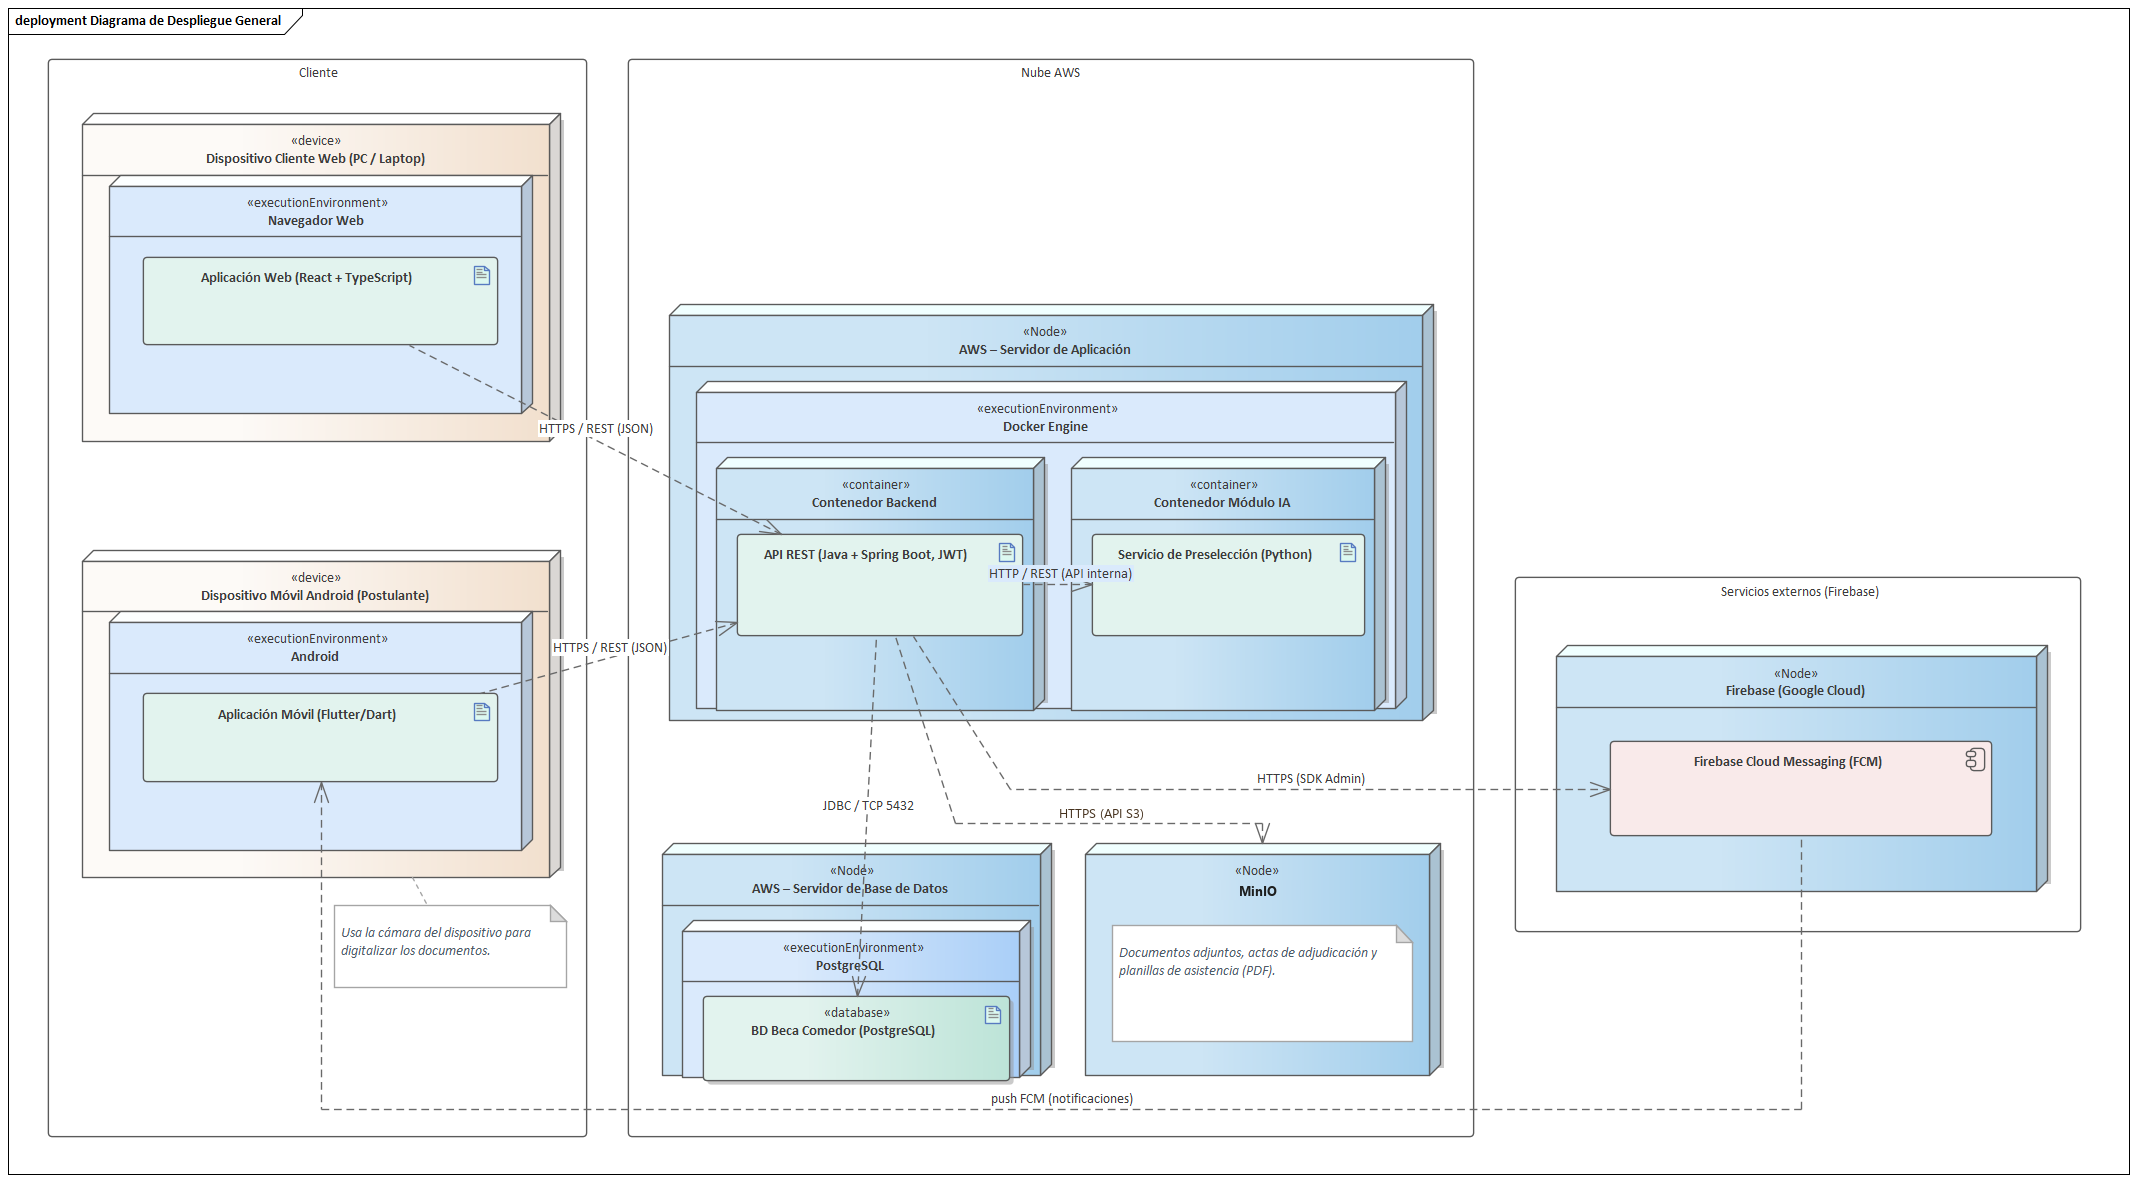
\includegraphics[width=\linewidth,height=0.8\textheight,keepaspectratio]{images/118_Diagrama_Despliegue_General.png}

\smallskip
\noindent\raggedright\textit{Nota.} Elaboración propia.
\end{figure}
\end{landscape}

\subsubsection{7.1.2. Diseño Lógico}\label{sec:cap7_diseno_logico}

El diseño lógico describe la organización interna del sistema en capas y paquetes, independientemente de los nodos físicos en los que se ejecuta (sección~\ref{sec:cap7_diseno_fisico}). Se representa mediante diagramas de paquetes del Lenguaje Unificado de Modelado, en los que cada capa agrupa los paquetes con responsabilidades afines y las dependencias de uso (\textit{use}) se dirigen de las capas superiores hacia las inferiores \parencite{booch2005uml, rumbaugh2004uml}. Este criterio es coherente con el encapsulamiento de los casos de uso en paquetes realizado en el análisis (sección~\ref{sec:cap6_encapsulamiento_cu}), de modo que los seis paquetes funcionales identificados se conservan como módulos de la capa de negocio \parencite{jacobson1999unified}.

\paragraph{Arquitectura lógica general.} La Figura~\ref{fig:diseno_logico_general} presenta la arquitectura lógica general del sistema, organizada en cuatro capas y un paquete de aspectos transversales. La capa de presentación contiene la aplicación web (React y TypeScript) y la aplicación móvil (Flutter), con las que interactúan los usuarios del sistema. La capa de servicios expone la API REST de Spring Boot, con sus controladores y objetos de transferencia de datos, y el mecanismo de autenticación y autorización, que emite y verifica los tokens JWT y aplica el rol del usuario. La capa de negocio agrupa los módulos de cuentas y acceso, convocatoria y postulación, auditoría y adjudicación, becados y asistencia, reportes y trazabilidad, y preselección con inteligencia artificial; este último se implementa en Python como servicio independiente que se consume mediante una API interna. La capa de acceso a datos reúne los repositorios (JPA e Hibernate) y los agentes de servicios externos, que a su vez dependen de la base de datos PostgreSQL y de los servicios externos (notificaciones push, almacenamiento de archivos y módulo de inteligencia artificial). Finalmente, los aspectos transversales (seguridad, bitácora y auditoría de acciones, manejo de errores y validaciones, y notificaciones) son utilizados por todas las capas.

\begin{landscape}
\begin{figure}[p]
\caption{Arquitectura lógica general del sistema en capas}
\label{fig:diseno_logico_general}
\centering
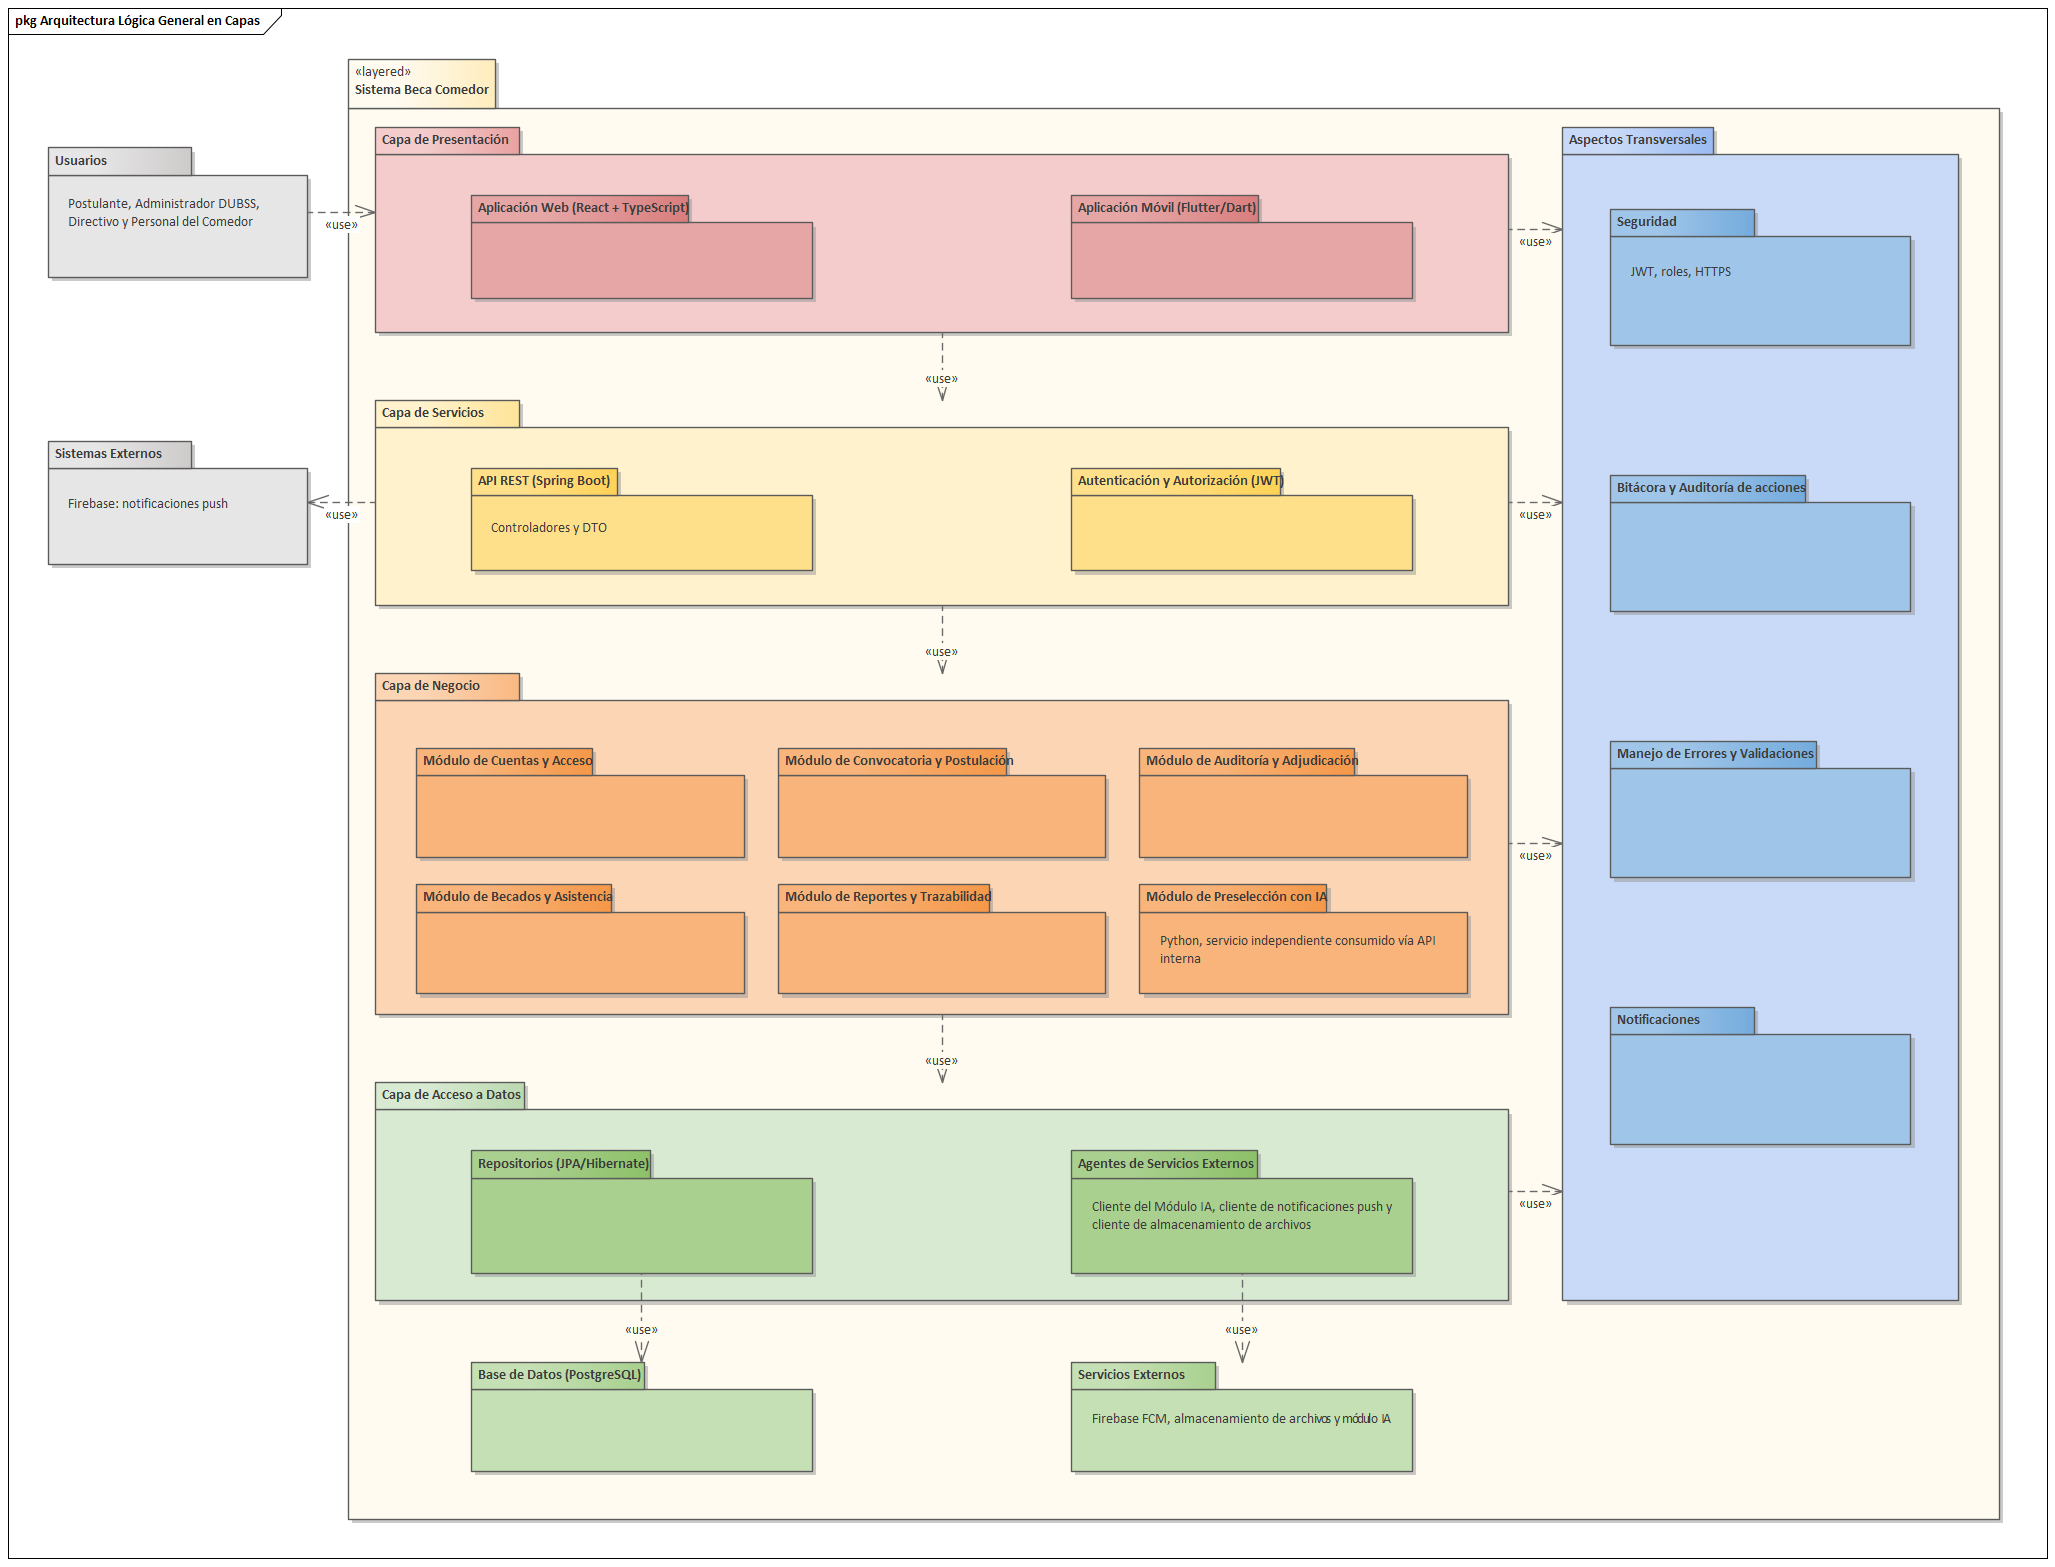
\includegraphics[width=\linewidth,height=0.8\textheight,keepaspectratio]{images/119_Diseno_Logico_Arquitectura_General.png}

\smallskip
\noindent\raggedright\textit{Nota.} Elaboración propia.
\end{figure}
\end{landscape}

\paragraph{Arquitectura lógica del \textit{backend}.} La Figura~\ref{fig:diseno_logico_backend} detalla la organización del \textit{backend} desarrollado con Spring Boot. La capa de presentación (API) contiene los controladores REST y los objetos de transferencia de datos con sus mapeadores; los controladores invocan a los servicios de la capa de lógica de aplicación, que se organizan según los seis paquetes funcionales: cuentas y acceso (P1), convocatoria y postulación (P2), preselección con IA (P3), auditoría y adjudicación (P4), becados y asistencia (P5), y reportes y trazabilidad (P6). Entre estos paquetes existen dependencias que reflejan el flujo del proceso: los servicios de becados y asistencia utilizan los de auditoría y adjudicación, estos utilizan los de convocatoria y postulación, y estos últimos los de preselección con IA. Los servicios operan sobre la capa de dominio, que contiene las entidades y las enumeraciones (por ejemplo, el estado de la postulación), y acceden a la capa de persistencia, conformada por los repositorios JPA, el cliente del módulo de inteligencia artificial y los clientes de notificaciones push y de almacenamiento de archivos. Los repositorios acceden a la base de datos PostgreSQL, y el paquete de seguridad y bitácora es utilizado por todas las capas.

\begin{landscape}
\begin{figure}[p]
\caption{Arquitectura lógica del \textit{backend} (Spring Boot)}
\label{fig:diseno_logico_backend}
\centering
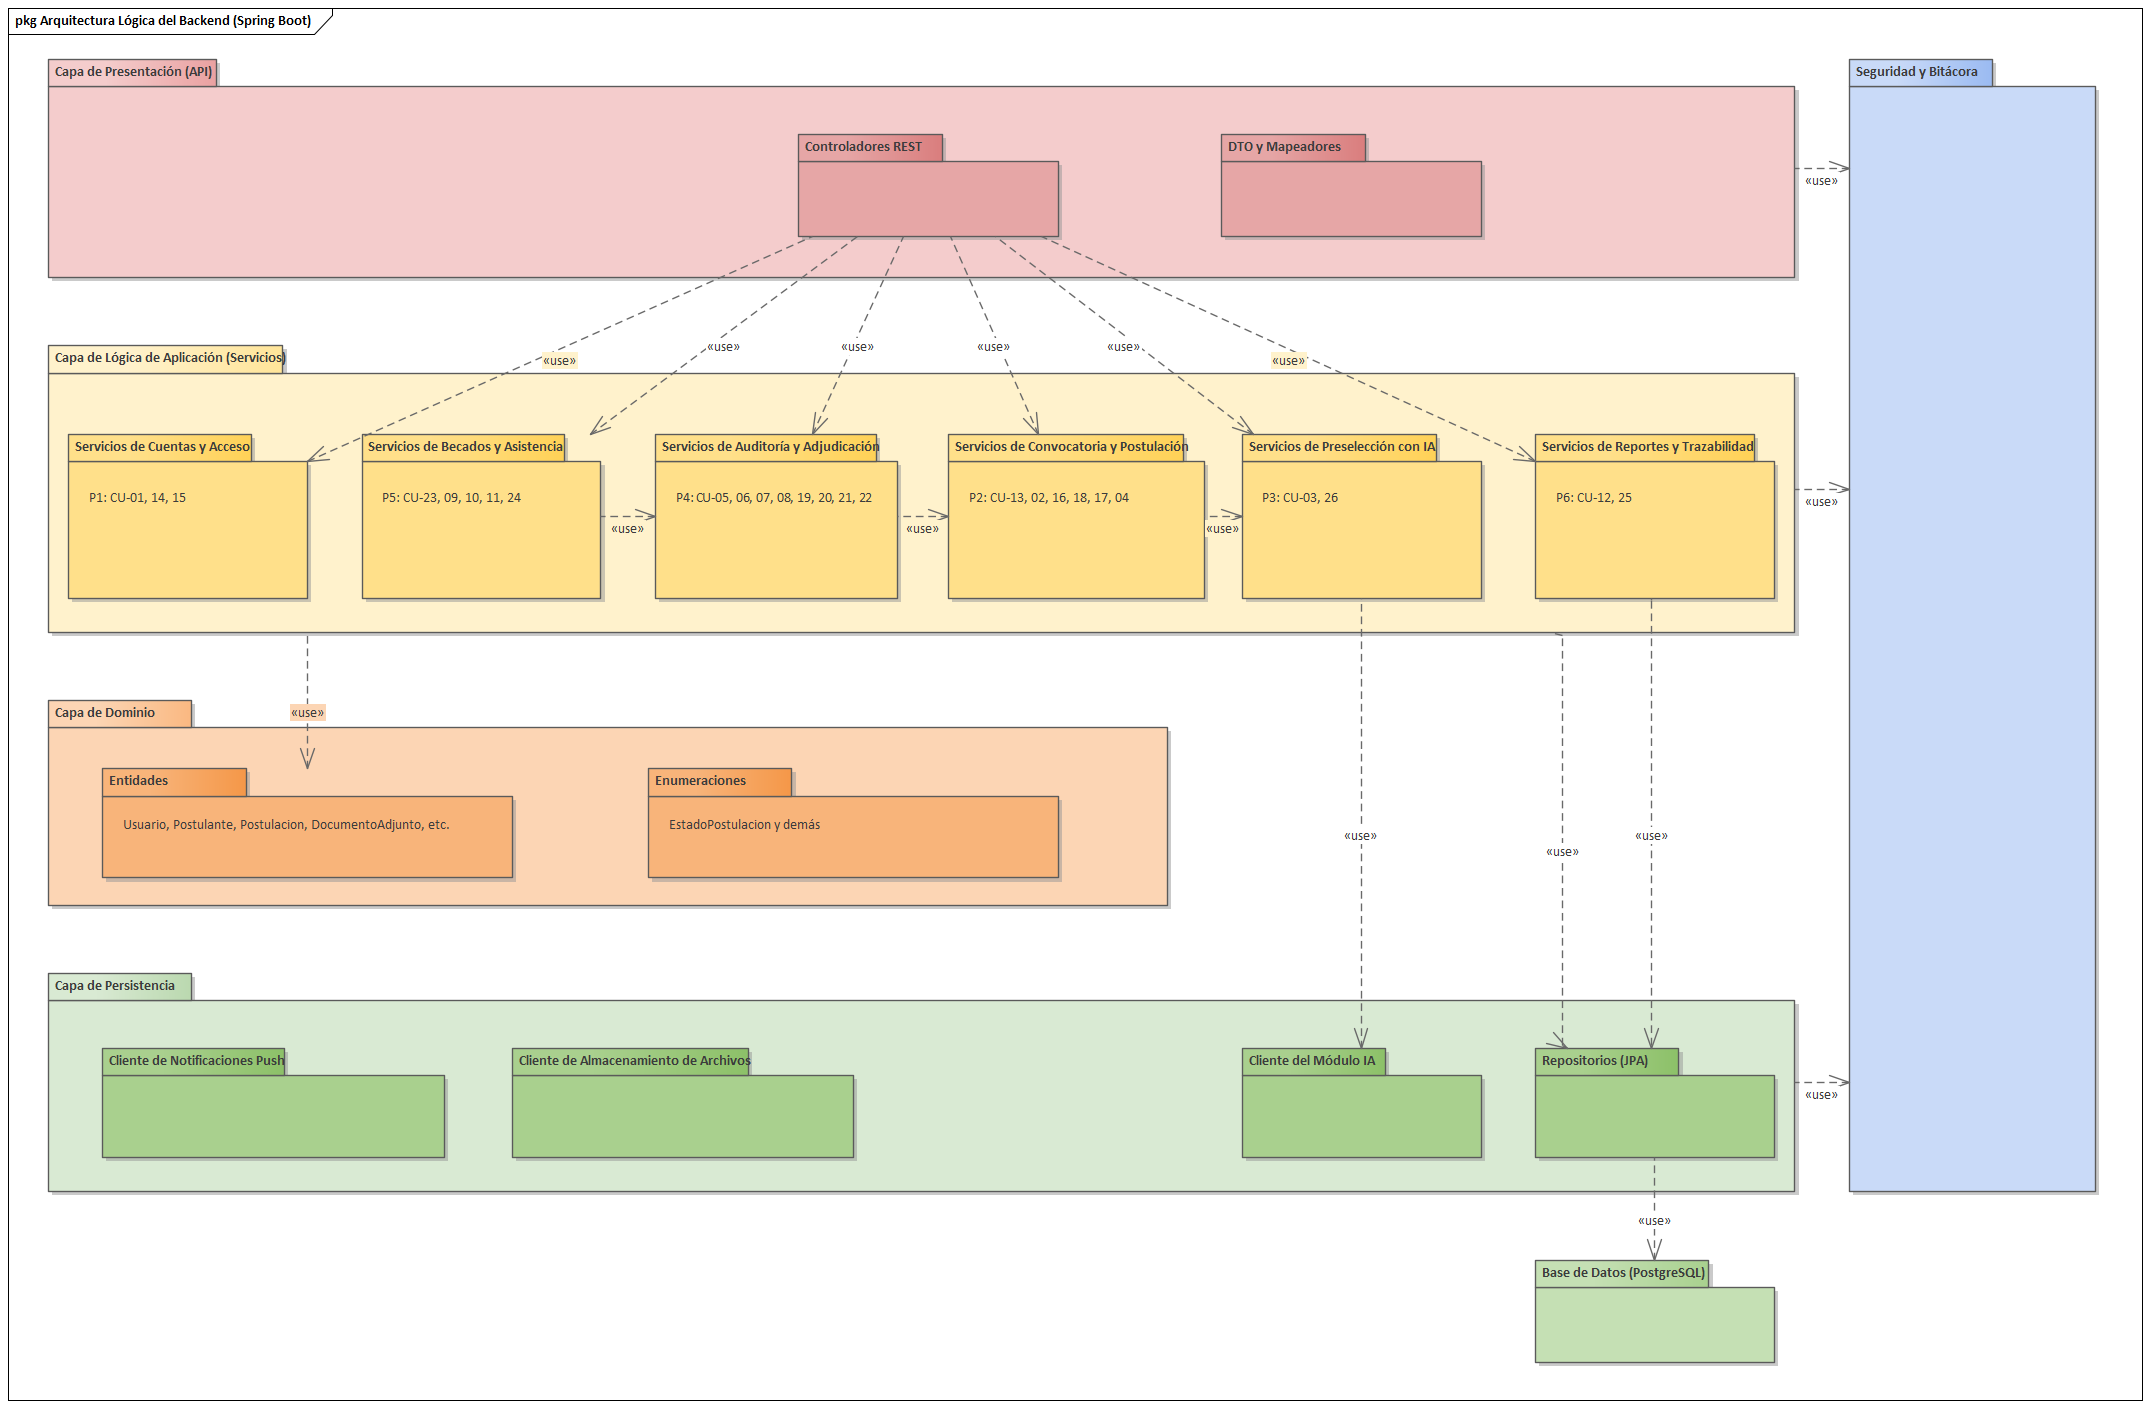
\includegraphics[width=\linewidth,height=0.8\textheight,keepaspectratio]{images/120_Diseno_Logico_Backend.png}

\smallskip
\noindent\raggedright\textit{Nota.} Elaboración propia. P1 a P6 corresponden a los paquetes de casos de uso definidos en el análisis.
\end{figure}
\end{landscape}

% ------------------------------------------------------------------------------
% 7.2. DIAGRAMA DE CLASE
% ------------------------------------------------------------------------------
\wfa{\wn{7}.2. Diagrama de Clase}\label{sec:cap7_diagrama_clase}

El diagrama de clases de diseño integra las clases de entidad identificadas en el análisis de los casos de uso (Capítulo 6) y las refina con sus atributos, tipos de datos, operaciones y relaciones de asociación, composición y herencia, expresadas en el Lenguaje Unificado de Modelado \parencite{booch2005uml}. Las clases representan la información persistente del dominio de la Beca Comedor y se corresponden con las tablas del diseño de datos (sección~\ref{sec:cap7_diseno_datos}); los valores admitidos para los estados y tipos se modelan como enumeraciones.

Todas las clases, excepto \textit{Postulante}, que hereda de \textit{Usuario}, heredan de la clase abstracta \textit{EntidadBase}, que aporta el identificador interno, el código público (UUID) y las fechas de creación, actualización y eliminación lógica; las líneas de esa herencia se omiten en el diagrama para no saturarlo. La Figura~\ref{fig:diagrama_clases} presenta el diagrama de clases del sistema.

\begin{landscape}
\begin{figure}[p]
\caption{Diagrama de clases del sistema}
\label{fig:diagrama_clases}
\centering
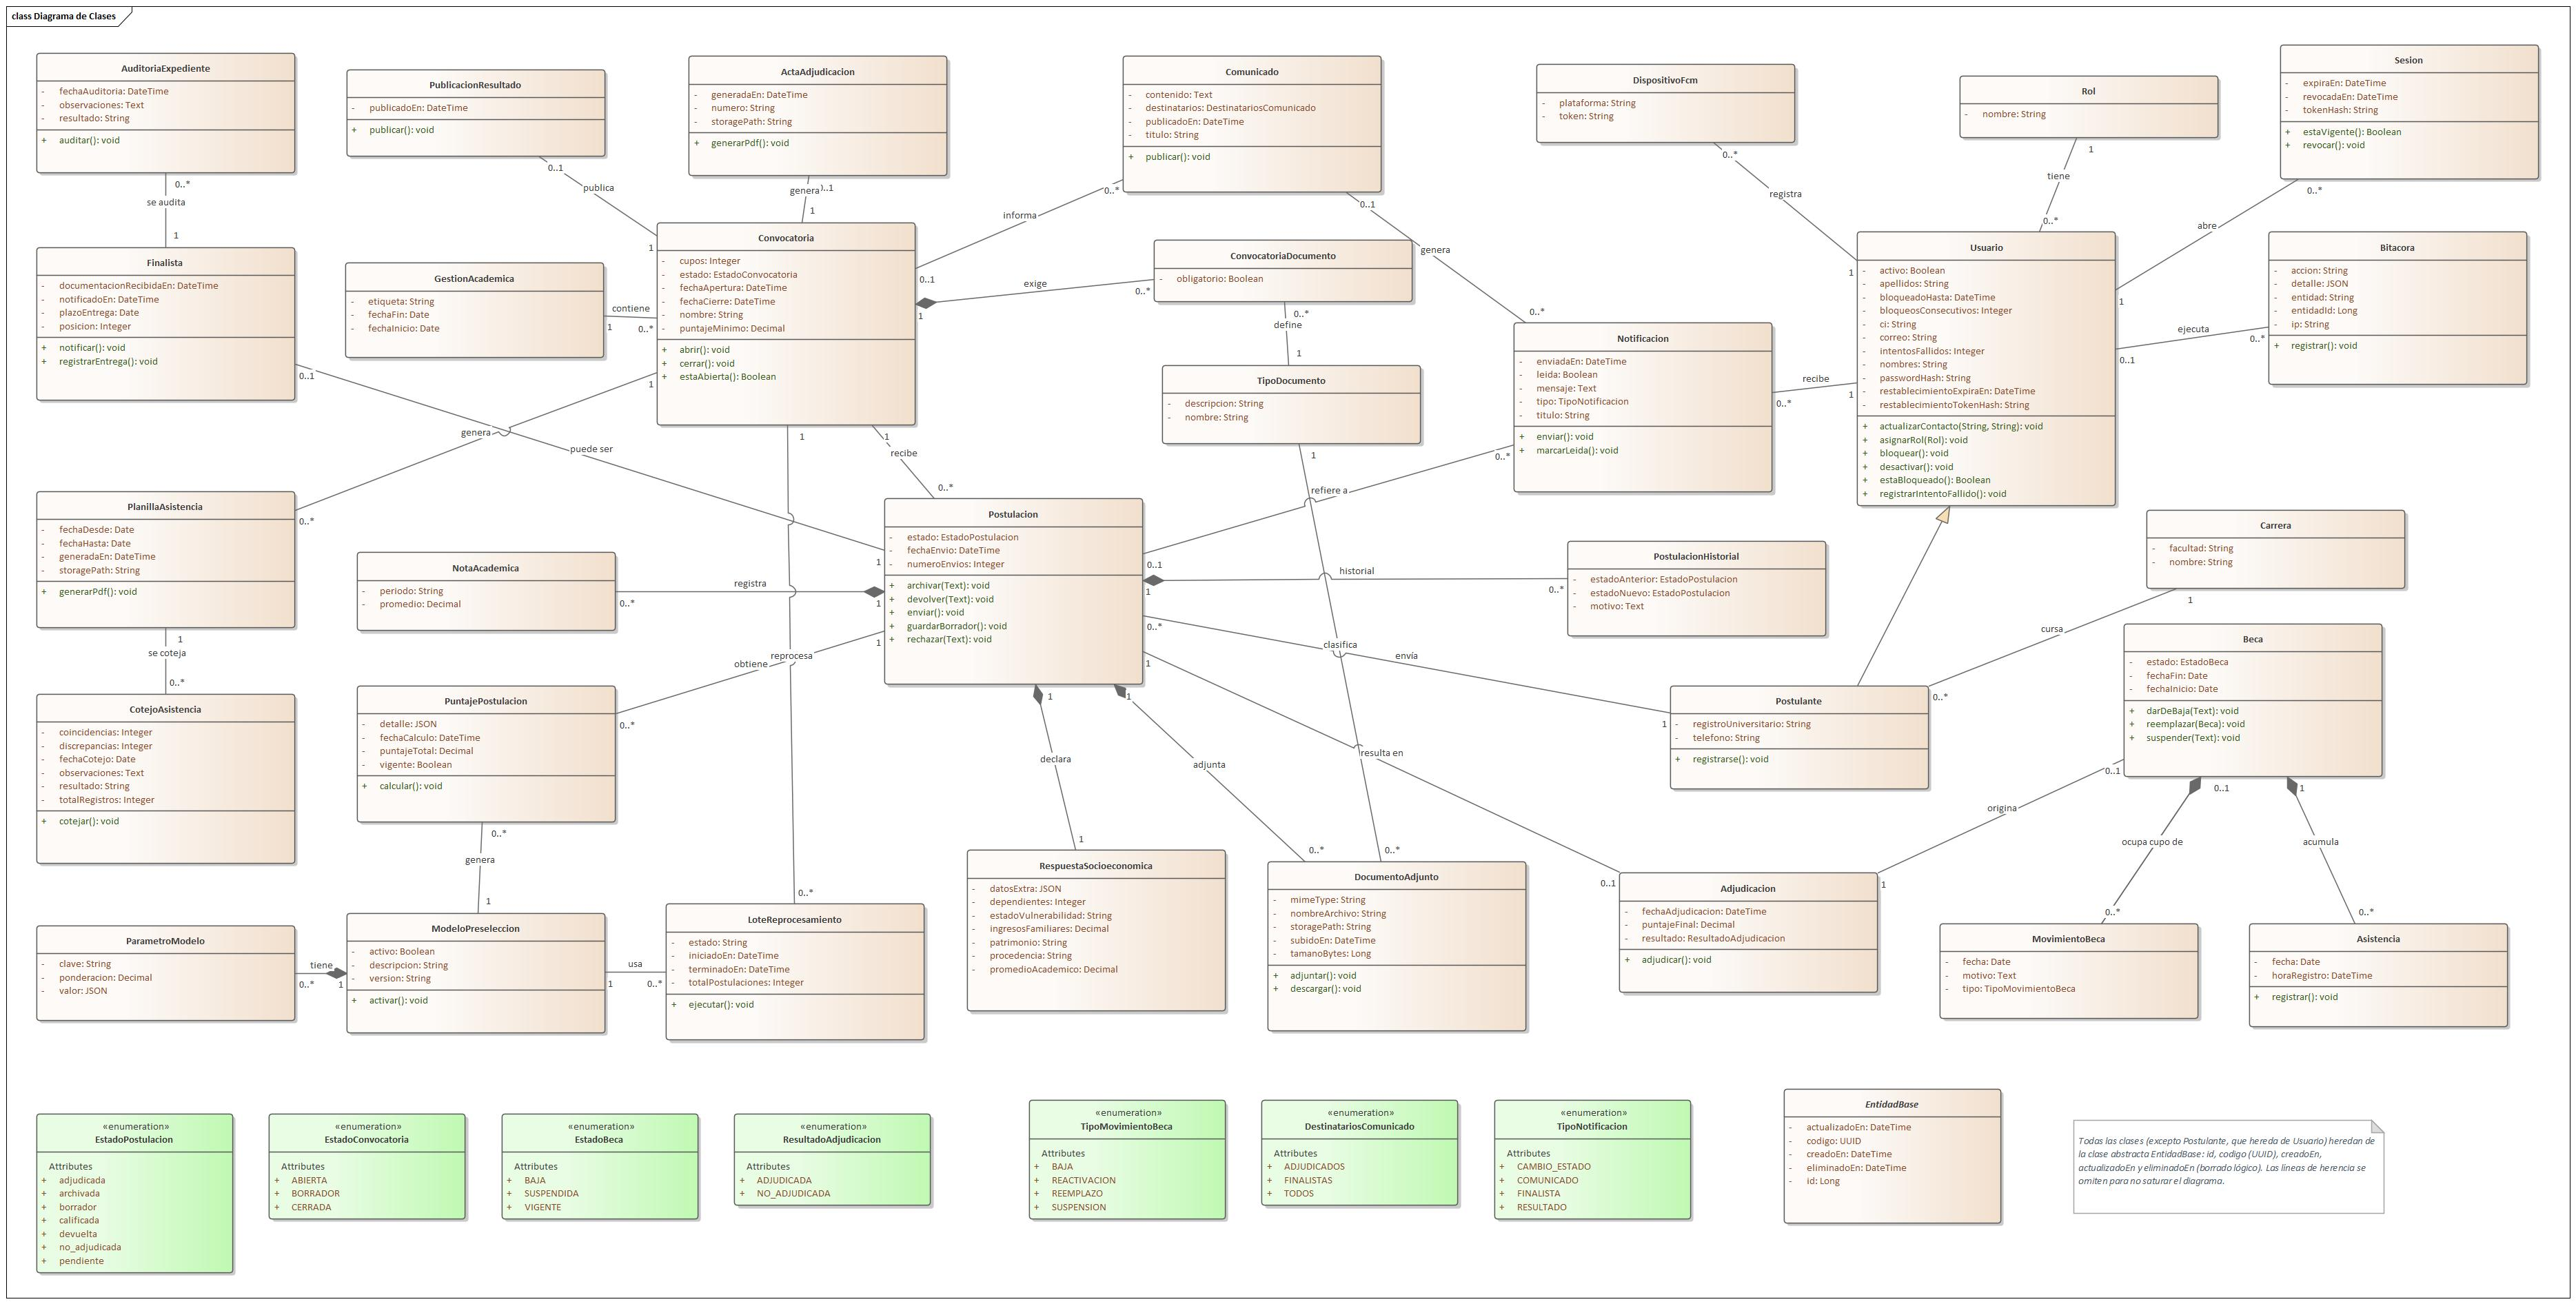
\includegraphics[width=\linewidth,height=0.8\textheight,keepaspectratio]{images/090_Diagrama_de_Clases.jpg}

\smallskip
\noindent\raggedright\textit{Nota.} Elaboración propia.
\end{figure}
\end{landscape}

% ------------------------------------------------------------------------------
% 7.3. DISEÑO DE DATOS
% ------------------------------------------------------------------------------
\wfa{\wn{7}.3. Diseño de Datos}\label{sec:cap7_diseno_datos}

El diseño de datos traduce las clases persistentes del diagrama de clases (sección~\ref{sec:cap7_diagrama_clase}) a un modelo relacional implementado en PostgreSQL. El modelo consta de 31 tablas agrupadas según los seis paquetes del análisis: Cuentas y acceso (4), Convocatoria y postulación (9), Preselección con IA (4), Auditoría y adjudicación (8), Becados y asistencia (5) y Reportes y trazabilidad (1). Los nombres de tablas y columnas se escriben en minúsculas, en singular y separados por guion bajo; cada tabla tiene una clave primaria interna \textit{id} y las claves foráneas se nombran \textit{\textless{}tabla\textgreater{}\_id}.

Todas las tablas incorporan cuatro columnas comunes: \textit{codigo\_\textless{}tabla\textgreater{}}, un identificador público UUID versión 7, único y no nulo, que es el único identificador que se expone a la API y a los clientes web y móvil; \textit{creado\_en} y \textit{actualizado\_en}, que registran la fecha y hora de creación y de la última modificación; y \textit{eliminado\_en}, que implementa el borrado lógico, de modo que ningún registro se elimina físicamente. Las contraseñas no se almacenan en la base de datos, pues las gestiona Firebase Authentication, y los archivos se guardan en Firebase Storage, del que la base de datos solo conserva la ruta.

\wfb{\wn{7}.3.1. Diseño de Datos Lógico}\label{sec:cap7_datos_logico}

\wfc{\wn{7}.3.1.1. Diseño lógico de la Base de Datos.}\label{sec:cap7_logico_bd}
El diseño lógico de la base de datos representa cada tabla con sus columnas, tipos de datos, claves primarias (PK), claves foráneas (FK) y restricciones de unicidad (UQ), así como las relaciones y cardinalidades entre las tablas. La Figura~\ref{fig:diseno_logico_bd} presenta el diagrama del diseño lógico.

\begin{figure}[H]
\caption{Diseño lógico de la base de datos}
\label{fig:diseno_logico_bd}
\centering
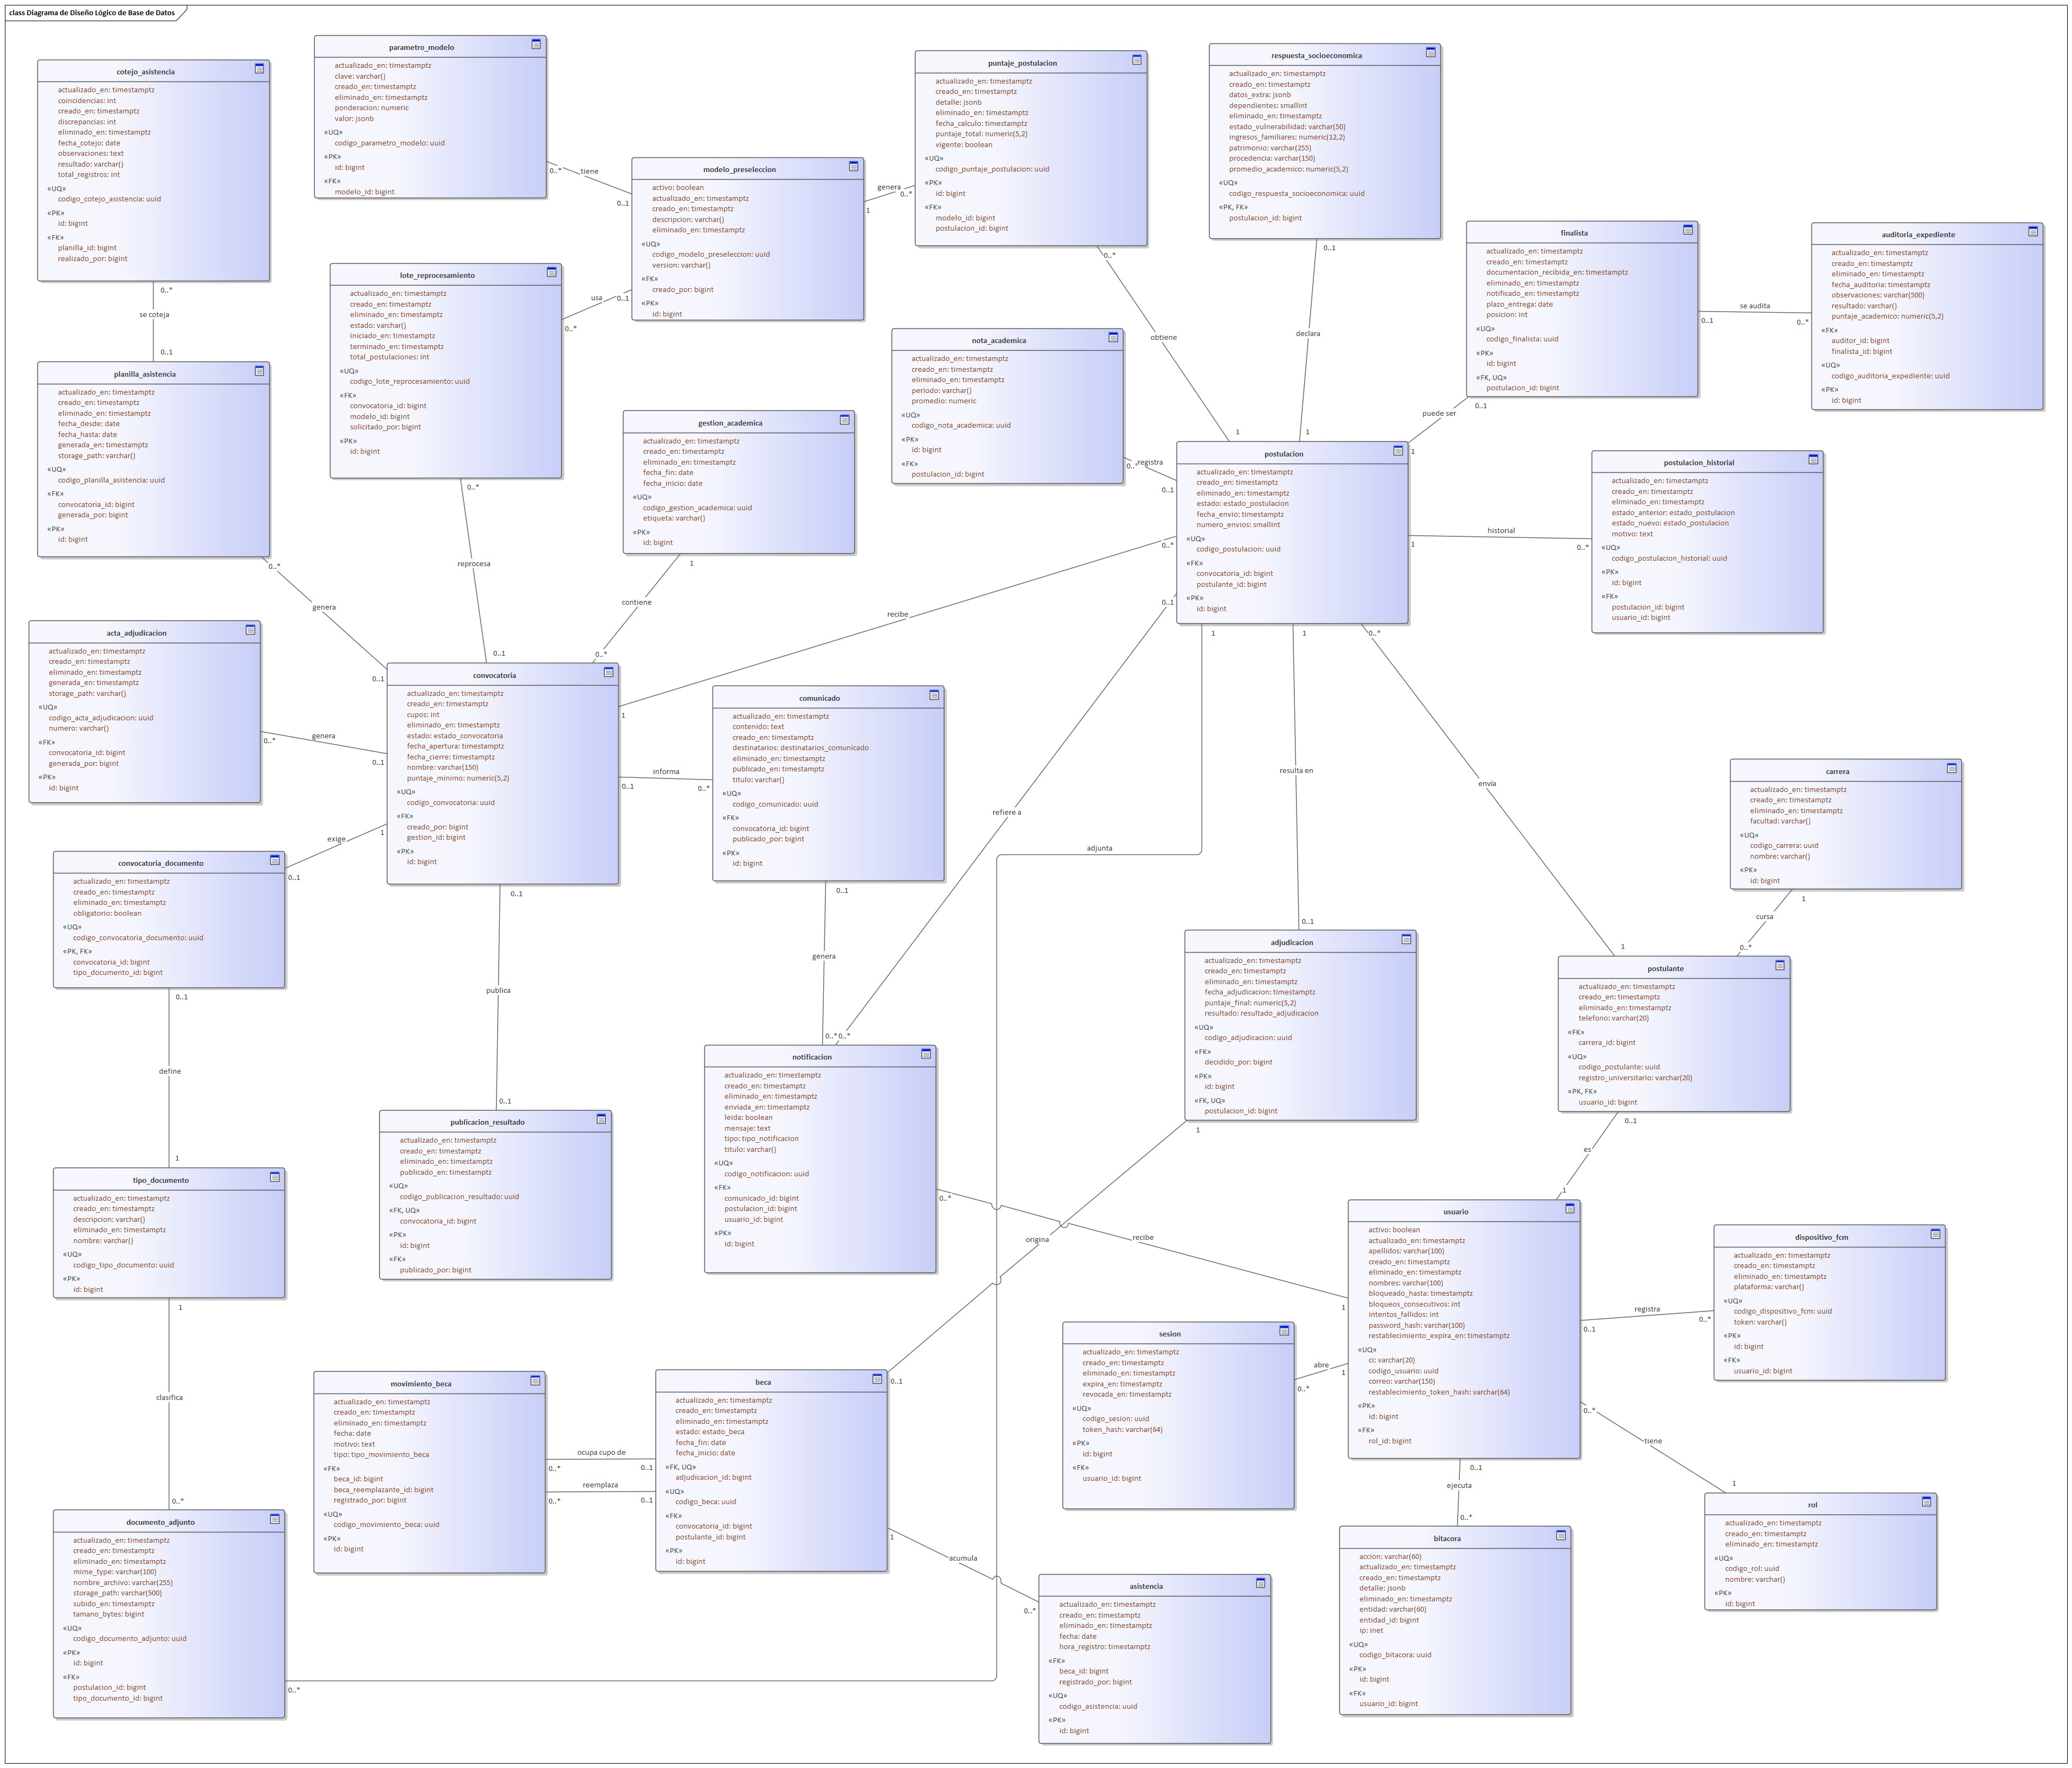
\includegraphics[width=\textwidth,height=0.8\textheight,keepaspectratio]{images/091_Diseno_Logico_Base_de_Datos.jpg}

\smallskip
\noindent\raggedright\textit{Nota.} Elaboración propia.
\end{figure}

\wfc{\wn{7}.3.1.2. Mapeo.}\label{sec:cap7_mapeo}
El mapeo presenta, para cada una de las 31 tablas del diseño lógico, sus atributos y el tipo de dato asignado a cada uno, indicando entre paréntesis las claves primarias (PK), foráneas (FK) y únicas (UQ). Las tablas se presentan agrupadas por paquete, en el mismo orden del diseño lógico.

% ------------------------------------------------------------------------------
% 7.3.1.2. MAPEO (generado a partir del diagrama lógico de la base de datos)
% ------------------------------------------------------------------------------

\begin{table}[H]
\caption{Mapeo de la tabla rol}
\label{tab:mapeo_rol}
\centering
\footnotesize\linespread{1}\selectfont
\renewcommand{\arraystretch}{1.3}
\begin{tabular}{*{5}{>{\centering\arraybackslash}p{2.85cm}}}
\toprule
\textbf{id (PK)} & \textbf{nombre (UQ)} & \textbf{codigo\_\allowbreak{}rol (UQ)} & \textbf{creado\_\allowbreak{}en} & \textbf{actualizado\_\allowbreak{}en} \\
\midrule
bigint & varchar(50) & uuid & timestamptz & timestamptz \\
\bottomrule
\end{tabular}

\vspace{14pt}
\begin{tabular}{*{5}{>{\centering\arraybackslash}p{2.85cm}}}
\toprule
\textbf{eliminado\_\allowbreak{}en} &  &  &  &  \\
\midrule
timestamptz &  &  &  &  \\
\bottomrule
\end{tabular}

\smallskip
\noindent\raggedright\textit{Nota.} Elaboración propia.
\end{table}

\begin{table}[H]
\caption{Mapeo de la tabla usuario}
\label{tab:mapeo_usuario}
\centering
\footnotesize\linespread{1}\selectfont
\renewcommand{\arraystretch}{1.3}
\begin{tabular}{*{5}{>{\centering\arraybackslash}p{2.85cm}}}
\toprule
\textbf{id (PK)} & \textbf{ci (UQ)} & \textbf{correo (UQ)} & \textbf{nombres} & \textbf{apellidos} \\
\midrule
bigint & varchar(20) & varchar(150) & varchar(100) & varchar(100) \\
\bottomrule
\end{tabular}

\vspace{14pt}
\begin{tabular}{*{5}{>{\centering\arraybackslash}p{2.85cm}}}
\toprule
\textbf{password\_\allowbreak{}hash} & \textbf{activo} & \textbf{rol\_\allowbreak{}id (FK)} & \textbf{codigo\_\allowbreak{}usuario (UQ)} & \textbf{intentos\_\allowbreak{}fallidos} \\
\midrule
varchar(100) & boolean & bigint & uuid & integer \\
\bottomrule
\end{tabular}

\vspace{14pt}
\begin{tabular}{*{5}{>{\centering\arraybackslash}p{2.85cm}}}
\toprule
\textbf{bloqueos\_\allowbreak{}consecutivos} & \textbf{bloqueado\_\allowbreak{}hasta} & \textbf{creado\_\allowbreak{}en} & \textbf{actualizado\_\allowbreak{}en} & \textbf{eliminado\_\allowbreak{}en} \\
\midrule
integer & timestamptz & timestamptz & timestamptz & timestamptz \\
\bottomrule
\end{tabular}

\smallskip
\noindent\raggedright\textit{Nota.} Elaboración propia.
\end{table}

\begin{table}[H]
\caption{Mapeo de la tabla carrera}
\label{tab:mapeo_carrera}
\centering
\footnotesize\linespread{1}\selectfont
\renewcommand{\arraystretch}{1.3}
\begin{tabular}{*{5}{>{\centering\arraybackslash}p{2.85cm}}}
\toprule
\textbf{id (PK)} & \textbf{nombre (UQ)} & \textbf{facultad} & \textbf{codigo\_\allowbreak{}carrera (UQ)} & \textbf{creado\_\allowbreak{}en} \\
\midrule
bigint & varchar(150) & varchar(150) & uuid & timestamptz \\
\bottomrule
\end{tabular}

\vspace{14pt}
\begin{tabular}{*{5}{>{\centering\arraybackslash}p{2.85cm}}}
\toprule
\textbf{actualizado\_\allowbreak{}en} & \textbf{eliminado\_\allowbreak{}en} &  &  &  \\
\midrule
timestamptz & timestamptz &  &  &  \\
\bottomrule
\end{tabular}

\smallskip
\noindent\raggedright\textit{Nota.} Elaboración propia.
\end{table}

\begin{table}[H]
\caption{Mapeo de la tabla sesion}
\label{tab:mapeo_sesion}
\centering
\footnotesize\linespread{1}\selectfont
\renewcommand{\arraystretch}{1.3}
\begin{tabular}{*{5}{>{\centering\arraybackslash}p{2.85cm}}}
\toprule
\textbf{id (PK)} & \textbf{usuario\_\allowbreak{}id (FK)} & \textbf{codigo\_\allowbreak{}sesion (UQ)} & \textbf{token\_\allowbreak{}hash (UQ)} & \textbf{expira\_\allowbreak{}en} \\
\midrule
bigint & bigint & uuid & varchar(64) & timestamptz \\
\bottomrule
\end{tabular}

\vspace{14pt}
\begin{tabular}{*{5}{>{\centering\arraybackslash}p{2.85cm}}}
\toprule
\textbf{revocada\_\allowbreak{}en} & \textbf{creado\_\allowbreak{}en} & \textbf{actualizado\_\allowbreak{}en} & \textbf{eliminado\_\allowbreak{}en} &  \\
\midrule
timestamptz & timestamptz & timestamptz & timestamptz &  \\
\bottomrule
\end{tabular}

\smallskip
\noindent\raggedright\textit{Nota.} Elaboración propia.
\end{table}

\begin{table}[H]
\caption{Mapeo de la tabla postulante}
\label{tab:mapeo_postulante}
\centering
\footnotesize\linespread{1}\selectfont
\renewcommand{\arraystretch}{1.3}
\begin{tabular}{*{5}{>{\centering\arraybackslash}p{2.85cm}}}
\toprule
\textbf{usuario\_\allowbreak{}id (PK, FK)} & \textbf{carrera\_\allowbreak{}id (FK)} & \textbf{registro\_\allowbreak{}universitario (UQ)} & \textbf{telefono} & \textbf{codigo\_\allowbreak{}postulante (UQ)} \\
\midrule
bigint & bigint & varchar(20) & varchar(20) & uuid \\
\bottomrule
\end{tabular}

\vspace{14pt}
\begin{tabular}{*{5}{>{\centering\arraybackslash}p{2.85cm}}}
\toprule
\textbf{creado\_\allowbreak{}en} & \textbf{actualizado\_\allowbreak{}en} & \textbf{eliminado\_\allowbreak{}en} &  &  \\
\midrule
timestamptz & timestamptz & timestamptz &  &  \\
\bottomrule
\end{tabular}

\smallskip
\noindent\raggedright\textit{Nota.} Elaboración propia.
\end{table}

\begin{table}[H]
\caption{Mapeo de la tabla gestion\_\allowbreak{}academica}
\label{tab:mapeo_gestion_academica}
\centering
\footnotesize\linespread{1}\selectfont
\renewcommand{\arraystretch}{1.3}
\begin{tabular}{*{5}{>{\centering\arraybackslash}p{2.85cm}}}
\toprule
\textbf{id (PK)} & \textbf{etiqueta (UQ)} & \textbf{fecha\_\allowbreak{}inicio} & \textbf{fecha\_\allowbreak{}fin} & \textbf{codigo\_\allowbreak{}gestion\_\allowbreak{}academica (UQ)} \\
\midrule
bigint & varchar(20) & date & date & uuid \\
\bottomrule
\end{tabular}

\vspace{14pt}
\begin{tabular}{*{5}{>{\centering\arraybackslash}p{2.85cm}}}
\toprule
\textbf{creado\_\allowbreak{}en} & \textbf{actualizado\_\allowbreak{}en} & \textbf{eliminado\_\allowbreak{}en} &  &  \\
\midrule
timestamptz & timestamptz & timestamptz &  &  \\
\bottomrule
\end{tabular}

\smallskip
\noindent\raggedright\textit{Nota.} Elaboración propia.
\end{table}

\begin{table}[H]
\caption{Mapeo de la tabla convocatoria}
\label{tab:mapeo_convocatoria}
\centering
\footnotesize\linespread{1}\selectfont
\renewcommand{\arraystretch}{1.3}
\begin{tabular}{*{5}{>{\centering\arraybackslash}p{2.85cm}}}
\toprule
\textbf{id (PK)} & \textbf{gestion\_\allowbreak{}id (FK)} & \textbf{nombre} & \textbf{fecha\_\allowbreak{}apertura} & \textbf{fecha\_\allowbreak{}cierre} \\
\midrule
bigint & bigint & varchar(150) & timestamptz & timestamptz \\
\bottomrule
\end{tabular}

\vspace{14pt}
\begin{tabular}{*{5}{>{\centering\arraybackslash}p{2.85cm}}}
\toprule
\textbf{cupos} & \textbf{puntaje\_\allowbreak{}minimo} & \textbf{estado} & \textbf{creado\_\allowbreak{}por (FK)} & \textbf{codigo\_\allowbreak{}convocatoria (UQ)} \\
\midrule
integer & numeric(5,2) & estado\_\allowbreak{}convocatoria & bigint & uuid \\
\bottomrule
\end{tabular}

\vspace{14pt}
\begin{tabular}{*{5}{>{\centering\arraybackslash}p{2.85cm}}}
\toprule
\textbf{creado\_\allowbreak{}en} & \textbf{actualizado\_\allowbreak{}en} & \textbf{eliminado\_\allowbreak{}en} &  &  \\
\midrule
timestamptz & timestamptz & timestamptz &  &  \\
\bottomrule
\end{tabular}

\smallskip
\noindent\raggedright\textit{Nota.} Elaboración propia.
\end{table}

\begin{table}[H]
\caption{Mapeo de la tabla tipo\_\allowbreak{}documento}
\label{tab:mapeo_tipo_documento}
\centering
\footnotesize\linespread{1}\selectfont
\renewcommand{\arraystretch}{1.3}
\begin{tabular}{*{5}{>{\centering\arraybackslash}p{2.85cm}}}
\toprule
\textbf{id (PK)} & \textbf{nombre} & \textbf{descripcion} & \textbf{codigo\_\allowbreak{}tipo\_\allowbreak{}documento (UQ)} & \textbf{creado\_\allowbreak{}en} \\
\midrule
bigint & varchar(100) & varchar(255) & uuid & timestamptz \\
\bottomrule
\end{tabular}

\vspace{14pt}
\begin{tabular}{*{5}{>{\centering\arraybackslash}p{2.85cm}}}
\toprule
\textbf{actualizado\_\allowbreak{}en} & \textbf{eliminado\_\allowbreak{}en} &  &  &  \\
\midrule
timestamptz & timestamptz &  &  &  \\
\bottomrule
\end{tabular}

\smallskip
\noindent\raggedright\textit{Nota.} Elaboración propia.
\end{table}

\begin{table}[H]
\caption{Mapeo de la tabla convocatoria\_\allowbreak{}documento}
\label{tab:mapeo_convocatoria_documento}
\centering
\footnotesize\linespread{1}\selectfont
\renewcommand{\arraystretch}{1.3}
\begin{tabular}{*{5}{>{\centering\arraybackslash}p{2.85cm}}}
\toprule
\textbf{convocatoria\_\allowbreak{}id (PK, FK)} & \textbf{tipo\_\allowbreak{}documento\_\allowbreak{}id (PK, FK)} & \textbf{obligatorio} & \textbf{codigo\_\allowbreak{}convocatoria\_\allowbreak{}documento (UQ)} & \textbf{creado\_\allowbreak{}en} \\
\midrule
bigint & bigint & boolean & uuid & timestamptz \\
\bottomrule
\end{tabular}

\vspace{14pt}
\begin{tabular}{*{5}{>{\centering\arraybackslash}p{2.85cm}}}
\toprule
\textbf{actualizado\_\allowbreak{}en} & \textbf{eliminado\_\allowbreak{}en} &  &  &  \\
\midrule
timestamptz & timestamptz &  &  &  \\
\bottomrule
\end{tabular}

\smallskip
\noindent\raggedright\textit{Nota.} Elaboración propia.
\end{table}

\begin{table}[H]
\caption{Mapeo de la tabla postulacion}
\label{tab:mapeo_postulacion}
\centering
\footnotesize\linespread{1}\selectfont
\renewcommand{\arraystretch}{1.3}
\begin{tabular}{*{5}{>{\centering\arraybackslash}p{2.85cm}}}
\toprule
\textbf{id (PK)} & \textbf{postulante\_\allowbreak{}id (FK)} & \textbf{convocatoria\_\allowbreak{}id (FK)} & \textbf{estado} & \textbf{fecha\_\allowbreak{}envio} \\
\midrule
bigint & bigint & bigint & estado\_\allowbreak{}postulacion & timestamptz \\
\bottomrule
\end{tabular}

\vspace{14pt}
\begin{tabular}{*{5}{>{\centering\arraybackslash}p{2.85cm}}}
\toprule
\textbf{numero\_\allowbreak{}envios} & \textbf{codigo\_\allowbreak{}postulacion (UQ)} & \textbf{creado\_\allowbreak{}en} & \textbf{actualizado\_\allowbreak{}en} & \textbf{eliminado\_\allowbreak{}en} \\
\midrule
smallint & uuid & timestamptz & timestamptz & timestamptz \\
\bottomrule
\end{tabular}

\smallskip
\noindent\raggedright\textit{Nota.} Elaboración propia.
\end{table}

\begin{table}[H]
\caption{Mapeo de la tabla respuesta\_\allowbreak{}socioeconomica}
\label{tab:mapeo_respuesta_socioeconomica}
\centering
\footnotesize\linespread{1}\selectfont
\renewcommand{\arraystretch}{1.3}
\begin{tabular}{*{5}{>{\centering\arraybackslash}p{2.85cm}}}
\toprule
\textbf{postulacion\_\allowbreak{}id (PK, FK)} & \textbf{ingresos\_\allowbreak{}familiares} & \textbf{dependientes} & \textbf{procedencia} & \textbf{patrimonio} \\
\midrule
bigint & numeric(12,2) & smallint & varchar(150) & varchar(255) \\
\bottomrule
\end{tabular}

\vspace{14pt}
\begin{tabular}{*{5}{>{\centering\arraybackslash}p{2.85cm}}}
\toprule
\textbf{estado\_\allowbreak{}vulnerabilidad} & \textbf{promedio\_\allowbreak{}academico} & \textbf{datos\_\allowbreak{}extra} & \textbf{codigo\_\allowbreak{}respuesta\_\allowbreak{}socioeconomica (UQ)} & \textbf{creado\_\allowbreak{}en} \\
\midrule
varchar(50) & numeric(5,2) & jsonb & uuid & timestamptz \\
\bottomrule
\end{tabular}

\vspace{14pt}
\begin{tabular}{*{5}{>{\centering\arraybackslash}p{2.85cm}}}
\toprule
\textbf{actualizado\_\allowbreak{}en} & \textbf{eliminado\_\allowbreak{}en} &  &  &  \\
\midrule
timestamptz & timestamptz &  &  &  \\
\bottomrule
\end{tabular}

\smallskip
\noindent\raggedright\textit{Nota.} Elaboración propia.
\end{table}

\begin{table}[H]
\caption{Mapeo de la tabla nota\_\allowbreak{}academica}
\label{tab:mapeo_nota_academica}
\centering
\footnotesize\linespread{1}\selectfont
\renewcommand{\arraystretch}{1.3}
\begin{tabular}{*{5}{>{\centering\arraybackslash}p{2.85cm}}}
\toprule
\textbf{id (PK)} & \textbf{postulacion\_\allowbreak{}id (FK)} & \textbf{periodo} & \textbf{promedio} & \textbf{codigo\_\allowbreak{}nota\_\allowbreak{}academica (UQ)} \\
\midrule
bigint & bigint & varchar(20) & numeric & uuid \\
\bottomrule
\end{tabular}

\vspace{14pt}
\begin{tabular}{*{5}{>{\centering\arraybackslash}p{2.85cm}}}
\toprule
\textbf{creado\_\allowbreak{}en} & \textbf{actualizado\_\allowbreak{}en} & \textbf{eliminado\_\allowbreak{}en} &  &  \\
\midrule
timestamptz & timestamptz & timestamptz &  &  \\
\bottomrule
\end{tabular}

\smallskip
\noindent\raggedright\textit{Nota.} Elaboración propia.
\end{table}

\begin{table}[H]
\caption{Mapeo de la tabla documento\_\allowbreak{}adjunto}
\label{tab:mapeo_documento_adjunto}
\centering
\footnotesize\linespread{1}\selectfont
\renewcommand{\arraystretch}{1.3}
\begin{tabular}{*{5}{>{\centering\arraybackslash}p{2.85cm}}}
\toprule
\textbf{id (PK)} & \textbf{postulacion\_\allowbreak{}id (FK)} & \textbf{tipo\_\allowbreak{}documento\_\allowbreak{}id (FK)} & \textbf{nombre\_\allowbreak{}archivo} & \textbf{storage\_\allowbreak{}path} \\
\midrule
bigint & bigint & bigint & varchar(255) & varchar(500) \\
\bottomrule
\end{tabular}

\vspace{14pt}
\begin{tabular}{*{5}{>{\centering\arraybackslash}p{2.85cm}}}
\toprule
\textbf{mime\_\allowbreak{}type} & \textbf{tamano\_\allowbreak{}bytes} & \textbf{subido\_\allowbreak{}en} & \textbf{codigo\_\allowbreak{}documento\_\allowbreak{}adjunto (UQ)} & \textbf{creado\_\allowbreak{}en} \\
\midrule
varchar(100) & bigint & timestamptz & uuid & timestamptz \\
\bottomrule
\end{tabular}

\vspace{14pt}
\begin{tabular}{*{5}{>{\centering\arraybackslash}p{2.85cm}}}
\toprule
\textbf{actualizado\_\allowbreak{}en} & \textbf{eliminado\_\allowbreak{}en} &  &  &  \\
\midrule
timestamptz & timestamptz &  &  &  \\
\bottomrule
\end{tabular}

\smallskip
\noindent\raggedright\textit{Nota.} Elaboración propia.
\end{table}

\begin{table}[H]
\caption{Mapeo de la tabla postulacion\_\allowbreak{}historial}
\label{tab:mapeo_postulacion_historial}
\centering
\footnotesize\linespread{1}\selectfont
\renewcommand{\arraystretch}{1.3}
\begin{tabular}{*{5}{>{\centering\arraybackslash}p{2.85cm}}}
\toprule
\textbf{id (PK)} & \textbf{postulacion\_\allowbreak{}id (FK)} & \textbf{estado\_\allowbreak{}anterior} & \textbf{estado\_\allowbreak{}nuevo} & \textbf{usuario\_\allowbreak{}id (FK)} \\
\midrule
bigint & bigint & estado\_\allowbreak{}postulacion & estado\_\allowbreak{}postulacion & bigint \\
\bottomrule
\end{tabular}

\vspace{14pt}
\begin{tabular}{*{5}{>{\centering\arraybackslash}p{2.85cm}}}
\toprule
\textbf{motivo} & \textbf{codigo\_\allowbreak{}postulacion\_\allowbreak{}historial (UQ)} & \textbf{creado\_\allowbreak{}en} & \textbf{actualizado\_\allowbreak{}en} & \textbf{eliminado\_\allowbreak{}en} \\
\midrule
text & uuid & timestamptz & timestamptz & timestamptz \\
\bottomrule
\end{tabular}

\smallskip
\noindent\raggedright\textit{Nota.} Elaboración propia.
\end{table}

\begin{table}[H]
\caption{Mapeo de la tabla modelo\_\allowbreak{}preseleccion}
\label{tab:mapeo_modelo_preseleccion}
\centering
\footnotesize\linespread{1}\selectfont
\renewcommand{\arraystretch}{1.3}
\begin{tabular}{*{5}{>{\centering\arraybackslash}p{2.85cm}}}
\toprule
\textbf{id (PK)} & \textbf{version (UQ)} & \textbf{descripcion} & \textbf{activo} & \textbf{creado\_\allowbreak{}por (FK)} \\
\midrule
bigint & varchar(20) & varchar(255) & boolean & bigint \\
\bottomrule
\end{tabular}

\vspace{14pt}
\begin{tabular}{*{5}{>{\centering\arraybackslash}p{2.85cm}}}
\toprule
\textbf{codigo\_\allowbreak{}modelo\_\allowbreak{}preseleccion (UQ)} & \textbf{creado\_\allowbreak{}en} & \textbf{actualizado\_\allowbreak{}en} & \textbf{eliminado\_\allowbreak{}en} &  \\
\midrule
uuid & timestamptz & timestamptz & timestamptz &  \\
\bottomrule
\end{tabular}

\smallskip
\noindent\raggedright\textit{Nota.} Elaboración propia.
\end{table}

\begin{table}[H]
\caption{Mapeo de la tabla parametro\_\allowbreak{}modelo}
\label{tab:mapeo_parametro_modelo}
\centering
\footnotesize\linespread{1}\selectfont
\renewcommand{\arraystretch}{1.3}
\begin{tabular}{*{5}{>{\centering\arraybackslash}p{2.85cm}}}
\toprule
\textbf{id (PK)} & \textbf{modelo\_\allowbreak{}id (FK)} & \textbf{clave} & \textbf{ponderacion} & \textbf{valor} \\
\midrule
bigint & bigint & varchar(100) & numeric & jsonb \\
\bottomrule
\end{tabular}

\vspace{14pt}
\begin{tabular}{*{5}{>{\centering\arraybackslash}p{2.85cm}}}
\toprule
\textbf{codigo\_\allowbreak{}parametro\_\allowbreak{}modelo (UQ)} & \textbf{creado\_\allowbreak{}en} & \textbf{actualizado\_\allowbreak{}en} & \textbf{eliminado\_\allowbreak{}en} &  \\
\midrule
uuid & timestamptz & timestamptz & timestamptz &  \\
\bottomrule
\end{tabular}

\smallskip
\noindent\raggedright\textit{Nota.} Elaboración propia.
\end{table}

\begin{table}[H]
\caption{Mapeo de la tabla puntaje\_\allowbreak{}postulacion}
\label{tab:mapeo_puntaje_postulacion}
\centering
\footnotesize\linespread{1}\selectfont
\renewcommand{\arraystretch}{1.3}
\begin{tabular}{*{5}{>{\centering\arraybackslash}p{2.85cm}}}
\toprule
\textbf{id (PK)} & \textbf{postulacion\_\allowbreak{}id (FK)} & \textbf{modelo\_\allowbreak{}id (FK)} & \textbf{puntaje\_\allowbreak{}total} & \textbf{detalle} \\
\midrule
bigint & bigint & bigint & numeric(5,2) & jsonb \\
\bottomrule
\end{tabular}

\vspace{14pt}
\begin{tabular}{*{5}{>{\centering\arraybackslash}p{2.85cm}}}
\toprule
\textbf{fecha\_\allowbreak{}calculo} & \textbf{vigente} & \textbf{codigo\_\allowbreak{}puntaje\_\allowbreak{}postulacion (UQ)} & \textbf{creado\_\allowbreak{}en} & \textbf{actualizado\_\allowbreak{}en} \\
\midrule
timestamptz & boolean & uuid & timestamptz & timestamptz \\
\bottomrule
\end{tabular}

\vspace{14pt}
\begin{tabular}{*{5}{>{\centering\arraybackslash}p{2.85cm}}}
\toprule
\textbf{eliminado\_\allowbreak{}en} &  &  &  &  \\
\midrule
timestamptz &  &  &  &  \\
\bottomrule
\end{tabular}

\smallskip
\noindent\raggedright\textit{Nota.} Elaboración propia.
\end{table}

\begin{table}[H]
\caption{Mapeo de la tabla lote\_\allowbreak{}reprocesamiento}
\label{tab:mapeo_lote_reprocesamiento}
\centering
\footnotesize\linespread{1}\selectfont
\renewcommand{\arraystretch}{1.3}
\begin{tabular}{*{5}{>{\centering\arraybackslash}p{2.85cm}}}
\toprule
\textbf{id (PK)} & \textbf{convocatoria\_\allowbreak{}id (FK)} & \textbf{modelo\_\allowbreak{}id (FK)} & \textbf{solicitado\_\allowbreak{}por (FK)} & \textbf{estado} \\
\midrule
bigint & bigint & bigint & bigint & varchar(20) \\
\bottomrule
\end{tabular}

\vspace{14pt}
\begin{tabular}{*{5}{>{\centering\arraybackslash}p{2.85cm}}}
\toprule
\textbf{total\_\allowbreak{}postulaciones} & \textbf{iniciado\_\allowbreak{}en} & \textbf{terminado\_\allowbreak{}en} & \textbf{codigo\_\allowbreak{}lote\_\allowbreak{}reprocesamiento (UQ)} & \textbf{creado\_\allowbreak{}en} \\
\midrule
integer & timestamptz & timestamptz & uuid & timestamptz \\
\bottomrule
\end{tabular}

\vspace{14pt}
\begin{tabular}{*{5}{>{\centering\arraybackslash}p{2.85cm}}}
\toprule
\textbf{actualizado\_\allowbreak{}en} & \textbf{eliminado\_\allowbreak{}en} &  &  &  \\
\midrule
timestamptz & timestamptz &  &  &  \\
\bottomrule
\end{tabular}

\smallskip
\noindent\raggedright\textit{Nota.} Elaboración propia.
\end{table}

\begin{table}[H]
\caption{Mapeo de la tabla finalista}
\label{tab:mapeo_finalista}
\centering
\footnotesize\linespread{1}\selectfont
\renewcommand{\arraystretch}{1.3}
\begin{tabular}{*{5}{>{\centering\arraybackslash}p{2.85cm}}}
\toprule
\textbf{id (PK)} & \textbf{postulacion\_\allowbreak{}id (FK, UQ)} & \textbf{posicion} & \textbf{notificado\_\allowbreak{}en} & \textbf{plazo\_\allowbreak{}entrega} \\
\midrule
bigint & bigint & integer & timestamptz & date \\
\bottomrule
\end{tabular}

\vspace{14pt}
\begin{tabular}{*{5}{>{\centering\arraybackslash}p{2.85cm}}}
\toprule
\textbf{documentacion\_\allowbreak{}recibida\_\allowbreak{}en} & \textbf{codigo\_\allowbreak{}finalista (UQ)} & \textbf{creado\_\allowbreak{}en} & \textbf{actualizado\_\allowbreak{}en} & \textbf{eliminado\_\allowbreak{}en} \\
\midrule
timestamptz & uuid & timestamptz & timestamptz & timestamptz \\
\bottomrule
\end{tabular}

\smallskip
\noindent\raggedright\textit{Nota.} Elaboración propia.
\end{table}

\begin{table}[H]
\caption{Mapeo de la tabla auditoria\_\allowbreak{}expediente}
\label{tab:mapeo_auditoria_expediente}
\centering
\footnotesize\linespread{1}\selectfont
\renewcommand{\arraystretch}{1.3}
\begin{tabular}{*{5}{>{\centering\arraybackslash}p{2.85cm}}}
\toprule
\textbf{id (PK)} & \textbf{finalista\_\allowbreak{}id (FK)} & \textbf{auditor\_\allowbreak{}id (FK)} & \textbf{resultado} & \textbf{observaciones} \\
\midrule
bigint & bigint & bigint & varchar(20) & text \\
\bottomrule
\end{tabular}

\vspace{14pt}
\begin{tabular}{*{5}{>{\centering\arraybackslash}p{2.85cm}}}
\toprule
\textbf{fecha\_\allowbreak{}auditoria} & \textbf{codigo\_\allowbreak{}auditoria\_\allowbreak{}expediente (UQ)} & \textbf{creado\_\allowbreak{}en} & \textbf{actualizado\_\allowbreak{}en} & \textbf{eliminado\_\allowbreak{}en} \\
\midrule
timestamptz & uuid & timestamptz & timestamptz & timestamptz \\
\bottomrule
\end{tabular}

\smallskip
\noindent\raggedright\textit{Nota.} Elaboración propia.
\end{table}

\begin{table}[H]
\caption{Mapeo de la tabla adjudicacion}
\label{tab:mapeo_adjudicacion}
\centering
\footnotesize\linespread{1}\selectfont
\renewcommand{\arraystretch}{1.3}
\begin{tabular}{*{5}{>{\centering\arraybackslash}p{2.85cm}}}
\toprule
\textbf{id (PK)} & \textbf{postulacion\_\allowbreak{}id (FK, UQ)} & \textbf{resultado} & \textbf{puntaje\_\allowbreak{}final} & \textbf{decidido\_\allowbreak{}por (FK)} \\
\midrule
bigint & bigint & resultado\_\allowbreak{}adjudicacion & numeric(5,2) & bigint \\
\bottomrule
\end{tabular}

\vspace{14pt}
\begin{tabular}{*{5}{>{\centering\arraybackslash}p{2.85cm}}}
\toprule
\textbf{fecha\_\allowbreak{}adjudicacion} & \textbf{codigo\_\allowbreak{}adjudicacion (UQ)} & \textbf{creado\_\allowbreak{}en} & \textbf{actualizado\_\allowbreak{}en} & \textbf{eliminado\_\allowbreak{}en} \\
\midrule
timestamptz & uuid & timestamptz & timestamptz & timestamptz \\
\bottomrule
\end{tabular}

\smallskip
\noindent\raggedright\textit{Nota.} Elaboración propia.
\end{table}

\begin{table}[H]
\caption{Mapeo de la tabla acta\_\allowbreak{}adjudicacion}
\label{tab:mapeo_acta_adjudicacion}
\centering
\footnotesize\linespread{1}\selectfont
\renewcommand{\arraystretch}{1.3}
\begin{tabular}{*{5}{>{\centering\arraybackslash}p{2.85cm}}}
\toprule
\textbf{id (PK)} & \textbf{convocatoria\_\allowbreak{}id (FK)} & \textbf{numero (UQ)} & \textbf{storage\_\allowbreak{}path} & \textbf{generada\_\allowbreak{}por (FK)} \\
\midrule
bigint & bigint & varchar(30) & varchar(500) & bigint \\
\bottomrule
\end{tabular}

\vspace{14pt}
\begin{tabular}{*{5}{>{\centering\arraybackslash}p{2.85cm}}}
\toprule
\textbf{generada\_\allowbreak{}en} & \textbf{codigo\_\allowbreak{}acta\_\allowbreak{}adjudicacion (UQ)} & \textbf{creado\_\allowbreak{}en} & \textbf{actualizado\_\allowbreak{}en} & \textbf{eliminado\_\allowbreak{}en} \\
\midrule
timestamptz & uuid & timestamptz & timestamptz & timestamptz \\
\bottomrule
\end{tabular}

\smallskip
\noindent\raggedright\textit{Nota.} Elaboración propia.
\end{table}

\begin{table}[H]
\caption{Mapeo de la tabla publicacion\_\allowbreak{}resultado}
\label{tab:mapeo_publicacion_resultado}
\centering
\footnotesize\linespread{1}\selectfont
\renewcommand{\arraystretch}{1.3}
\begin{tabular}{*{5}{>{\centering\arraybackslash}p{2.85cm}}}
\toprule
\textbf{id (PK)} & \textbf{convocatoria\_\allowbreak{}id (FK, UQ)} & \textbf{publicado\_\allowbreak{}por (FK)} & \textbf{publicado\_\allowbreak{}en} & \textbf{codigo\_\allowbreak{}publicacion\_\allowbreak{}resultado (UQ)} \\
\midrule
bigint & bigint & bigint & timestamptz & uuid \\
\bottomrule
\end{tabular}

\vspace{14pt}
\begin{tabular}{*{5}{>{\centering\arraybackslash}p{2.85cm}}}
\toprule
\textbf{creado\_\allowbreak{}en} & \textbf{actualizado\_\allowbreak{}en} & \textbf{eliminado\_\allowbreak{}en} &  &  \\
\midrule
timestamptz & timestamptz & timestamptz &  &  \\
\bottomrule
\end{tabular}

\smallskip
\noindent\raggedright\textit{Nota.} Elaboración propia.
\end{table}

\begin{table}[H]
\caption{Mapeo de la tabla comunicado}
\label{tab:mapeo_comunicado}
\centering
\footnotesize\linespread{1}\selectfont
\renewcommand{\arraystretch}{1.3}
\begin{tabular}{*{5}{>{\centering\arraybackslash}p{2.85cm}}}
\toprule
\textbf{id (PK)} & \textbf{convocatoria\_\allowbreak{}id (FK)} & \textbf{titulo} & \textbf{contenido} & \textbf{destinatarios} \\
\midrule
bigint & bigint & varchar(150) & text & destinatarios\_\allowbreak{}comunicado \\
\bottomrule
\end{tabular}

\vspace{14pt}
\begin{tabular}{*{5}{>{\centering\arraybackslash}p{2.85cm}}}
\toprule
\textbf{publicado\_\allowbreak{}por (FK)} & \textbf{publicado\_\allowbreak{}en} & \textbf{codigo\_\allowbreak{}comunicado (UQ)} & \textbf{creado\_\allowbreak{}en} & \textbf{actualizado\_\allowbreak{}en} \\
\midrule
bigint & timestamptz & uuid & timestamptz & timestamptz \\
\bottomrule
\end{tabular}

\vspace{14pt}
\begin{tabular}{*{5}{>{\centering\arraybackslash}p{2.85cm}}}
\toprule
\textbf{eliminado\_\allowbreak{}en} &  &  &  &  \\
\midrule
timestamptz &  &  &  &  \\
\bottomrule
\end{tabular}

\smallskip
\noindent\raggedright\textit{Nota.} Elaboración propia.
\end{table}

\begin{table}[H]
\caption{Mapeo de la tabla notificacion}
\label{tab:mapeo_notificacion}
\centering
\footnotesize\linespread{1}\selectfont
\renewcommand{\arraystretch}{1.3}
\begin{tabular}{*{5}{>{\centering\arraybackslash}p{2.85cm}}}
\toprule
\textbf{id (PK)} & \textbf{usuario\_\allowbreak{}id (FK)} & \textbf{tipo} & \textbf{titulo} & \textbf{mensaje} \\
\midrule
bigint & bigint & tipo\_\allowbreak{}notificacion & varchar(150) & text \\
\bottomrule
\end{tabular}

\vspace{14pt}
\begin{tabular}{*{5}{>{\centering\arraybackslash}p{2.85cm}}}
\toprule
\textbf{postulacion\_\allowbreak{}id (FK)} & \textbf{comunicado\_\allowbreak{}id (FK)} & \textbf{leida} & \textbf{enviada\_\allowbreak{}en} & \textbf{codigo\_\allowbreak{}notificacion (UQ)} \\
\midrule
bigint & bigint & boolean & timestamptz & uuid \\
\bottomrule
\end{tabular}

\vspace{14pt}
\begin{tabular}{*{5}{>{\centering\arraybackslash}p{2.85cm}}}
\toprule
\textbf{creado\_\allowbreak{}en} & \textbf{actualizado\_\allowbreak{}en} & \textbf{eliminado\_\allowbreak{}en} &  &  \\
\midrule
timestamptz & timestamptz & timestamptz &  &  \\
\bottomrule
\end{tabular}

\smallskip
\noindent\raggedright\textit{Nota.} Elaboración propia.
\end{table}

\begin{table}[H]
\caption{Mapeo de la tabla dispositivo\_\allowbreak{}fcm}
\label{tab:mapeo_dispositivo_fcm}
\centering
\footnotesize\linespread{1}\selectfont
\renewcommand{\arraystretch}{1.3}
\begin{tabular}{*{5}{>{\centering\arraybackslash}p{2.85cm}}}
\toprule
\textbf{id (PK)} & \textbf{usuario\_\allowbreak{}id (FK)} & \textbf{token (UQ)} & \textbf{plataforma} & \textbf{codigo\_\allowbreak{}dispositivo\_\allowbreak{}fcm (UQ)} \\
\midrule
bigint & bigint & varchar(255) & varchar(10) & uuid \\
\bottomrule
\end{tabular}

\vspace{14pt}
\begin{tabular}{*{5}{>{\centering\arraybackslash}p{2.85cm}}}
\toprule
\textbf{creado\_\allowbreak{}en} & \textbf{actualizado\_\allowbreak{}en} & \textbf{eliminado\_\allowbreak{}en} &  &  \\
\midrule
timestamptz & timestamptz & timestamptz &  &  \\
\bottomrule
\end{tabular}

\smallskip
\noindent\raggedright\textit{Nota.} Elaboración propia.
\end{table}

\begin{table}[H]
\caption{Mapeo de la tabla beca}
\label{tab:mapeo_beca}
\centering
\footnotesize\linespread{1}\selectfont
\renewcommand{\arraystretch}{1.3}
\begin{tabular}{*{5}{>{\centering\arraybackslash}p{2.85cm}}}
\toprule
\textbf{id (PK)} & \textbf{adjudicacion\_\allowbreak{}id (FK, UQ)} & \textbf{postulante\_\allowbreak{}id (FK)} & \textbf{convocatoria\_\allowbreak{}id (FK)} & \textbf{estado} \\
\midrule
bigint & bigint & bigint & bigint & estado\_\allowbreak{}beca \\
\bottomrule
\end{tabular}

\vspace{14pt}
\begin{tabular}{*{5}{>{\centering\arraybackslash}p{2.85cm}}}
\toprule
\textbf{fecha\_\allowbreak{}inicio} & \textbf{fecha\_\allowbreak{}fin} & \textbf{codigo\_\allowbreak{}beca (UQ)} & \textbf{creado\_\allowbreak{}en} & \textbf{actualizado\_\allowbreak{}en} \\
\midrule
date & date & uuid & timestamptz & timestamptz \\
\bottomrule
\end{tabular}

\vspace{14pt}
\begin{tabular}{*{5}{>{\centering\arraybackslash}p{2.85cm}}}
\toprule
\textbf{eliminado\_\allowbreak{}en} &  &  &  &  \\
\midrule
timestamptz &  &  &  &  \\
\bottomrule
\end{tabular}

\smallskip
\noindent\raggedright\textit{Nota.} Elaboración propia.
\end{table}

\begin{table}[H]
\caption{Mapeo de la tabla movimiento\_\allowbreak{}beca}
\label{tab:mapeo_movimiento_beca}
\centering
\footnotesize\linespread{1}\selectfont
\renewcommand{\arraystretch}{1.3}
\begin{tabular}{*{5}{>{\centering\arraybackslash}p{2.85cm}}}
\toprule
\textbf{id (PK)} & \textbf{beca\_\allowbreak{}id (FK)} & \textbf{tipo} & \textbf{motivo} & \textbf{beca\_\allowbreak{}reemplazante\_\allowbreak{}id (FK)} \\
\midrule
bigint & bigint & tipo\_\allowbreak{}movimiento\_\allowbreak{}beca & text & bigint \\
\bottomrule
\end{tabular}

\vspace{14pt}
\begin{tabular}{*{5}{>{\centering\arraybackslash}p{2.85cm}}}
\toprule
\textbf{registrado\_\allowbreak{}por (FK)} & \textbf{fecha} & \textbf{codigo\_\allowbreak{}movimiento\_\allowbreak{}beca (UQ)} & \textbf{creado\_\allowbreak{}en} & \textbf{actualizado\_\allowbreak{}en} \\
\midrule
bigint & date & uuid & timestamptz & timestamptz \\
\bottomrule
\end{tabular}

\vspace{14pt}
\begin{tabular}{*{5}{>{\centering\arraybackslash}p{2.85cm}}}
\toprule
\textbf{eliminado\_\allowbreak{}en} &  &  &  &  \\
\midrule
timestamptz &  &  &  &  \\
\bottomrule
\end{tabular}

\smallskip
\noindent\raggedright\textit{Nota.} Elaboración propia.
\end{table}

\begin{table}[H]
\caption{Mapeo de la tabla planilla\_\allowbreak{}asistencia}
\label{tab:mapeo_planilla_asistencia}
\centering
\footnotesize\linespread{1}\selectfont
\renewcommand{\arraystretch}{1.3}
\begin{tabular}{*{5}{>{\centering\arraybackslash}p{2.85cm}}}
\toprule
\textbf{id (PK)} & \textbf{convocatoria\_\allowbreak{}id (FK)} & \textbf{fecha\_\allowbreak{}desde} & \textbf{fecha\_\allowbreak{}hasta} & \textbf{storage\_\allowbreak{}path} \\
\midrule
bigint & bigint & date & date & varchar(500) \\
\bottomrule
\end{tabular}

\vspace{14pt}
\begin{tabular}{*{5}{>{\centering\arraybackslash}p{2.85cm}}}
\toprule
\textbf{generada\_\allowbreak{}por (FK)} & \textbf{generada\_\allowbreak{}en} & \textbf{codigo\_\allowbreak{}planilla\_\allowbreak{}asistencia (UQ)} & \textbf{creado\_\allowbreak{}en} & \textbf{actualizado\_\allowbreak{}en} \\
\midrule
bigint & timestamptz & uuid & timestamptz & timestamptz \\
\bottomrule
\end{tabular}

\vspace{14pt}
\begin{tabular}{*{5}{>{\centering\arraybackslash}p{2.85cm}}}
\toprule
\textbf{eliminado\_\allowbreak{}en} &  &  &  &  \\
\midrule
timestamptz &  &  &  &  \\
\bottomrule
\end{tabular}

\smallskip
\noindent\raggedright\textit{Nota.} Elaboración propia.
\end{table}

\begin{table}[H]
\caption{Mapeo de la tabla asistencia}
\label{tab:mapeo_asistencia}
\centering
\footnotesize\linespread{1}\selectfont
\renewcommand{\arraystretch}{1.3}
\begin{tabular}{*{5}{>{\centering\arraybackslash}p{2.85cm}}}
\toprule
\textbf{id (PK)} & \textbf{beca\_\allowbreak{}id (FK)} & \textbf{fecha} & \textbf{hora\_\allowbreak{}registro} & \textbf{registrado\_\allowbreak{}por (FK)} \\
\midrule
bigint & bigint & date & timestamptz & bigint \\
\bottomrule
\end{tabular}

\vspace{14pt}
\begin{tabular}{*{5}{>{\centering\arraybackslash}p{2.85cm}}}
\toprule
\textbf{codigo\_\allowbreak{}asistencia (UQ)} & \textbf{creado\_\allowbreak{}en} & \textbf{actualizado\_\allowbreak{}en} & \textbf{eliminado\_\allowbreak{}en} &  \\
\midrule
uuid & timestamptz & timestamptz & timestamptz &  \\
\bottomrule
\end{tabular}

\smallskip
\noindent\raggedright\textit{Nota.} Elaboración propia.
\end{table}

\begin{table}[H]
\caption{Mapeo de la tabla cotejo\_\allowbreak{}asistencia}
\label{tab:mapeo_cotejo_asistencia}
\centering
\footnotesize\linespread{1}\selectfont
\renewcommand{\arraystretch}{1.3}
\begin{tabular}{*{5}{>{\centering\arraybackslash}p{2.85cm}}}
\toprule
\textbf{id (PK)} & \textbf{planilla\_\allowbreak{}id (FK)} & \textbf{realizado\_\allowbreak{}por (FK)} & \textbf{fecha\_\allowbreak{}cotejo} & \textbf{total\_\allowbreak{}registros} \\
\midrule
bigint & bigint & bigint & date & integer \\
\bottomrule
\end{tabular}

\vspace{14pt}
\begin{tabular}{*{5}{>{\centering\arraybackslash}p{2.85cm}}}
\toprule
\textbf{coincidencias} & \textbf{discrepancias} & \textbf{observaciones} & \textbf{resultado} & \textbf{codigo\_\allowbreak{}cotejo\_\allowbreak{}asistencia (UQ)} \\
\midrule
integer & integer & text & varchar(20) & uuid \\
\bottomrule
\end{tabular}

\vspace{14pt}
\begin{tabular}{*{5}{>{\centering\arraybackslash}p{2.85cm}}}
\toprule
\textbf{creado\_\allowbreak{}en} & \textbf{actualizado\_\allowbreak{}en} & \textbf{eliminado\_\allowbreak{}en} &  &  \\
\midrule
timestamptz & timestamptz & timestamptz &  &  \\
\bottomrule
\end{tabular}

\smallskip
\noindent\raggedright\textit{Nota.} Elaboración propia.
\end{table}

\begin{table}[H]
\caption{Mapeo de la tabla bitacora}
\label{tab:mapeo_bitacora}
\centering
\footnotesize\linespread{1}\selectfont
\renewcommand{\arraystretch}{1.3}
\begin{tabular}{*{5}{>{\centering\arraybackslash}p{2.85cm}}}
\toprule
\textbf{id (PK)} & \textbf{usuario\_\allowbreak{}id (FK)} & \textbf{accion} & \textbf{entidad} & \textbf{entidad\_\allowbreak{}id} \\
\midrule
bigint & bigint & varchar(60) & varchar(60) & bigint \\
\bottomrule
\end{tabular}

\vspace{14pt}
\begin{tabular}{*{5}{>{\centering\arraybackslash}p{2.85cm}}}
\toprule
\textbf{detalle} & \textbf{ip} & \textbf{codigo\_\allowbreak{}bitacora (UQ)} & \textbf{creado\_\allowbreak{}en} & \textbf{actualizado\_\allowbreak{}en} \\
\midrule
jsonb & inet & uuid & timestamptz & timestamptz \\
\bottomrule
\end{tabular}

\vspace{14pt}
\begin{tabular}{*{5}{>{\centering\arraybackslash}p{2.85cm}}}
\toprule
\textbf{eliminado\_\allowbreak{}en} &  &  &  &  \\
\midrule
timestamptz &  &  &  &  \\
\bottomrule
\end{tabular}

\smallskip
\noindent\raggedright\textit{Nota.} Elaboración propia.
\end{table}



\wfb{\wn{7}.3.2. Diseño de Datos Físico}\label{sec:cap7_datos_fisico}

\wfc{\wn{7}.3.2.1. Volumen.}\label{sec:cap7_volumen}
El volumen detalla cada atributo de las tablas con su tipo de dato, descripción, tamaño (longitud máxima en los tipos \textit{varchar} y precisión y escala en los tipos \textit{numeric}), si admite valores nulos y el tipo de llave. El diseño se dimensiona para un volumen de hasta 20,000 postulaciones por gestión académica.

% ------------------------------------------------------------------------------
% 7.3.2.1. VOLUMEN (generado a partir del diagrama lógico de la base de datos)
% ------------------------------------------------------------------------------

\refstepcounter{table}\label{tab:volumen_rol}
\addcontentsline{lot}{table}{\protect\numberline{\thetable}Volumen de la tabla rol}
\noindent\textbf{Tabla~\thetable}\par\nopagebreak
\noindent\textit{Volumen de la tabla rol}\par\nopagebreak
\begingroup\small\linespread{1}\selectfont\setlength{\tabcolsep}{4pt}
\begin{longtable}{>{\raggedright\arraybackslash}p{3.4cm} >{\raggedright\arraybackslash}p{2.5cm} >{\raggedright\arraybackslash}p{4.8cm} >{\centering\arraybackslash}p{1.6cm}>{\centering\arraybackslash}p{1.1cm} >{\centering\arraybackslash}p{1.3cm}}
\toprule
\textbf{Atributo} & \textbf{Tipo de dato} & \textbf{Descripción} & \textbf{Tamaño} & \textbf{Nulos} & \textbf{Llave} \\
\midrule
\endfirsthead
\toprule
\textbf{Atributo} & \textbf{Tipo de dato} & \textbf{Descripción} & \textbf{Tamaño} & \textbf{Nulos} & \textbf{Llave} \\
\midrule
\endhead
\endfoot
\bottomrule
\multicolumn{6}{l}{\textit{Nota.} Elaboración propia.} \\
\endlastfoot
id & bigint & Identificador interno de la tabla (no se expone en la API) & — & No & PK \\
nombre & varchar(50) & Nombre del rol (POSTULANTE, ADMINISTRADOR\_\allowbreak{}DUBSS, DIRECTIVO o PERSONAL\_\allowbreak{}COMEDOR) & 50 & No & UQ \\
codigo\_\allowbreak{}rol & uuid & Identificador público (UUID v7) usado por la API y los clientes & — & No & UQ \\
creado\_\allowbreak{}en & timestamptz & Fecha y hora de creación del registro & — & No & No \\
actualizado\_\allowbreak{}en & timestamptz & Fecha y hora de la última actualización & — & No & No \\
eliminado\_\allowbreak{}en & timestamptz & Fecha y hora de eliminación lógica (nula si el registro está activo) & — & Sí & No \\
\end{longtable}
\endgroup
\addtocounter{table}{-1}

\refstepcounter{table}\label{tab:volumen_usuario}
\addcontentsline{lot}{table}{\protect\numberline{\thetable}Volumen de la tabla usuario}
\noindent\textbf{Tabla~\thetable}\par\nopagebreak
\noindent\textit{Volumen de la tabla usuario}\par\nopagebreak
\begingroup\small\linespread{1}\selectfont\setlength{\tabcolsep}{4pt}
\begin{longtable}{>{\raggedright\arraybackslash}p{3.4cm} >{\raggedright\arraybackslash}p{2.5cm} >{\raggedright\arraybackslash}p{4.8cm} >{\centering\arraybackslash}p{1.6cm}>{\centering\arraybackslash}p{1.1cm} >{\centering\arraybackslash}p{1.3cm}}
\toprule
\textbf{Atributo} & \textbf{Tipo de dato} & \textbf{Descripción} & \textbf{Tamaño} & \textbf{Nulos} & \textbf{Llave} \\
\midrule
\endfirsthead
\toprule
\textbf{Atributo} & \textbf{Tipo de dato} & \textbf{Descripción} & \textbf{Tamaño} & \textbf{Nulos} & \textbf{Llave} \\
\midrule
\endhead
\endfoot
\bottomrule
\multicolumn{6}{l}{\textit{Nota.} Elaboración propia.} \\
\endlastfoot
id & bigint & Identificador interno de la tabla (no se expone en la API) & — & No & PK \\
ci & varchar(20) & Cédula de identidad del usuario & 20 & No & UQ \\
correo & varchar(150) & Correo electrónico del usuario & 150 & No & UQ \\
nombres & varchar(100) & Nombres del usuario & 100 & No & No \\
apellidos & varchar(100) & Apellidos del usuario & 100 & No & No \\
password\_\allowbreak{}hash & varchar(100) & Hash BCrypt de la contraseña (nunca el texto plano) & 100 & No & No \\
activo & boolean & Indica si la cuenta está habilitada & — & No & No \\
rol\_\allowbreak{}id & bigint & Identificador del rol asignado & — & No & FK \\
codigo\_\allowbreak{}usuario & uuid & Identificador público (UUID v7) usado por la API y los clientes & — & No & UQ \\
intentos\_\allowbreak{}fallidos & integer & Intentos de inicio de sesión fallidos consecutivos & — & No & No \\
bloqueos\_\allowbreak{}consecutivos & integer & Cantidad de bloqueos seguidos, que define la duración del siguiente & — & No & No \\
bloqueado\_\allowbreak{}hasta & timestamptz & Fecha y hora hasta la que la cuenta está bloqueada (nula si no lo está) & — & Sí & No \\
creado\_\allowbreak{}en & timestamptz & Fecha y hora de creación del registro & — & No & No \\
actualizado\_\allowbreak{}en & timestamptz & Fecha y hora de la última actualización & — & No & No \\
eliminado\_\allowbreak{}en & timestamptz & Fecha y hora de eliminación lógica (nula si el registro está activo) & — & Sí & No \\
\end{longtable}
\endgroup
\addtocounter{table}{-1}

\refstepcounter{table}\label{tab:volumen_carrera}
\addcontentsline{lot}{table}{\protect\numberline{\thetable}Volumen de la tabla carrera}
\noindent\textbf{Tabla~\thetable}\par\nopagebreak
\noindent\textit{Volumen de la tabla carrera}\par\nopagebreak
\begingroup\small\linespread{1}\selectfont\setlength{\tabcolsep}{4pt}
\begin{longtable}{>{\raggedright\arraybackslash}p{3.4cm} >{\raggedright\arraybackslash}p{2.5cm} >{\raggedright\arraybackslash}p{4.8cm} >{\centering\arraybackslash}p{1.6cm}>{\centering\arraybackslash}p{1.1cm} >{\centering\arraybackslash}p{1.3cm}}
\toprule
\textbf{Atributo} & \textbf{Tipo de dato} & \textbf{Descripción} & \textbf{Tamaño} & \textbf{Nulos} & \textbf{Llave} \\
\midrule
\endfirsthead
\toprule
\textbf{Atributo} & \textbf{Tipo de dato} & \textbf{Descripción} & \textbf{Tamaño} & \textbf{Nulos} & \textbf{Llave} \\
\midrule
\endhead
\endfoot
\bottomrule
\multicolumn{6}{l}{\textit{Nota.} Elaboración propia.} \\
\endlastfoot
id & bigint & Identificador interno de la tabla (no se expone en la API) & — & No & PK \\
nombre & varchar(150) & Nombre de la carrera & 150 & No & UQ \\
facultad & varchar(150) & Facultad a la que pertenece la carrera & 150 & No & No \\
codigo\_\allowbreak{}carrera & uuid & Identificador público (UUID v7) usado por la API y los clientes & — & No & UQ \\
creado\_\allowbreak{}en & timestamptz & Fecha y hora de creación del registro & — & No & No \\
actualizado\_\allowbreak{}en & timestamptz & Fecha y hora de la última actualización & — & No & No \\
eliminado\_\allowbreak{}en & timestamptz & Fecha y hora de eliminación lógica (nula si el registro está activo) & — & Sí & No \\
\end{longtable}
\endgroup
\addtocounter{table}{-1}

\refstepcounter{table}\label{tab:volumen_sesion}
\addcontentsline{lot}{table}{\protect\numberline{\thetable}Volumen de la tabla sesion}
\noindent\textbf{Tabla~\thetable}\par\nopagebreak
\noindent\textit{Volumen de la tabla sesion}\par\nopagebreak
\begingroup\small\linespread{1}\selectfont\setlength{\tabcolsep}{4pt}
\begin{longtable}{>{\raggedright\arraybackslash}p{3.4cm} >{\raggedright\arraybackslash}p{2.5cm} >{\raggedright\arraybackslash}p{4.8cm} >{\centering\arraybackslash}p{1.6cm}>{\centering\arraybackslash}p{1.1cm} >{\centering\arraybackslash}p{1.3cm}}
\toprule
\textbf{Atributo} & \textbf{Tipo de dato} & \textbf{Descripción} & \textbf{Tamaño} & \textbf{Nulos} & \textbf{Llave} \\
\midrule
\endfirsthead
\toprule
\textbf{Atributo} & \textbf{Tipo de dato} & \textbf{Descripción} & \textbf{Tamaño} & \textbf{Nulos} & \textbf{Llave} \\
\midrule
\endhead
\endfoot
\bottomrule
\multicolumn{6}{l}{\textit{Nota.} Elaboración propia.} \\
\endlastfoot
id & bigint & Identificador interno de la tabla (no se expone en la API) & — & No & PK \\
usuario\_\allowbreak{}id & bigint & Identificador del usuario dueño de la sesión & — & No & FK \\
codigo\_\allowbreak{}sesion & uuid & Identificador público (UUID v7) de la sesión & — & No & UQ \\
token\_\allowbreak{}hash & varchar(64) & Hash SHA-256 del token de renovación (nunca el token) & 64 & No & UQ \\
expira\_\allowbreak{}en & timestamptz & Fecha y hora de vencimiento del token de renovación & — & No & No \\
revocada\_\allowbreak{}en & timestamptz & Fecha y hora en que se revocó la sesión (nula si sigue vigente) & — & Sí & No \\
creado\_\allowbreak{}en & timestamptz & Fecha y hora de creación del registro & — & No & No \\
actualizado\_\allowbreak{}en & timestamptz & Fecha y hora de la última actualización & — & No & No \\
eliminado\_\allowbreak{}en & timestamptz & Fecha y hora de eliminación lógica (nula si el registro está activo) & — & Sí & No \\
\end{longtable}
\endgroup
\addtocounter{table}{-1}

\refstepcounter{table}\label{tab:volumen_postulante}
\addcontentsline{lot}{table}{\protect\numberline{\thetable}Volumen de la tabla postulante}
\noindent\textbf{Tabla~\thetable}\par\nopagebreak
\noindent\textit{Volumen de la tabla postulante}\par\nopagebreak
\begingroup\small\linespread{1}\selectfont\setlength{\tabcolsep}{4pt}
\begin{longtable}{>{\raggedright\arraybackslash}p{3.4cm} >{\raggedright\arraybackslash}p{2.5cm} >{\raggedright\arraybackslash}p{4.8cm} >{\centering\arraybackslash}p{1.6cm}>{\centering\arraybackslash}p{1.1cm} >{\centering\arraybackslash}p{1.3cm}}
\toprule
\textbf{Atributo} & \textbf{Tipo de dato} & \textbf{Descripción} & \textbf{Tamaño} & \textbf{Nulos} & \textbf{Llave} \\
\midrule
\endfirsthead
\toprule
\textbf{Atributo} & \textbf{Tipo de dato} & \textbf{Descripción} & \textbf{Tamaño} & \textbf{Nulos} & \textbf{Llave} \\
\midrule
\endhead
\endfoot
\bottomrule
\multicolumn{6}{l}{\textit{Nota.} Elaboración propia.} \\
\endlastfoot
usuario\_\allowbreak{}id & bigint & Identificador del usuario (clave primaria y foránea) & — & No & PK, FK \\
carrera\_\allowbreak{}id & bigint & Identificador de la carrera que cursa & — & No & FK \\
registro\_\allowbreak{}universitario & varchar(20) & Registro universitario del estudiante (formato por definir con la DUBSS) & 20 & Sí & UQ \\
telefono & varchar(20) & Teléfono de contacto & 20 & Sí & No \\
codigo\_\allowbreak{}postulante & uuid & Identificador público (UUID v7) usado por la API y los clientes & — & No & UQ \\
creado\_\allowbreak{}en & timestamptz & Fecha y hora de creación del registro & — & No & No \\
actualizado\_\allowbreak{}en & timestamptz & Fecha y hora de la última actualización & — & No & No \\
eliminado\_\allowbreak{}en & timestamptz & Fecha y hora de eliminación lógica (nula si el registro está activo) & — & Sí & No \\
\end{longtable}
\endgroup
\addtocounter{table}{-1}

\refstepcounter{table}\label{tab:volumen_gestion_academica}
\addcontentsline{lot}{table}{\protect\numberline{\thetable}Volumen de la tabla gestion\_\allowbreak{}academica}
\noindent\textbf{Tabla~\thetable}\par\nopagebreak
\noindent\textit{Volumen de la tabla gestion\_\allowbreak{}academica}\par\nopagebreak
\begingroup\small\linespread{1}\selectfont\setlength{\tabcolsep}{4pt}
\begin{longtable}{>{\raggedright\arraybackslash}p{3.4cm} >{\raggedright\arraybackslash}p{2.5cm} >{\raggedright\arraybackslash}p{4.8cm} >{\centering\arraybackslash}p{1.6cm}>{\centering\arraybackslash}p{1.1cm} >{\centering\arraybackslash}p{1.3cm}}
\toprule
\textbf{Atributo} & \textbf{Tipo de dato} & \textbf{Descripción} & \textbf{Tamaño} & \textbf{Nulos} & \textbf{Llave} \\
\midrule
\endfirsthead
\toprule
\textbf{Atributo} & \textbf{Tipo de dato} & \textbf{Descripción} & \textbf{Tamaño} & \textbf{Nulos} & \textbf{Llave} \\
\midrule
\endhead
\endfoot
\bottomrule
\multicolumn{6}{l}{\textit{Nota.} Elaboración propia.} \\
\endlastfoot
id & bigint & Identificador interno de la tabla (no se expone en la API) & — & No & PK \\
etiqueta & varchar(20) & Identificación de la gestión, p. ej. 2026-II (formato por definir con la DUBSS) & 20 & No & UQ \\
fecha\_\allowbreak{}inicio & date & Fecha de inicio de la gestión & — & No & No \\
fecha\_\allowbreak{}fin & date & Fecha de finalización de la gestión & — & No & No \\
codigo\_\allowbreak{}gestion\_\allowbreak{}academica & uuid & Identificador público (UUID v7) usado por la API y los clientes & — & No & UQ \\
creado\_\allowbreak{}en & timestamptz & Fecha y hora de creación del registro & — & No & No \\
actualizado\_\allowbreak{}en & timestamptz & Fecha y hora de la última actualización & — & No & No \\
eliminado\_\allowbreak{}en & timestamptz & Fecha y hora de eliminación lógica (nula si el registro está activo) & — & Sí & No \\
\end{longtable}
\endgroup
\addtocounter{table}{-1}

\refstepcounter{table}\label{tab:volumen_convocatoria}
\addcontentsline{lot}{table}{\protect\numberline{\thetable}Volumen de la tabla convocatoria}
\noindent\textbf{Tabla~\thetable}\par\nopagebreak
\noindent\textit{Volumen de la tabla convocatoria}\par\nopagebreak
\begingroup\small\linespread{1}\selectfont\setlength{\tabcolsep}{4pt}
\begin{longtable}{>{\raggedright\arraybackslash}p{3.4cm} >{\raggedright\arraybackslash}p{2.5cm} >{\raggedright\arraybackslash}p{4.8cm} >{\centering\arraybackslash}p{1.6cm}>{\centering\arraybackslash}p{1.1cm} >{\centering\arraybackslash}p{1.3cm}}
\toprule
\textbf{Atributo} & \textbf{Tipo de dato} & \textbf{Descripción} & \textbf{Tamaño} & \textbf{Nulos} & \textbf{Llave} \\
\midrule
\endfirsthead
\toprule
\textbf{Atributo} & \textbf{Tipo de dato} & \textbf{Descripción} & \textbf{Tamaño} & \textbf{Nulos} & \textbf{Llave} \\
\midrule
\endhead
\endfoot
\bottomrule
\multicolumn{6}{l}{\textit{Nota.} Elaboración propia.} \\
\endlastfoot
id & bigint & Identificador interno de la tabla (no se expone en la API) & — & No & PK \\
gestion\_\allowbreak{}id & bigint & Identificador de la gestión académica & — & No & FK \\
nombre & varchar(150) & Nombre de la convocatoria & 150 & No & No \\
fecha\_\allowbreak{}apertura & timestamptz & Fecha y hora de apertura de la convocatoria & — & No & No \\
fecha\_\allowbreak{}cierre & timestamptz & Fecha y hora de cierre de la convocatoria & — & No & No \\
cupos & integer & Número de becas disponibles (por definir con la DUBSS) & — & Sí & No \\
puntaje\_\allowbreak{}minimo & numeric(5,2) & Puntaje mínimo requerido para adjudicar (por definir con la DUBSS) & 5,2 & Sí & No \\
estado & estado\_\allowbreak{}convocatoria & Estado de la convocatoria (BORRADOR, ABIERTA o CERRADA) & — & No & No \\
creado\_\allowbreak{}por & bigint & Identificador del administrador que registró la convocatoria & — & No & FK \\
codigo\_\allowbreak{}convocatoria & uuid & Identificador público (UUID v7) usado por la API y los clientes & — & No & UQ \\
creado\_\allowbreak{}en & timestamptz & Fecha y hora de creación del registro & — & No & No \\
actualizado\_\allowbreak{}en & timestamptz & Fecha y hora de la última actualización & — & No & No \\
eliminado\_\allowbreak{}en & timestamptz & Fecha y hora de eliminación lógica (nula si el registro está activo) & — & Sí & No \\
\end{longtable}
\endgroup
\addtocounter{table}{-1}

\refstepcounter{table}\label{tab:volumen_tipo_documento}
\addcontentsline{lot}{table}{\protect\numberline{\thetable}Volumen de la tabla tipo\_\allowbreak{}documento}
\noindent\textbf{Tabla~\thetable}\par\nopagebreak
\noindent\textit{Volumen de la tabla tipo\_\allowbreak{}documento}\par\nopagebreak
\begingroup\small\linespread{1}\selectfont\setlength{\tabcolsep}{4pt}
\begin{longtable}{>{\raggedright\arraybackslash}p{3.4cm} >{\raggedright\arraybackslash}p{2.5cm} >{\raggedright\arraybackslash}p{4.8cm} >{\centering\arraybackslash}p{1.6cm}>{\centering\arraybackslash}p{1.1cm} >{\centering\arraybackslash}p{1.3cm}}
\toprule
\textbf{Atributo} & \textbf{Tipo de dato} & \textbf{Descripción} & \textbf{Tamaño} & \textbf{Nulos} & \textbf{Llave} \\
\midrule
\endfirsthead
\toprule
\textbf{Atributo} & \textbf{Tipo de dato} & \textbf{Descripción} & \textbf{Tamaño} & \textbf{Nulos} & \textbf{Llave} \\
\midrule
\endhead
\endfoot
\bottomrule
\multicolumn{6}{l}{\textit{Nota.} Elaboración propia.} \\
\endlastfoot
id & bigint & Identificador interno de la tabla (no se expone en la API) & — & No & PK \\
nombre & varchar(100) & Nombre del tipo de documento (por definir con la DUBSS) & 100 & No & No \\
descripcion & varchar(255) & Descripción del tipo de documento & 255 & Sí & No \\
codigo\_\allowbreak{}tipo\_\allowbreak{}documento & uuid & Identificador público (UUID v7) usado por la API y los clientes & — & No & UQ \\
creado\_\allowbreak{}en & timestamptz & Fecha y hora de creación del registro & — & No & No \\
actualizado\_\allowbreak{}en & timestamptz & Fecha y hora de la última actualización & — & No & No \\
eliminado\_\allowbreak{}en & timestamptz & Fecha y hora de eliminación lógica (nula si el registro está activo) & — & Sí & No \\
\end{longtable}
\endgroup
\addtocounter{table}{-1}

\refstepcounter{table}\label{tab:volumen_convocatoria_documento}
\addcontentsline{lot}{table}{\protect\numberline{\thetable}Volumen de la tabla convocatoria\_\allowbreak{}documento}
\noindent\textbf{Tabla~\thetable}\par\nopagebreak
\noindent\textit{Volumen de la tabla convocatoria\_\allowbreak{}documento}\par\nopagebreak
\begingroup\small\linespread{1}\selectfont\setlength{\tabcolsep}{4pt}
\begin{longtable}{>{\raggedright\arraybackslash}p{3.4cm} >{\raggedright\arraybackslash}p{2.5cm} >{\raggedright\arraybackslash}p{4.8cm} >{\centering\arraybackslash}p{1.6cm}>{\centering\arraybackslash}p{1.1cm} >{\centering\arraybackslash}p{1.3cm}}
\toprule
\textbf{Atributo} & \textbf{Tipo de dato} & \textbf{Descripción} & \textbf{Tamaño} & \textbf{Nulos} & \textbf{Llave} \\
\midrule
\endfirsthead
\toprule
\textbf{Atributo} & \textbf{Tipo de dato} & \textbf{Descripción} & \textbf{Tamaño} & \textbf{Nulos} & \textbf{Llave} \\
\midrule
\endhead
\endfoot
\bottomrule
\multicolumn{6}{l}{\textit{Nota.} Elaboración propia.} \\
\endlastfoot
convocatoria\_\allowbreak{}id & bigint & Identificador de la convocatoria (clave primaria compuesta) & — & No & PK, FK \\
tipo\_\allowbreak{}documento\_\allowbreak{}id & bigint & Identificador del tipo de documento (clave primaria compuesta) & — & No & PK, FK \\
obligatorio & boolean & Indica si el documento es obligatorio & — & No & No \\
codigo\_\allowbreak{}convocatoria\_\allowbreak{}documento & uuid & Identificador público (UUID v7) usado por la API y los clientes & — & No & UQ \\
creado\_\allowbreak{}en & timestamptz & Fecha y hora de creación del registro & — & No & No \\
actualizado\_\allowbreak{}en & timestamptz & Fecha y hora de la última actualización & — & No & No \\
eliminado\_\allowbreak{}en & timestamptz & Fecha y hora de eliminación lógica (nula si el registro está activo) & — & Sí & No \\
\end{longtable}
\endgroup
\addtocounter{table}{-1}

\refstepcounter{table}\label{tab:volumen_postulacion}
\addcontentsline{lot}{table}{\protect\numberline{\thetable}Volumen de la tabla postulacion}
\noindent\textbf{Tabla~\thetable}\par\nopagebreak
\noindent\textit{Volumen de la tabla postulacion}\par\nopagebreak
\begingroup\small\linespread{1}\selectfont\setlength{\tabcolsep}{4pt}
\begin{longtable}{>{\raggedright\arraybackslash}p{3.4cm} >{\raggedright\arraybackslash}p{2.5cm} >{\raggedright\arraybackslash}p{4.8cm} >{\centering\arraybackslash}p{1.6cm}>{\centering\arraybackslash}p{1.1cm} >{\centering\arraybackslash}p{1.3cm}}
\toprule
\textbf{Atributo} & \textbf{Tipo de dato} & \textbf{Descripción} & \textbf{Tamaño} & \textbf{Nulos} & \textbf{Llave} \\
\midrule
\endfirsthead
\toprule
\textbf{Atributo} & \textbf{Tipo de dato} & \textbf{Descripción} & \textbf{Tamaño} & \textbf{Nulos} & \textbf{Llave} \\
\midrule
\endhead
\endfoot
\bottomrule
\multicolumn{6}{l}{\textit{Nota.} Elaboración propia.} \\
\endlastfoot
id & bigint & Identificador interno de la tabla (no se expone en la API) & — & No & PK \\
postulante\_\allowbreak{}id & bigint & Identificador del postulante & — & No & FK \\
convocatoria\_\allowbreak{}id & bigint & Identificador de la convocatoria & — & No & FK \\
estado & estado\_\allowbreak{}postulacion & Estado de la postulación & — & No & No \\
fecha\_\allowbreak{}envio & timestamptz & Fecha y hora del último envío (nula mientras es borrador) & — & Sí & No \\
numero\_\allowbreak{}envios & smallint & Cantidad de envíos (aumenta con cada reenvío tras una devolución) & — & No & No \\
codigo\_\allowbreak{}postulacion & uuid & Identificador público (UUID v7) usado por la API y los clientes & — & No & UQ \\
creado\_\allowbreak{}en & timestamptz & Fecha y hora de creación del registro & — & No & No \\
actualizado\_\allowbreak{}en & timestamptz & Fecha y hora de la última actualización & — & No & No \\
eliminado\_\allowbreak{}en & timestamptz & Fecha y hora de eliminación lógica (nula si el registro está activo) & — & Sí & No \\
\end{longtable}
\endgroup
\addtocounter{table}{-1}

\refstepcounter{table}\label{tab:volumen_respuesta_socioeconomica}
\addcontentsline{lot}{table}{\protect\numberline{\thetable}Volumen de la tabla respuesta\_\allowbreak{}socioeconomica}
\noindent\textbf{Tabla~\thetable}\par\nopagebreak
\noindent\textit{Volumen de la tabla respuesta\_\allowbreak{}socioeconomica}\par\nopagebreak
\begingroup\small\linespread{1}\selectfont\setlength{\tabcolsep}{4pt}
\begin{longtable}{>{\raggedright\arraybackslash}p{3.4cm} >{\raggedright\arraybackslash}p{2.5cm} >{\raggedright\arraybackslash}p{4.8cm} >{\centering\arraybackslash}p{1.6cm}>{\centering\arraybackslash}p{1.1cm} >{\centering\arraybackslash}p{1.3cm}}
\toprule
\textbf{Atributo} & \textbf{Tipo de dato} & \textbf{Descripción} & \textbf{Tamaño} & \textbf{Nulos} & \textbf{Llave} \\
\midrule
\endfirsthead
\toprule
\textbf{Atributo} & \textbf{Tipo de dato} & \textbf{Descripción} & \textbf{Tamaño} & \textbf{Nulos} & \textbf{Llave} \\
\midrule
\endhead
\endfoot
\bottomrule
\multicolumn{6}{l}{\textit{Nota.} Elaboración propia.} \\
\endlastfoot
postulacion\_\allowbreak{}id & bigint & Identificador de la postulación (clave primaria y foránea) & — & No & PK, FK \\
ingresos\_\allowbreak{}familiares & numeric(12,2) & Ingresos familiares declarados & 12,2 & Sí & No \\
dependientes & smallint & Número de dependientes del grupo familiar & — & Sí & No \\
procedencia & varchar(150) & Lugar de procedencia del postulante & 150 & Sí & No \\
patrimonio & varchar(255) & Descripción o categoría del patrimonio (por definir con la DUBSS) & 255 & Sí & No \\
estado\_\allowbreak{}vulnerabilidad & varchar(50) & Estado de vulnerabilidad declarado (catálogo por definir con la DUBSS) & 50 & Sí & No \\
promedio\_\allowbreak{}academico & numeric(5,2) & Promedio académico declarado & 5,2 & Sí & No \\
datos\_\allowbreak{}extra & jsonb & Variables adicionales del formulario & — & Sí & No \\
codigo\_\allowbreak{}respuesta\_\allowbreak{}socioeconomica & uuid & Identificador público (UUID v7) usado por la API y los clientes & — & No & UQ \\
creado\_\allowbreak{}en & timestamptz & Fecha y hora de creación del registro & — & No & No \\
actualizado\_\allowbreak{}en & timestamptz & Fecha y hora de la última actualización & — & No & No \\
eliminado\_\allowbreak{}en & timestamptz & Fecha y hora de eliminación lógica (nula si el registro está activo) & — & Sí & No \\
\end{longtable}
\endgroup
\addtocounter{table}{-1}

\refstepcounter{table}\label{tab:volumen_nota_academica}
\addcontentsline{lot}{table}{\protect\numberline{\thetable}Volumen de la tabla nota\_\allowbreak{}academica}
\noindent\textbf{Tabla~\thetable}\par\nopagebreak
\noindent\textit{Volumen de la tabla nota\_\allowbreak{}academica}\par\nopagebreak
\begingroup\small\linespread{1}\selectfont\setlength{\tabcolsep}{4pt}
\begin{longtable}{>{\raggedright\arraybackslash}p{3.4cm} >{\raggedright\arraybackslash}p{2.5cm} >{\raggedright\arraybackslash}p{4.8cm} >{\centering\arraybackslash}p{1.6cm}>{\centering\arraybackslash}p{1.1cm} >{\centering\arraybackslash}p{1.3cm}}
\toprule
\textbf{Atributo} & \textbf{Tipo de dato} & \textbf{Descripción} & \textbf{Tamaño} & \textbf{Nulos} & \textbf{Llave} \\
\midrule
\endfirsthead
\toprule
\textbf{Atributo} & \textbf{Tipo de dato} & \textbf{Descripción} & \textbf{Tamaño} & \textbf{Nulos} & \textbf{Llave} \\
\midrule
\endhead
\endfoot
\bottomrule
\multicolumn{6}{l}{\textit{Nota.} Elaboración propia.} \\
\endlastfoot
id & bigint & Identificador interno de la tabla (no se expone en la API) & — & No & PK \\
postulacion\_\allowbreak{}id & bigint & Identificador de la postulación & — & No & FK \\
periodo & varchar(20) & Periodo académico de la nota & 20 & No & No \\
promedio & numeric & Promedio obtenido en el periodo & — & No & No \\
codigo\_\allowbreak{}nota\_\allowbreak{}academica & uuid & Identificador público (UUID v7) usado por la API y los clientes & — & No & UQ \\
creado\_\allowbreak{}en & timestamptz & Fecha y hora de creación del registro & — & No & No \\
actualizado\_\allowbreak{}en & timestamptz & Fecha y hora de la última actualización & — & No & No \\
eliminado\_\allowbreak{}en & timestamptz & Fecha y hora de eliminación lógica (nula si el registro está activo) & — & Sí & No \\
\end{longtable}
\endgroup
\addtocounter{table}{-1}

\refstepcounter{table}\label{tab:volumen_documento_adjunto}
\addcontentsline{lot}{table}{\protect\numberline{\thetable}Volumen de la tabla documento\_\allowbreak{}adjunto}
\noindent\textbf{Tabla~\thetable}\par\nopagebreak
\noindent\textit{Volumen de la tabla documento\_\allowbreak{}adjunto}\par\nopagebreak
\begingroup\small\linespread{1}\selectfont\setlength{\tabcolsep}{4pt}
\begin{longtable}{>{\raggedright\arraybackslash}p{3.4cm} >{\raggedright\arraybackslash}p{2.5cm} >{\raggedright\arraybackslash}p{4.8cm} >{\centering\arraybackslash}p{1.6cm}>{\centering\arraybackslash}p{1.1cm} >{\centering\arraybackslash}p{1.3cm}}
\toprule
\textbf{Atributo} & \textbf{Tipo de dato} & \textbf{Descripción} & \textbf{Tamaño} & \textbf{Nulos} & \textbf{Llave} \\
\midrule
\endfirsthead
\toprule
\textbf{Atributo} & \textbf{Tipo de dato} & \textbf{Descripción} & \textbf{Tamaño} & \textbf{Nulos} & \textbf{Llave} \\
\midrule
\endhead
\endfoot
\bottomrule
\multicolumn{6}{l}{\textit{Nota.} Elaboración propia.} \\
\endlastfoot
id & bigint & Identificador interno de la tabla (no se expone en la API) & — & No & PK \\
postulacion\_\allowbreak{}id & bigint & Identificador de la postulación & — & No & FK \\
tipo\_\allowbreak{}documento\_\allowbreak{}id & bigint & Identificador del tipo de documento & — & No & FK \\
nombre\_\allowbreak{}archivo & varchar(255) & Nombre original del archivo & 255 & No & No \\
storage\_\allowbreak{}path & varchar(500) & Ruta del archivo en Firebase Storage & 500 & No & No \\
mime\_\allowbreak{}type & varchar(100) & Tipo de contenido del archivo & 100 & No & No \\
tamano\_\allowbreak{}bytes & bigint & Tamaño del archivo en bytes & — & No & No \\
subido\_\allowbreak{}en & timestamptz & Fecha y hora de carga del archivo & — & No & No \\
codigo\_\allowbreak{}documento\_\allowbreak{}adjunto & uuid & Identificador público (UUID v7) usado por la API y los clientes & — & No & UQ \\
creado\_\allowbreak{}en & timestamptz & Fecha y hora de creación del registro & — & No & No \\
actualizado\_\allowbreak{}en & timestamptz & Fecha y hora de la última actualización & — & No & No \\
eliminado\_\allowbreak{}en & timestamptz & Fecha y hora de eliminación lógica (nula si el registro está activo) & — & Sí & No \\
\end{longtable}
\endgroup
\addtocounter{table}{-1}

\refstepcounter{table}\label{tab:volumen_postulacion_historial}
\addcontentsline{lot}{table}{\protect\numberline{\thetable}Volumen de la tabla postulacion\_\allowbreak{}historial}
\noindent\textbf{Tabla~\thetable}\par\nopagebreak
\noindent\textit{Volumen de la tabla postulacion\_\allowbreak{}historial}\par\nopagebreak
\begingroup\small\linespread{1}\selectfont\setlength{\tabcolsep}{4pt}
\begin{longtable}{>{\raggedright\arraybackslash}p{3.4cm} >{\raggedright\arraybackslash}p{2.5cm} >{\raggedright\arraybackslash}p{4.8cm} >{\centering\arraybackslash}p{1.6cm}>{\centering\arraybackslash}p{1.1cm} >{\centering\arraybackslash}p{1.3cm}}
\toprule
\textbf{Atributo} & \textbf{Tipo de dato} & \textbf{Descripción} & \textbf{Tamaño} & \textbf{Nulos} & \textbf{Llave} \\
\midrule
\endfirsthead
\toprule
\textbf{Atributo} & \textbf{Tipo de dato} & \textbf{Descripción} & \textbf{Tamaño} & \textbf{Nulos} & \textbf{Llave} \\
\midrule
\endhead
\endfoot
\bottomrule
\multicolumn{6}{l}{\textit{Nota.} Elaboración propia.} \\
\endlastfoot
id & bigint & Identificador interno de la tabla (no se expone en la API) & — & No & PK \\
postulacion\_\allowbreak{}id & bigint & Identificador de la postulación & — & No & FK \\
estado\_\allowbreak{}anterior & estado\_\allowbreak{}postulacion & Estado previo al cambio (nulo en el primer registro) & — & Sí & No \\
estado\_\allowbreak{}nuevo & estado\_\allowbreak{}postulacion & Estado resultante del cambio & — & No & No \\
usuario\_\allowbreak{}id & bigint & Identificador del usuario que realizó el cambio (nulo si fue el sistema) & — & Sí & FK \\
motivo & text & Motivo u observaciones del cambio (obligatorio al devolver, archivar o rechazar) & — & Sí & No \\
codigo\_\allowbreak{}postulacion\_\allowbreak{}historial & uuid & Identificador público (UUID v7) usado por la API y los clientes & — & No & UQ \\
creado\_\allowbreak{}en & timestamptz & Fecha y hora de creación del registro & — & No & No \\
actualizado\_\allowbreak{}en & timestamptz & Fecha y hora de la última actualización & — & No & No \\
eliminado\_\allowbreak{}en & timestamptz & Fecha y hora de eliminación lógica (nula si el registro está activo) & — & Sí & No \\
\end{longtable}
\endgroup
\addtocounter{table}{-1}

\refstepcounter{table}\label{tab:volumen_modelo_preseleccion}
\addcontentsline{lot}{table}{\protect\numberline{\thetable}Volumen de la tabla modelo\_\allowbreak{}preseleccion}
\noindent\textbf{Tabla~\thetable}\par\nopagebreak
\noindent\textit{Volumen de la tabla modelo\_\allowbreak{}preseleccion}\par\nopagebreak
\begingroup\small\linespread{1}\selectfont\setlength{\tabcolsep}{4pt}
\begin{longtable}{>{\raggedright\arraybackslash}p{3.4cm} >{\raggedright\arraybackslash}p{2.5cm} >{\raggedright\arraybackslash}p{4.8cm} >{\centering\arraybackslash}p{1.6cm}>{\centering\arraybackslash}p{1.1cm} >{\centering\arraybackslash}p{1.3cm}}
\toprule
\textbf{Atributo} & \textbf{Tipo de dato} & \textbf{Descripción} & \textbf{Tamaño} & \textbf{Nulos} & \textbf{Llave} \\
\midrule
\endfirsthead
\toprule
\textbf{Atributo} & \textbf{Tipo de dato} & \textbf{Descripción} & \textbf{Tamaño} & \textbf{Nulos} & \textbf{Llave} \\
\midrule
\endhead
\endfoot
\bottomrule
\multicolumn{6}{l}{\textit{Nota.} Elaboración propia.} \\
\endlastfoot
id & bigint & Identificador interno de la tabla (no se expone en la API) & — & No & PK \\
version & varchar(20) & Versión del modelo & 20 & No & UQ \\
descripcion & varchar(255) & Descripción de la versión del modelo & 255 & Sí & No \\
activo & boolean & Indica si es la versión vigente (solo una activa) & — & No & No \\
creado\_\allowbreak{}por & bigint & Identificador del administrador que registró la versión & — & Sí & FK \\
codigo\_\allowbreak{}modelo\_\allowbreak{}preseleccion & uuid & Identificador público (UUID v7) usado por la API y los clientes & — & No & UQ \\
creado\_\allowbreak{}en & timestamptz & Fecha y hora de creación del registro & — & No & No \\
actualizado\_\allowbreak{}en & timestamptz & Fecha y hora de la última actualización & — & No & No \\
eliminado\_\allowbreak{}en & timestamptz & Fecha y hora de eliminación lógica (nula si el registro está activo) & — & Sí & No \\
\end{longtable}
\endgroup
\addtocounter{table}{-1}

\refstepcounter{table}\label{tab:volumen_parametro_modelo}
\addcontentsline{lot}{table}{\protect\numberline{\thetable}Volumen de la tabla parametro\_\allowbreak{}modelo}
\noindent\textbf{Tabla~\thetable}\par\nopagebreak
\noindent\textit{Volumen de la tabla parametro\_\allowbreak{}modelo}\par\nopagebreak
\begingroup\small\linespread{1}\selectfont\setlength{\tabcolsep}{4pt}
\begin{longtable}{>{\raggedright\arraybackslash}p{3.4cm} >{\raggedright\arraybackslash}p{2.5cm} >{\raggedright\arraybackslash}p{4.8cm} >{\centering\arraybackslash}p{1.6cm}>{\centering\arraybackslash}p{1.1cm} >{\centering\arraybackslash}p{1.3cm}}
\toprule
\textbf{Atributo} & \textbf{Tipo de dato} & \textbf{Descripción} & \textbf{Tamaño} & \textbf{Nulos} & \textbf{Llave} \\
\midrule
\endfirsthead
\toprule
\textbf{Atributo} & \textbf{Tipo de dato} & \textbf{Descripción} & \textbf{Tamaño} & \textbf{Nulos} & \textbf{Llave} \\
\midrule
\endhead
\endfoot
\bottomrule
\multicolumn{6}{l}{\textit{Nota.} Elaboración propia.} \\
\endlastfoot
id & bigint & Identificador interno de la tabla (no se expone en la API) & — & No & PK \\
modelo\_\allowbreak{}id & bigint & Identificador del modelo de preselección & — & No & FK \\
clave & varchar(100) & Nombre del criterio o variable & 100 & No & No \\
ponderacion & numeric & Ponderación del criterio (por definir con la DUBSS) & — & Sí & No \\
valor & jsonb & Valores o rangos adicionales del parámetro & — & Sí & No \\
codigo\_\allowbreak{}parametro\_\allowbreak{}modelo & uuid & Identificador público (UUID v7) usado por la API y los clientes & — & No & UQ \\
creado\_\allowbreak{}en & timestamptz & Fecha y hora de creación del registro & — & No & No \\
actualizado\_\allowbreak{}en & timestamptz & Fecha y hora de la última actualización & — & No & No \\
eliminado\_\allowbreak{}en & timestamptz & Fecha y hora de eliminación lógica (nula si el registro está activo) & — & Sí & No \\
\end{longtable}
\endgroup
\addtocounter{table}{-1}

\refstepcounter{table}\label{tab:volumen_puntaje_postulacion}
\addcontentsline{lot}{table}{\protect\numberline{\thetable}Volumen de la tabla puntaje\_\allowbreak{}postulacion}
\noindent\textbf{Tabla~\thetable}\par\nopagebreak
\noindent\textit{Volumen de la tabla puntaje\_\allowbreak{}postulacion}\par\nopagebreak
\begingroup\small\linespread{1}\selectfont\setlength{\tabcolsep}{4pt}
\begin{longtable}{>{\raggedright\arraybackslash}p{3.4cm} >{\raggedright\arraybackslash}p{2.5cm} >{\raggedright\arraybackslash}p{4.8cm} >{\centering\arraybackslash}p{1.6cm}>{\centering\arraybackslash}p{1.1cm} >{\centering\arraybackslash}p{1.3cm}}
\toprule
\textbf{Atributo} & \textbf{Tipo de dato} & \textbf{Descripción} & \textbf{Tamaño} & \textbf{Nulos} & \textbf{Llave} \\
\midrule
\endfirsthead
\toprule
\textbf{Atributo} & \textbf{Tipo de dato} & \textbf{Descripción} & \textbf{Tamaño} & \textbf{Nulos} & \textbf{Llave} \\
\midrule
\endhead
\endfoot
\bottomrule
\multicolumn{6}{l}{\textit{Nota.} Elaboración propia.} \\
\endlastfoot
id & bigint & Identificador interno de la tabla (no se expone en la API) & — & No & PK \\
postulacion\_\allowbreak{}id & bigint & Identificador de la postulación & — & No & FK \\
modelo\_\allowbreak{}id & bigint & Identificador de la versión del modelo que calculó el puntaje & — & No & FK \\
puntaje\_\allowbreak{}total & numeric(5,2) & Puntaje de vulnerabilidad obtenido & 5,2 & No & No \\
detalle & jsonb & Desglose del puntaje por variable & — & Sí & No \\
fecha\_\allowbreak{}calculo & timestamptz & Fecha y hora del cálculo & — & No & No \\
vigente & boolean & Indica si es el puntaje vigente de la postulación & — & No & No \\
codigo\_\allowbreak{}puntaje\_\allowbreak{}postulacion & uuid & Identificador público (UUID v7) usado por la API y los clientes & — & No & UQ \\
creado\_\allowbreak{}en & timestamptz & Fecha y hora de creación del registro & — & No & No \\
actualizado\_\allowbreak{}en & timestamptz & Fecha y hora de la última actualización & — & No & No \\
eliminado\_\allowbreak{}en & timestamptz & Fecha y hora de eliminación lógica (nula si el registro está activo) & — & Sí & No \\
\end{longtable}
\endgroup
\addtocounter{table}{-1}

\refstepcounter{table}\label{tab:volumen_lote_reprocesamiento}
\addcontentsline{lot}{table}{\protect\numberline{\thetable}Volumen de la tabla lote\_\allowbreak{}reprocesamiento}
\noindent\textbf{Tabla~\thetable}\par\nopagebreak
\noindent\textit{Volumen de la tabla lote\_\allowbreak{}reprocesamiento}\par\nopagebreak
\begingroup\small\linespread{1}\selectfont\setlength{\tabcolsep}{4pt}
\begin{longtable}{>{\raggedright\arraybackslash}p{3.4cm} >{\raggedright\arraybackslash}p{2.5cm} >{\raggedright\arraybackslash}p{4.8cm} >{\centering\arraybackslash}p{1.6cm}>{\centering\arraybackslash}p{1.1cm} >{\centering\arraybackslash}p{1.3cm}}
\toprule
\textbf{Atributo} & \textbf{Tipo de dato} & \textbf{Descripción} & \textbf{Tamaño} & \textbf{Nulos} & \textbf{Llave} \\
\midrule
\endfirsthead
\toprule
\textbf{Atributo} & \textbf{Tipo de dato} & \textbf{Descripción} & \textbf{Tamaño} & \textbf{Nulos} & \textbf{Llave} \\
\midrule
\endhead
\endfoot
\bottomrule
\multicolumn{6}{l}{\textit{Nota.} Elaboración propia.} \\
\endlastfoot
id & bigint & Identificador interno de la tabla (no se expone en la API) & — & No & PK \\
convocatoria\_\allowbreak{}id & bigint & Identificador de la convocatoria reprocesada & — & No & FK \\
modelo\_\allowbreak{}id & bigint & Identificador de la versión del modelo aplicada & — & No & FK \\
solicitado\_\allowbreak{}por & bigint & Identificador del administrador que solicitó el reprocesamiento & — & No & FK \\
estado & varchar(20) & Estado del lote (PENDIENTE, EN\_\allowbreak{}PROCESO, COMPLETADO o FALLIDO) & 20 & No & No \\
total\_\allowbreak{}postulaciones & integer & Cantidad de postulaciones del lote & — & No & No \\
iniciado\_\allowbreak{}en & timestamptz & Fecha y hora de inicio del procesamiento & — & Sí & No \\
terminado\_\allowbreak{}en & timestamptz & Fecha y hora de finalización del procesamiento & — & Sí & No \\
codigo\_\allowbreak{}lote\_\allowbreak{}reprocesamiento & uuid & Identificador público (UUID v7) usado por la API y los clientes & — & No & UQ \\
creado\_\allowbreak{}en & timestamptz & Fecha y hora de creación del registro & — & No & No \\
actualizado\_\allowbreak{}en & timestamptz & Fecha y hora de la última actualización & — & No & No \\
eliminado\_\allowbreak{}en & timestamptz & Fecha y hora de eliminación lógica (nula si el registro está activo) & — & Sí & No \\
\end{longtable}
\endgroup
\addtocounter{table}{-1}

\refstepcounter{table}\label{tab:volumen_finalista}
\addcontentsline{lot}{table}{\protect\numberline{\thetable}Volumen de la tabla finalista}
\noindent\textbf{Tabla~\thetable}\par\nopagebreak
\noindent\textit{Volumen de la tabla finalista}\par\nopagebreak
\begingroup\small\linespread{1}\selectfont\setlength{\tabcolsep}{4pt}
\begin{longtable}{>{\raggedright\arraybackslash}p{3.4cm} >{\raggedright\arraybackslash}p{2.5cm} >{\raggedright\arraybackslash}p{4.8cm} >{\centering\arraybackslash}p{1.6cm}>{\centering\arraybackslash}p{1.1cm} >{\centering\arraybackslash}p{1.3cm}}
\toprule
\textbf{Atributo} & \textbf{Tipo de dato} & \textbf{Descripción} & \textbf{Tamaño} & \textbf{Nulos} & \textbf{Llave} \\
\midrule
\endfirsthead
\toprule
\textbf{Atributo} & \textbf{Tipo de dato} & \textbf{Descripción} & \textbf{Tamaño} & \textbf{Nulos} & \textbf{Llave} \\
\midrule
\endhead
\endfoot
\bottomrule
\multicolumn{6}{l}{\textit{Nota.} Elaboración propia.} \\
\endlastfoot
id & bigint & Identificador interno de la tabla (no se expone en la API) & — & No & PK \\
postulacion\_\allowbreak{}id & bigint & Identificador de la postulación & — & No & FK, UQ \\
posicion & integer & Posición en la lista priorizada al ser seleccionada & — & No & No \\
notificado\_\allowbreak{}en & timestamptz & Fecha y hora de la notificación al finalista & — & Sí & No \\
plazo\_\allowbreak{}entrega & date & Plazo de entrega de la documentación física (por definir con la DUBSS) & — & Sí & No \\
documentacion\_\allowbreak{}recibida\_\allowbreak{}en & timestamptz & Fecha y hora de recepción de la documentación física & — & Sí & No \\
codigo\_\allowbreak{}finalista & uuid & Identificador público (UUID v7) usado por la API y los clientes & — & No & UQ \\
creado\_\allowbreak{}en & timestamptz & Fecha y hora de creación del registro & — & No & No \\
actualizado\_\allowbreak{}en & timestamptz & Fecha y hora de la última actualización & — & No & No \\
eliminado\_\allowbreak{}en & timestamptz & Fecha y hora de eliminación lógica (nula si el registro está activo) & — & Sí & No \\
\end{longtable}
\endgroup
\addtocounter{table}{-1}

\refstepcounter{table}\label{tab:volumen_auditoria_expediente}
\addcontentsline{lot}{table}{\protect\numberline{\thetable}Volumen de la tabla auditoria\_\allowbreak{}expediente}
\noindent\textbf{Tabla~\thetable}\par\nopagebreak
\noindent\textit{Volumen de la tabla auditoria\_\allowbreak{}expediente}\par\nopagebreak
\begingroup\small\linespread{1}\selectfont\setlength{\tabcolsep}{4pt}
\begin{longtable}{>{\raggedright\arraybackslash}p{3.4cm} >{\raggedright\arraybackslash}p{2.5cm} >{\raggedright\arraybackslash}p{4.8cm} >{\centering\arraybackslash}p{1.6cm}>{\centering\arraybackslash}p{1.1cm} >{\centering\arraybackslash}p{1.3cm}}
\toprule
\textbf{Atributo} & \textbf{Tipo de dato} & \textbf{Descripción} & \textbf{Tamaño} & \textbf{Nulos} & \textbf{Llave} \\
\midrule
\endfirsthead
\toprule
\textbf{Atributo} & \textbf{Tipo de dato} & \textbf{Descripción} & \textbf{Tamaño} & \textbf{Nulos} & \textbf{Llave} \\
\midrule
\endhead
\endfoot
\bottomrule
\multicolumn{6}{l}{\textit{Nota.} Elaboración propia.} \\
\endlastfoot
id & bigint & Identificador interno de la tabla (no se expone en la API) & — & No & PK \\
finalista\_\allowbreak{}id & bigint & Identificador del finalista auditado & — & No & FK \\
auditor\_\allowbreak{}id & bigint & Identificador del administrador que auditó & — & No & FK \\
resultado & varchar(20) & Resultado de la auditoría (VALIDADO, OBSERVADO o NO\_\allowbreak{}VALIDO) & 20 & No & No \\
observaciones & text & Observaciones de la auditoría & — & Sí & No \\
fecha\_\allowbreak{}auditoria & timestamptz & Fecha y hora de la auditoría & — & No & No \\
codigo\_\allowbreak{}auditoria\_\allowbreak{}expediente & uuid & Identificador público (UUID v7) usado por la API y los clientes & — & No & UQ \\
creado\_\allowbreak{}en & timestamptz & Fecha y hora de creación del registro & — & No & No \\
actualizado\_\allowbreak{}en & timestamptz & Fecha y hora de la última actualización & — & No & No \\
eliminado\_\allowbreak{}en & timestamptz & Fecha y hora de eliminación lógica (nula si el registro está activo) & — & Sí & No \\
\end{longtable}
\endgroup
\addtocounter{table}{-1}

\refstepcounter{table}\label{tab:volumen_adjudicacion}
\addcontentsline{lot}{table}{\protect\numberline{\thetable}Volumen de la tabla adjudicacion}
\noindent\textbf{Tabla~\thetable}\par\nopagebreak
\noindent\textit{Volumen de la tabla adjudicacion}\par\nopagebreak
\begingroup\small\linespread{1}\selectfont\setlength{\tabcolsep}{4pt}
\begin{longtable}{>{\raggedright\arraybackslash}p{3.4cm} >{\raggedright\arraybackslash}p{2.5cm} >{\raggedright\arraybackslash}p{4.8cm} >{\centering\arraybackslash}p{1.6cm}>{\centering\arraybackslash}p{1.1cm} >{\centering\arraybackslash}p{1.3cm}}
\toprule
\textbf{Atributo} & \textbf{Tipo de dato} & \textbf{Descripción} & \textbf{Tamaño} & \textbf{Nulos} & \textbf{Llave} \\
\midrule
\endfirsthead
\toprule
\textbf{Atributo} & \textbf{Tipo de dato} & \textbf{Descripción} & \textbf{Tamaño} & \textbf{Nulos} & \textbf{Llave} \\
\midrule
\endhead
\endfoot
\bottomrule
\multicolumn{6}{l}{\textit{Nota.} Elaboración propia.} \\
\endlastfoot
id & bigint & Identificador interno de la tabla (no se expone en la API) & — & No & PK \\
postulacion\_\allowbreak{}id & bigint & Identificador de la postulación & — & No & FK, UQ \\
resultado & resultado\_\allowbreak{}adjudicacion & Resultado (ADJUDICADA o NO\_\allowbreak{}ADJUDICADA) & — & No & No \\
puntaje\_\allowbreak{}final & numeric(5,2) & Puntaje vigente al momento de la decisión & 5,2 & Sí & No \\
decidido\_\allowbreak{}por & bigint & Identificador del administrador que decidió & — & No & FK \\
fecha\_\allowbreak{}adjudicacion & timestamptz & Fecha y hora de la adjudicación & — & No & No \\
codigo\_\allowbreak{}adjudicacion & uuid & Identificador público (UUID v7) usado por la API y los clientes & — & No & UQ \\
creado\_\allowbreak{}en & timestamptz & Fecha y hora de creación del registro & — & No & No \\
actualizado\_\allowbreak{}en & timestamptz & Fecha y hora de la última actualización & — & No & No \\
eliminado\_\allowbreak{}en & timestamptz & Fecha y hora de eliminación lógica (nula si el registro está activo) & — & Sí & No \\
\end{longtable}
\endgroup
\addtocounter{table}{-1}

\refstepcounter{table}\label{tab:volumen_acta_adjudicacion}
\addcontentsline{lot}{table}{\protect\numberline{\thetable}Volumen de la tabla acta\_\allowbreak{}adjudicacion}
\noindent\textbf{Tabla~\thetable}\par\nopagebreak
\noindent\textit{Volumen de la tabla acta\_\allowbreak{}adjudicacion}\par\nopagebreak
\begingroup\small\linespread{1}\selectfont\setlength{\tabcolsep}{4pt}
\begin{longtable}{>{\raggedright\arraybackslash}p{3.4cm} >{\raggedright\arraybackslash}p{2.5cm} >{\raggedright\arraybackslash}p{4.8cm} >{\centering\arraybackslash}p{1.6cm}>{\centering\arraybackslash}p{1.1cm} >{\centering\arraybackslash}p{1.3cm}}
\toprule
\textbf{Atributo} & \textbf{Tipo de dato} & \textbf{Descripción} & \textbf{Tamaño} & \textbf{Nulos} & \textbf{Llave} \\
\midrule
\endfirsthead
\toprule
\textbf{Atributo} & \textbf{Tipo de dato} & \textbf{Descripción} & \textbf{Tamaño} & \textbf{Nulos} & \textbf{Llave} \\
\midrule
\endhead
\endfoot
\bottomrule
\multicolumn{6}{l}{\textit{Nota.} Elaboración propia.} \\
\endlastfoot
id & bigint & Identificador interno de la tabla (no se expone en la API) & — & No & PK \\
convocatoria\_\allowbreak{}id & bigint & Identificador de la convocatoria & — & No & FK \\
numero & varchar(30) & Número único del acta & 30 & No & UQ \\
storage\_\allowbreak{}path & varchar(500) & Ruta del PDF del acta en Firebase Storage & 500 & No & No \\
generada\_\allowbreak{}por & bigint & Identificador del administrador que generó el acta & — & No & FK \\
generada\_\allowbreak{}en & timestamptz & Fecha y hora de generación del acta & — & No & No \\
codigo\_\allowbreak{}acta\_\allowbreak{}adjudicacion & uuid & Identificador público (UUID v7) usado por la API y los clientes & — & No & UQ \\
creado\_\allowbreak{}en & timestamptz & Fecha y hora de creación del registro & — & No & No \\
actualizado\_\allowbreak{}en & timestamptz & Fecha y hora de la última actualización & — & No & No \\
eliminado\_\allowbreak{}en & timestamptz & Fecha y hora de eliminación lógica (nula si el registro está activo) & — & Sí & No \\
\end{longtable}
\endgroup
\addtocounter{table}{-1}

\refstepcounter{table}\label{tab:volumen_publicacion_resultado}
\addcontentsline{lot}{table}{\protect\numberline{\thetable}Volumen de la tabla publicacion\_\allowbreak{}resultado}
\noindent\textbf{Tabla~\thetable}\par\nopagebreak
\noindent\textit{Volumen de la tabla publicacion\_\allowbreak{}resultado}\par\nopagebreak
\begingroup\small\linespread{1}\selectfont\setlength{\tabcolsep}{4pt}
\begin{longtable}{>{\raggedright\arraybackslash}p{3.4cm} >{\raggedright\arraybackslash}p{2.5cm} >{\raggedright\arraybackslash}p{4.8cm} >{\centering\arraybackslash}p{1.6cm}>{\centering\arraybackslash}p{1.1cm} >{\centering\arraybackslash}p{1.3cm}}
\toprule
\textbf{Atributo} & \textbf{Tipo de dato} & \textbf{Descripción} & \textbf{Tamaño} & \textbf{Nulos} & \textbf{Llave} \\
\midrule
\endfirsthead
\toprule
\textbf{Atributo} & \textbf{Tipo de dato} & \textbf{Descripción} & \textbf{Tamaño} & \textbf{Nulos} & \textbf{Llave} \\
\midrule
\endhead
\endfoot
\bottomrule
\multicolumn{6}{l}{\textit{Nota.} Elaboración propia.} \\
\endlastfoot
id & bigint & Identificador interno de la tabla (no se expone en la API) & — & No & PK \\
convocatoria\_\allowbreak{}id & bigint & Identificador de la convocatoria & — & No & FK, UQ \\
publicado\_\allowbreak{}por & bigint & Identificador del administrador que publicó & — & No & FK \\
publicado\_\allowbreak{}en & timestamptz & Fecha y hora de la publicación & — & No & No \\
codigo\_\allowbreak{}publicacion\_\allowbreak{}resultado & uuid & Identificador público (UUID v7) usado por la API y los clientes & — & No & UQ \\
creado\_\allowbreak{}en & timestamptz & Fecha y hora de creación del registro & — & No & No \\
actualizado\_\allowbreak{}en & timestamptz & Fecha y hora de la última actualización & — & No & No \\
eliminado\_\allowbreak{}en & timestamptz & Fecha y hora de eliminación lógica (nula si el registro está activo) & — & Sí & No \\
\end{longtable}
\endgroup
\addtocounter{table}{-1}

\refstepcounter{table}\label{tab:volumen_comunicado}
\addcontentsline{lot}{table}{\protect\numberline{\thetable}Volumen de la tabla comunicado}
\noindent\textbf{Tabla~\thetable}\par\nopagebreak
\noindent\textit{Volumen de la tabla comunicado}\par\nopagebreak
\begingroup\small\linespread{1}\selectfont\setlength{\tabcolsep}{4pt}
\begin{longtable}{>{\raggedright\arraybackslash}p{3.4cm} >{\raggedright\arraybackslash}p{2.5cm} >{\raggedright\arraybackslash}p{4.8cm} >{\centering\arraybackslash}p{1.6cm}>{\centering\arraybackslash}p{1.1cm} >{\centering\arraybackslash}p{1.3cm}}
\toprule
\textbf{Atributo} & \textbf{Tipo de dato} & \textbf{Descripción} & \textbf{Tamaño} & \textbf{Nulos} & \textbf{Llave} \\
\midrule
\endfirsthead
\toprule
\textbf{Atributo} & \textbf{Tipo de dato} & \textbf{Descripción} & \textbf{Tamaño} & \textbf{Nulos} & \textbf{Llave} \\
\midrule
\endhead
\endfoot
\bottomrule
\multicolumn{6}{l}{\textit{Nota.} Elaboración propia.} \\
\endlastfoot
id & bigint & Identificador interno de la tabla (no se expone en la API) & — & No & PK \\
convocatoria\_\allowbreak{}id & bigint & Identificador de la convocatoria relacionada (opcional) & — & Sí & FK \\
titulo & varchar(150) & Título del comunicado & 150 & No & No \\
contenido & text & Contenido del comunicado & — & No & No \\
destinatarios & destinatarios\_\allowbreak{}comunicado & Destinatarios (TODOS, FINALISTAS o ADJUDICADOS) & — & No & No \\
publicado\_\allowbreak{}por & bigint & Identificador del administrador que publicó & — & No & FK \\
publicado\_\allowbreak{}en & timestamptz & Fecha y hora de publicación & — & No & No \\
codigo\_\allowbreak{}comunicado & uuid & Identificador público (UUID v7) usado por la API y los clientes & — & No & UQ \\
creado\_\allowbreak{}en & timestamptz & Fecha y hora de creación del registro & — & No & No \\
actualizado\_\allowbreak{}en & timestamptz & Fecha y hora de la última actualización & — & No & No \\
eliminado\_\allowbreak{}en & timestamptz & Fecha y hora de eliminación lógica (nula si el registro está activo) & — & Sí & No \\
\end{longtable}
\endgroup
\addtocounter{table}{-1}

\refstepcounter{table}\label{tab:volumen_notificacion}
\addcontentsline{lot}{table}{\protect\numberline{\thetable}Volumen de la tabla notificacion}
\noindent\textbf{Tabla~\thetable}\par\nopagebreak
\noindent\textit{Volumen de la tabla notificacion}\par\nopagebreak
\begingroup\small\linespread{1}\selectfont\setlength{\tabcolsep}{4pt}
\begin{longtable}{>{\raggedright\arraybackslash}p{3.4cm} >{\raggedright\arraybackslash}p{2.5cm} >{\raggedright\arraybackslash}p{4.8cm} >{\centering\arraybackslash}p{1.6cm}>{\centering\arraybackslash}p{1.1cm} >{\centering\arraybackslash}p{1.3cm}}
\toprule
\textbf{Atributo} & \textbf{Tipo de dato} & \textbf{Descripción} & \textbf{Tamaño} & \textbf{Nulos} & \textbf{Llave} \\
\midrule
\endfirsthead
\toprule
\textbf{Atributo} & \textbf{Tipo de dato} & \textbf{Descripción} & \textbf{Tamaño} & \textbf{Nulos} & \textbf{Llave} \\
\midrule
\endhead
\endfoot
\bottomrule
\multicolumn{6}{l}{\textit{Nota.} Elaboración propia.} \\
\endlastfoot
id & bigint & Identificador interno de la tabla (no se expone en la API) & — & No & PK \\
usuario\_\allowbreak{}id & bigint & Identificador del usuario destinatario & — & No & FK \\
tipo & tipo\_\allowbreak{}notificacion & Tipo de notificación & — & No & No \\
titulo & varchar(150) & Título de la notificación & 150 & No & No \\
mensaje & text & Mensaje de la notificación & — & No & No \\
postulacion\_\allowbreak{}id & bigint & Identificador de la postulación relacionada (opcional) & — & Sí & FK \\
comunicado\_\allowbreak{}id & bigint & Identificador del comunicado relacionado (opcional) & — & Sí & FK \\
leida & boolean & Indica si el usuario leyó la notificación & — & No & No \\
enviada\_\allowbreak{}en & timestamptz & Fecha y hora de envío del push (nula si falló) & — & Sí & No \\
codigo\_\allowbreak{}notificacion & uuid & Identificador público (UUID v7) usado por la API y los clientes & — & No & UQ \\
creado\_\allowbreak{}en & timestamptz & Fecha y hora de creación del registro & — & No & No \\
actualizado\_\allowbreak{}en & timestamptz & Fecha y hora de la última actualización & — & No & No \\
eliminado\_\allowbreak{}en & timestamptz & Fecha y hora de eliminación lógica (nula si el registro está activo) & — & Sí & No \\
\end{longtable}
\endgroup
\addtocounter{table}{-1}

\refstepcounter{table}\label{tab:volumen_dispositivo_fcm}
\addcontentsline{lot}{table}{\protect\numberline{\thetable}Volumen de la tabla dispositivo\_\allowbreak{}fcm}
\noindent\textbf{Tabla~\thetable}\par\nopagebreak
\noindent\textit{Volumen de la tabla dispositivo\_\allowbreak{}fcm}\par\nopagebreak
\begingroup\small\linespread{1}\selectfont\setlength{\tabcolsep}{4pt}
\begin{longtable}{>{\raggedright\arraybackslash}p{3.4cm} >{\raggedright\arraybackslash}p{2.5cm} >{\raggedright\arraybackslash}p{4.8cm} >{\centering\arraybackslash}p{1.6cm}>{\centering\arraybackslash}p{1.1cm} >{\centering\arraybackslash}p{1.3cm}}
\toprule
\textbf{Atributo} & \textbf{Tipo de dato} & \textbf{Descripción} & \textbf{Tamaño} & \textbf{Nulos} & \textbf{Llave} \\
\midrule
\endfirsthead
\toprule
\textbf{Atributo} & \textbf{Tipo de dato} & \textbf{Descripción} & \textbf{Tamaño} & \textbf{Nulos} & \textbf{Llave} \\
\midrule
\endhead
\endfoot
\bottomrule
\multicolumn{6}{l}{\textit{Nota.} Elaboración propia.} \\
\endlastfoot
id & bigint & Identificador interno de la tabla (no se expone en la API) & — & No & PK \\
usuario\_\allowbreak{}id & bigint & Identificador del usuario propietario del dispositivo & — & No & FK \\
token & varchar(255) & Token de Firebase Cloud Messaging del dispositivo & 255 & No & UQ \\
plataforma & varchar(10) & Plataforma del dispositivo (ANDROID, IOS o WEB) & 10 & No & No \\
codigo\_\allowbreak{}dispositivo\_\allowbreak{}fcm & uuid & Identificador público (UUID v7) usado por la API y los clientes & — & No & UQ \\
creado\_\allowbreak{}en & timestamptz & Fecha y hora de creación del registro & — & No & No \\
actualizado\_\allowbreak{}en & timestamptz & Fecha y hora de la última actualización & — & No & No \\
eliminado\_\allowbreak{}en & timestamptz & Fecha y hora de eliminación lógica (nula si el registro está activo) & — & Sí & No \\
\end{longtable}
\endgroup
\addtocounter{table}{-1}

\refstepcounter{table}\label{tab:volumen_beca}
\addcontentsline{lot}{table}{\protect\numberline{\thetable}Volumen de la tabla beca}
\noindent\textbf{Tabla~\thetable}\par\nopagebreak
\noindent\textit{Volumen de la tabla beca}\par\nopagebreak
\begingroup\small\linespread{1}\selectfont\setlength{\tabcolsep}{4pt}
\begin{longtable}{>{\raggedright\arraybackslash}p{3.4cm} >{\raggedright\arraybackslash}p{2.5cm} >{\raggedright\arraybackslash}p{4.8cm} >{\centering\arraybackslash}p{1.6cm}>{\centering\arraybackslash}p{1.1cm} >{\centering\arraybackslash}p{1.3cm}}
\toprule
\textbf{Atributo} & \textbf{Tipo de dato} & \textbf{Descripción} & \textbf{Tamaño} & \textbf{Nulos} & \textbf{Llave} \\
\midrule
\endfirsthead
\toprule
\textbf{Atributo} & \textbf{Tipo de dato} & \textbf{Descripción} & \textbf{Tamaño} & \textbf{Nulos} & \textbf{Llave} \\
\midrule
\endhead
\endfoot
\bottomrule
\multicolumn{6}{l}{\textit{Nota.} Elaboración propia.} \\
\endlastfoot
id & bigint & Identificador interno de la tabla (no se expone en la API) & — & No & PK \\
adjudicacion\_\allowbreak{}id & bigint & Identificador de la adjudicación que origina la beca & — & No & FK, UQ \\
postulante\_\allowbreak{}id & bigint & Identificador del postulante becado & — & No & FK \\
convocatoria\_\allowbreak{}id & bigint & Identificador de la convocatoria & — & No & FK \\
estado & estado\_\allowbreak{}beca & Estado de la beca (VIGENTE, SUSPENDIDA o BAJA) & — & No & No \\
fecha\_\allowbreak{}inicio & date & Fecha de inicio del beneficio & — & No & No \\
fecha\_\allowbreak{}fin & date & Fecha de finalización del beneficio & — & Sí & No \\
codigo\_\allowbreak{}beca & uuid & Identificador público (UUID v7) usado por la API y los clientes & — & No & UQ \\
creado\_\allowbreak{}en & timestamptz & Fecha y hora de creación del registro & — & No & No \\
actualizado\_\allowbreak{}en & timestamptz & Fecha y hora de la última actualización & — & No & No \\
eliminado\_\allowbreak{}en & timestamptz & Fecha y hora de eliminación lógica (nula si el registro está activo) & — & Sí & No \\
\end{longtable}
\endgroup
\addtocounter{table}{-1}

\refstepcounter{table}\label{tab:volumen_movimiento_beca}
\addcontentsline{lot}{table}{\protect\numberline{\thetable}Volumen de la tabla movimiento\_\allowbreak{}beca}
\noindent\textbf{Tabla~\thetable}\par\nopagebreak
\noindent\textit{Volumen de la tabla movimiento\_\allowbreak{}beca}\par\nopagebreak
\begingroup\small\linespread{1}\selectfont\setlength{\tabcolsep}{4pt}
\begin{longtable}{>{\raggedright\arraybackslash}p{3.4cm} >{\raggedright\arraybackslash}p{2.5cm} >{\raggedright\arraybackslash}p{4.8cm} >{\centering\arraybackslash}p{1.6cm}>{\centering\arraybackslash}p{1.1cm} >{\centering\arraybackslash}p{1.3cm}}
\toprule
\textbf{Atributo} & \textbf{Tipo de dato} & \textbf{Descripción} & \textbf{Tamaño} & \textbf{Nulos} & \textbf{Llave} \\
\midrule
\endfirsthead
\toprule
\textbf{Atributo} & \textbf{Tipo de dato} & \textbf{Descripción} & \textbf{Tamaño} & \textbf{Nulos} & \textbf{Llave} \\
\midrule
\endhead
\endfoot
\bottomrule
\multicolumn{6}{l}{\textit{Nota.} Elaboración propia.} \\
\endlastfoot
id & bigint & Identificador interno de la tabla (no se expone en la API) & — & No & PK \\
beca\_\allowbreak{}id & bigint & Identificador de la beca afectada & — & No & FK \\
tipo & tipo\_\allowbreak{}movimiento\_\allowbreak{}beca & Tipo de movimiento & — & No & No \\
motivo & text & Motivo del movimiento & — & No & No \\
beca\_\allowbreak{}reemplazante\_\allowbreak{}id & bigint & Identificador de la beca que ocupa el cupo liberado (solo en reemplazos) & — & Sí & FK \\
registrado\_\allowbreak{}por & bigint & Identificador del administrador que registró el movimiento & — & No & FK \\
fecha & date & Fecha del movimiento & — & No & No \\
codigo\_\allowbreak{}movimiento\_\allowbreak{}beca & uuid & Identificador público (UUID v7) usado por la API y los clientes & — & No & UQ \\
creado\_\allowbreak{}en & timestamptz & Fecha y hora de creación del registro & — & No & No \\
actualizado\_\allowbreak{}en & timestamptz & Fecha y hora de la última actualización & — & No & No \\
eliminado\_\allowbreak{}en & timestamptz & Fecha y hora de eliminación lógica (nula si el registro está activo) & — & Sí & No \\
\end{longtable}
\endgroup
\addtocounter{table}{-1}

\refstepcounter{table}\label{tab:volumen_planilla_asistencia}
\addcontentsline{lot}{table}{\protect\numberline{\thetable}Volumen de la tabla planilla\_\allowbreak{}asistencia}
\noindent\textbf{Tabla~\thetable}\par\nopagebreak
\noindent\textit{Volumen de la tabla planilla\_\allowbreak{}asistencia}\par\nopagebreak
\begingroup\small\linespread{1}\selectfont\setlength{\tabcolsep}{4pt}
\begin{longtable}{>{\raggedright\arraybackslash}p{3.4cm} >{\raggedright\arraybackslash}p{2.5cm} >{\raggedright\arraybackslash}p{4.8cm} >{\centering\arraybackslash}p{1.6cm}>{\centering\arraybackslash}p{1.1cm} >{\centering\arraybackslash}p{1.3cm}}
\toprule
\textbf{Atributo} & \textbf{Tipo de dato} & \textbf{Descripción} & \textbf{Tamaño} & \textbf{Nulos} & \textbf{Llave} \\
\midrule
\endfirsthead
\toprule
\textbf{Atributo} & \textbf{Tipo de dato} & \textbf{Descripción} & \textbf{Tamaño} & \textbf{Nulos} & \textbf{Llave} \\
\midrule
\endhead
\endfoot
\bottomrule
\multicolumn{6}{l}{\textit{Nota.} Elaboración propia.} \\
\endlastfoot
id & bigint & Identificador interno de la tabla (no se expone en la API) & — & No & PK \\
convocatoria\_\allowbreak{}id & bigint & Identificador de la convocatoria & — & No & FK \\
fecha\_\allowbreak{}desde & date & Fecha inicial del periodo de la planilla & — & No & No \\
fecha\_\allowbreak{}hasta & date & Fecha final del periodo de la planilla & — & No & No \\
storage\_\allowbreak{}path & varchar(500) & Ruta del PDF de la planilla en Firebase Storage & 500 & No & No \\
generada\_\allowbreak{}por & bigint & Identificador del administrador que generó la planilla & — & No & FK \\
generada\_\allowbreak{}en & timestamptz & Fecha y hora de generación & — & No & No \\
codigo\_\allowbreak{}planilla\_\allowbreak{}asistencia & uuid & Identificador público (UUID v7) usado por la API y los clientes & — & No & UQ \\
creado\_\allowbreak{}en & timestamptz & Fecha y hora de creación del registro & — & No & No \\
actualizado\_\allowbreak{}en & timestamptz & Fecha y hora de la última actualización & — & No & No \\
eliminado\_\allowbreak{}en & timestamptz & Fecha y hora de eliminación lógica (nula si el registro está activo) & — & Sí & No \\
\end{longtable}
\endgroup
\addtocounter{table}{-1}

\refstepcounter{table}\label{tab:volumen_asistencia}
\addcontentsline{lot}{table}{\protect\numberline{\thetable}Volumen de la tabla asistencia}
\noindent\textbf{Tabla~\thetable}\par\nopagebreak
\noindent\textit{Volumen de la tabla asistencia}\par\nopagebreak
\begingroup\small\linespread{1}\selectfont\setlength{\tabcolsep}{4pt}
\begin{longtable}{>{\raggedright\arraybackslash}p{3.4cm} >{\raggedright\arraybackslash}p{2.5cm} >{\raggedright\arraybackslash}p{4.8cm} >{\centering\arraybackslash}p{1.6cm}>{\centering\arraybackslash}p{1.1cm} >{\centering\arraybackslash}p{1.3cm}}
\toprule
\textbf{Atributo} & \textbf{Tipo de dato} & \textbf{Descripción} & \textbf{Tamaño} & \textbf{Nulos} & \textbf{Llave} \\
\midrule
\endfirsthead
\toprule
\textbf{Atributo} & \textbf{Tipo de dato} & \textbf{Descripción} & \textbf{Tamaño} & \textbf{Nulos} & \textbf{Llave} \\
\midrule
\endhead
\endfoot
\bottomrule
\multicolumn{6}{l}{\textit{Nota.} Elaboración propia.} \\
\endlastfoot
id & bigint & Identificador interno de la tabla (no se expone en la API) & — & No & PK \\
beca\_\allowbreak{}id & bigint & Identificador de la beca & — & No & FK \\
fecha & date & Fecha de la asistencia & — & No & No \\
hora\_\allowbreak{}registro & timestamptz & Fecha y hora del registro & — & No & No \\
registrado\_\allowbreak{}por & bigint & Identificador del personal del comedor que registró & — & No & FK \\
codigo\_\allowbreak{}asistencia & uuid & Identificador público (UUID v7) usado por la API y los clientes & — & No & UQ \\
creado\_\allowbreak{}en & timestamptz & Fecha y hora de creación del registro & — & No & No \\
actualizado\_\allowbreak{}en & timestamptz & Fecha y hora de la última actualización & — & No & No \\
eliminado\_\allowbreak{}en & timestamptz & Fecha y hora de eliminación lógica (nula si el registro está activo) & — & Sí & No \\
\end{longtable}
\endgroup
\addtocounter{table}{-1}

\refstepcounter{table}\label{tab:volumen_cotejo_asistencia}
\addcontentsline{lot}{table}{\protect\numberline{\thetable}Volumen de la tabla cotejo\_\allowbreak{}asistencia}
\noindent\textbf{Tabla~\thetable}\par\nopagebreak
\noindent\textit{Volumen de la tabla cotejo\_\allowbreak{}asistencia}\par\nopagebreak
\begingroup\small\linespread{1}\selectfont\setlength{\tabcolsep}{4pt}
\begin{longtable}{>{\raggedright\arraybackslash}p{3.4cm} >{\raggedright\arraybackslash}p{2.5cm} >{\raggedright\arraybackslash}p{4.8cm} >{\centering\arraybackslash}p{1.6cm}>{\centering\arraybackslash}p{1.1cm} >{\centering\arraybackslash}p{1.3cm}}
\toprule
\textbf{Atributo} & \textbf{Tipo de dato} & \textbf{Descripción} & \textbf{Tamaño} & \textbf{Nulos} & \textbf{Llave} \\
\midrule
\endfirsthead
\toprule
\textbf{Atributo} & \textbf{Tipo de dato} & \textbf{Descripción} & \textbf{Tamaño} & \textbf{Nulos} & \textbf{Llave} \\
\midrule
\endhead
\endfoot
\bottomrule
\multicolumn{6}{l}{\textit{Nota.} Elaboración propia.} \\
\endlastfoot
id & bigint & Identificador interno de la tabla (no se expone en la API) & — & No & PK \\
planilla\_\allowbreak{}id & bigint & Identificador de la planilla cotejada & — & No & FK \\
realizado\_\allowbreak{}por & bigint & Identificador del administrador que realizó el cotejo & — & No & FK \\
fecha\_\allowbreak{}cotejo & date & Fecha del cotejo & — & No & No \\
total\_\allowbreak{}registros & integer & Cantidad de registros cotejados & — & No & No \\
coincidencias & integer & Cantidad de registros coincidentes & — & No & No \\
discrepancias & integer & Cantidad de registros con discrepancias & — & No & No \\
observaciones & text & Observaciones del cotejo & — & Sí & No \\
resultado & varchar(20) & Resultado del cotejo (CONFORME o CON\_\allowbreak{}DISCREPANCIAS) & 20 & No & No \\
codigo\_\allowbreak{}cotejo\_\allowbreak{}asistencia & uuid & Identificador público (UUID v7) usado por la API y los clientes & — & No & UQ \\
creado\_\allowbreak{}en & timestamptz & Fecha y hora de creación del registro & — & No & No \\
actualizado\_\allowbreak{}en & timestamptz & Fecha y hora de la última actualización & — & No & No \\
eliminado\_\allowbreak{}en & timestamptz & Fecha y hora de eliminación lógica (nula si el registro está activo) & — & Sí & No \\
\end{longtable}
\endgroup
\addtocounter{table}{-1}

\refstepcounter{table}\label{tab:volumen_bitacora}
\addcontentsline{lot}{table}{\protect\numberline{\thetable}Volumen de la tabla bitacora}
\noindent\textbf{Tabla~\thetable}\par\nopagebreak
\noindent\textit{Volumen de la tabla bitacora}\par\nopagebreak
\begingroup\small\linespread{1}\selectfont\setlength{\tabcolsep}{4pt}
\begin{longtable}{>{\raggedright\arraybackslash}p{3.4cm} >{\raggedright\arraybackslash}p{2.5cm} >{\raggedright\arraybackslash}p{4.8cm} >{\centering\arraybackslash}p{1.6cm}>{\centering\arraybackslash}p{1.1cm} >{\centering\arraybackslash}p{1.3cm}}
\toprule
\textbf{Atributo} & \textbf{Tipo de dato} & \textbf{Descripción} & \textbf{Tamaño} & \textbf{Nulos} & \textbf{Llave} \\
\midrule
\endfirsthead
\toprule
\textbf{Atributo} & \textbf{Tipo de dato} & \textbf{Descripción} & \textbf{Tamaño} & \textbf{Nulos} & \textbf{Llave} \\
\midrule
\endhead
\endfoot
\bottomrule
\multicolumn{6}{l}{\textit{Nota.} Elaboración propia.} \\
\endlastfoot
id & bigint & Identificador interno de la tabla (no se expone en la API) & — & No & PK \\
usuario\_\allowbreak{}id & bigint & Identificador del usuario que ejecutó la acción (nulo si fue el sistema) & — & Sí & FK \\
accion & varchar(60) & Acción realizada (p. ej. AUDITAR, DEVOLVER, ADJUDICAR) & 60 & No & No \\
entidad & varchar(60) & Tabla o entidad afectada & 60 & No & No \\
entidad\_\allowbreak{}id & bigint & Identificador del registro afectado & — & Sí & No \\
detalle & jsonb & Valores anteriores y posteriores a la acción & — & Sí & No \\
ip & inet & Dirección IP desde la que se realizó la acción & — & Sí & No \\
codigo\_\allowbreak{}bitacora & uuid & Identificador público (UUID v7) usado por la API y los clientes & — & No & UQ \\
creado\_\allowbreak{}en & timestamptz & Fecha y hora de creación del registro & — & No & No \\
actualizado\_\allowbreak{}en & timestamptz & Fecha y hora de la última actualización & — & No & No \\
eliminado\_\allowbreak{}en & timestamptz & Fecha y hora de eliminación lógica (nula si el registro está activo) & — & Sí & No \\
\end{longtable}
\endgroup
\addtocounter{table}{-1}



\wfc{\wn{7}.3.2.2. Script.}\label{sec:cap7_script}
El script de creación de la base de datos, escrito para PostgreSQL 18, crea en orden de dependencias los tipos enumerados, las 31 tablas con sus claves y restricciones de verificación, los índices únicos parciales que respetan el borrado lógico (por ejemplo, una sola postulación por postulante y convocatoria, y un solo registro de asistencia por becado y día), los índices de consulta, el disparador que actualiza la columna \textit{actualizado\_en}, la protección de las tablas de solo inserción y la vista materializada que alimenta el dashboard de indicadores.

\lstinputlisting{scripts/beca_comedor_postgresql.sql}

% ------------------------------------------------------------------------------
% 7.4. DISEÑAR CASO DE USO
% ------------------------------------------------------------------------------
\subsection{7.4. Diseñar Caso de Uso}\label{sec:cap7_disenar_cu}

El diseño de cada caso de uso se expresa mediante diagramas de secuencia, que muestran el orden temporal de los mensajes intercambiados entre el actor y los objetos que realizan el caso de uso \parencite{booch2005uml}. Siguiendo el Proceso Unificado de Desarrollo de Software, cada diagrama de secuencia refina el diagrama de colaboración del análisis (sección~\ref{sec:cap6_analisis_cu}) y conserva sus clases de interfaz (\textit{View}), control (\textit{Controller}) y entidad, incorporando los mensajes de retorno y los fragmentos combinados que representan las alternativas del flujo \parencite{jacobson1999unified}.

A continuación se presenta el diseño de los veintiséis casos de uso del sistema, en el orden de su numeración (CU-01 a CU-26).

\Needspace{0.9\textheight}
\subsubsection{7.4.1. Diseñar CU-01 Registrarse y autenticarse}\label{sec:cap7_disenar_cu01}

La Figura~\ref{fig:secuencia_cu01} presenta el diagrama de secuencia del CU-01.

\begin{figure}[H]
\caption{Diagrama de secuencia del CU-01 Registrarse y autenticarse}
\label{fig:secuencia_cu01}
\centering
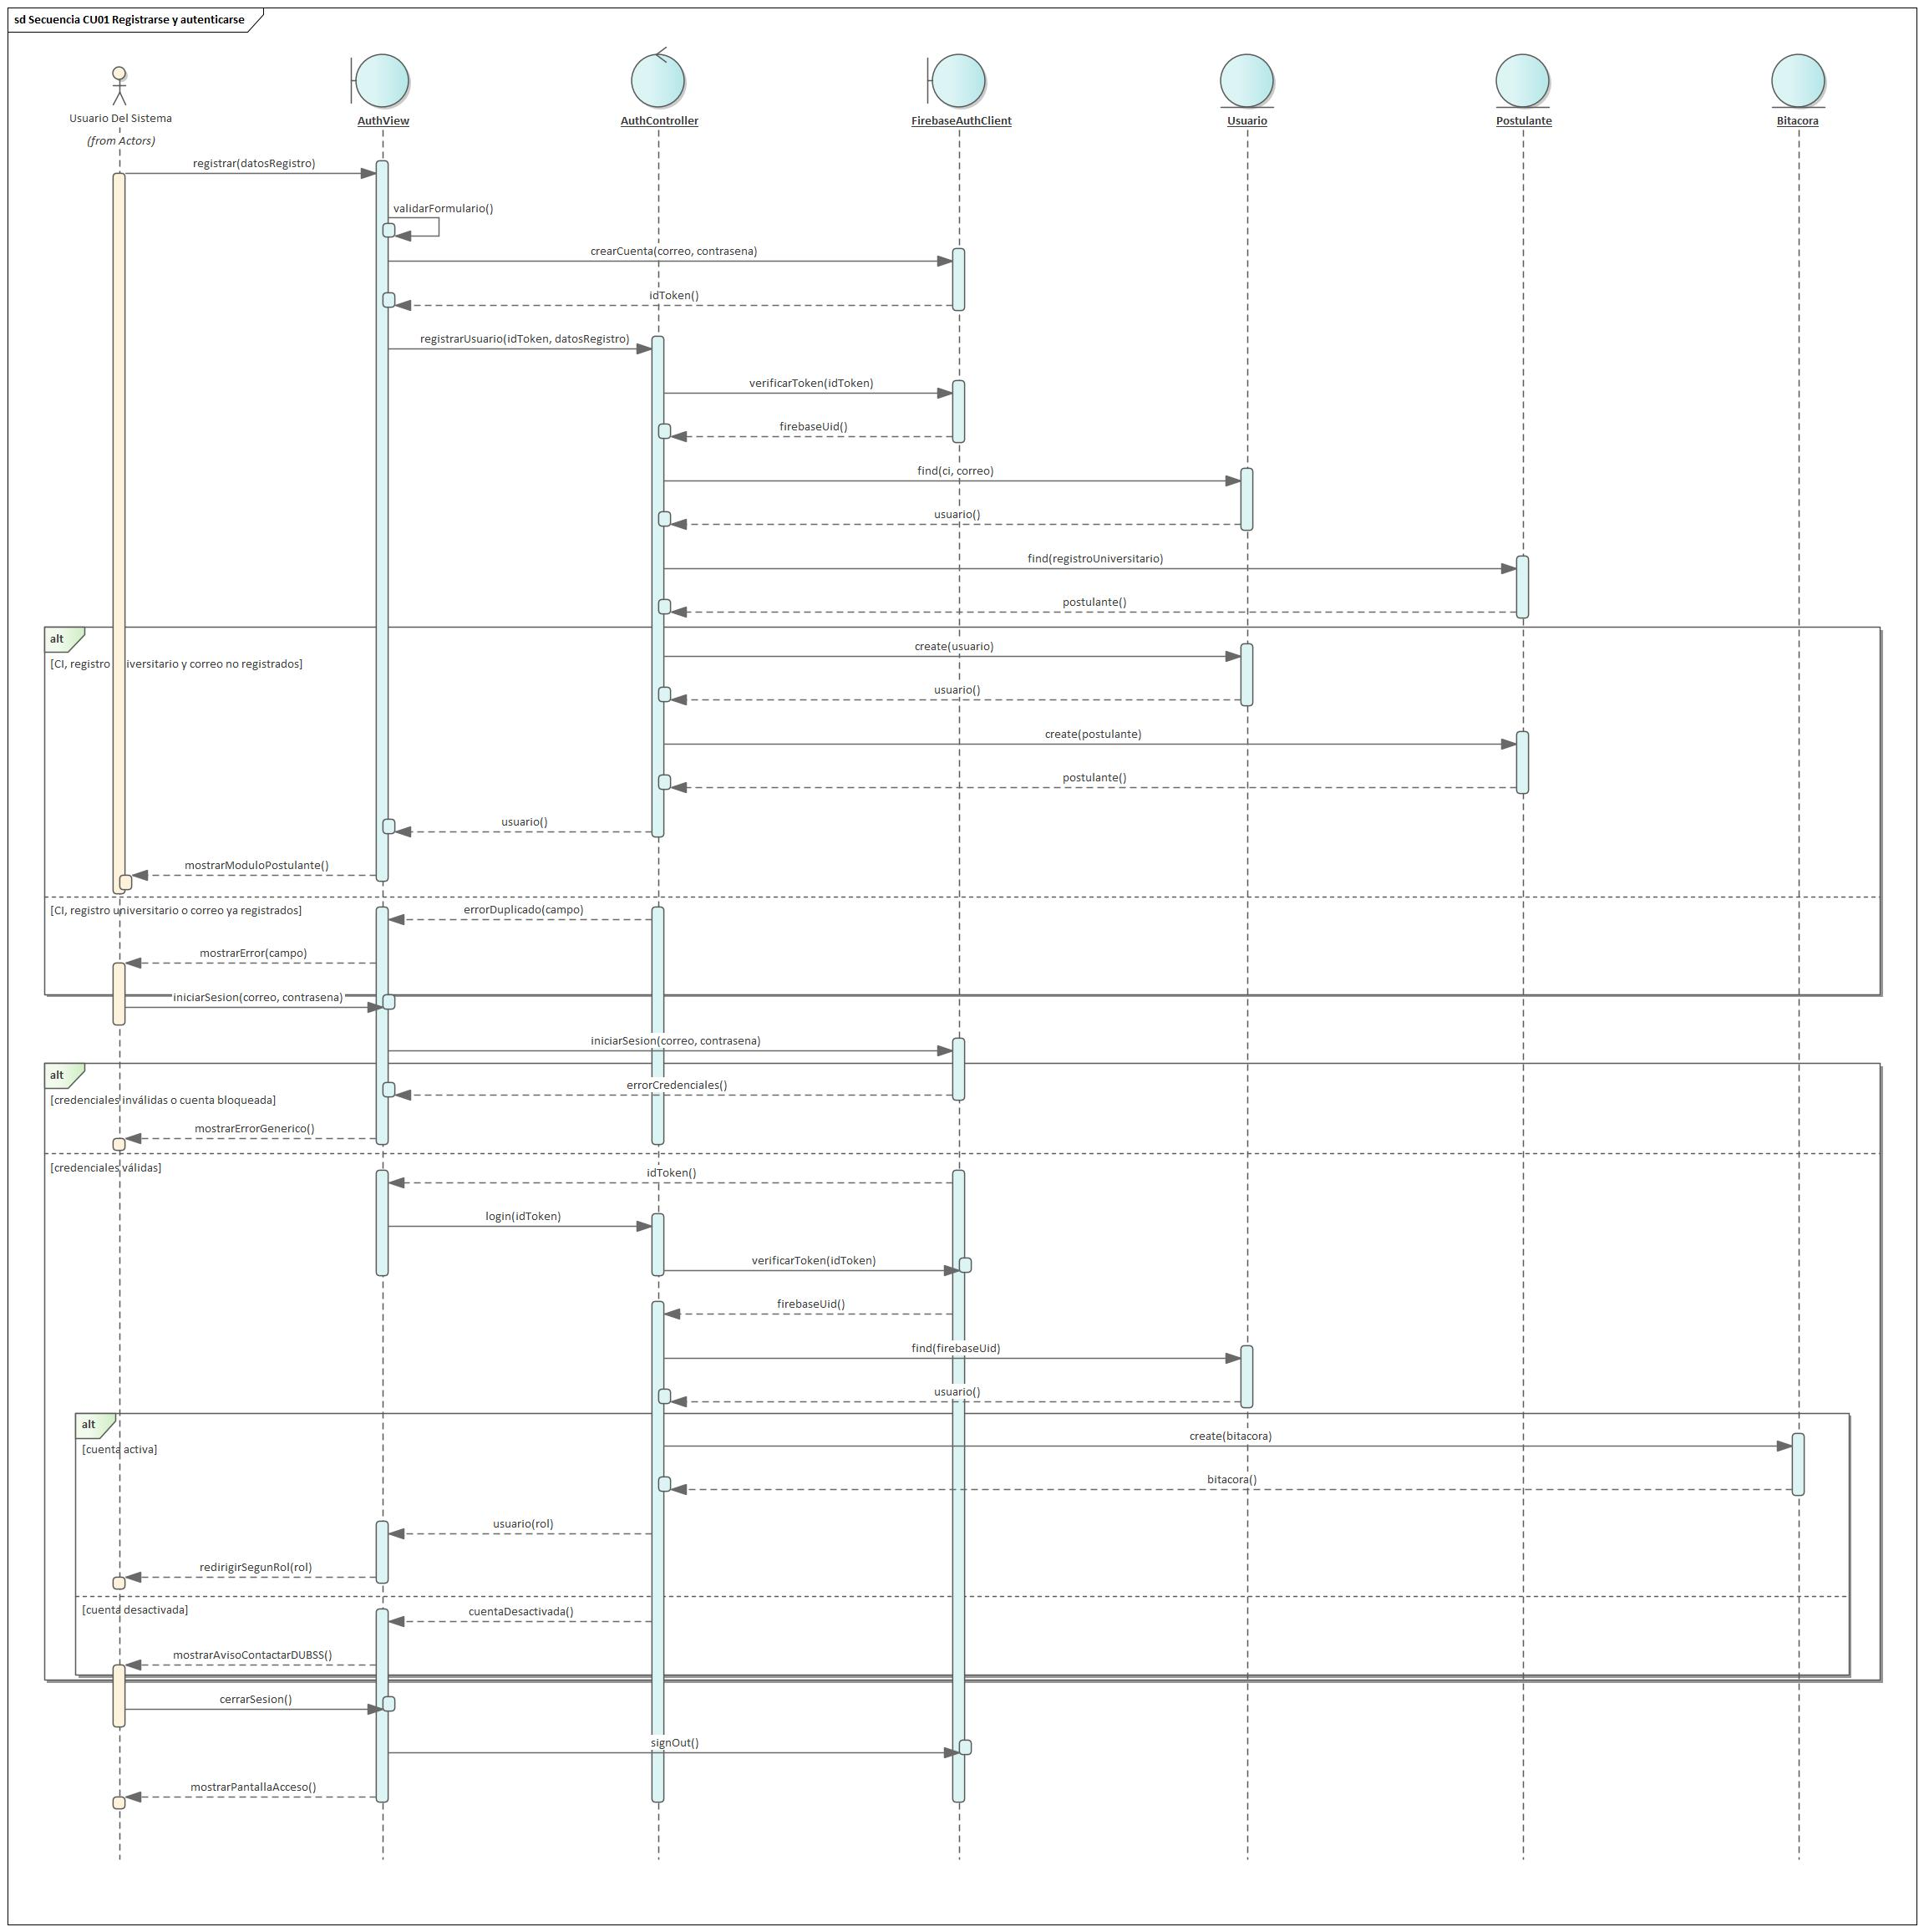
\includegraphics[width=\textwidth,height=0.75\textheight,keepaspectratio]{images/121_Secuencia_CU01_Registrarse_Autenticarse.jpg}

\smallskip
\noindent\raggedright\textit{Nota.} Elaboración propia.
\end{figure}

En el registro, el cliente envía los datos al backend; \textit{AuthController} comprueba que el CI, el registro universitario y el correo electrónico no existan, crea el \textit{Usuario} con el rol Postulante y la contraseña almacenada como hash, crea su perfil de \textit{Postulante} (con registro universitario y teléfono), abre la \textit{Sesion}, anota en la bitácora el registro y el inicio de sesión, y devuelve el token de acceso, el token de renovación y el usuario; si alguno de esos datos ya existe, informa el campo en conflicto y no crea la cuenta. En el inicio de sesión, el controlador busca al \textit{Usuario} por su correo electrónico; si las credenciales no son válidas o la cuenta está bloqueada, actualiza el contador de intentos fallidos y el bloqueo y responde con un mismo mensaje de error. Si son válidas y la cuenta está activa, abre la \textit{Sesion}, anota el acceso en la bitácora y devuelve los tokens y el usuario con su rol, según el cual se redirige al módulo correspondiente; si la cuenta está desactivada, niega el acceso e indica que debe comunicarse con la DUBSS. Cuando el token de acceso vence, el cliente solicita su renovación con el token de renovación: el controlador busca la \textit{Sesion} por el hash del token, la revoca y crea una nueva con un token de renovación nuevo; si la sesión no es válida, el usuario vuelve a la pantalla de acceso. Para cerrar sesión, el controlador revoca la \textit{Sesion} del dispositivo, sin afectar las de otros dispositivos. La contraseña (mínimo de 6 caracteres) se almacena solo como hash y el bloqueo tras 5 intentos fallidos consecutivos lo aplica el propio sistema.


\Needspace{0.9\textheight}
\subsubsection{7.4.2. Diseñar CU-02 Enviar postulación a Beca Comedor}\label{sec:cap7_disenar_cu02}

La Figura~\ref{fig:secuencia_cu02} presenta el diagrama de secuencia del CU-02.

\begin{figure}[H]
\caption{Diagrama de secuencia del CU-02 Enviar postulación a Beca Comedor}
\label{fig:secuencia_cu02}
\centering
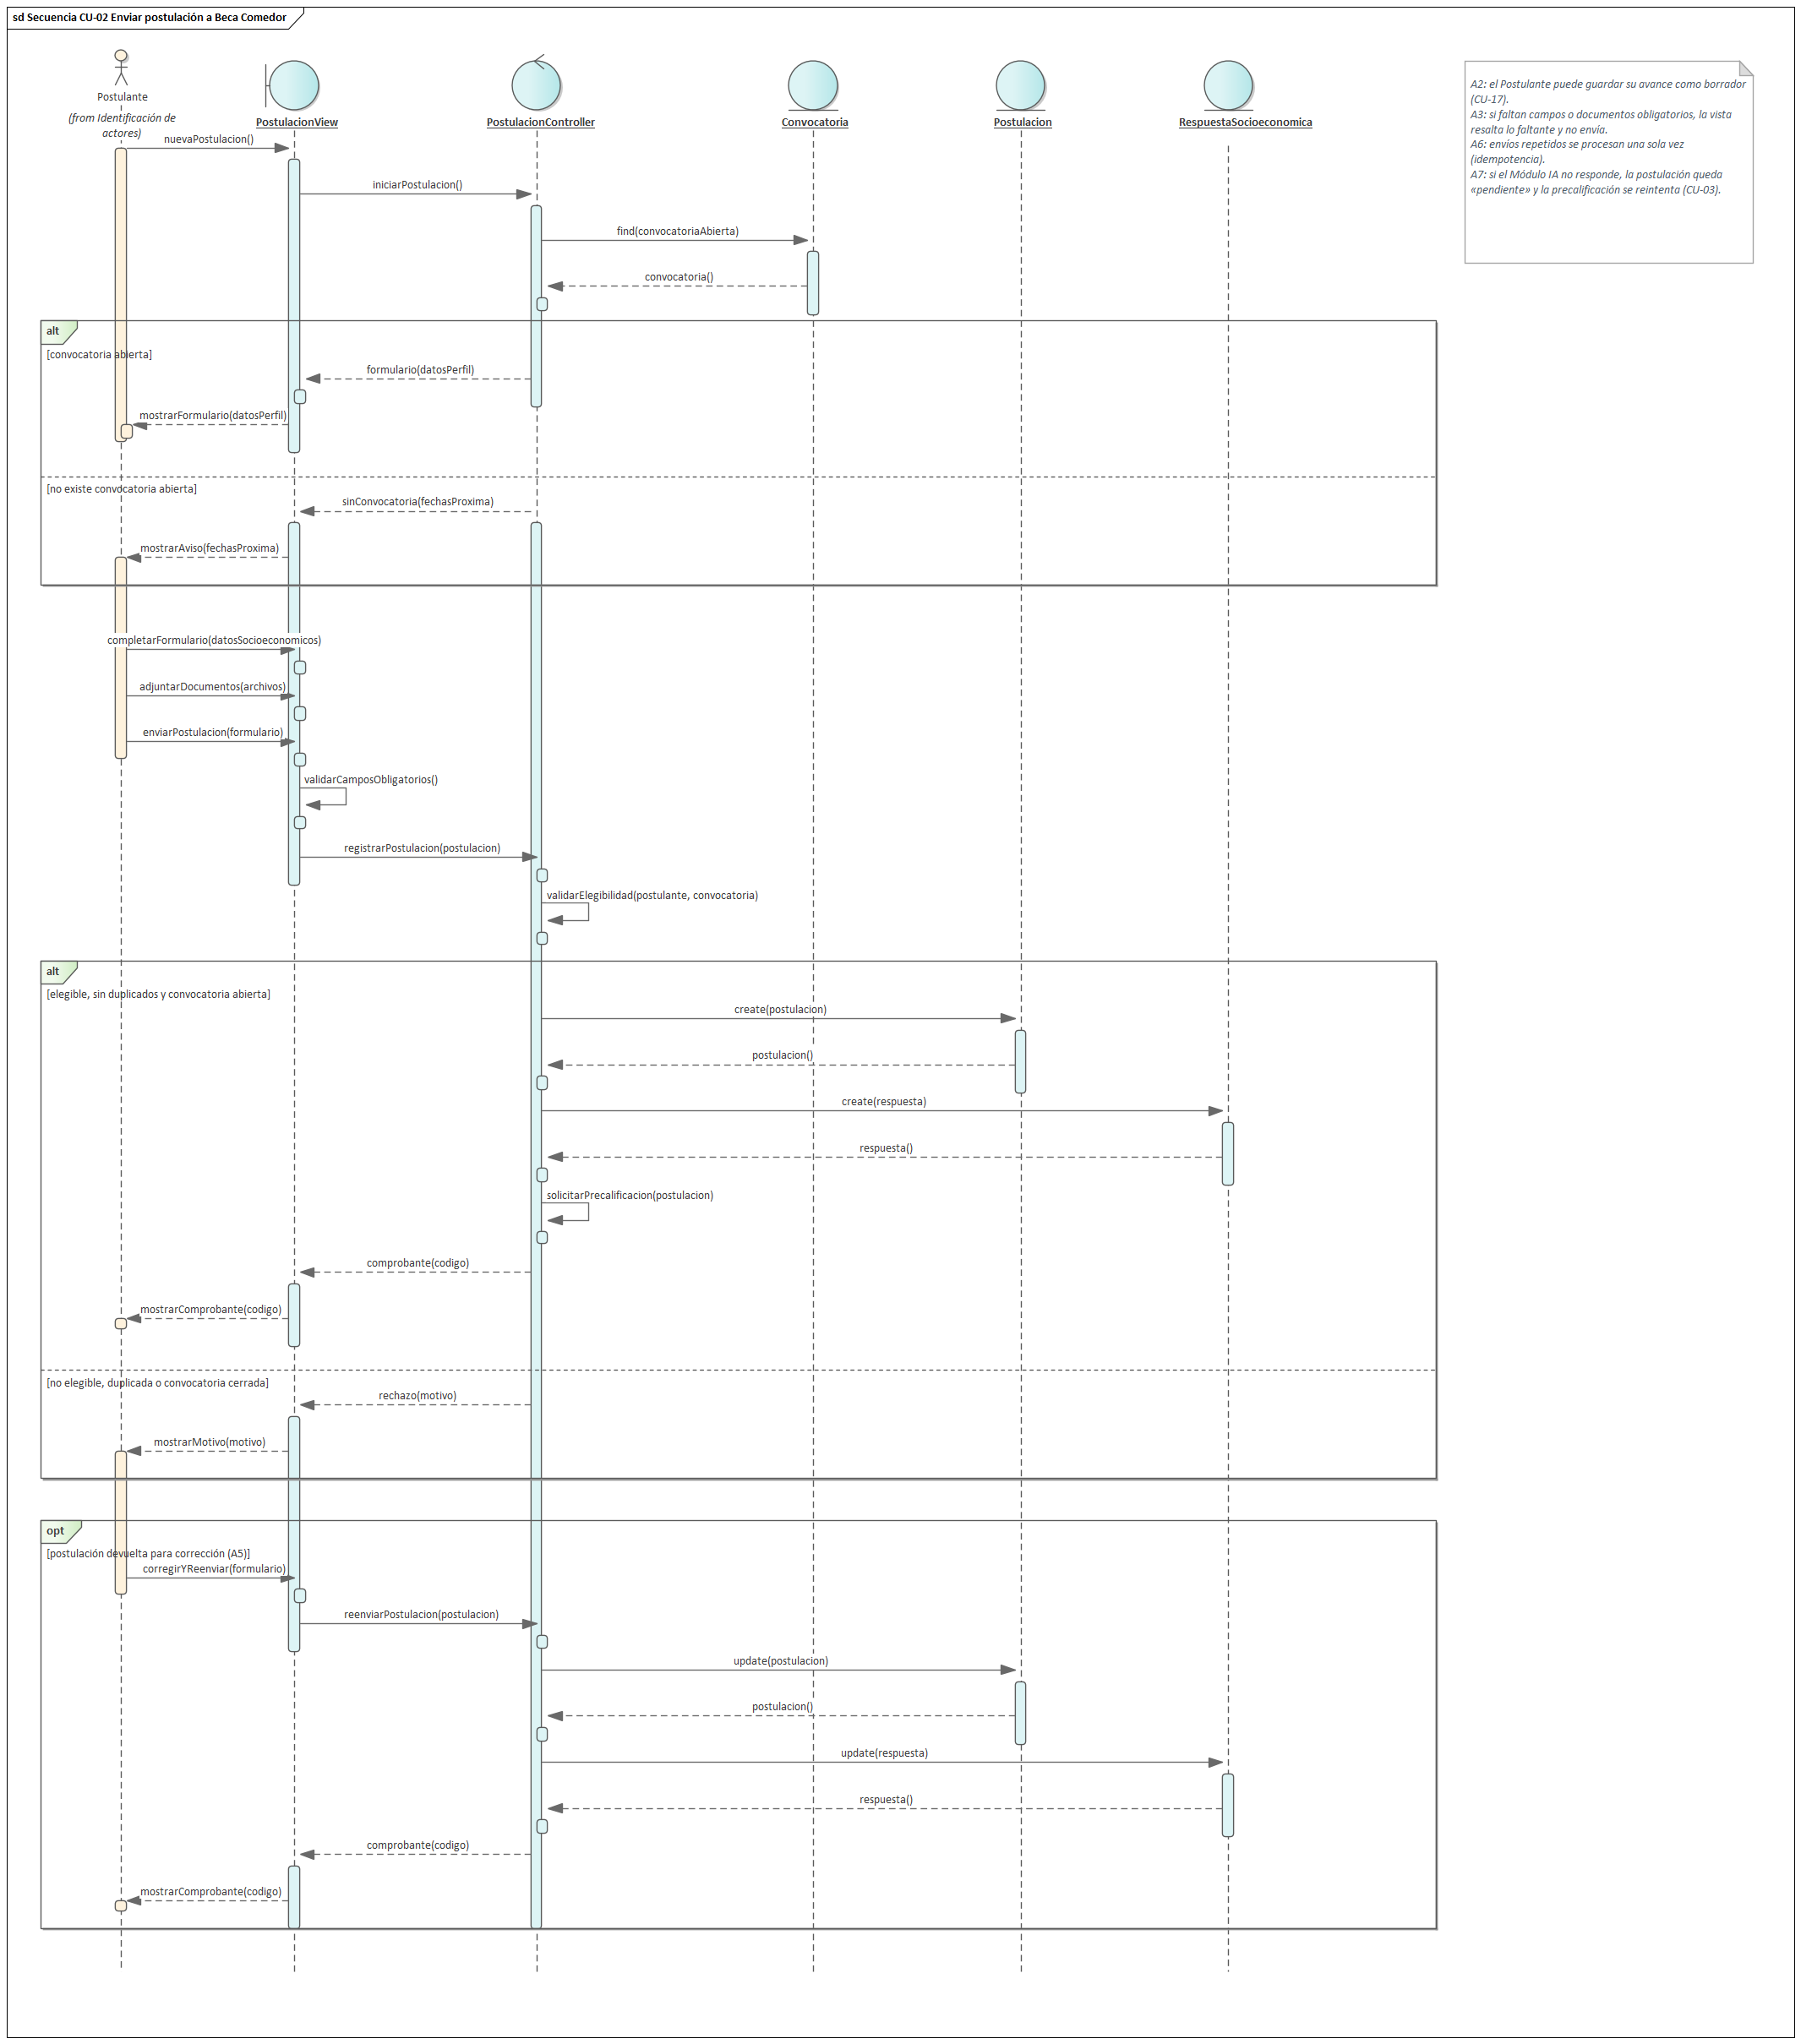
\includegraphics[width=\textwidth,height=0.75\textheight,keepaspectratio]{images/122_Secuencia_CU02_Enviar_Postulacion_Beca_Comedor.png}

\smallskip
\noindent\raggedright\textit{Nota.} Elaboración propia.
\end{figure}


\Needspace{0.9\textheight}
\subsubsection{7.4.3. Diseñar CU-03 Precalificar postulación con Inteligencia Artificial}\label{sec:cap7_disenar_cu03}

La Figura~\ref{fig:secuencia_cu03} presenta el diagrama de secuencia del CU-03.

\begin{figure}[H]
\caption{Diagrama de secuencia del CU-03 Precalificar postulación con Inteligencia Artificial}
\label{fig:secuencia_cu03}
\centering
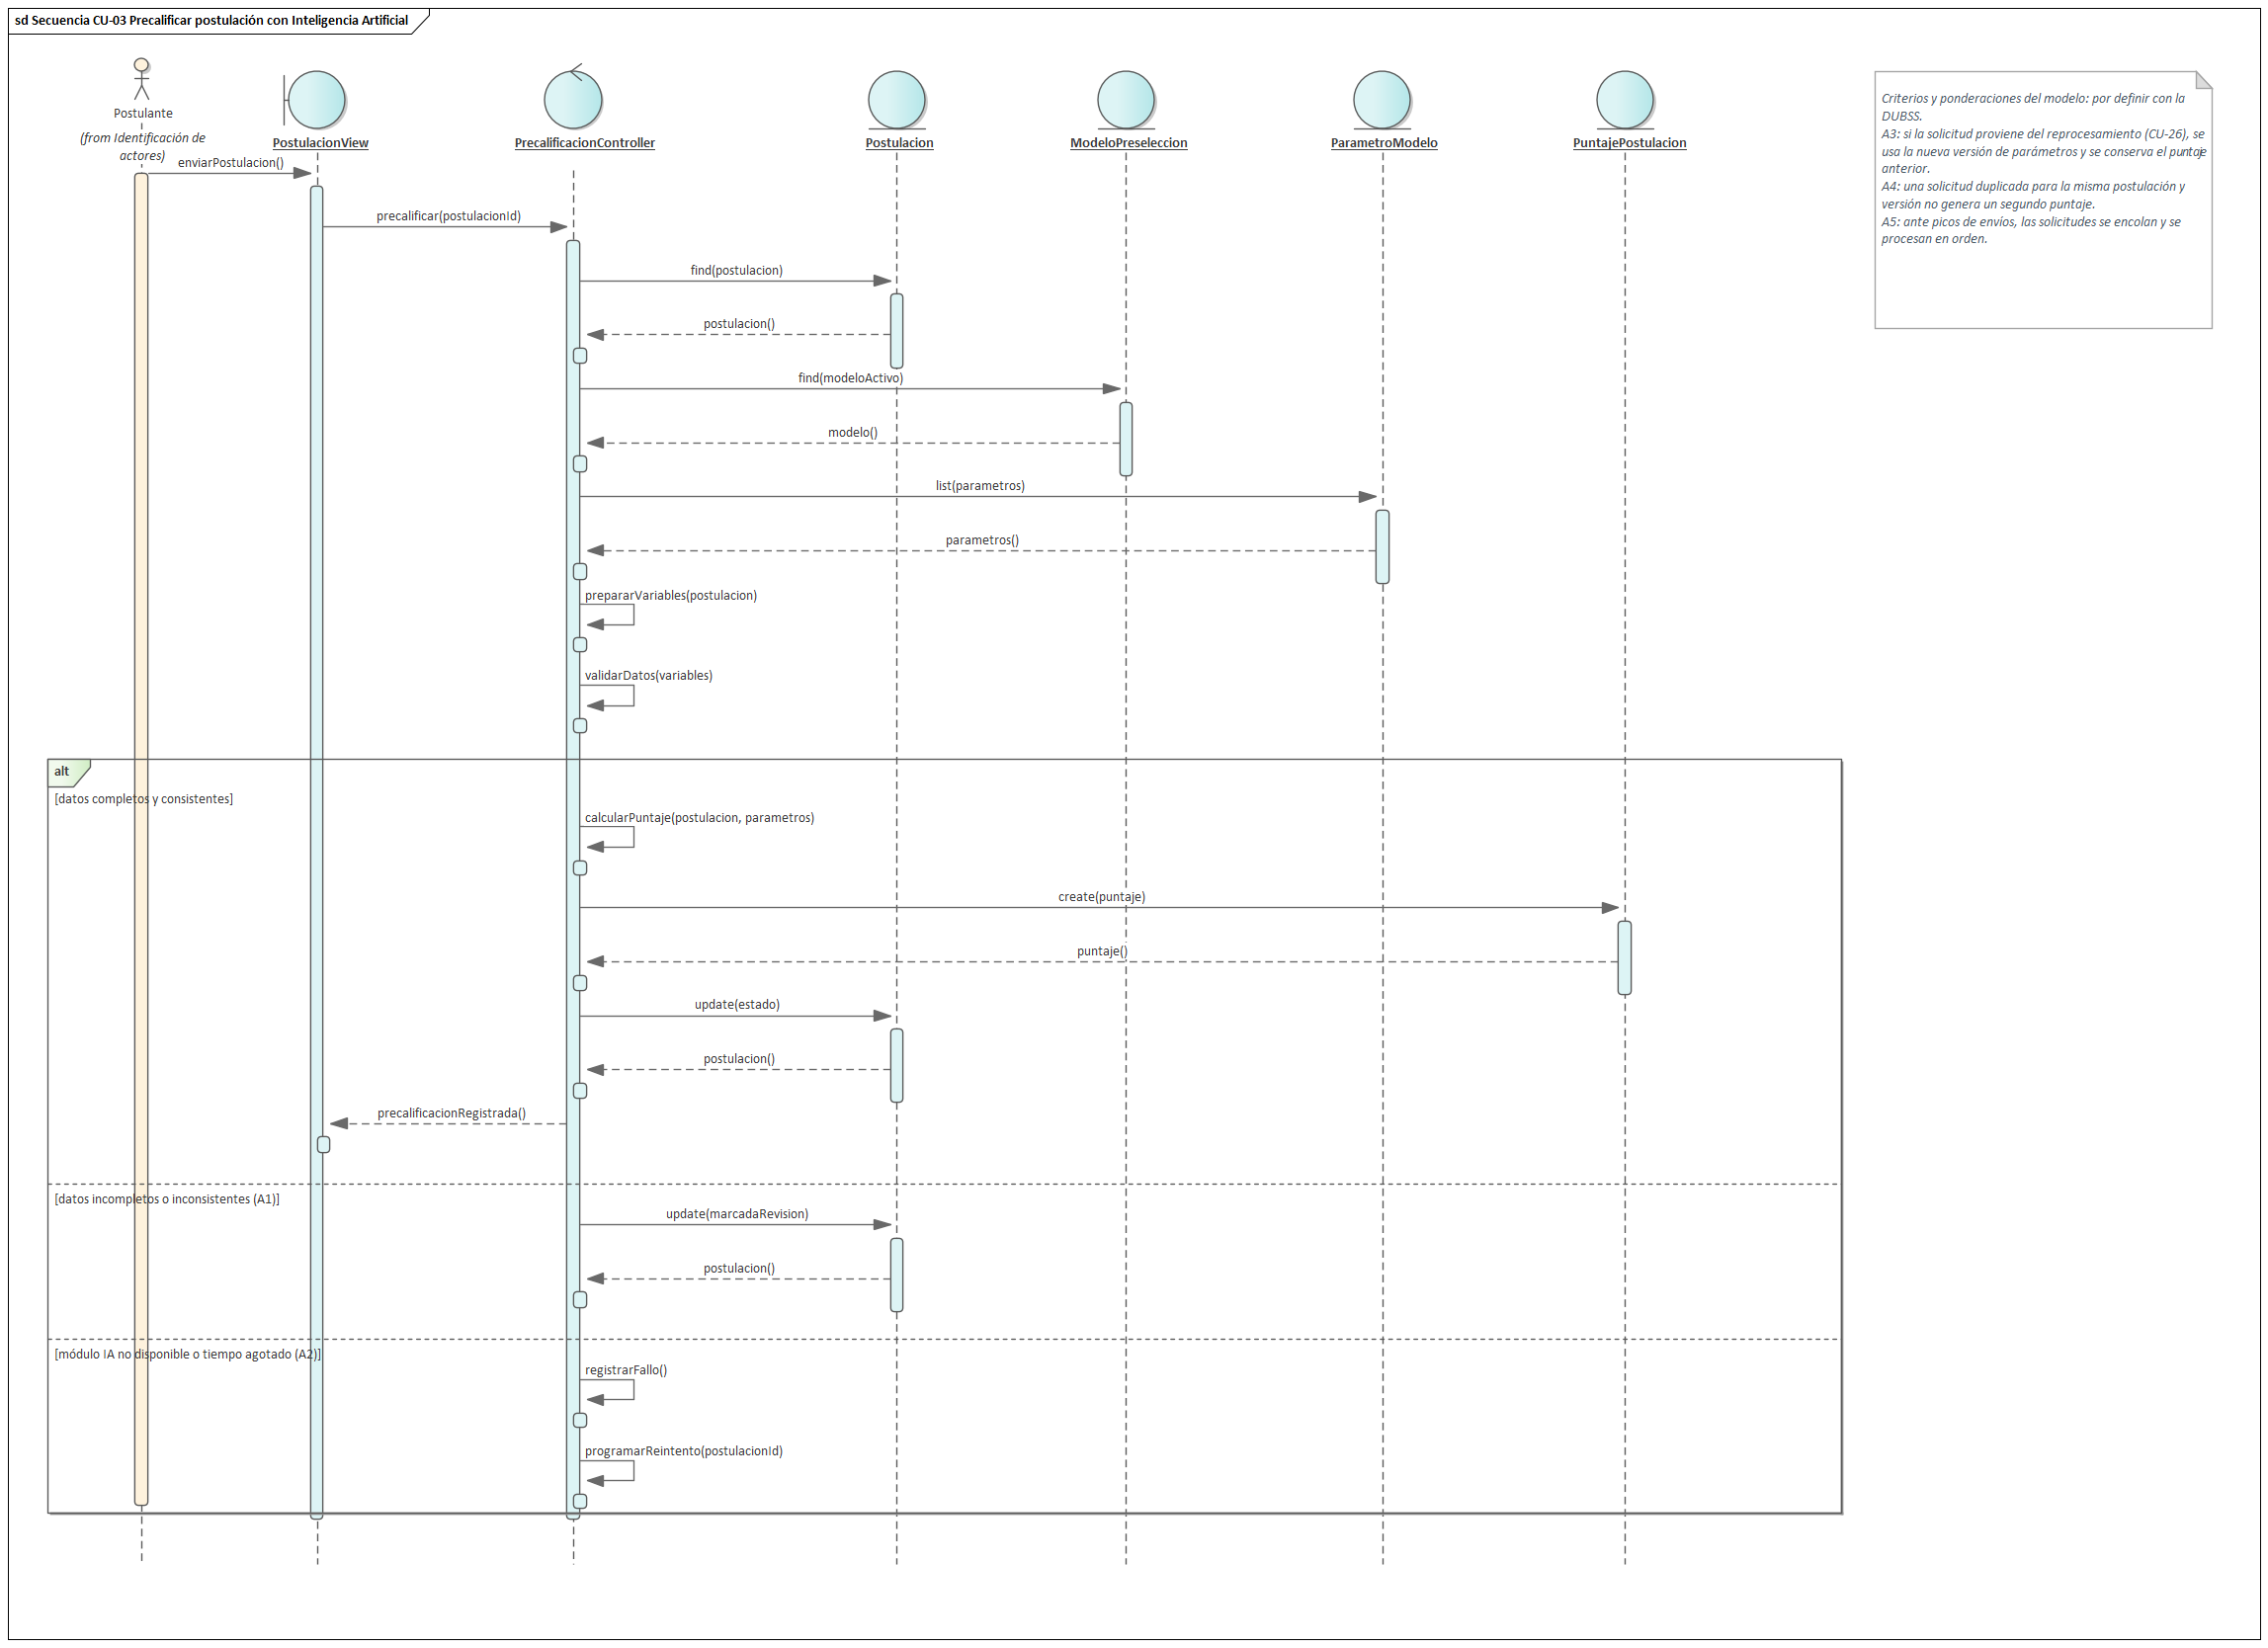
\includegraphics[width=\textwidth,height=0.75\textheight,keepaspectratio]{images/123_Secuencia_CU03_Precalificar_Postulacion_IA.png}

\smallskip
\noindent\raggedright\textit{Nota.} Elaboración propia.
\end{figure}


\Needspace{0.9\textheight}
\subsubsection{7.4.4. Diseñar CU-04 Consultar estado de postulación}\label{sec:cap7_disenar_cu04}

La Figura~\ref{fig:secuencia_cu04} presenta el diagrama de secuencia del CU-04.

\begin{figure}[H]
\caption{Diagrama de secuencia del CU-04 Consultar estado de postulación}
\label{fig:secuencia_cu04}
\centering
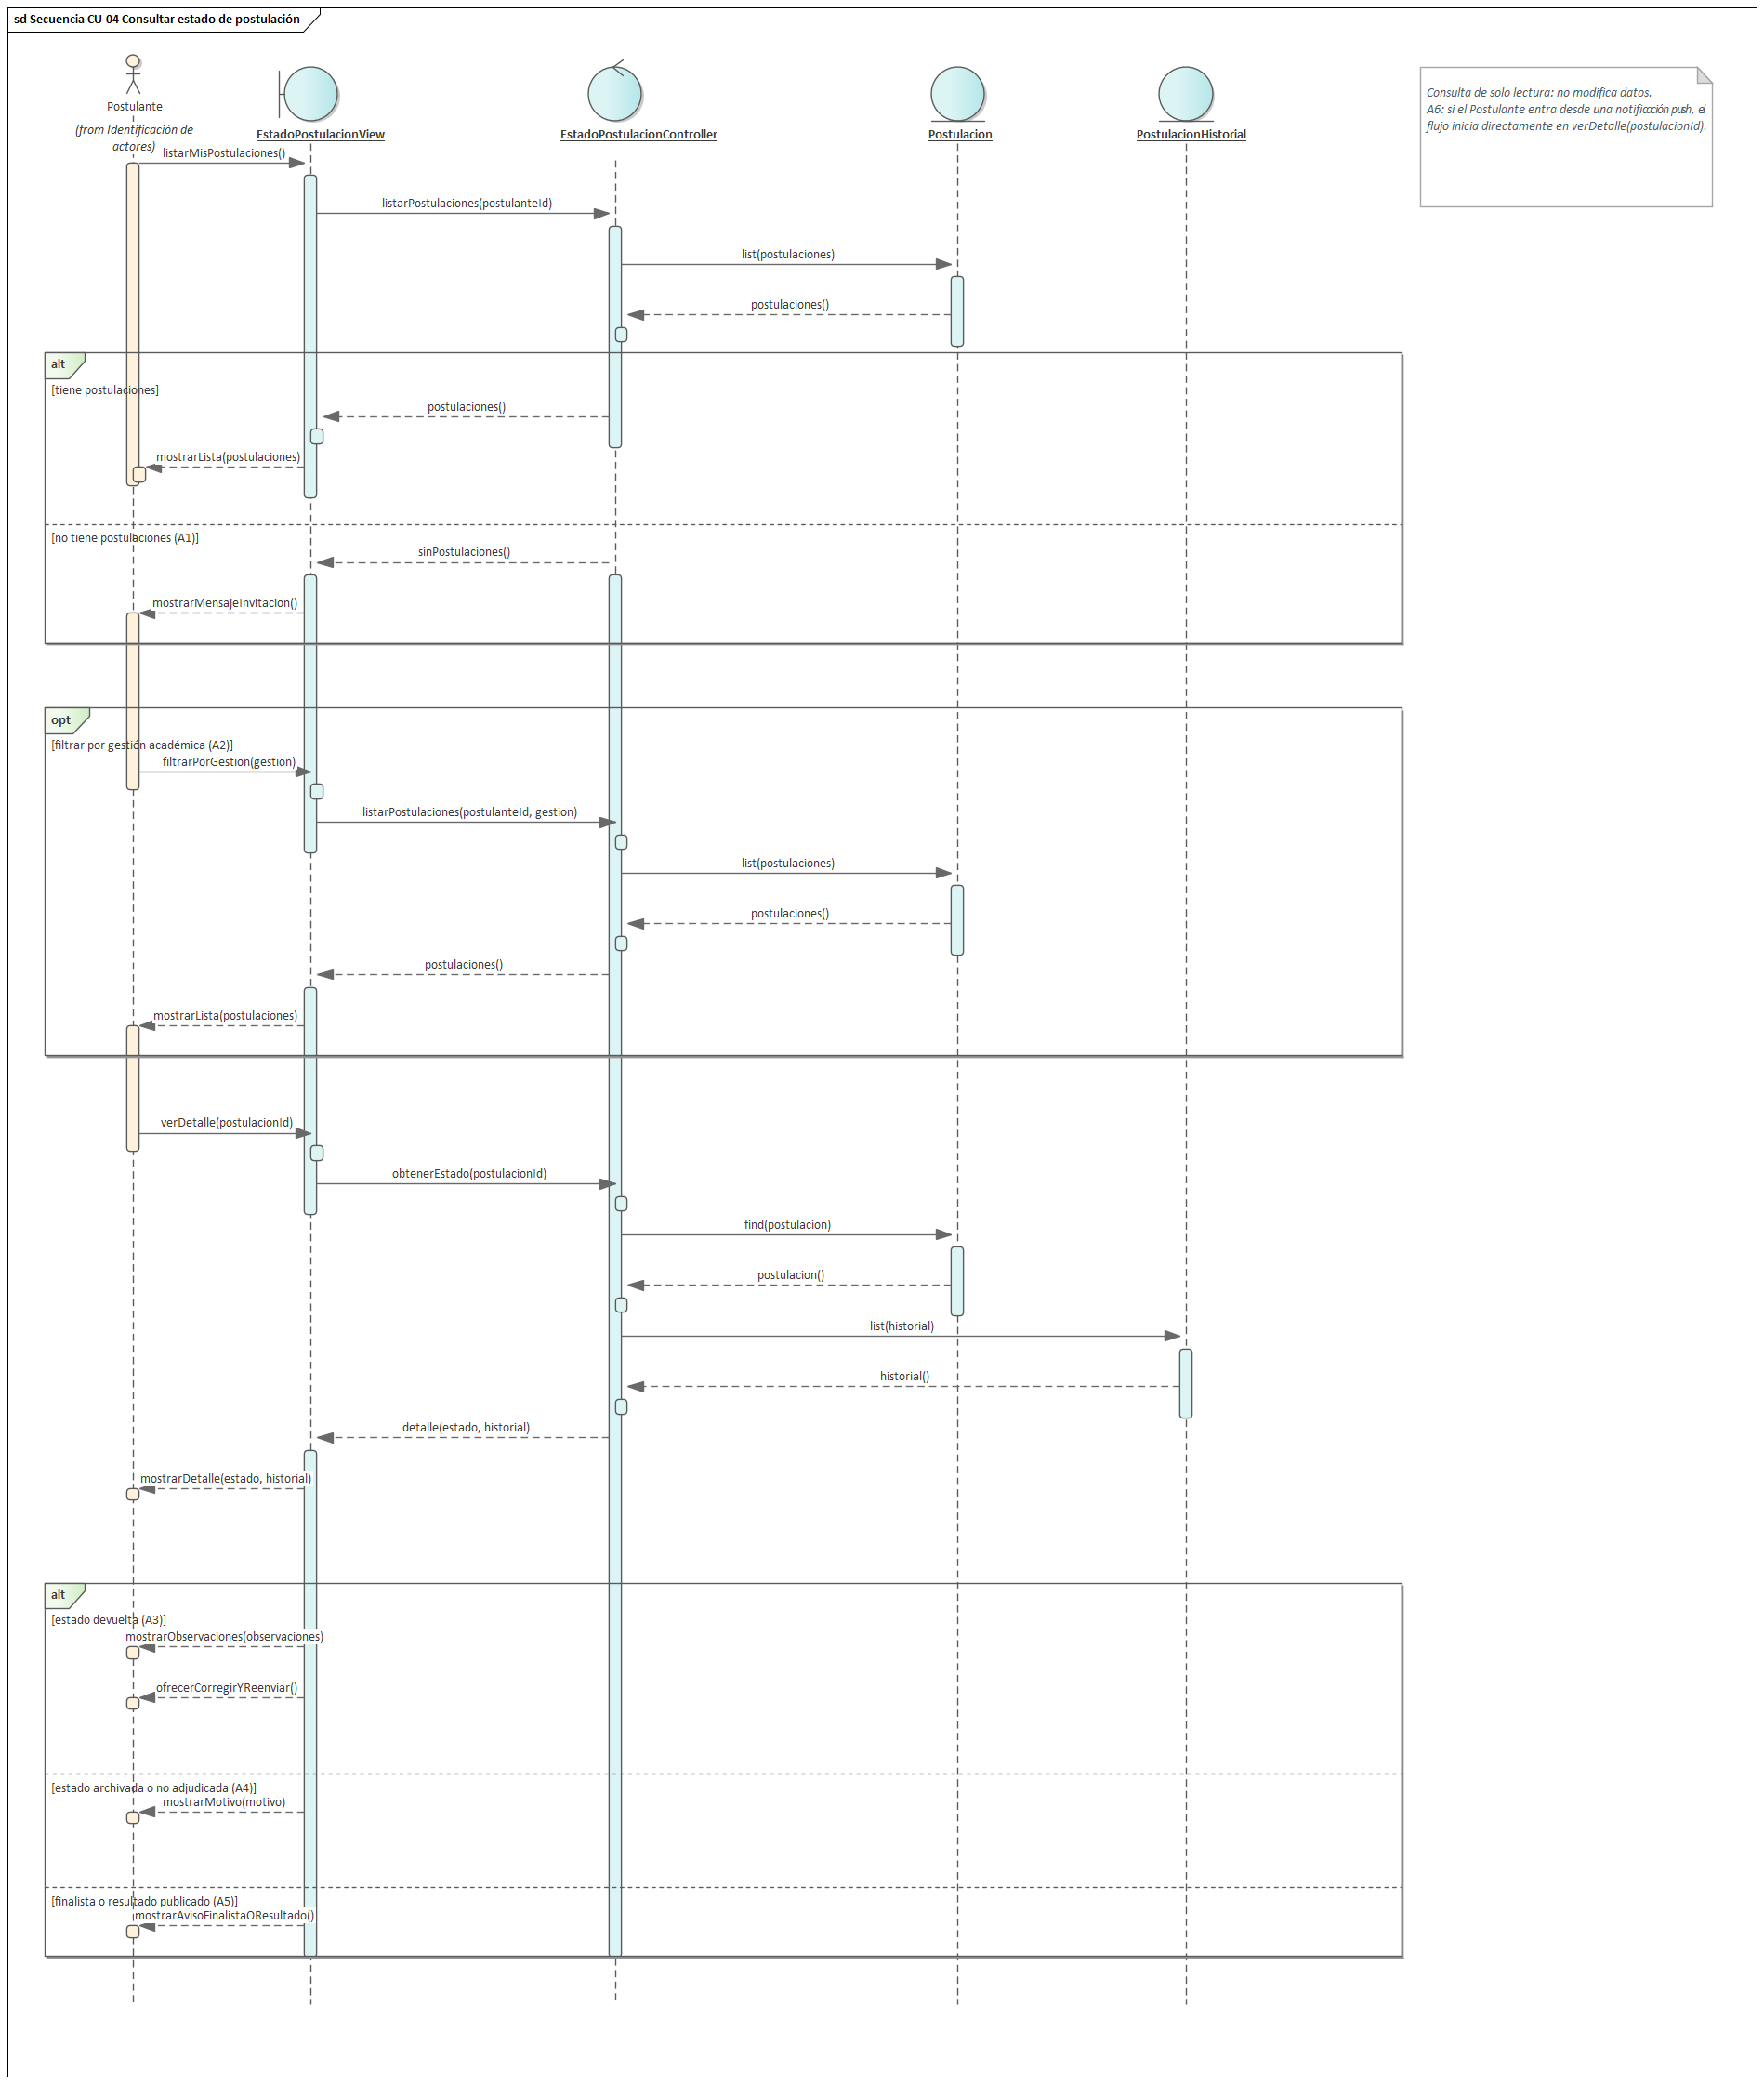
\includegraphics[width=\textwidth,height=0.75\textheight,keepaspectratio]{images/124_Secuencia_CU04_Consultar_Estado_Postulacion.png}

\smallskip
\noindent\raggedright\textit{Nota.} Elaboración propia.
\end{figure}


\Needspace{0.9\textheight}
\subsubsection{7.4.5. Diseñar CU-05 Auditar y adjudicar becas}\label{sec:cap7_disenar_cu05}

La Figura~\ref{fig:secuencia_cu05} presenta el diagrama de secuencia del CU-05.

\begin{figure}[H]
\caption{Diagrama de secuencia del CU-05 Auditar y adjudicar becas}
\label{fig:secuencia_cu05}
\centering
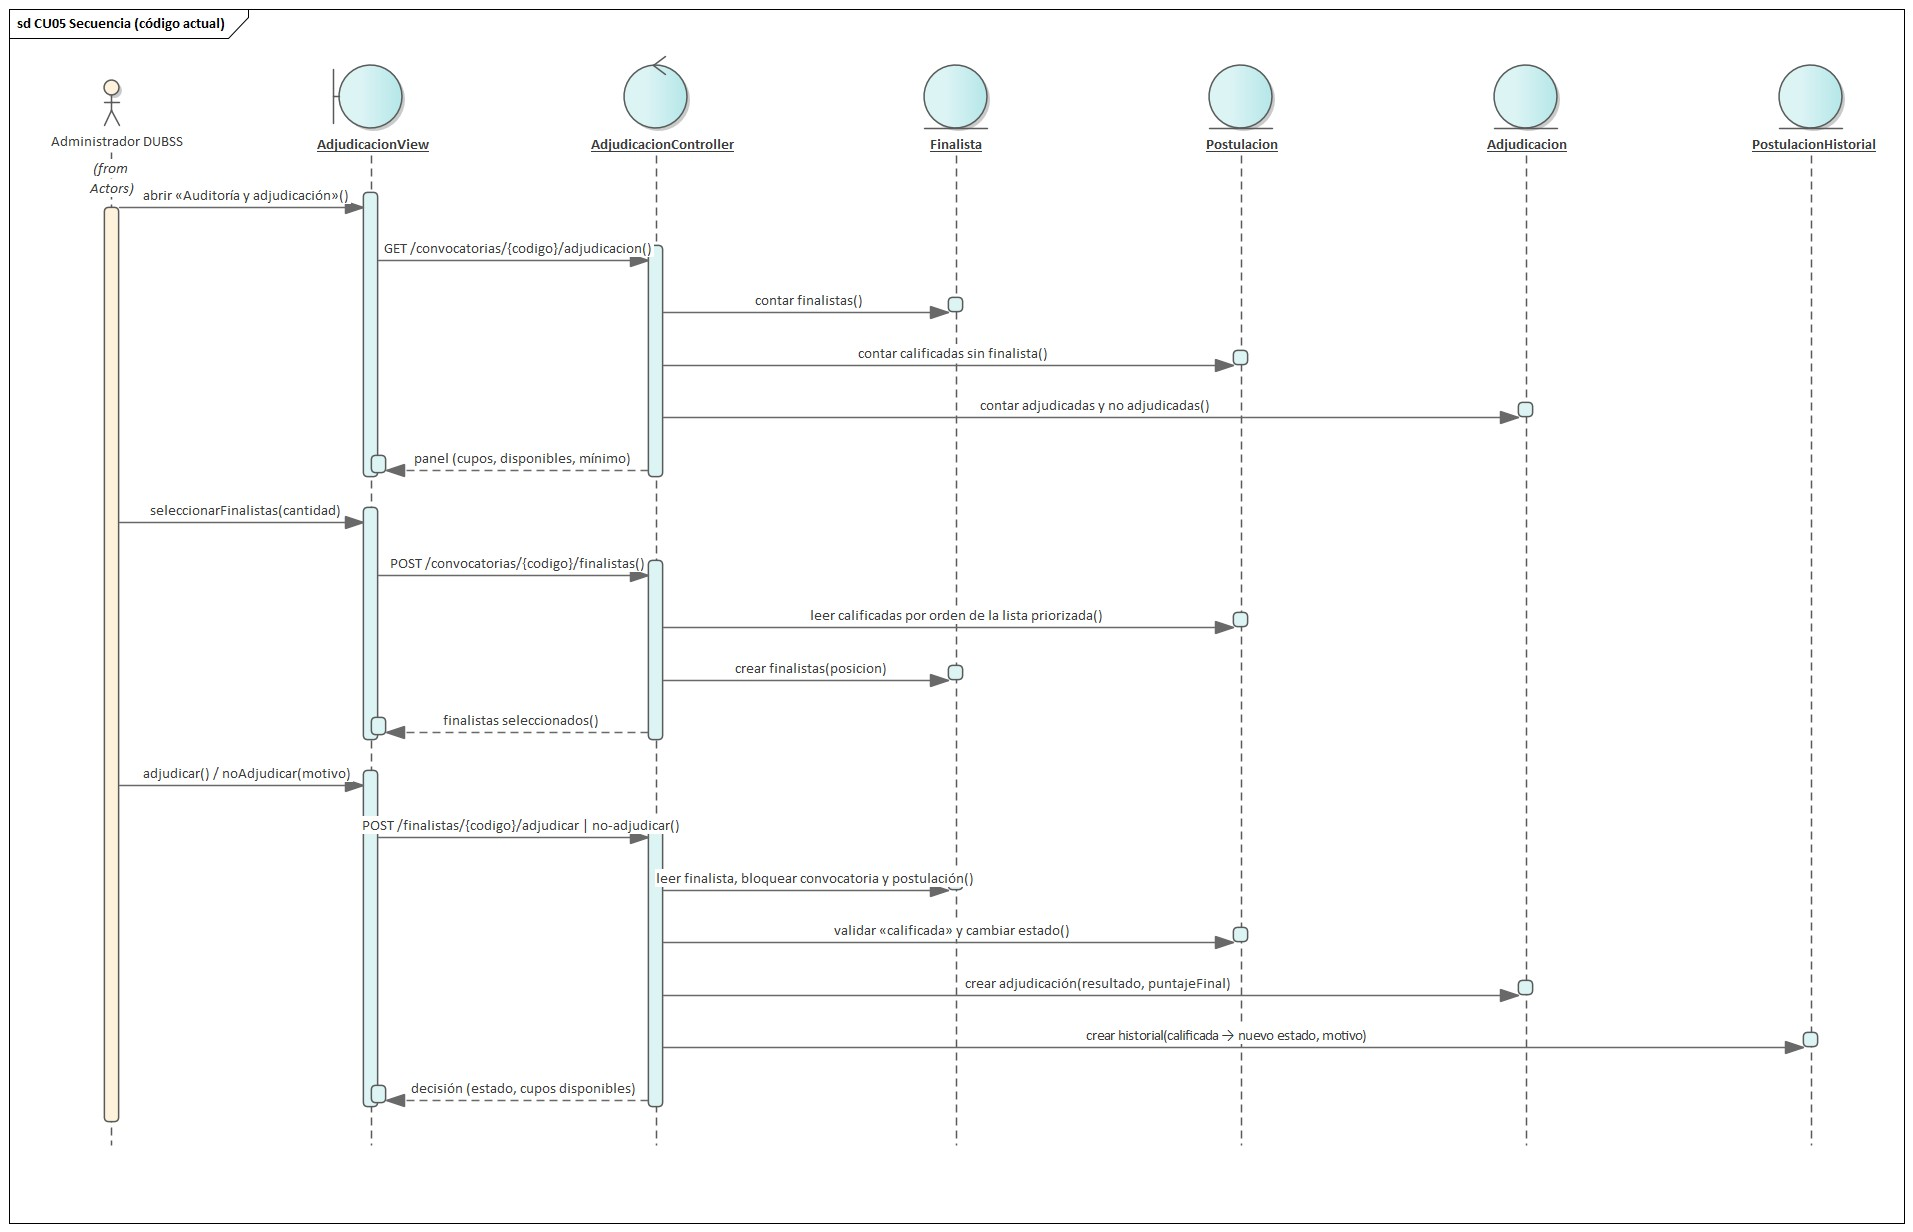
\includegraphics[width=\textwidth,height=0.75\textheight,keepaspectratio]{images/092_Secuencia_CU05_Auditar_Adjudicar_Becas.jpg}

\smallskip
\noindent\raggedright\textit{Nota.} Elaboración propia.
\end{figure}


\Needspace{0.9\textheight}
\subsubsection{7.4.6. Diseñar CU-06 Visualizar lista priorizada de postulantes}\label{sec:cap7_disenar_cu06}

La Figura~\ref{fig:secuencia_cu06} presenta el diagrama de secuencia del CU-06.

\begin{figure}[H]
\caption{Diagrama de secuencia del CU-06 Visualizar lista priorizada de postulantes}
\label{fig:secuencia_cu06}
\centering
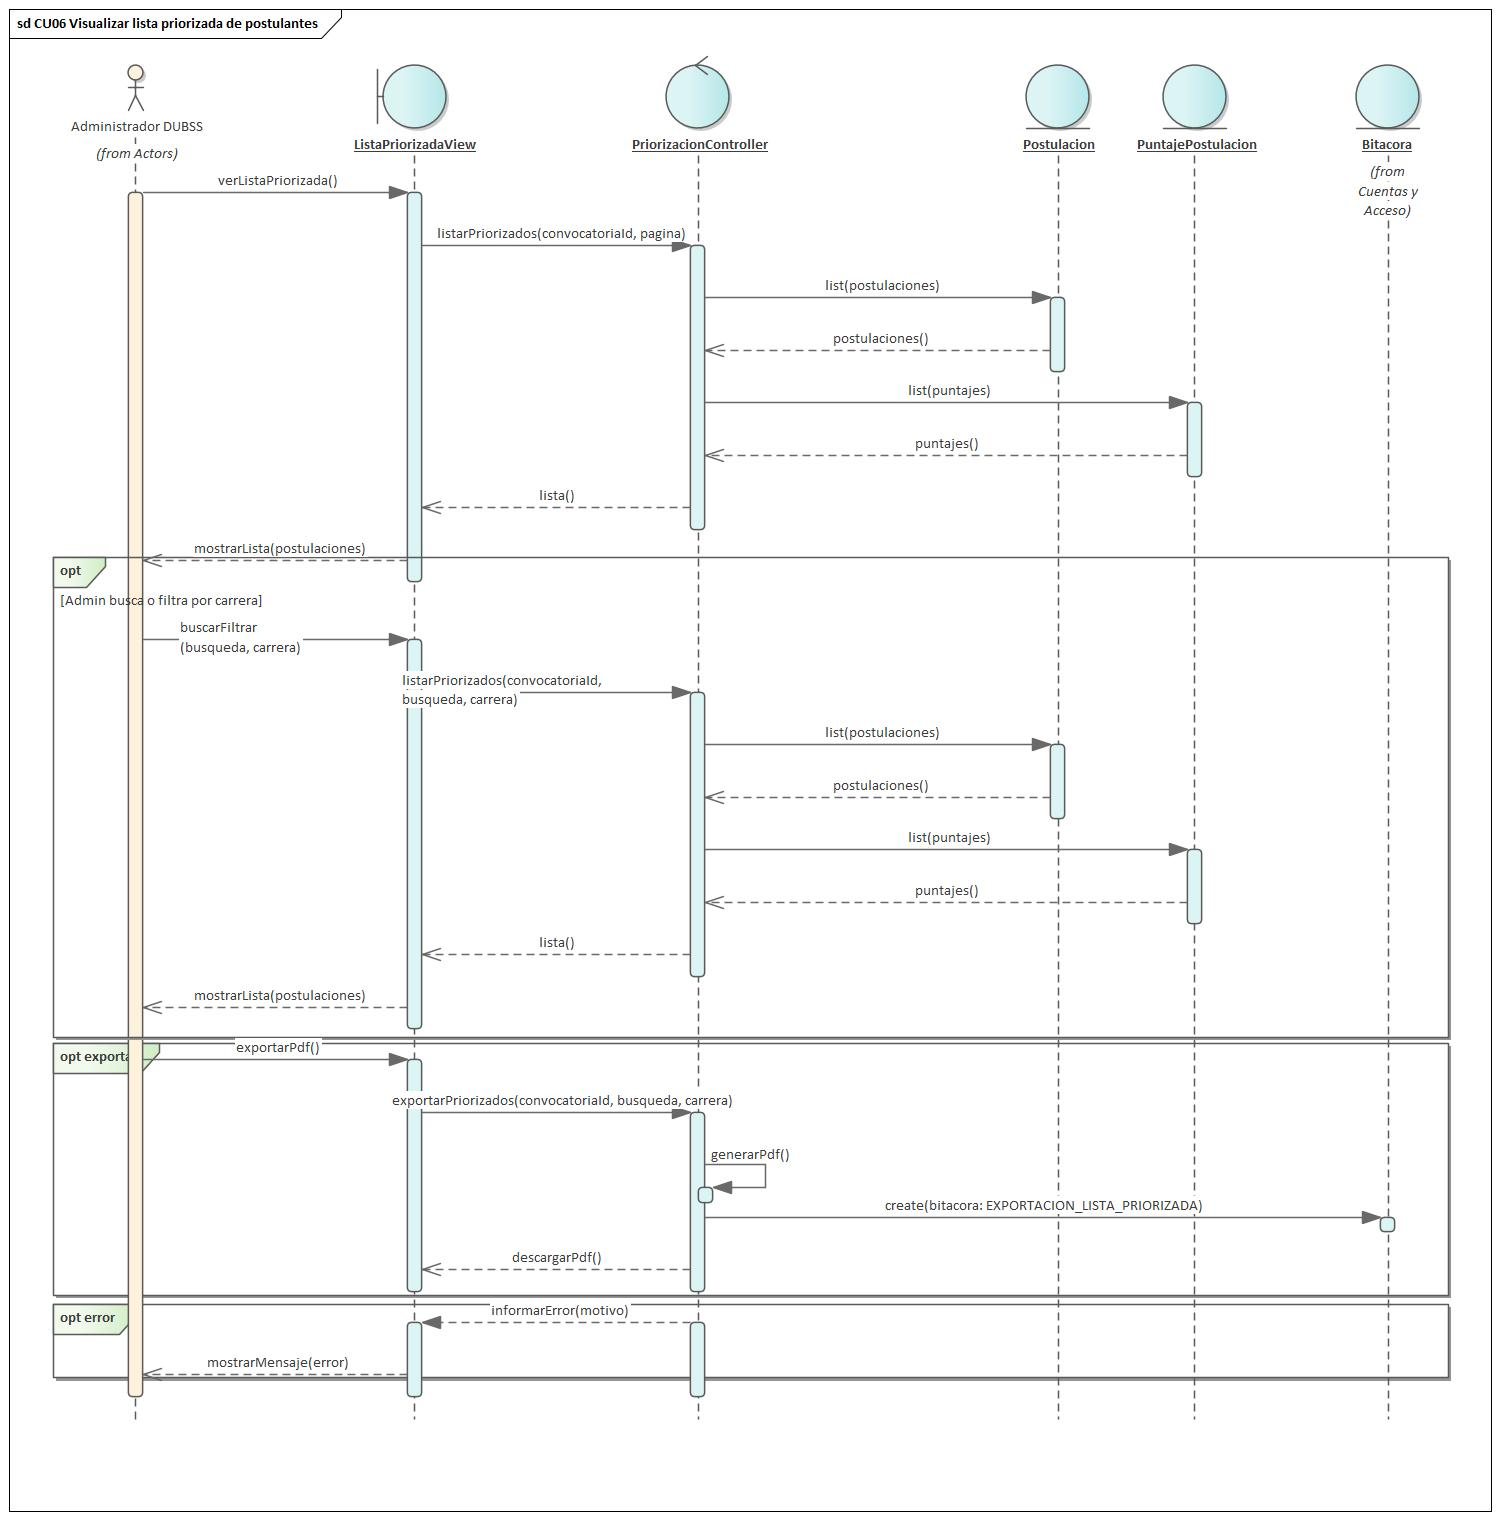
\includegraphics[width=\textwidth,height=0.75\textheight,keepaspectratio]{images/093_Secuencia_CU06_Visualizar_Lista_Priorizada_Postulantes.jpg}

\smallskip
\noindent\raggedright\textit{Nota.} Elaboración propia.
\end{figure}


\Needspace{0.9\textheight}
\subsubsection{7.4.7. Diseñar CU-07 Auditar expediente finalista}\label{sec:cap7_disenar_cu07}

La Figura~\ref{fig:secuencia_cu07} presenta el diagrama de secuencia del CU-07.

\begin{figure}[H]
\caption{Diagrama de secuencia del CU-07 Auditar expediente finalista}
\label{fig:secuencia_cu07}
\centering
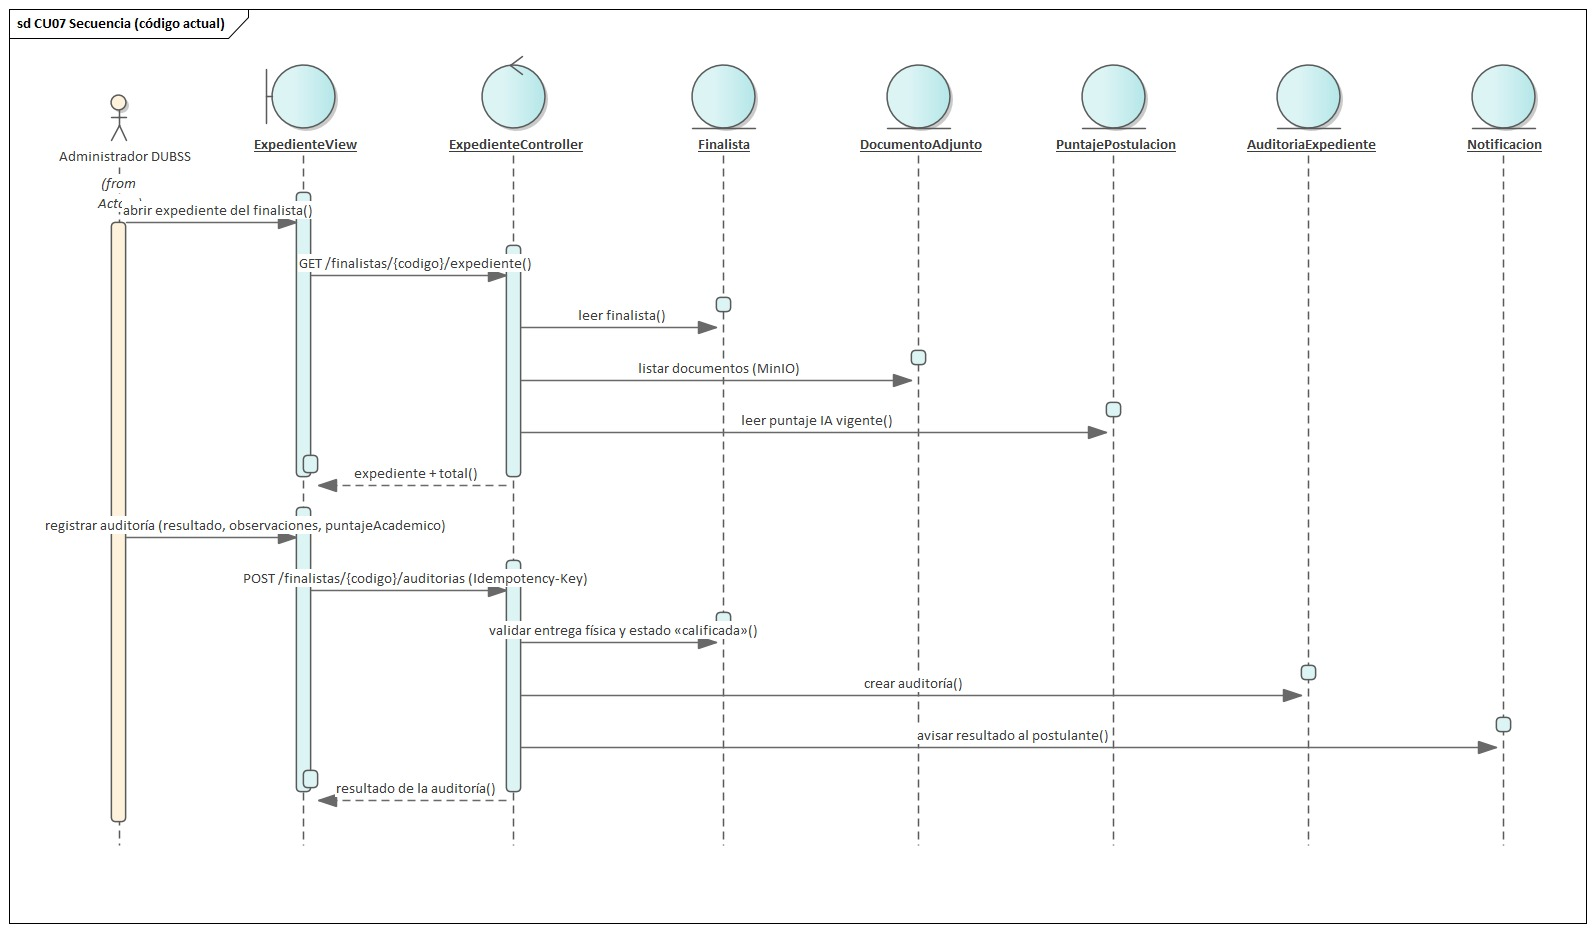
\includegraphics[width=\textwidth,height=0.75\textheight,keepaspectratio]{images/094_Secuencia_CU07_Auditar_Expediente_Finalista.jpg}

\smallskip
\noindent\raggedright\textit{Nota.} Elaboración propia.
\end{figure}


\Needspace{0.9\textheight}
\subsubsection{7.4.8. Diseñar CU-08 Generar acta de adjudicación}\label{sec:cap7_disenar_cu08}

La Figura~\ref{fig:secuencia_cu08} presenta el diagrama de secuencia del CU-08.

\begin{figure}[H]
\caption{Diagrama de secuencia del CU-08 Generar acta de adjudicación}
\label{fig:secuencia_cu08}
\centering
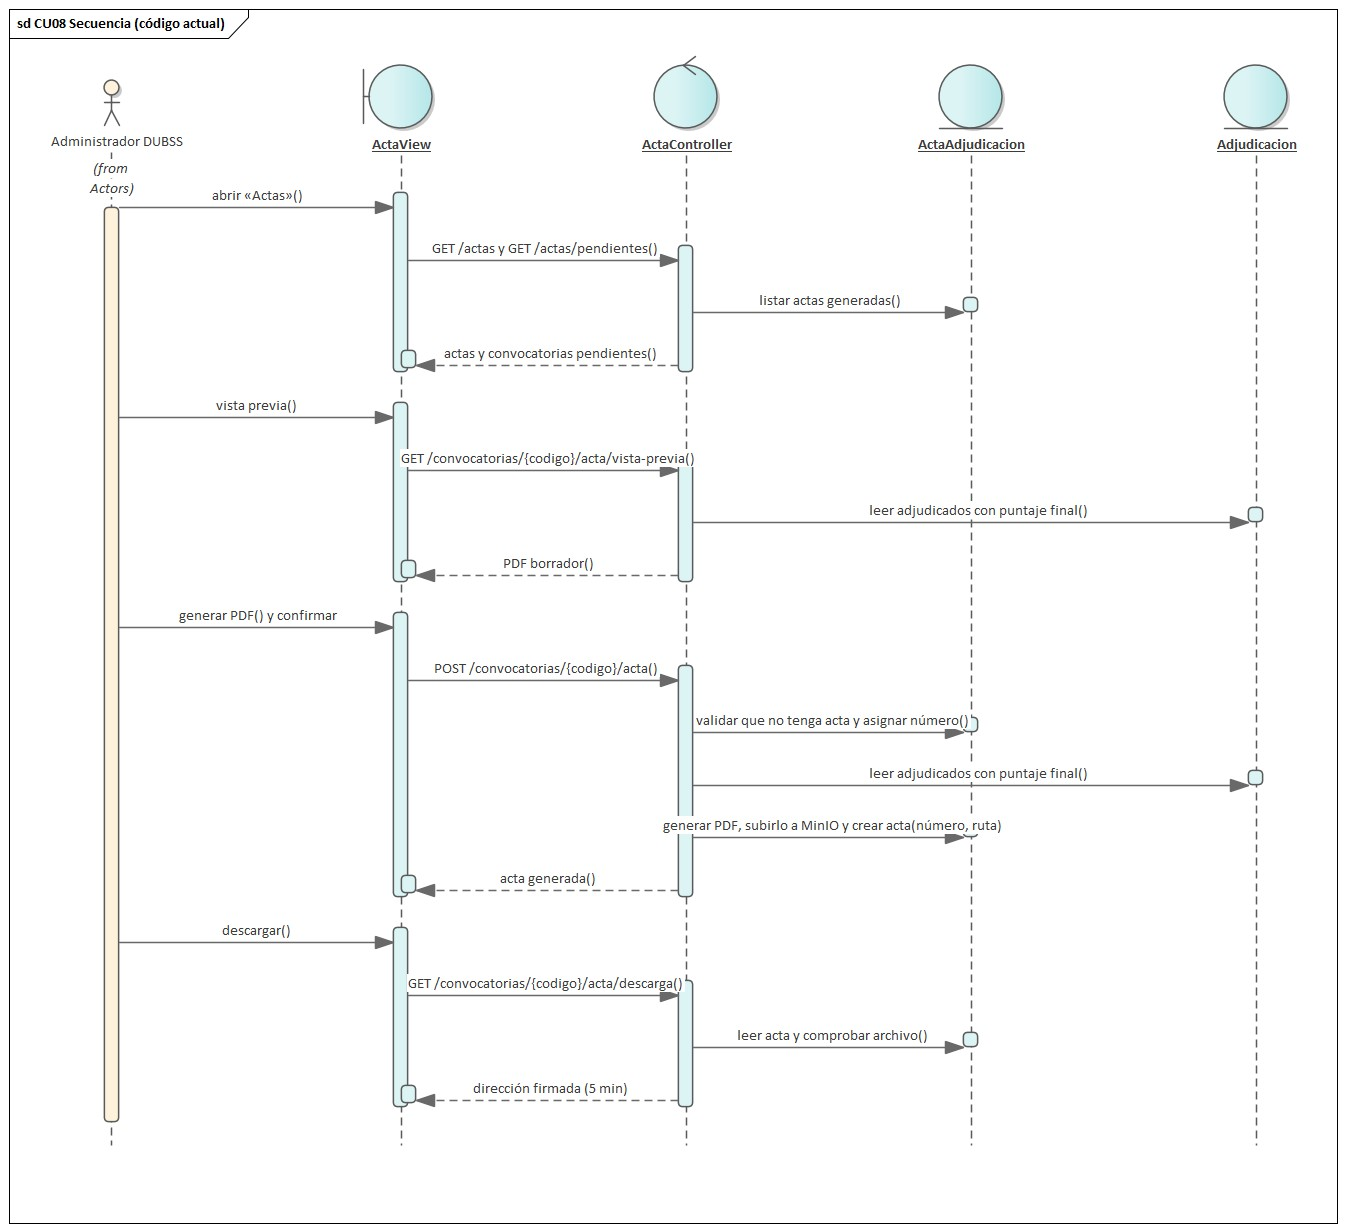
\includegraphics[width=\textwidth,height=0.75\textheight,keepaspectratio]{images/095_Secuencia_CU08_Generar_Acta_Adjudicacion.jpg}

\smallskip
\noindent\raggedright\textit{Nota.} Elaboración propia.
\end{figure}


\Needspace{0.9\textheight}
\subsubsection{7.4.9. Diseñar CU-09 Generar planilla de asistencia}\label{sec:cap7_disenar_cu09}

La Figura~\ref{fig:secuencia_cu09} presenta el diagrama de secuencia del CU-09.

\begin{figure}[H]
\caption{Diagrama de secuencia del CU-09 Generar planilla de asistencia}
\label{fig:secuencia_cu09}
\centering
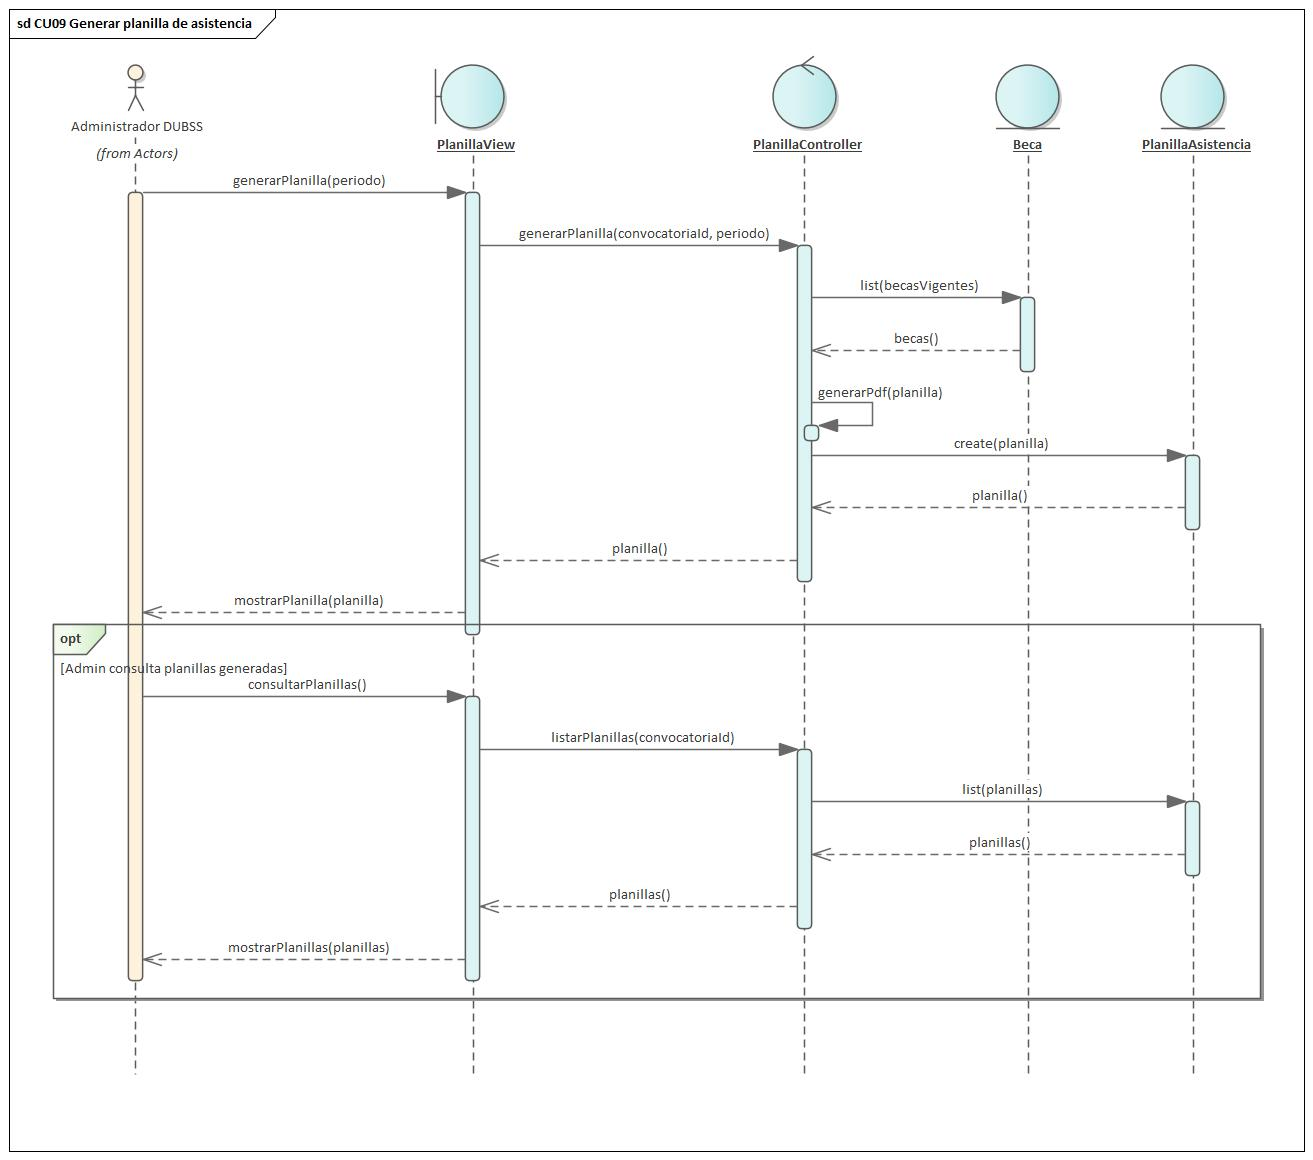
\includegraphics[width=\textwidth,height=0.75\textheight,keepaspectratio]{images/096_Secuencia_CU09_Generar_Planilla_Asistencia.jpg}

\smallskip
\noindent\raggedright\textit{Nota.} Elaboración propia.
\end{figure}


\Needspace{0.9\textheight}
\subsubsection{7.4.10. Diseñar CU-10 Registrar asistencia digital}\label{sec:cap7_disenar_cu10}

La Figura~\ref{fig:secuencia_cu10} presenta el diagrama de secuencia del CU-10.

\begin{figure}[H]
\caption{Diagrama de secuencia del CU-10 Registrar asistencia digital}
\label{fig:secuencia_cu10}
\centering
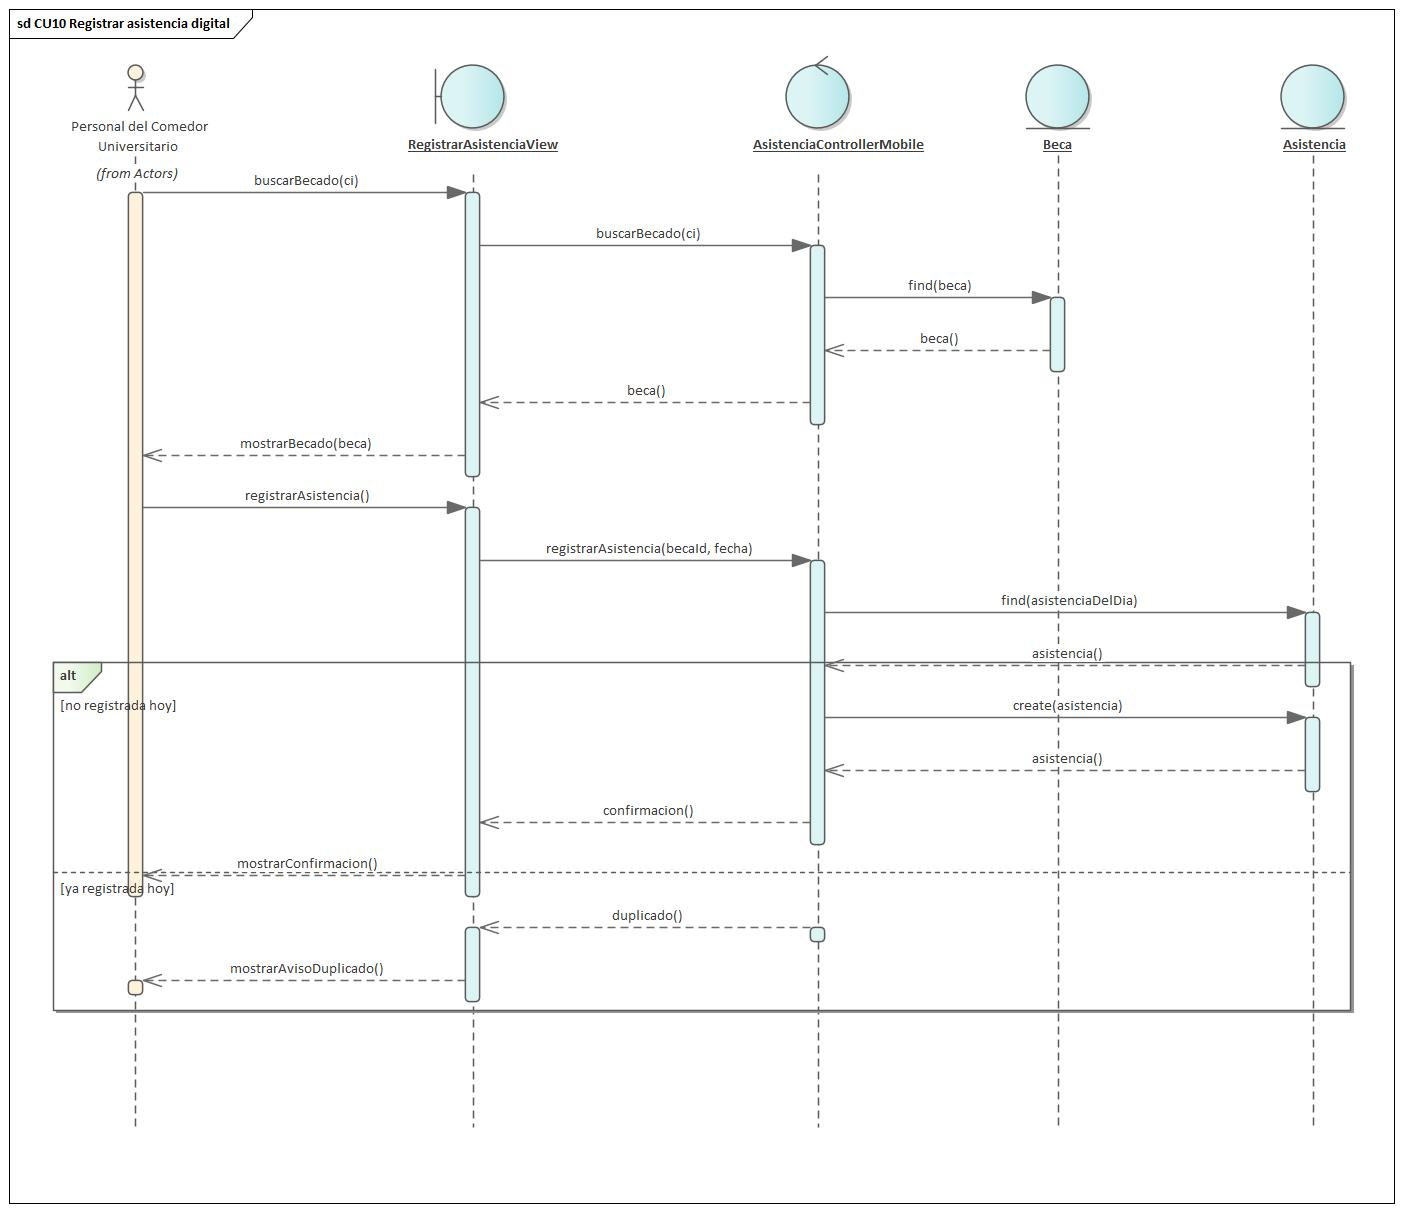
\includegraphics[width=\textwidth,height=0.75\textheight,keepaspectratio]{images/097_Secuencia_CU10_Registrar_Asistencia_Digital.jpg}

\smallskip
\noindent\raggedright\textit{Nota.} Elaboración propia.
\end{figure}


\Needspace{0.9\textheight}
\subsubsection{7.4.11. Diseñar CU-11 Cotejar registro contra respaldo físico}\label{sec:cap7_disenar_cu11}

La Figura~\ref{fig:secuencia_cu11} presenta el diagrama de secuencia del CU-11.

\begin{figure}[H]
\caption{Diagrama de secuencia del CU-11 Cotejar registro contra respaldo físico}
\label{fig:secuencia_cu11}
\centering
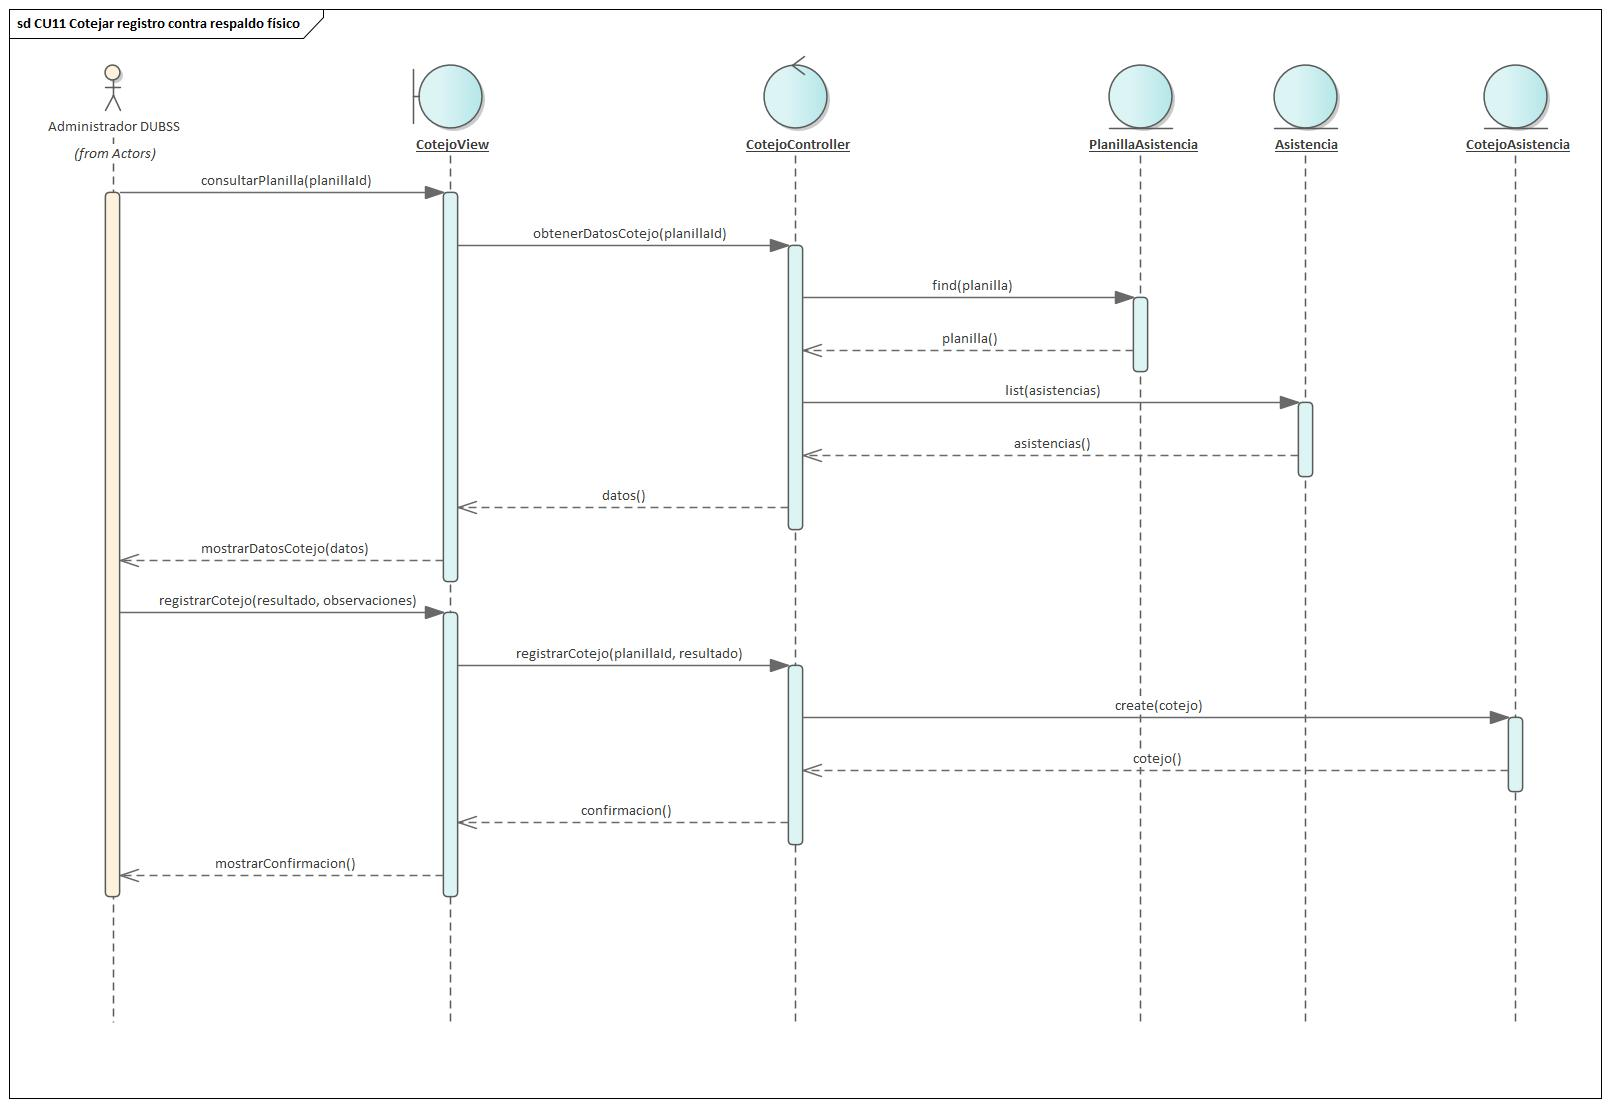
\includegraphics[width=\textwidth,height=0.75\textheight,keepaspectratio]{images/098_Secuencia_CU11_Cotejar_Registro_Respaldo_Fisico.jpg}

\smallskip
\noindent\raggedright\textit{Nota.} Elaboración propia.
\end{figure}


\Needspace{0.9\textheight}
\subsubsection{7.4.12. Diseñar CU-12 Visualizar dashboard de indicadores BI}\label{sec:cap7_disenar_cu12}

La Figura~\ref{fig:secuencia_cu12} presenta el diagrama de secuencia del CU-12.

\begin{figure}[H]
\caption{Diagrama de secuencia del CU-12 Visualizar dashboard de indicadores BI}
\label{fig:secuencia_cu12}
\centering
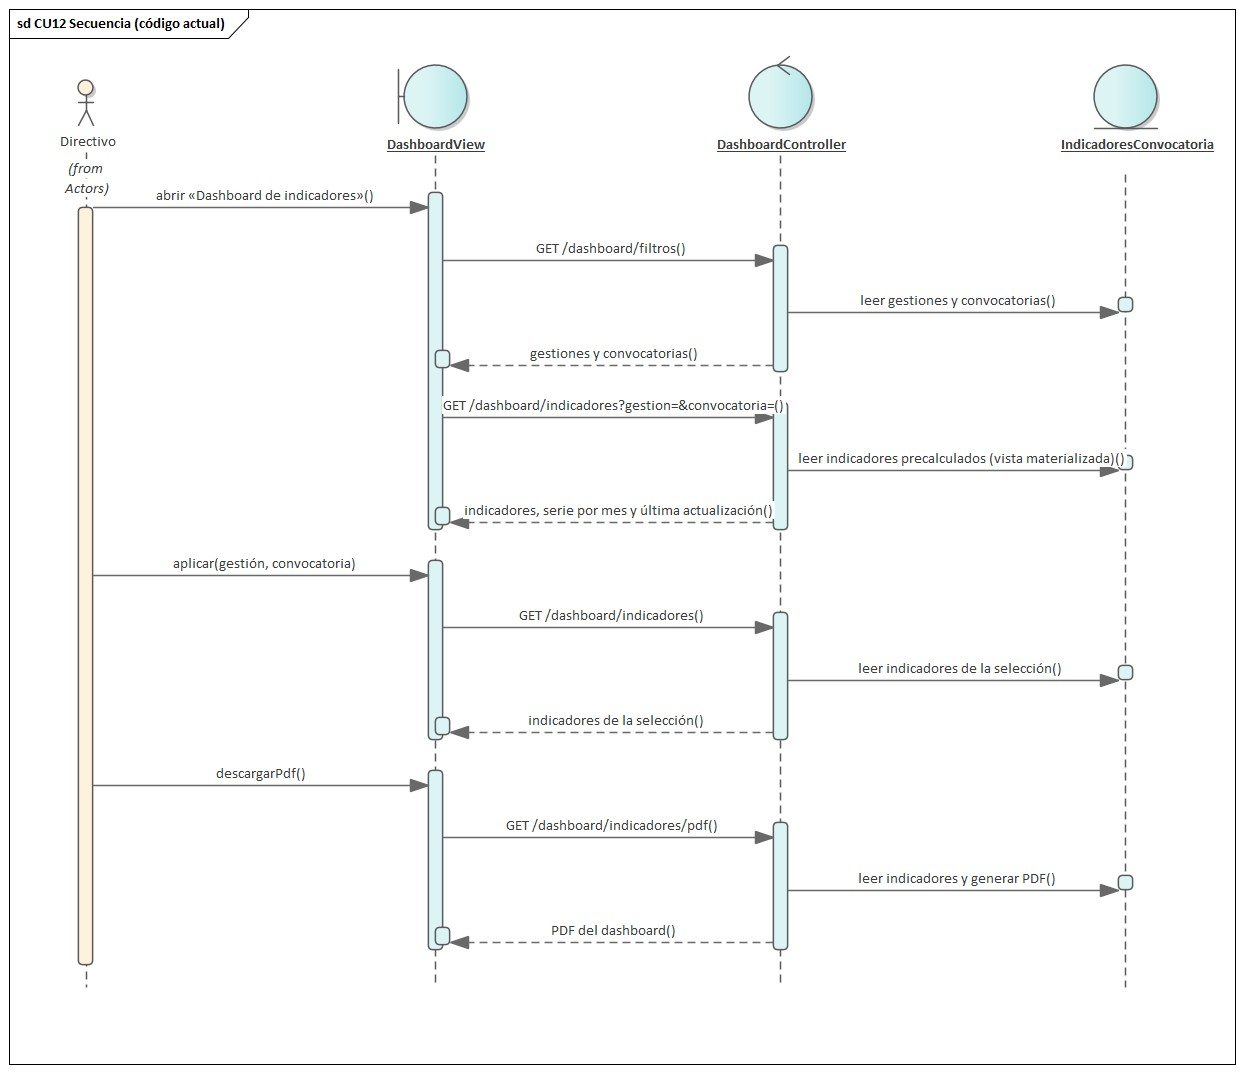
\includegraphics[width=\textwidth,height=0.75\textheight,keepaspectratio]{images/099_Secuencia_CU12_Visualizar_Dashboard_Indicadores_BI.jpg}

\smallskip
\noindent\raggedright\textit{Nota.} Elaboración propia.
\end{figure}


\Needspace{0.9\textheight}
\subsubsection{7.4.13. Diseñar CU-13 Gestionar convocatoria y gestión académica}\label{sec:cap7_disenar_cu13}

La Figura~\ref{fig:secuencia_cu13} presenta el diagrama de secuencia del CU-13.

\begin{figure}[H]
\caption{Diagrama de secuencia del CU-13 Gestionar convocatoria y gestión académica}
\label{fig:secuencia_cu13}
\centering
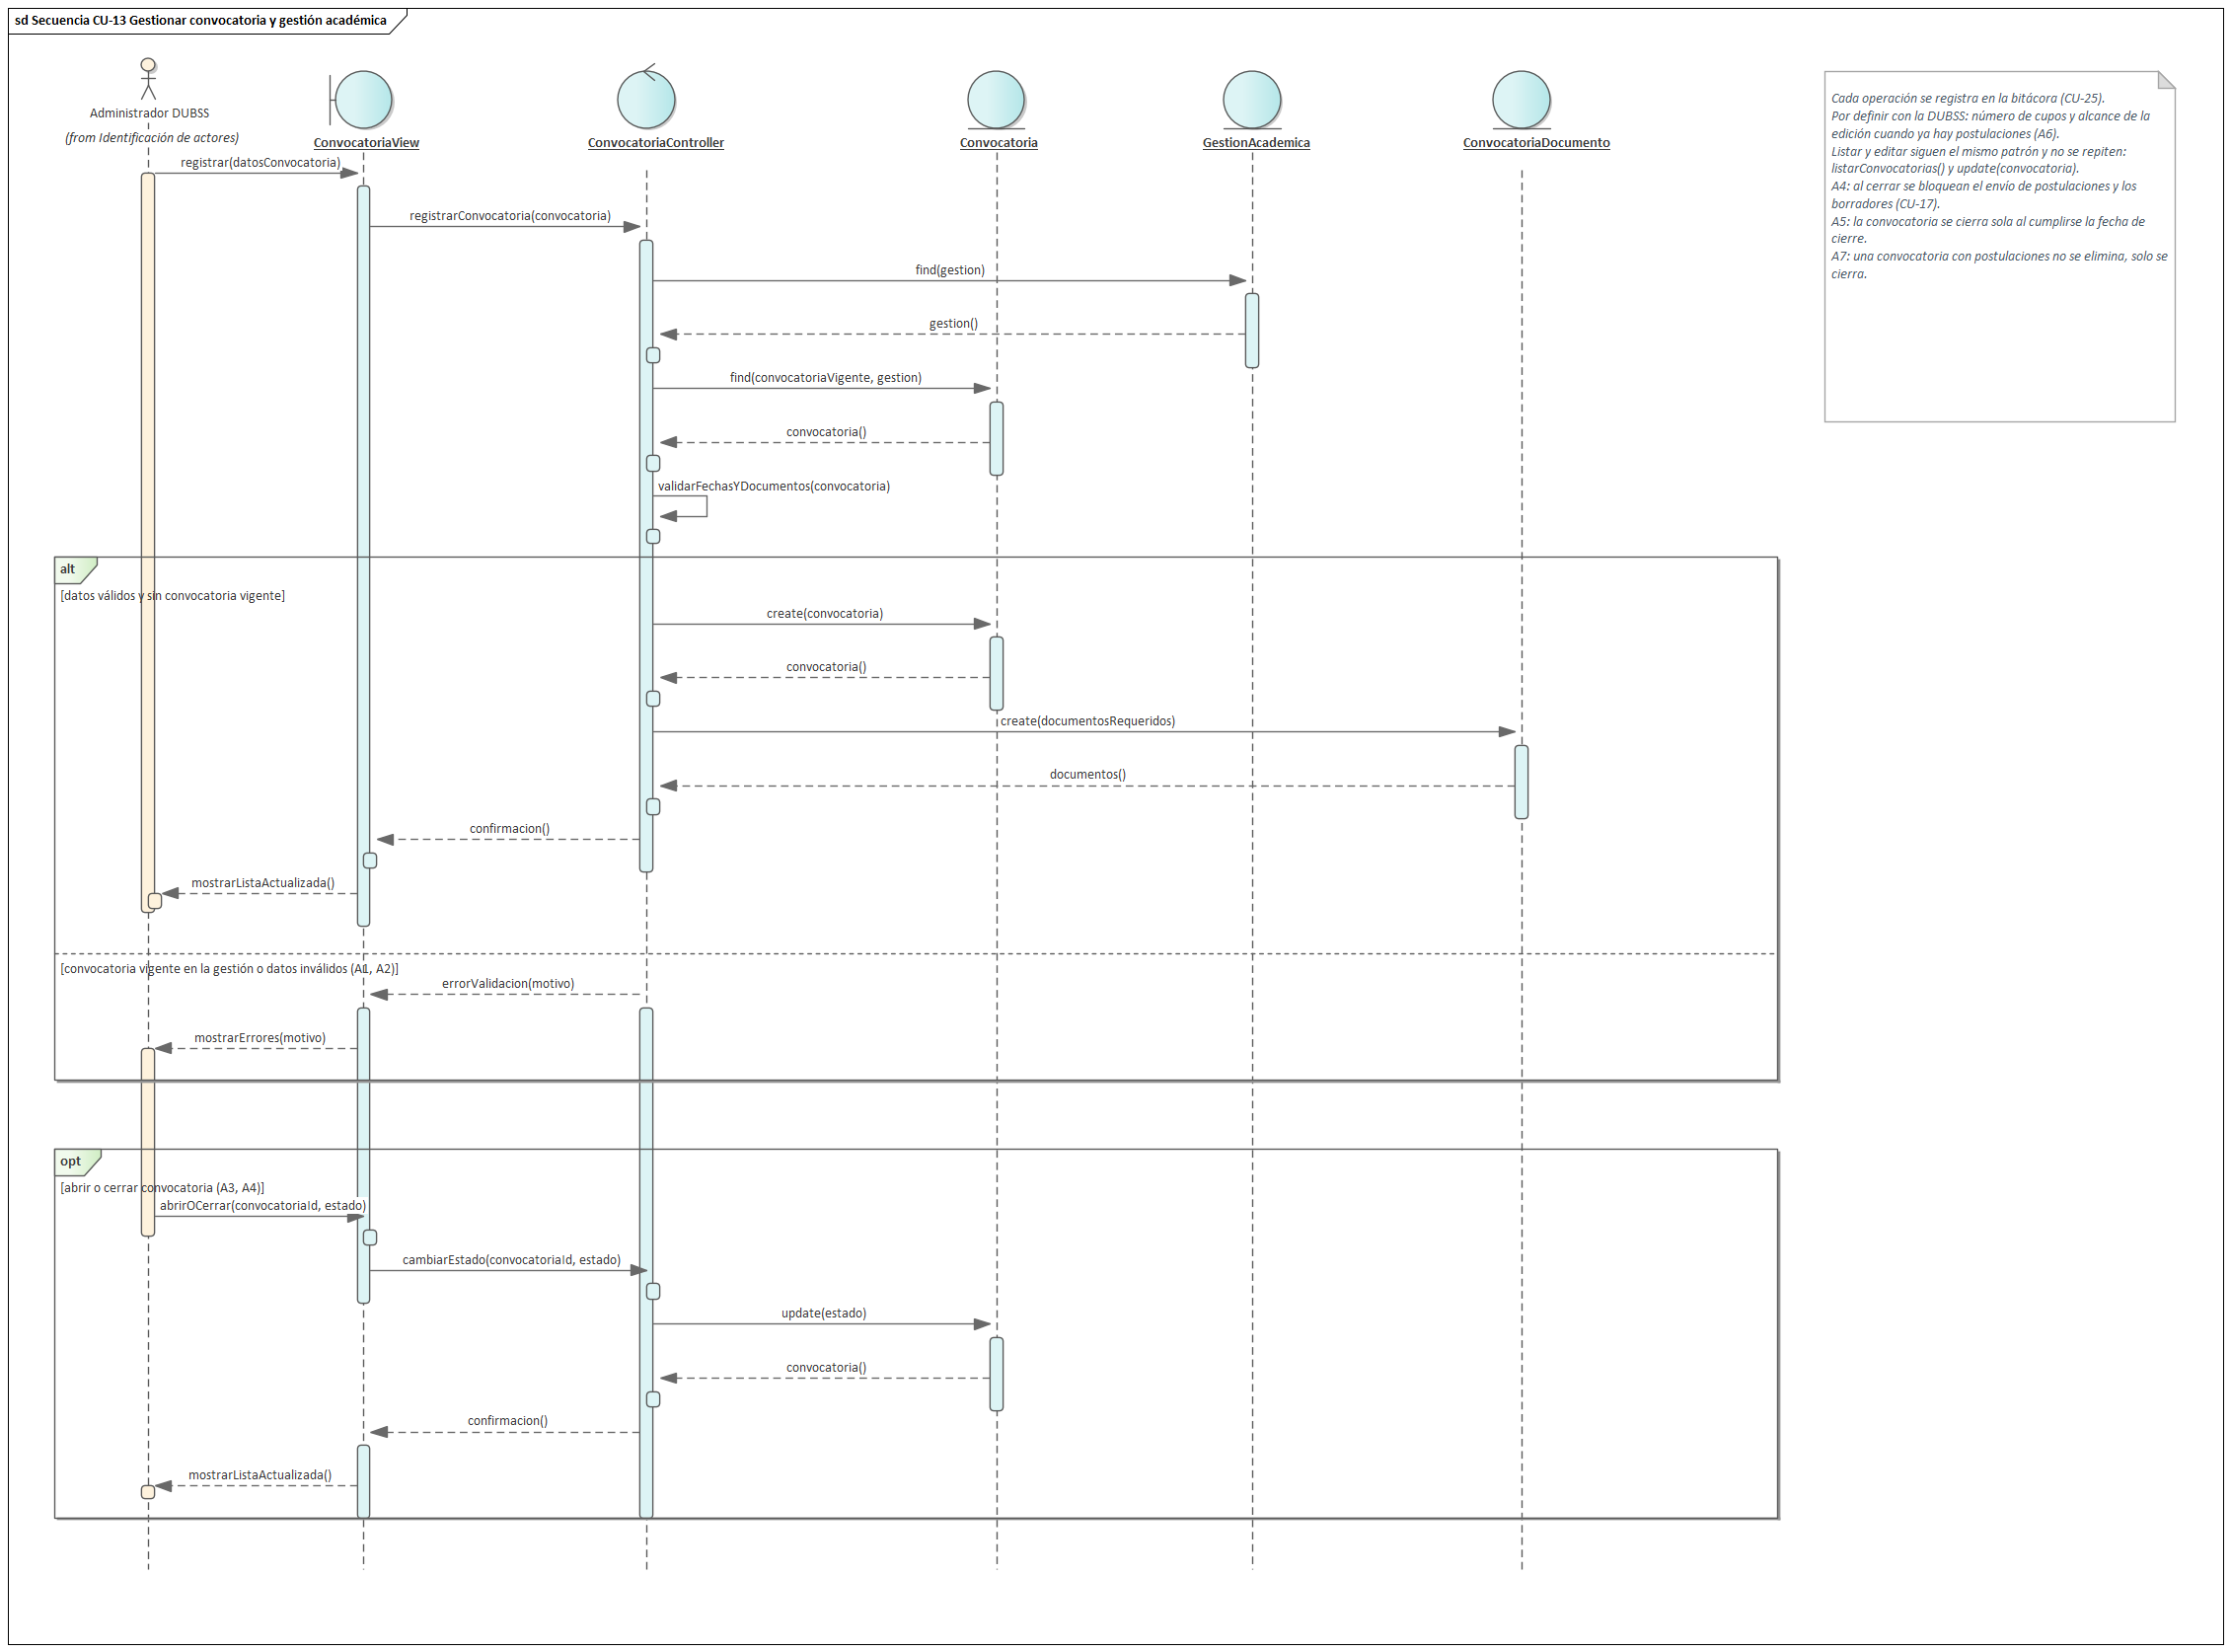
\includegraphics[width=\textwidth,height=0.75\textheight,keepaspectratio]{images/125_Secuencia_CU13_Gestionar_Convocatoria_Gestion_Academica.png}

\smallskip
\noindent\raggedright\textit{Nota.} Elaboración propia.
\end{figure}


\Needspace{0.9\textheight}
\subsubsection{7.4.14. Diseñar CU-14 Gestionar usuarios y roles}\label{sec:cap7_disenar_cu14}

La Figura~\ref{fig:secuencia_cu14} presenta el diagrama de secuencia del CU-14.

\begin{figure}[H]
\caption{Diagrama de secuencia del CU-14 Gestionar usuarios y roles}
\label{fig:secuencia_cu14}
\centering
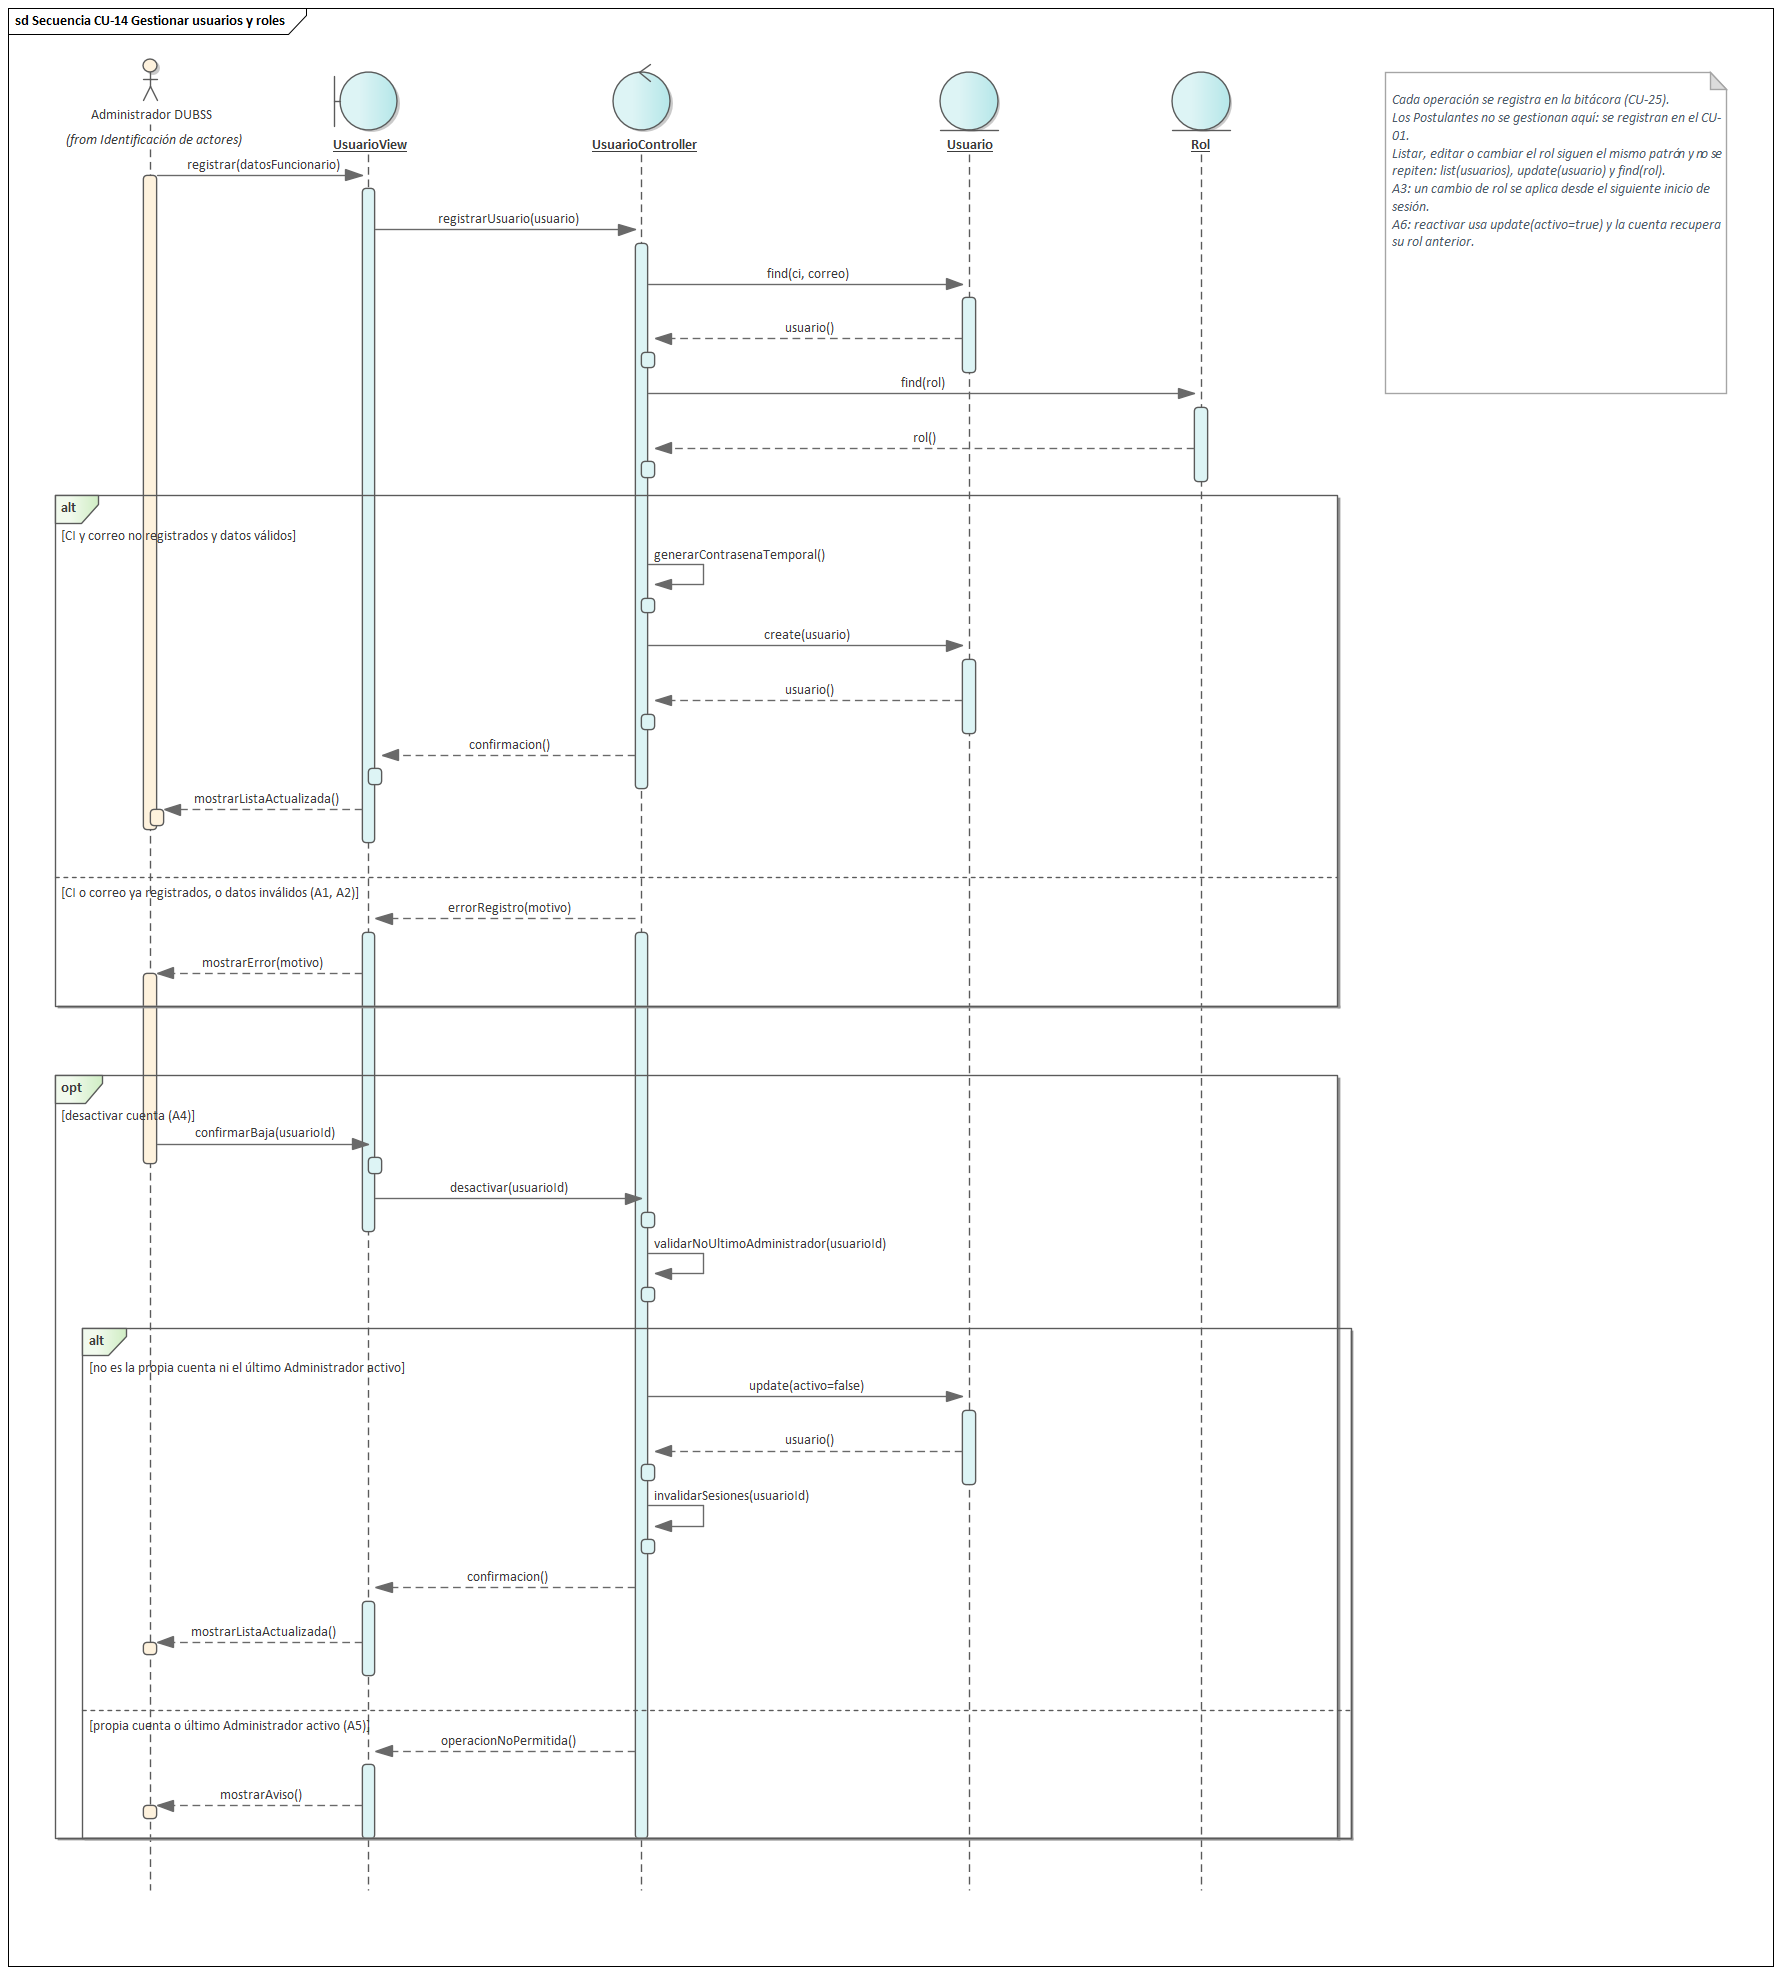
\includegraphics[width=\textwidth,height=0.75\textheight,keepaspectratio]{images/126_Secuencia_CU14_Gestionar_Usuarios_Roles.png}

\smallskip
\noindent\raggedright\textit{Nota.} Elaboración propia.
\end{figure}


\Needspace{0.9\textheight}
\subsubsection{7.4.15. Diseñar CU-15 Recuperar contraseña / gestionar perfil}\label{sec:cap7_disenar_cu15}

La Figura~\ref{fig:secuencia_cu15} presenta el diagrama de secuencia del CU-15.

\begin{figure}[H]
\caption{Diagrama de secuencia del CU-15 Recuperar contraseña / gestionar perfil}
\label{fig:secuencia_cu15}
\centering
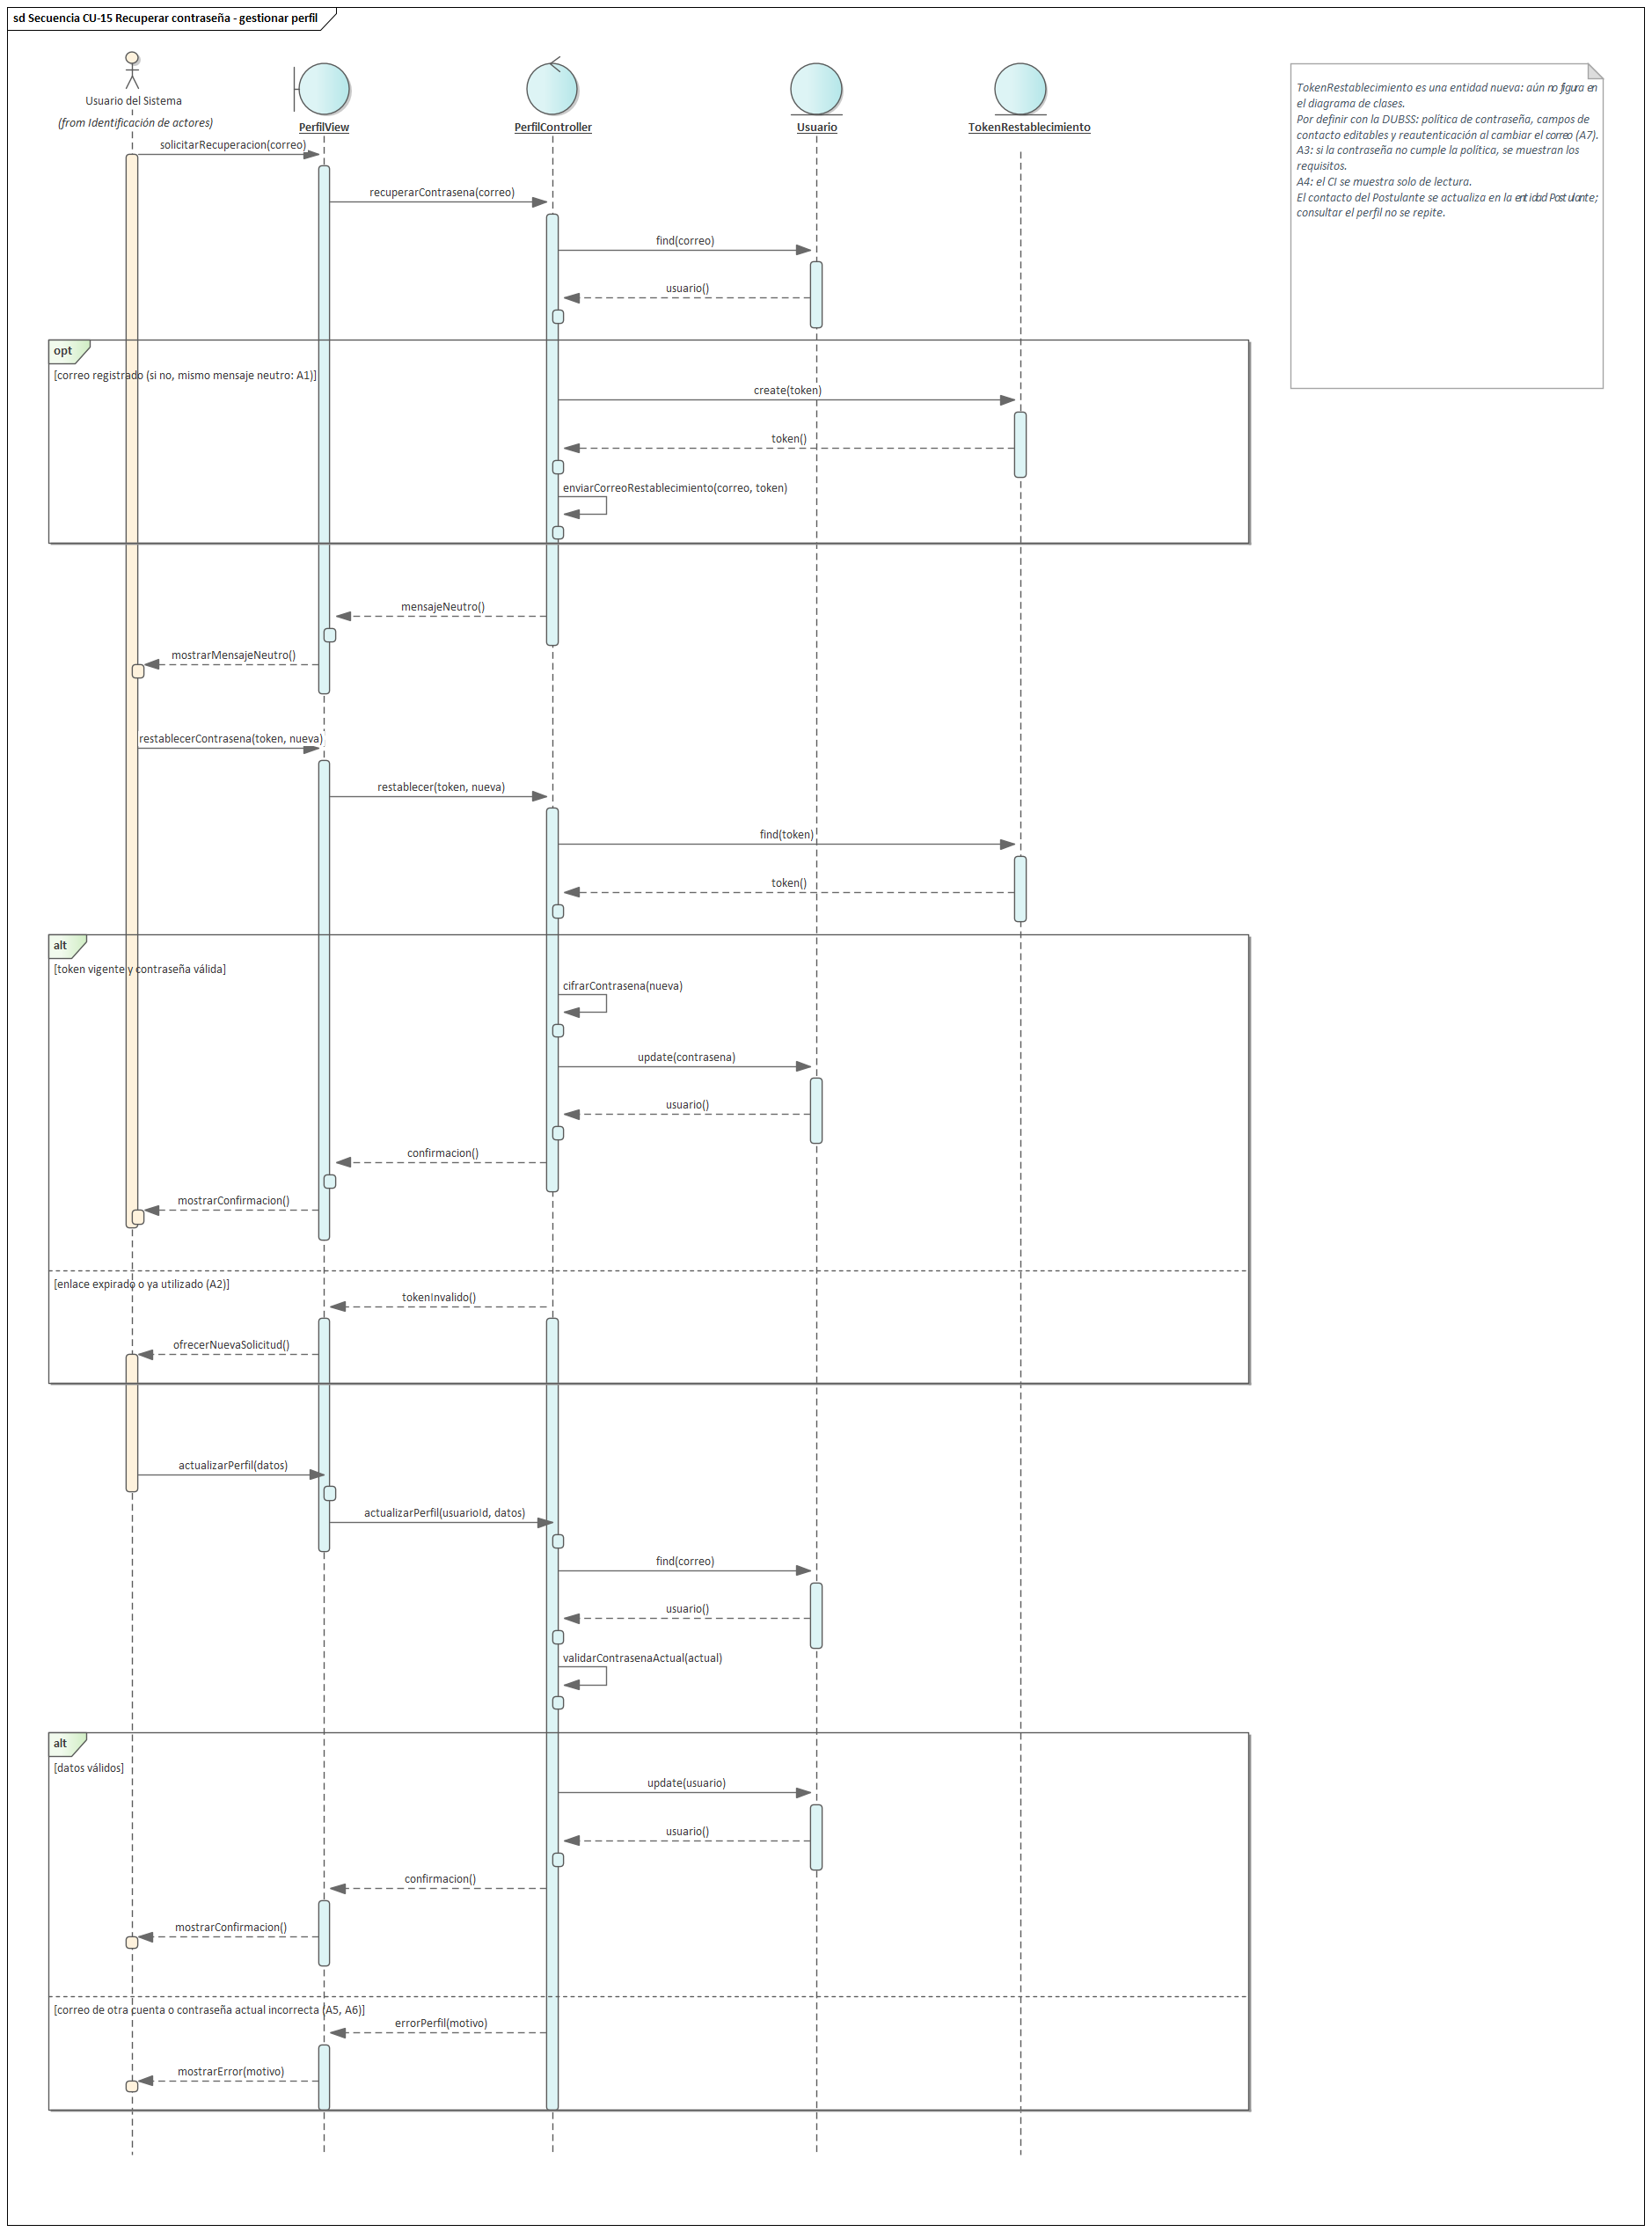
\includegraphics[width=\textwidth,height=0.75\textheight,keepaspectratio]{images/127_Secuencia_CU15_Recuperar_Contrasena_Gestionar_Perfil.png}

\smallskip
\noindent\raggedright\textit{Nota.} Elaboración propia.
\end{figure}


\Needspace{0.9\textheight}
\subsubsection{7.4.16. Diseñar CU-16 Digitalizar y adjuntar documentos}\label{sec:cap7_disenar_cu16}

La Figura~\ref{fig:secuencia_cu16} presenta el diagrama de secuencia del CU-16.

\begin{figure}[H]
\caption{Diagrama de secuencia del CU-16 Digitalizar y adjuntar documentos}
\label{fig:secuencia_cu16}
\centering
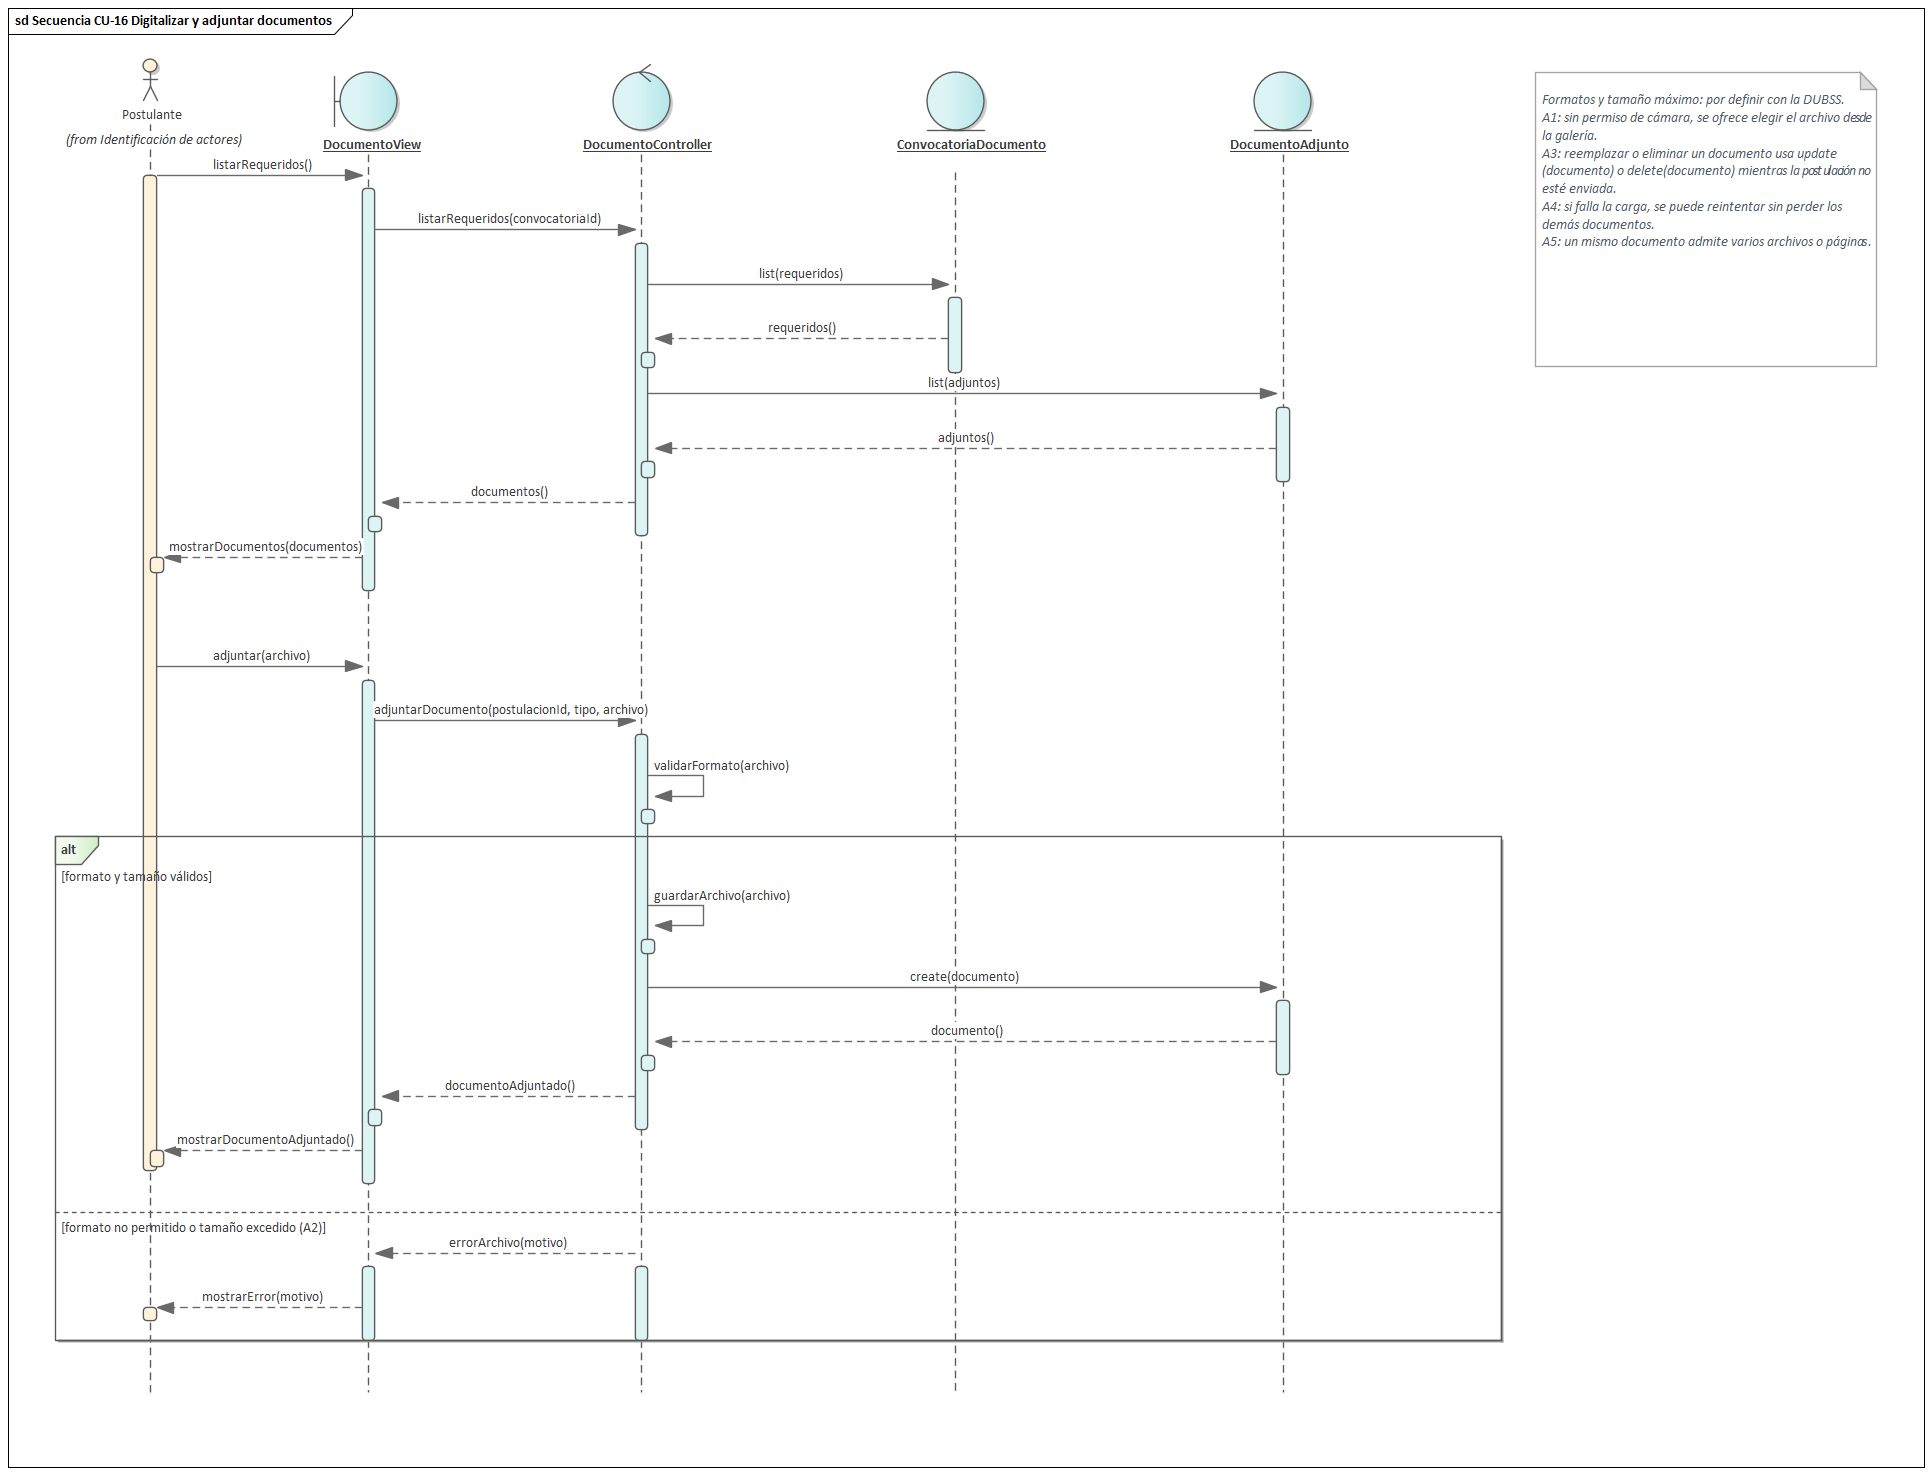
\includegraphics[width=\textwidth,height=0.75\textheight,keepaspectratio]{images/128_Secuencia_CU16_Digitalizar_Adjuntar_Documentos.png}

\smallskip
\noindent\raggedright\textit{Nota.} Elaboración propia.
\end{figure}


\Needspace{0.9\textheight}
\subsubsection{7.4.17. Diseñar CU-17 Guardar borrador de postulación}\label{sec:cap7_disenar_cu17}

La Figura~\ref{fig:secuencia_cu17} presenta el diagrama de secuencia del CU-17.

\begin{figure}[H]
\caption{Diagrama de secuencia del CU-17 Guardar borrador de postulación}
\label{fig:secuencia_cu17}
\centering
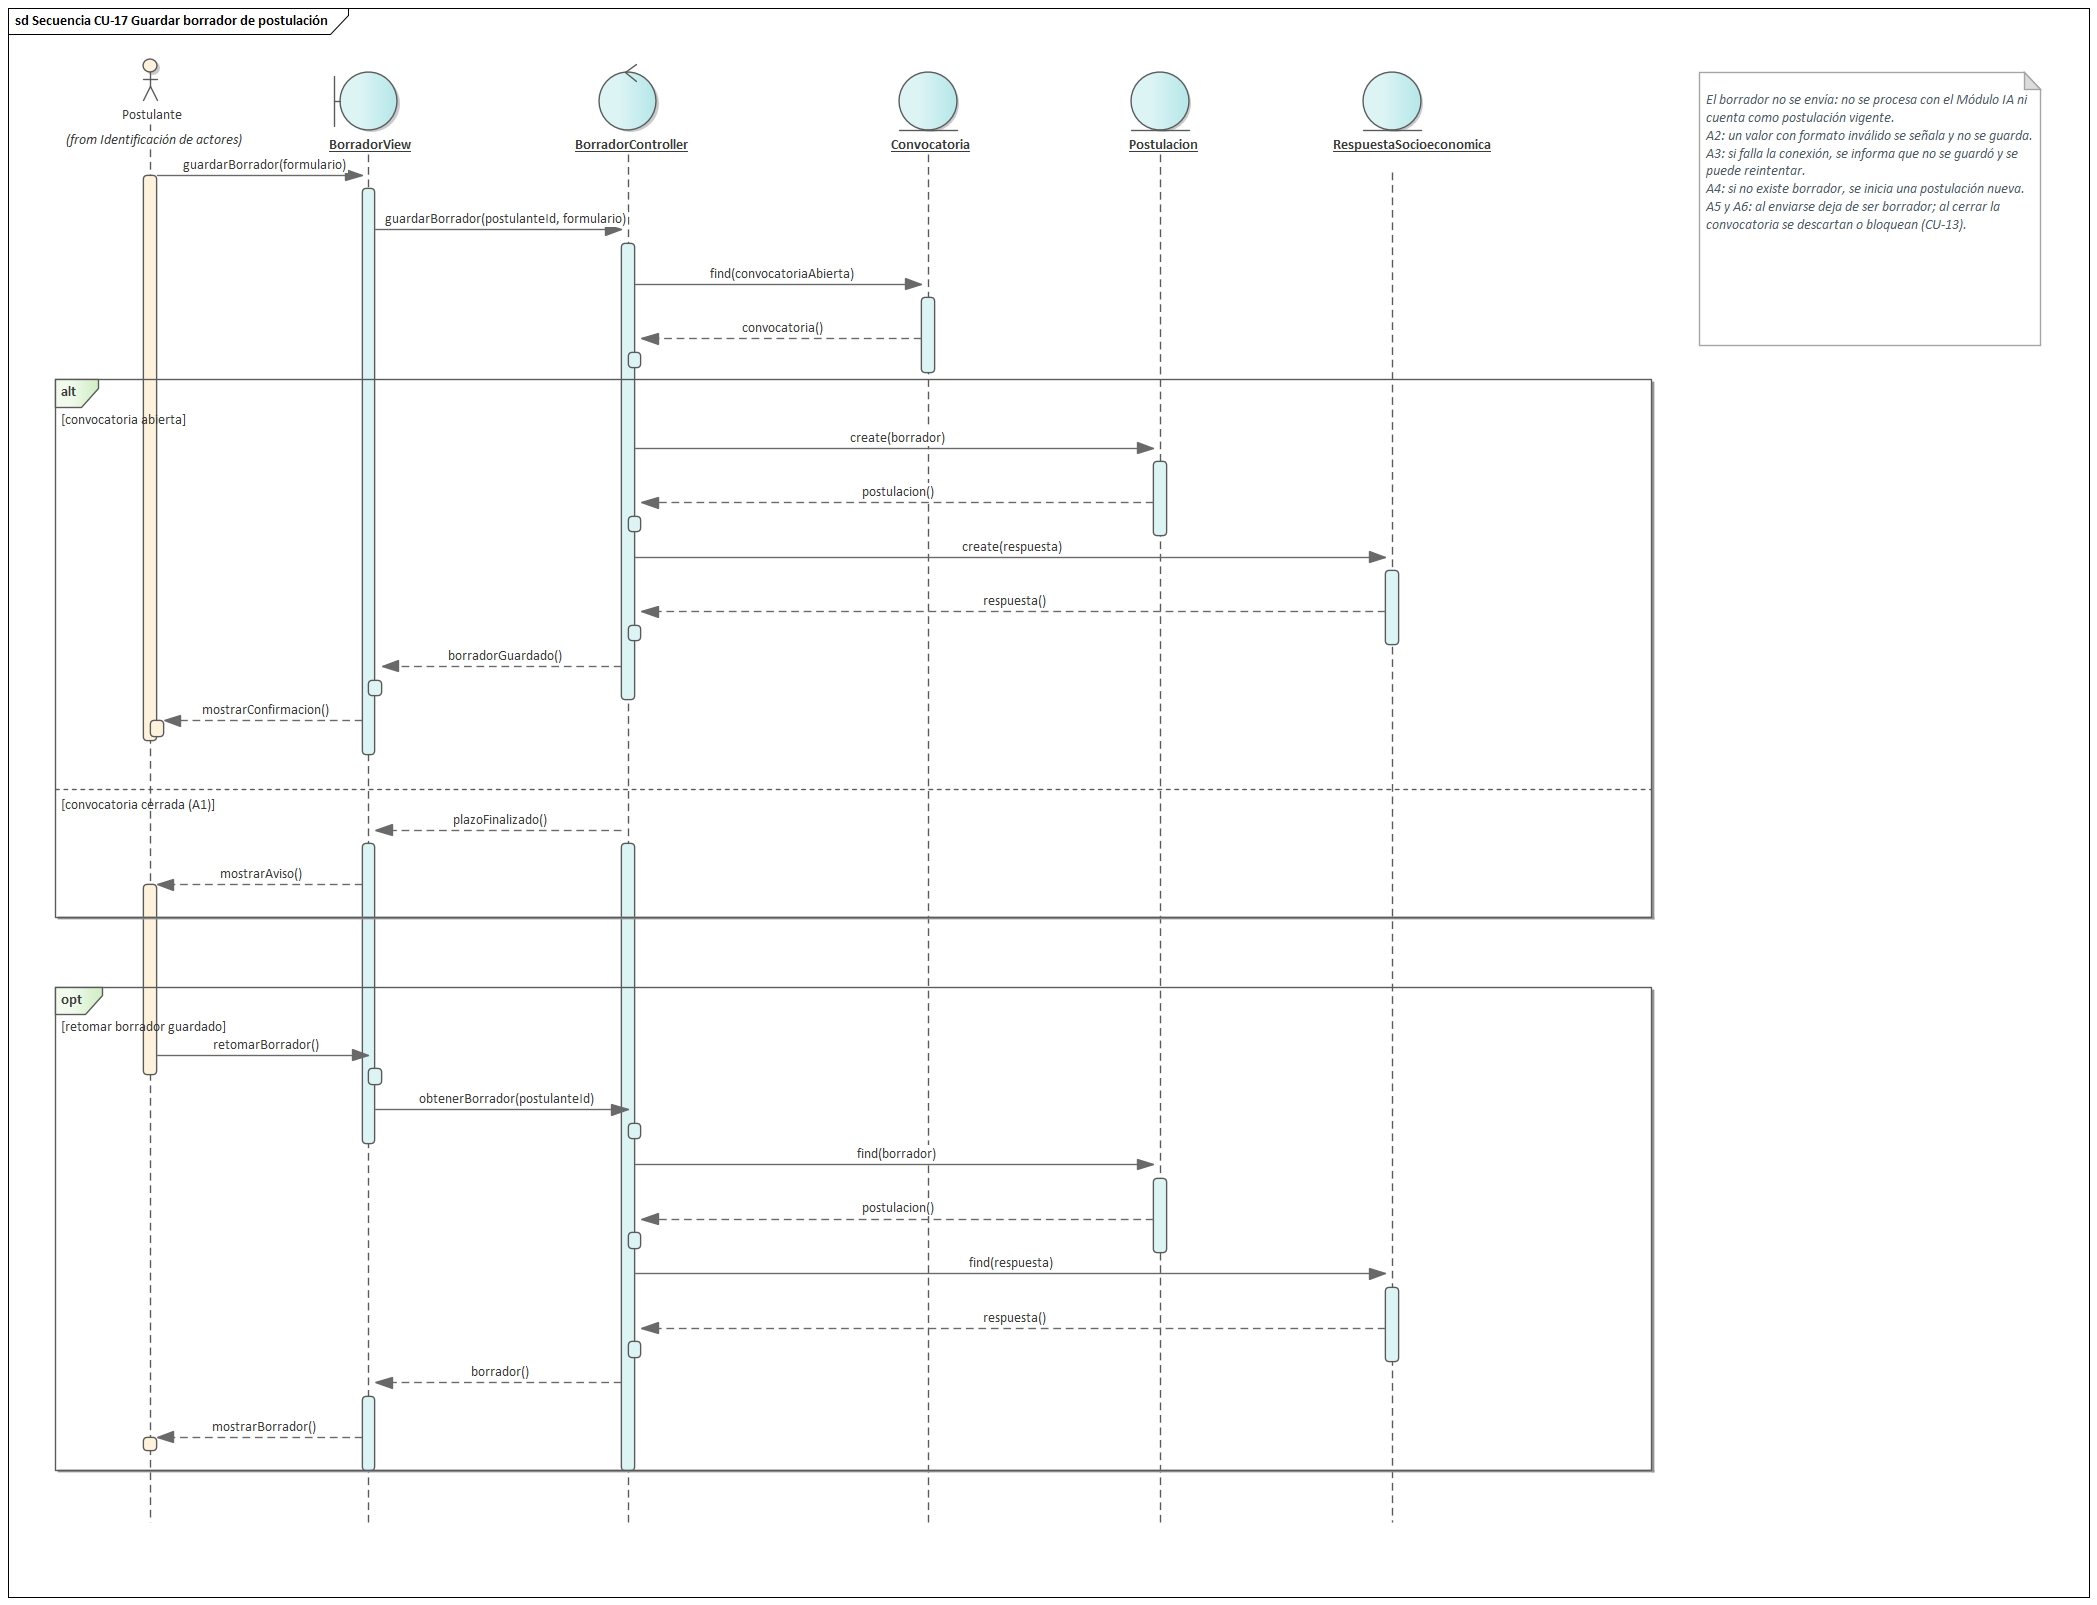
\includegraphics[width=\textwidth,height=0.75\textheight,keepaspectratio]{images/129_Secuencia_CU17_Guardar_Borrador_Postulacion.png}

\smallskip
\noindent\raggedright\textit{Nota.} Elaboración propia.
\end{figure}


\Needspace{0.9\textheight}
\subsubsection{7.4.18. Diseñar CU-18 Validar elegibilidad y duplicados}\label{sec:cap7_disenar_cu18}

La Figura~\ref{fig:secuencia_cu18} presenta el diagrama de secuencia del CU-18.

\begin{figure}[H]
\caption{Diagrama de secuencia del CU-18 Validar elegibilidad y duplicados}
\label{fig:secuencia_cu18}
\centering
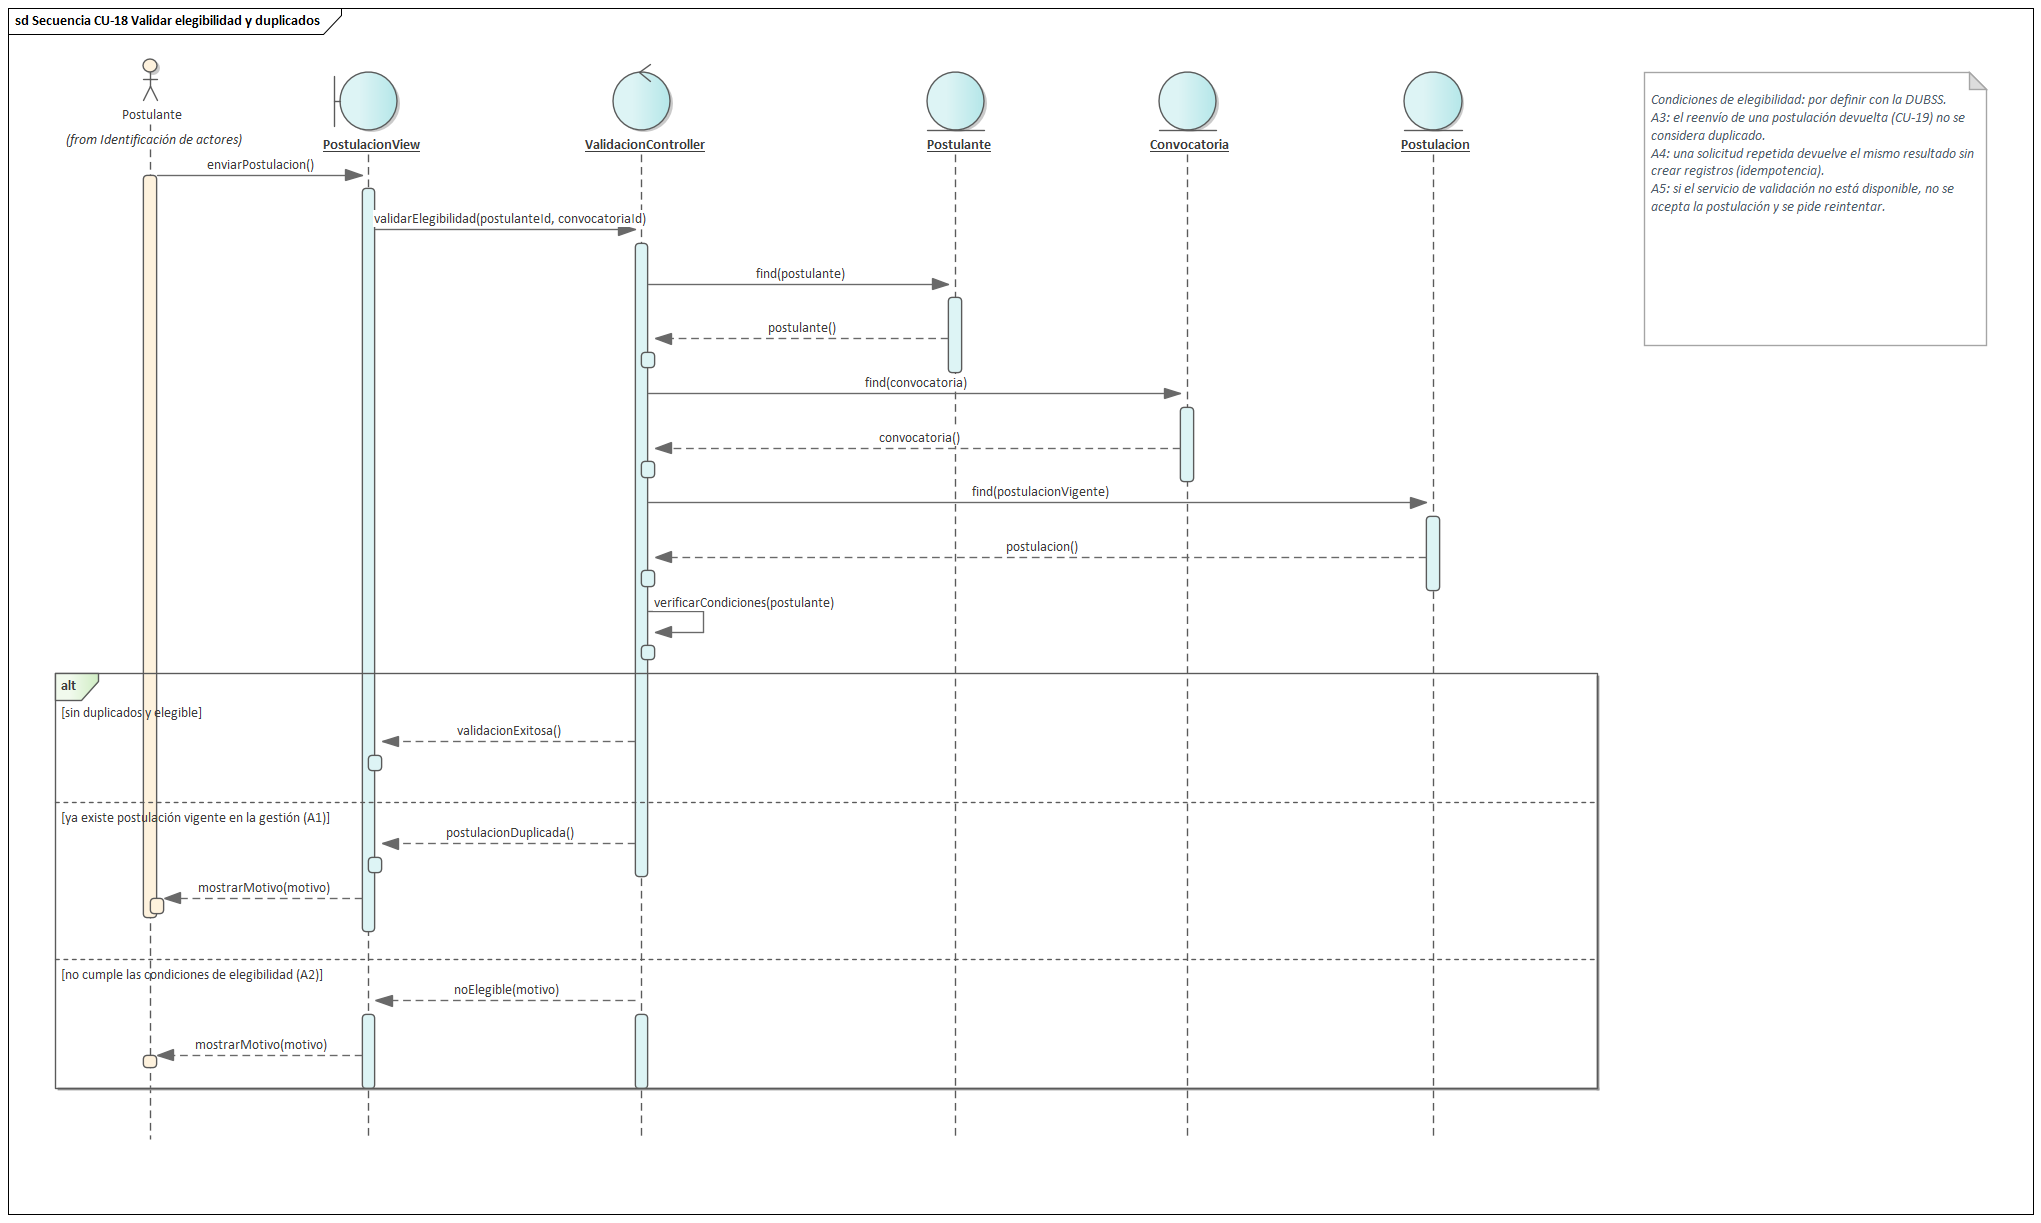
\includegraphics[width=\textwidth,height=0.75\textheight,keepaspectratio]{images/130_Secuencia_CU18_Validar_Elegibilidad_Duplicados.png}

\smallskip
\noindent\raggedright\textit{Nota.} Elaboración propia.
\end{figure}


\Needspace{0.9\textheight}
\subsubsection{7.4.19. Diseñar CU-19 Devolver postulación para corrección}\label{sec:cap7_disenar_cu19}

La Figura~\ref{fig:secuencia_cu19} presenta el diagrama de secuencia del CU-19.

\begin{figure}[H]
\caption{Diagrama de secuencia del CU-19 Devolver postulación para corrección}
\label{fig:secuencia_cu19}
\centering
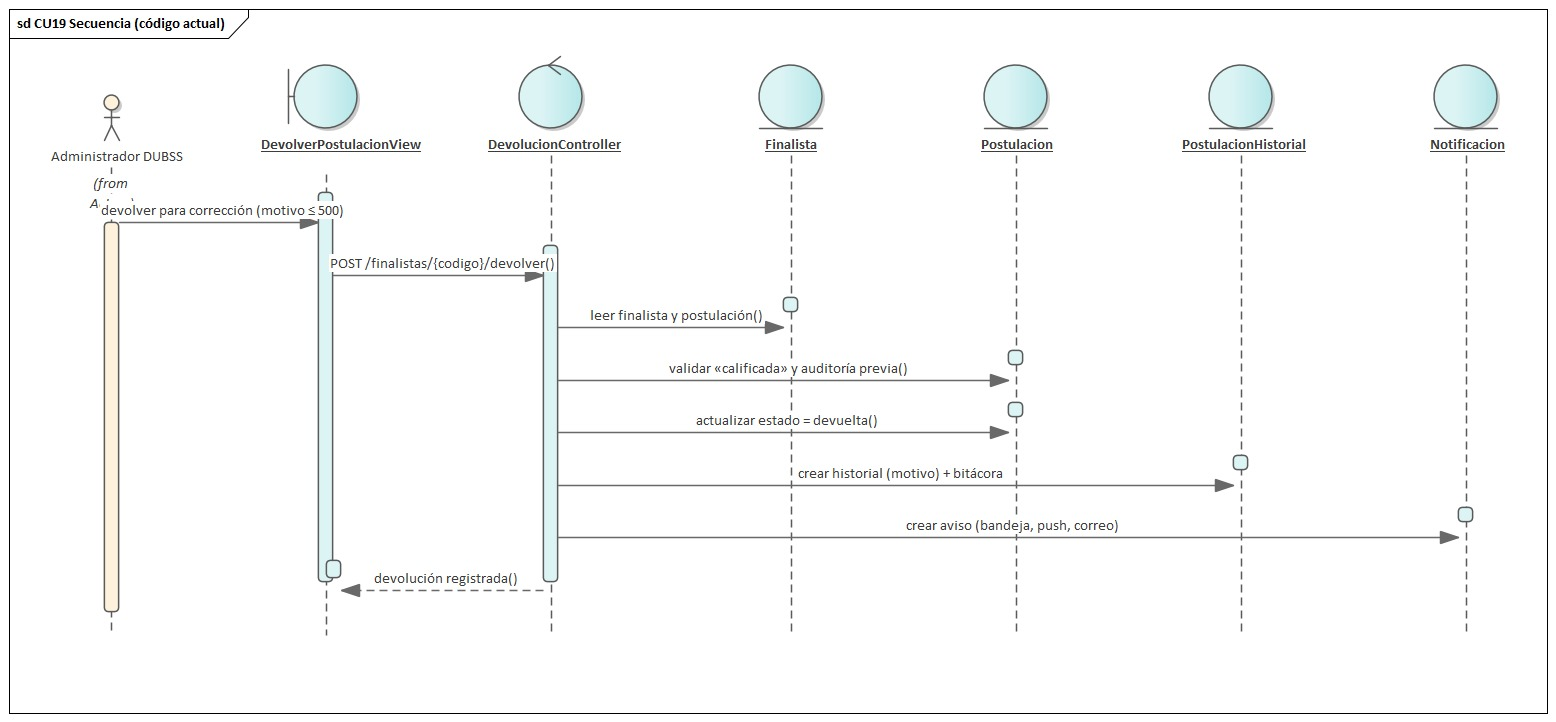
\includegraphics[width=\textwidth,height=0.75\textheight,keepaspectratio]{images/100_Secuencia_CU19_Devolver_Postulacion_Correccion.jpg}

\smallskip
\noindent\raggedright\textit{Nota.} Elaboración propia.
\end{figure}


\Needspace{0.9\textheight}
\subsubsection{7.4.20. Diseñar CU-20 Archivar o rechazar postulación}\label{sec:cap7_disenar_cu20}

La Figura~\ref{fig:secuencia_cu20} presenta el diagrama de secuencia del CU-20.

\begin{figure}[H]
\caption{Diagrama de secuencia del CU-20 Archivar o rechazar postulación}
\label{fig:secuencia_cu20}
\centering
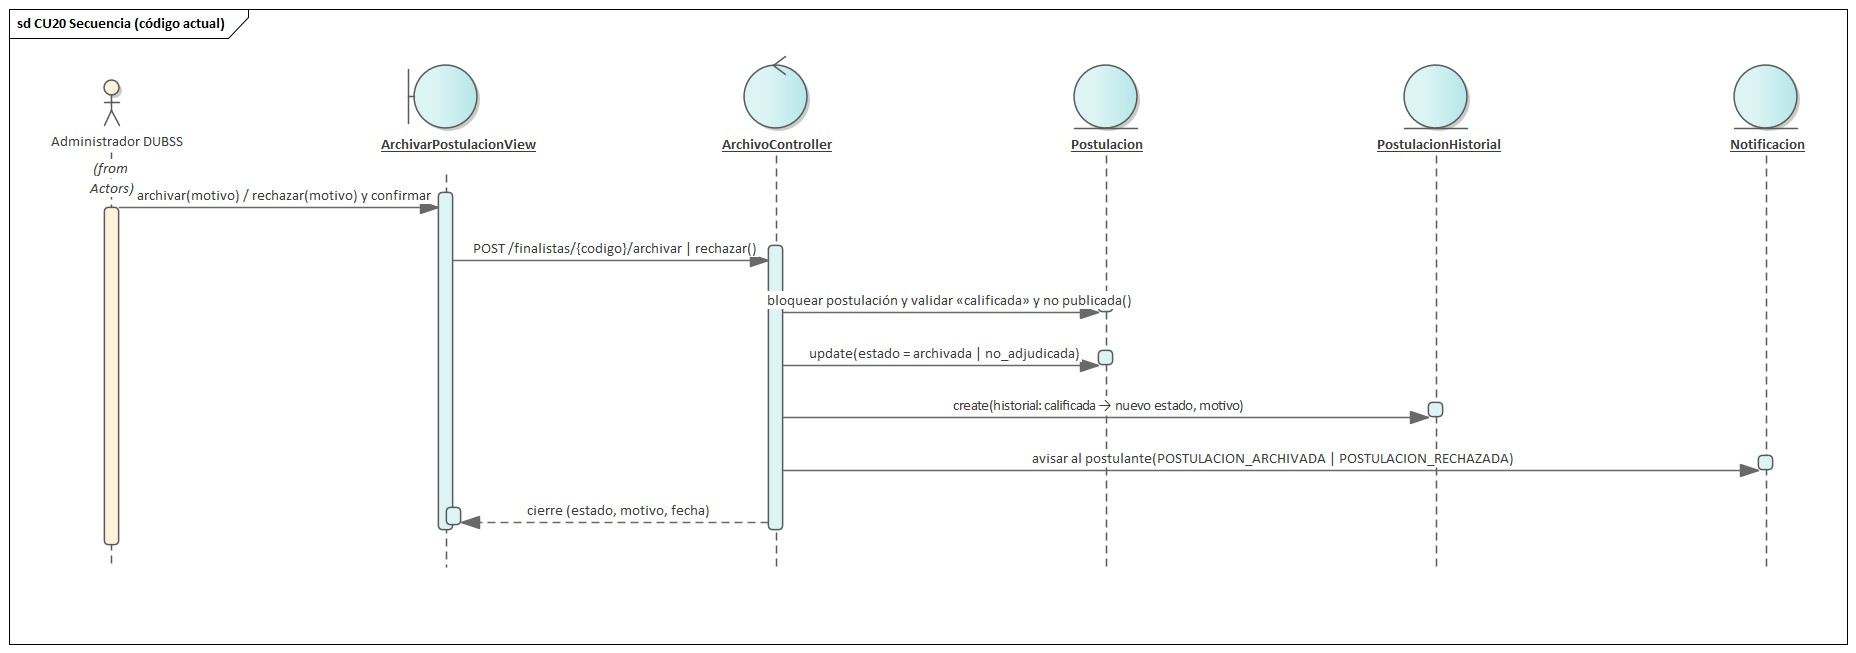
\includegraphics[width=\textwidth,height=0.75\textheight,keepaspectratio]{images/101_Secuencia_CU20_Archivar_Rechazar_Postulacion.jpg}

\smallskip
\noindent\raggedright\textit{Nota.} Elaboración propia.
\end{figure}


\Needspace{0.9\textheight}
\subsubsection{7.4.21. Diseñar CU-21 Notificar finalistas, registrar entrega de documentación física y publicar comunicados/avisos}\label{sec:cap7_disenar_cu21}

La Figura~\ref{fig:secuencia_cu21} presenta el diagrama de secuencia del CU-21.

\begin{figure}[H]
\caption{Diagrama de secuencia del CU-21 Notificar finalistas, registrar entrega de documentación física y publicar comunicados/avisos}
\label{fig:secuencia_cu21}
\centering
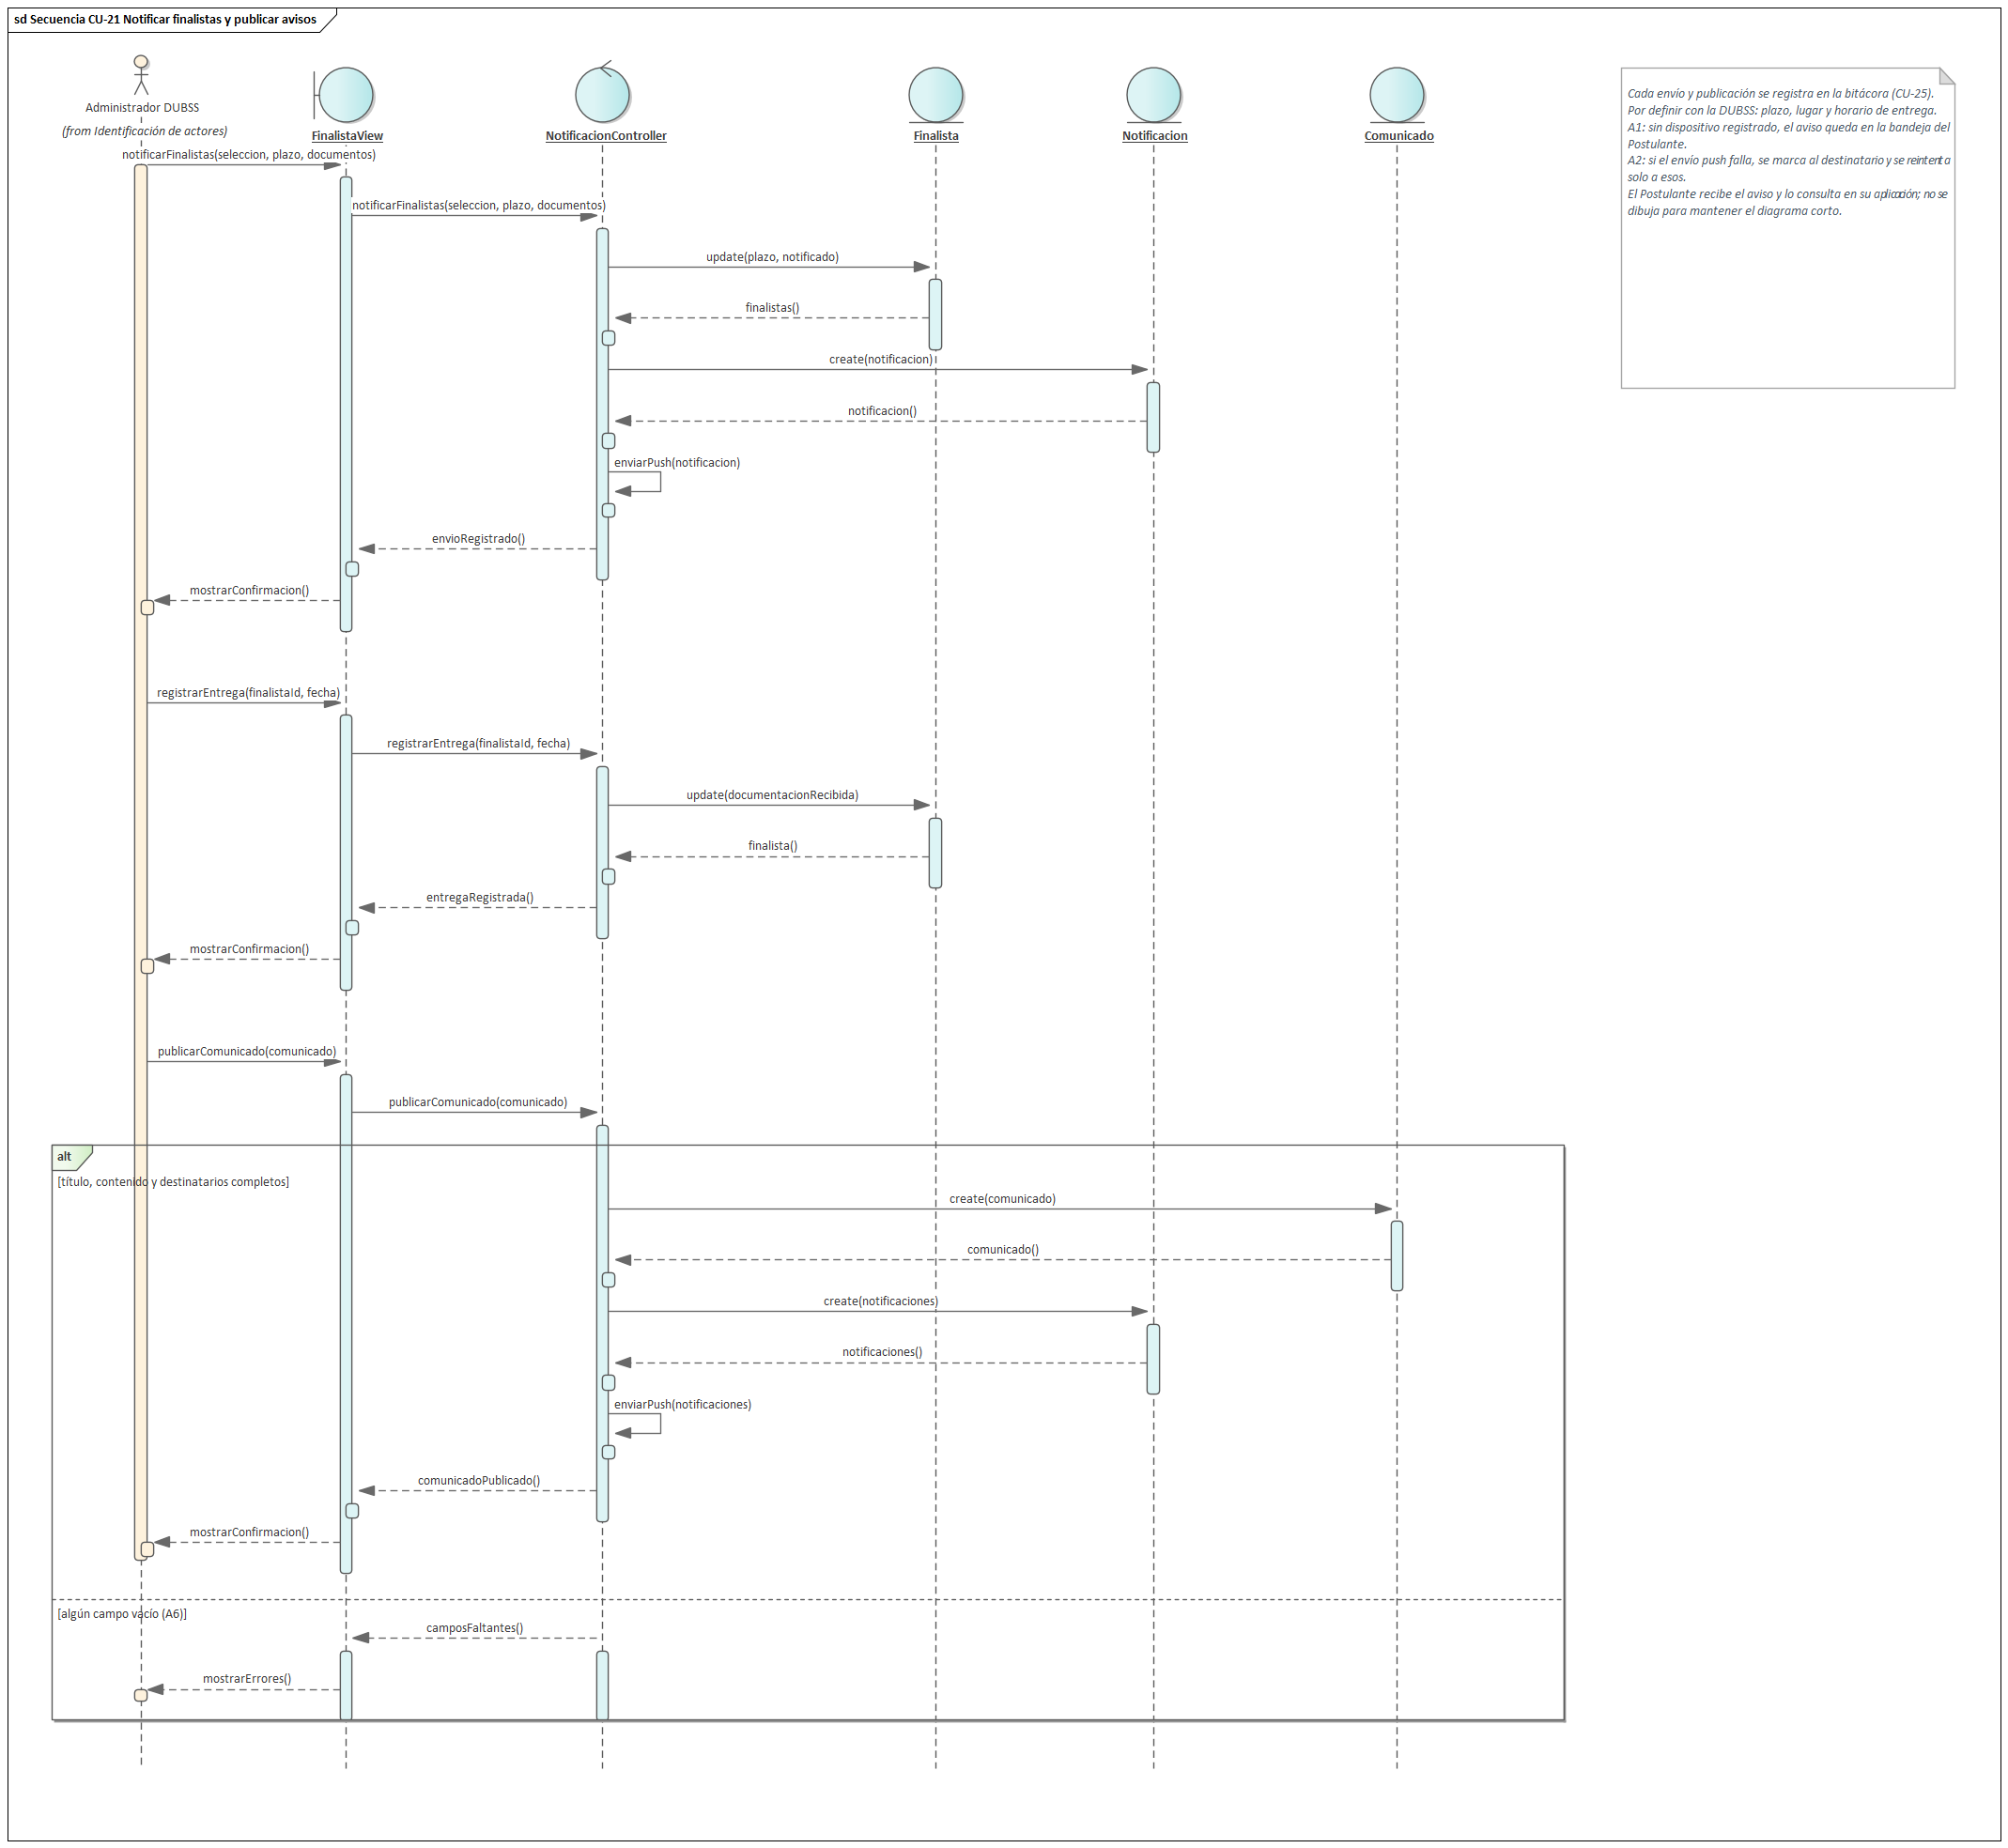
\includegraphics[width=\textwidth,height=0.75\textheight,keepaspectratio]{images/131_Secuencia_CU21_Notificar_Finalistas_Publicar_Avisos.png}

\smallskip
\noindent\raggedright\textit{Nota.} Elaboración propia.
\end{figure}


\Needspace{0.9\textheight}
\subsubsection{7.4.22. Diseñar CU-22 Publicar resultados de adjudicación}\label{sec:cap7_disenar_cu22}

La Figura~\ref{fig:secuencia_cu22} presenta el diagrama de secuencia del CU-22.

\begin{figure}[H]
\caption{Diagrama de secuencia del CU-22 Publicar resultados de adjudicación}
\label{fig:secuencia_cu22}
\centering
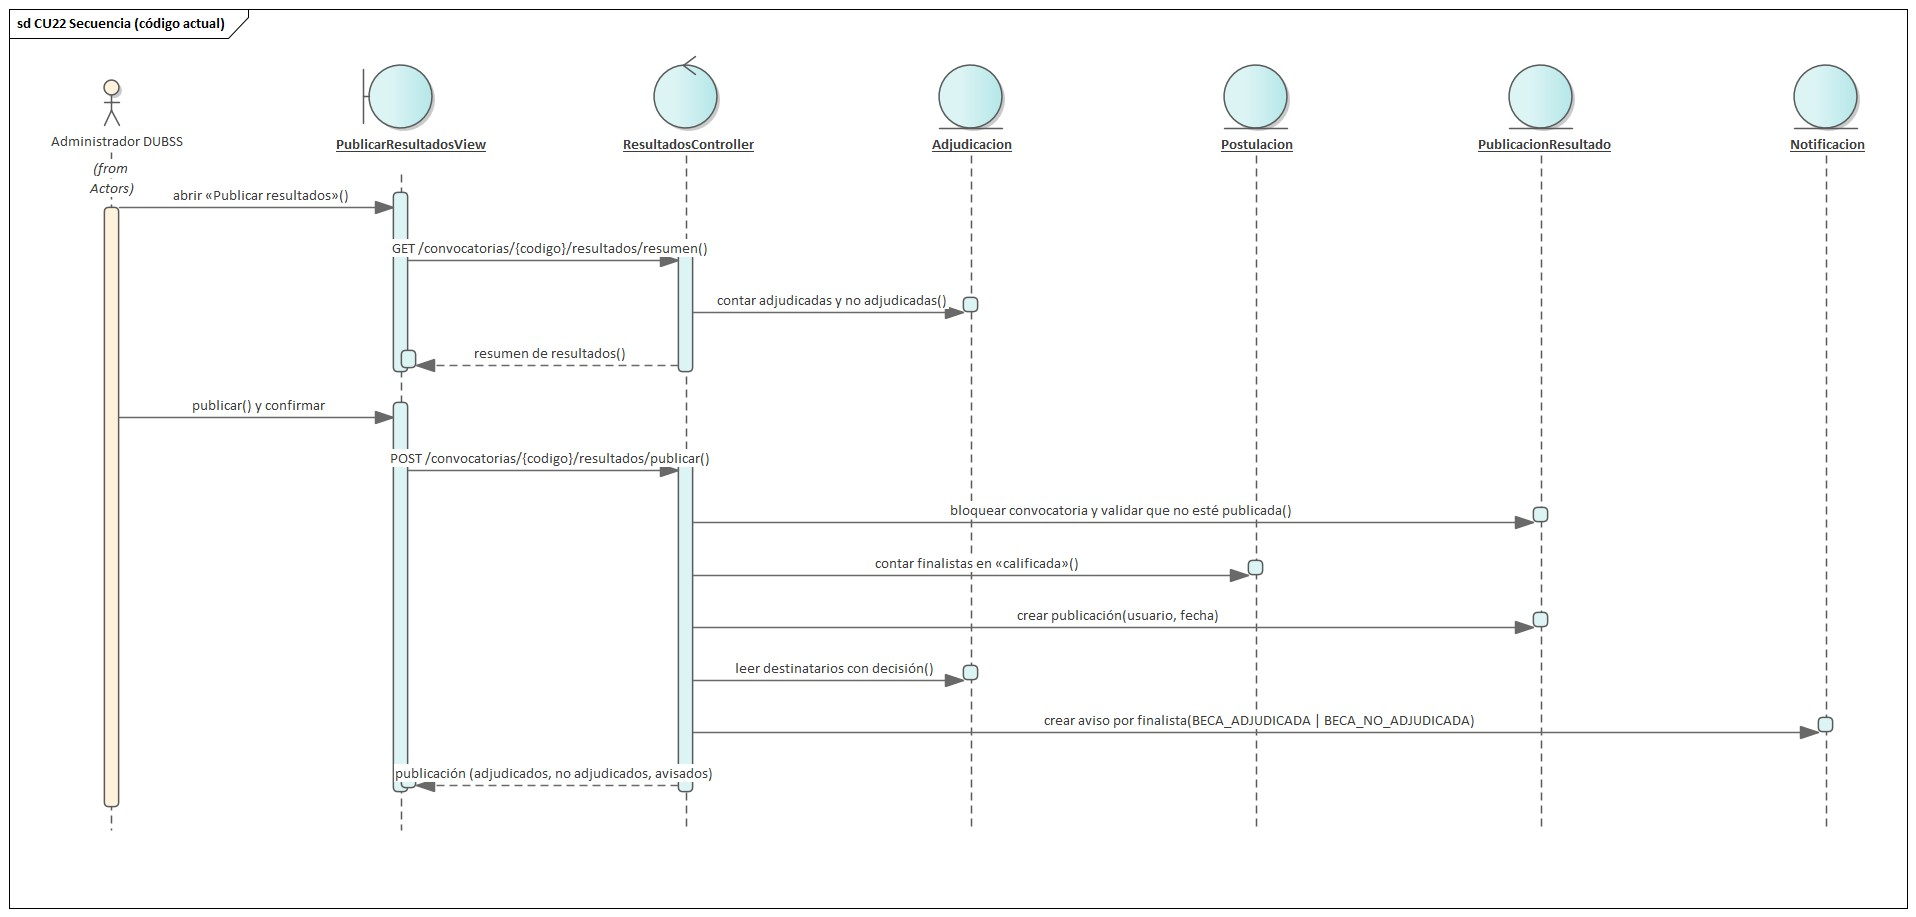
\includegraphics[width=\textwidth,height=0.75\textheight,keepaspectratio]{images/102_Secuencia_CU22_Publicar_Resultados_Adjudicacion.jpg}

\smallskip
\noindent\raggedright\textit{Nota.} Elaboración propia.
\end{figure}


\Needspace{0.9\textheight}
\subsubsection{7.4.23. Diseñar CU-23 Gestionar padrón de becados (baja, suspensión, reemplazo)}\label{sec:cap7_disenar_cu23}

La Figura~\ref{fig:secuencia_cu23} presenta el diagrama de secuencia del CU-23.

\begin{figure}[H]
\caption{Diagrama de secuencia del CU-23 Gestionar padrón de becados (baja, suspensión, reemplazo)}
\label{fig:secuencia_cu23}
\centering
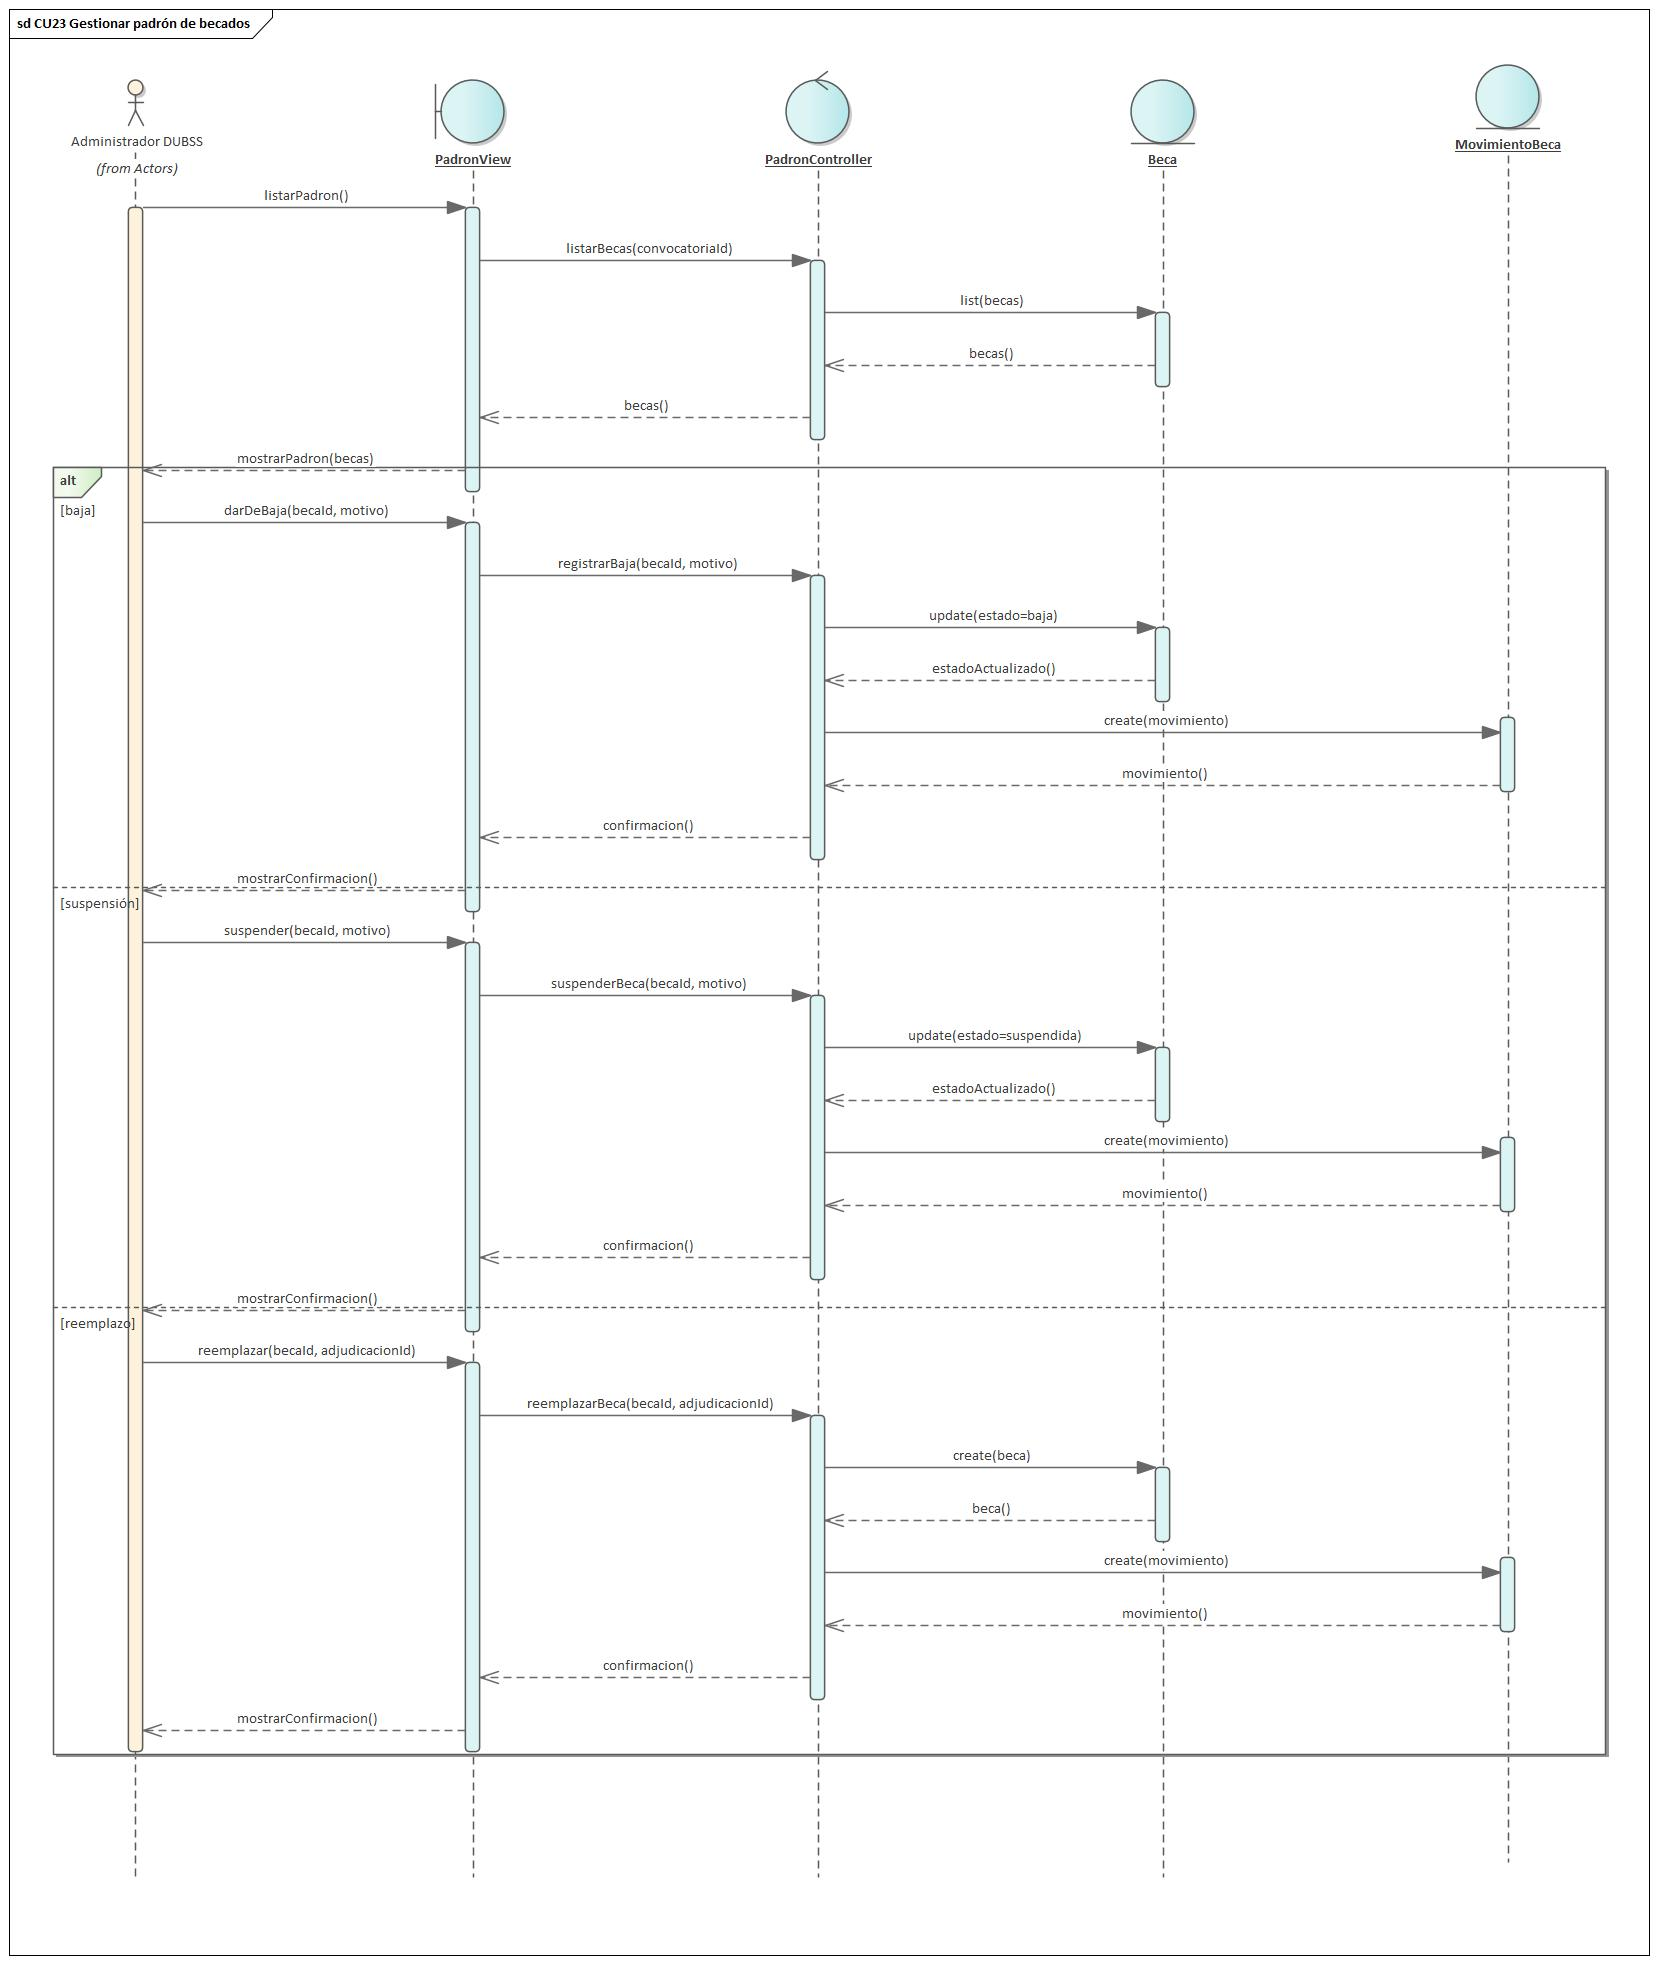
\includegraphics[width=\textwidth,height=0.75\textheight,keepaspectratio]{images/103_Secuencia_CU23_Gestionar_Padron_Becados.jpg}

\smallskip
\noindent\raggedright\textit{Nota.} Elaboración propia.
\end{figure}


\Needspace{0.9\textheight}
\subsubsection{7.4.24. Diseñar CU-24 Consultar historial de asistencia y estado de beca}\label{sec:cap7_disenar_cu24}

La Figura~\ref{fig:secuencia_cu24} presenta el diagrama de secuencia del CU-24.

\begin{figure}[H]
\caption{Diagrama de secuencia del CU-24 Consultar historial de asistencia y estado de beca}
\label{fig:secuencia_cu24}
\centering
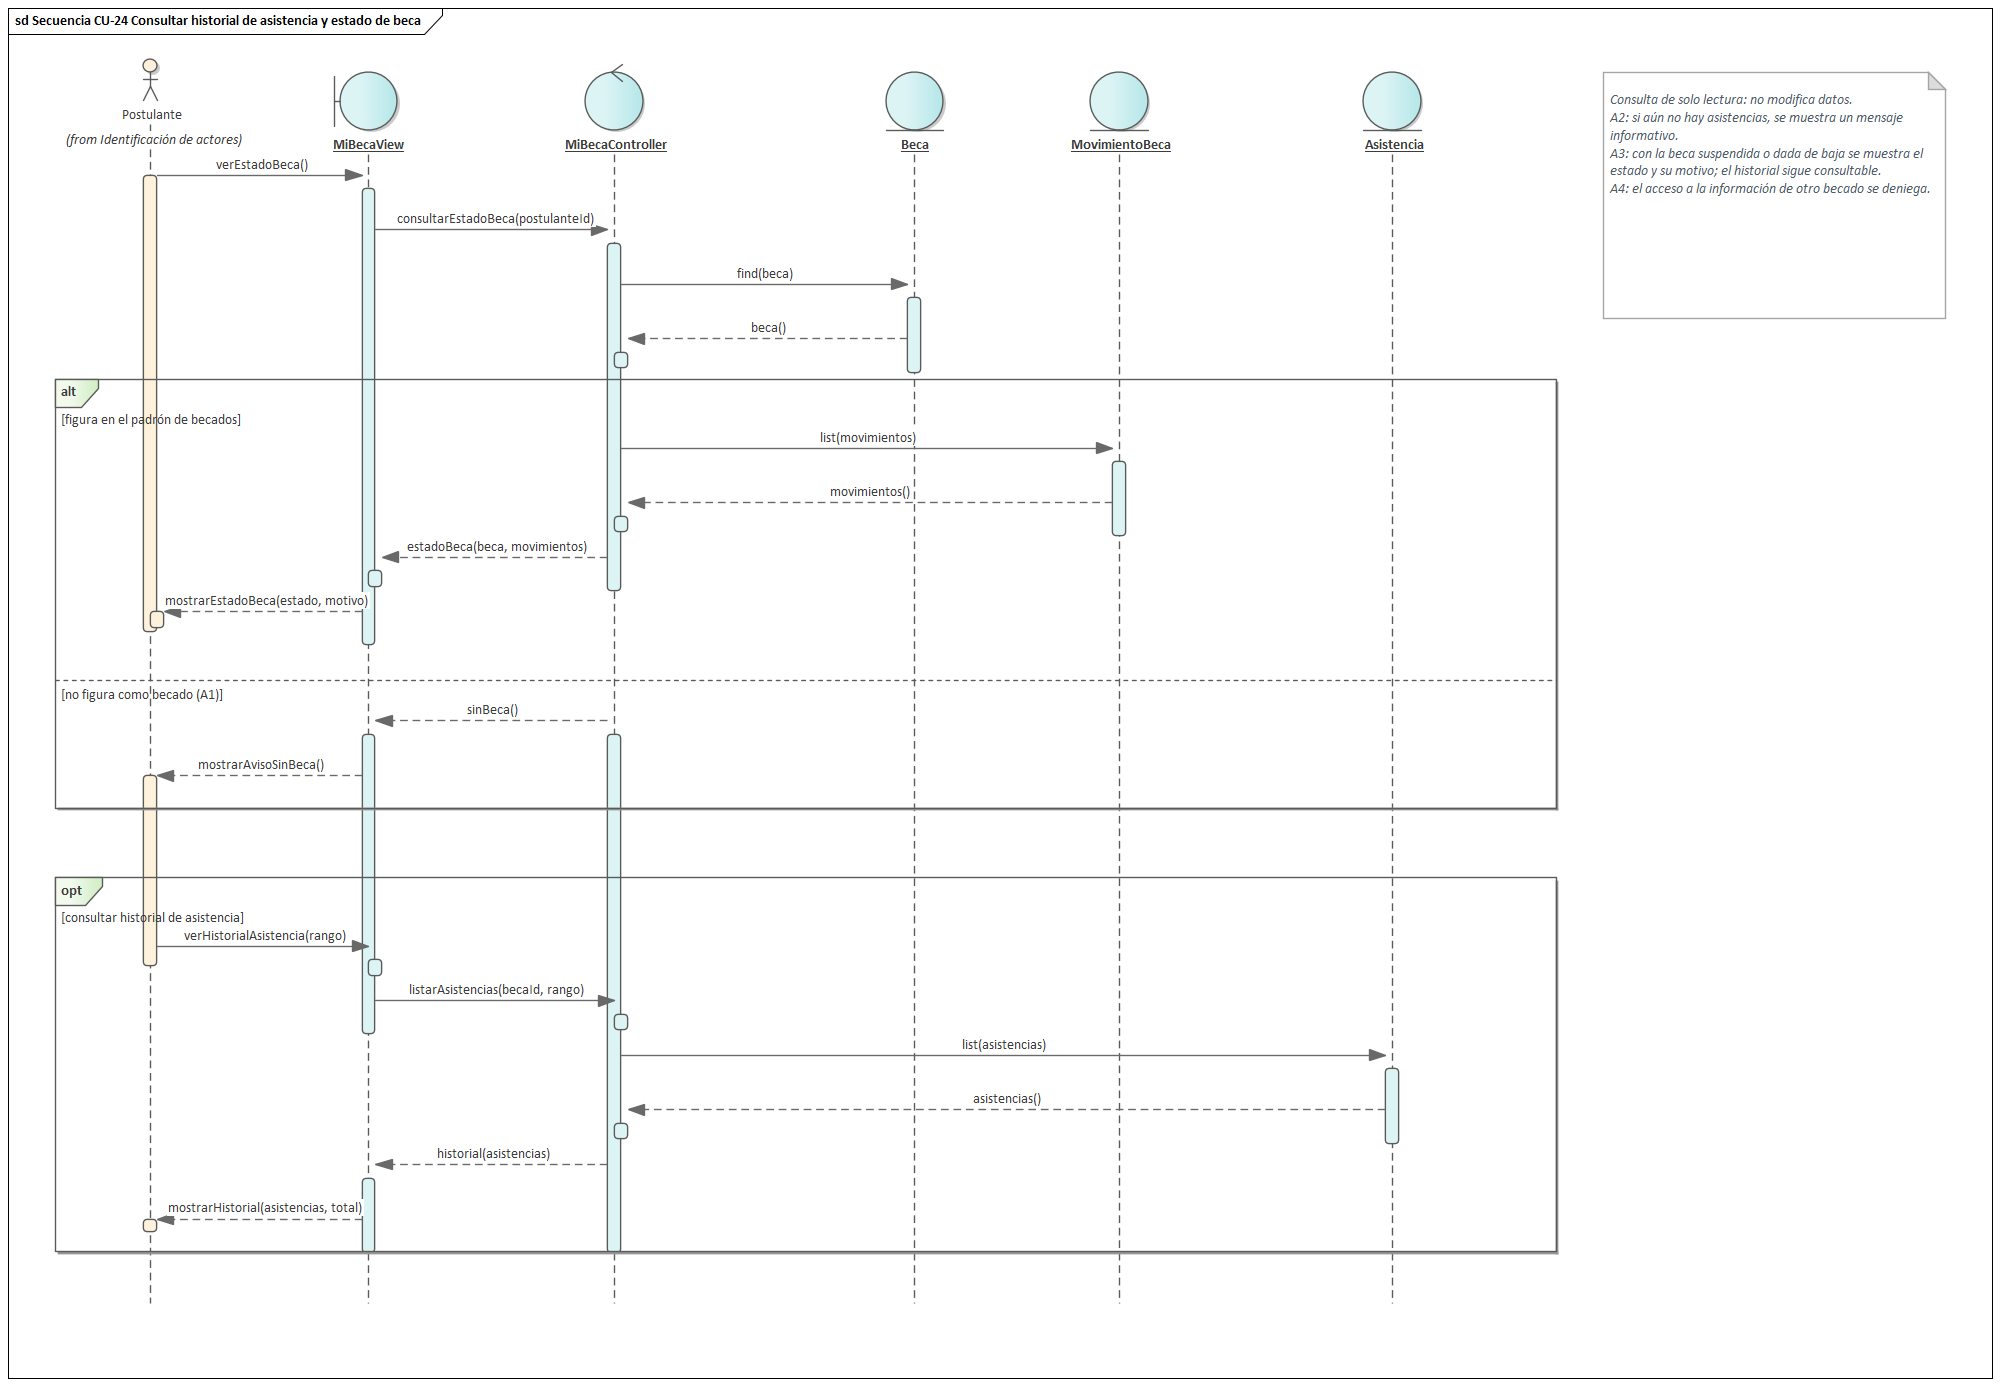
\includegraphics[width=\textwidth,height=0.75\textheight,keepaspectratio]{images/132_Secuencia_CU24_Consultar_Historial_Asistencia_Beca.png}

\smallskip
\noindent\raggedright\textit{Nota.} Elaboración propia.
\end{figure}


\Needspace{0.9\textheight}
\subsubsection{7.4.25. Diseñar CU-25 Consultar bitácora de acciones}\label{sec:cap7_disenar_cu25}

La Figura~\ref{fig:secuencia_cu25} presenta el diagrama de secuencia del CU-25.

\begin{figure}[H]
\caption{Diagrama de secuencia del CU-25 Consultar bitácora de acciones}
\label{fig:secuencia_cu25}
\centering
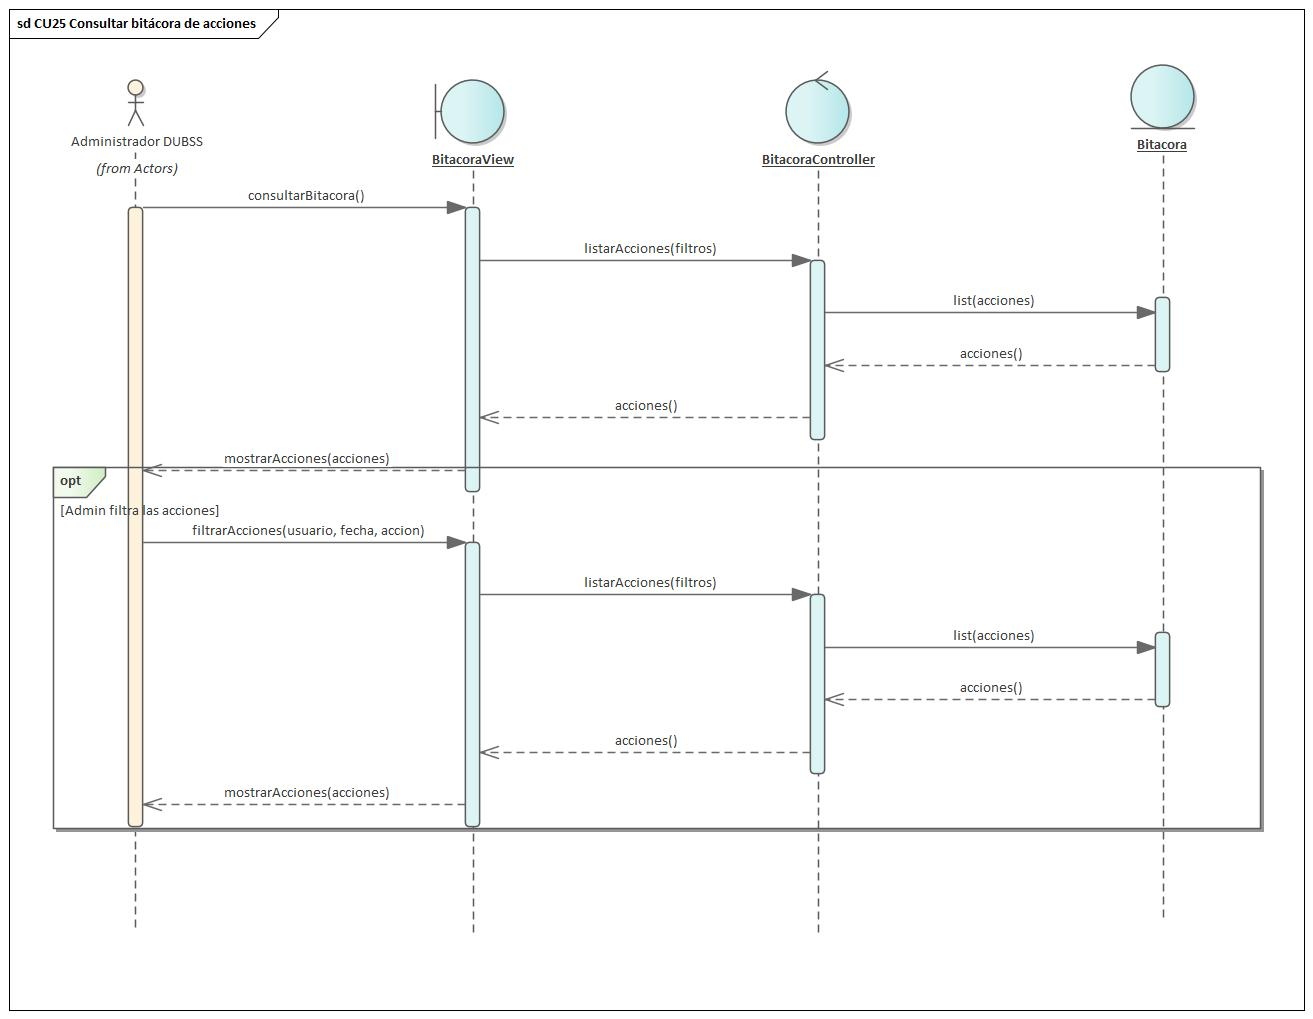
\includegraphics[width=\textwidth,height=0.75\textheight,keepaspectratio]{images/104_Secuencia_CU25_Consultar_Bitacora_Acciones.jpg}

\smallskip
\noindent\raggedright\textit{Nota.} Elaboración propia.
\end{figure}


\Needspace{0.9\textheight}
\subsubsection{7.4.26. Diseñar CU-26 Parametrizar modelo de preselección y reprocesar puntajes}\label{sec:cap7_disenar_cu26}

La Figura~\ref{fig:secuencia_cu26} presenta el diagrama de secuencia del CU-26.

\begin{figure}[H]
\caption{Diagrama de secuencia del CU-26 Parametrizar modelo de preselección y reprocesar puntajes}
\label{fig:secuencia_cu26}
\centering
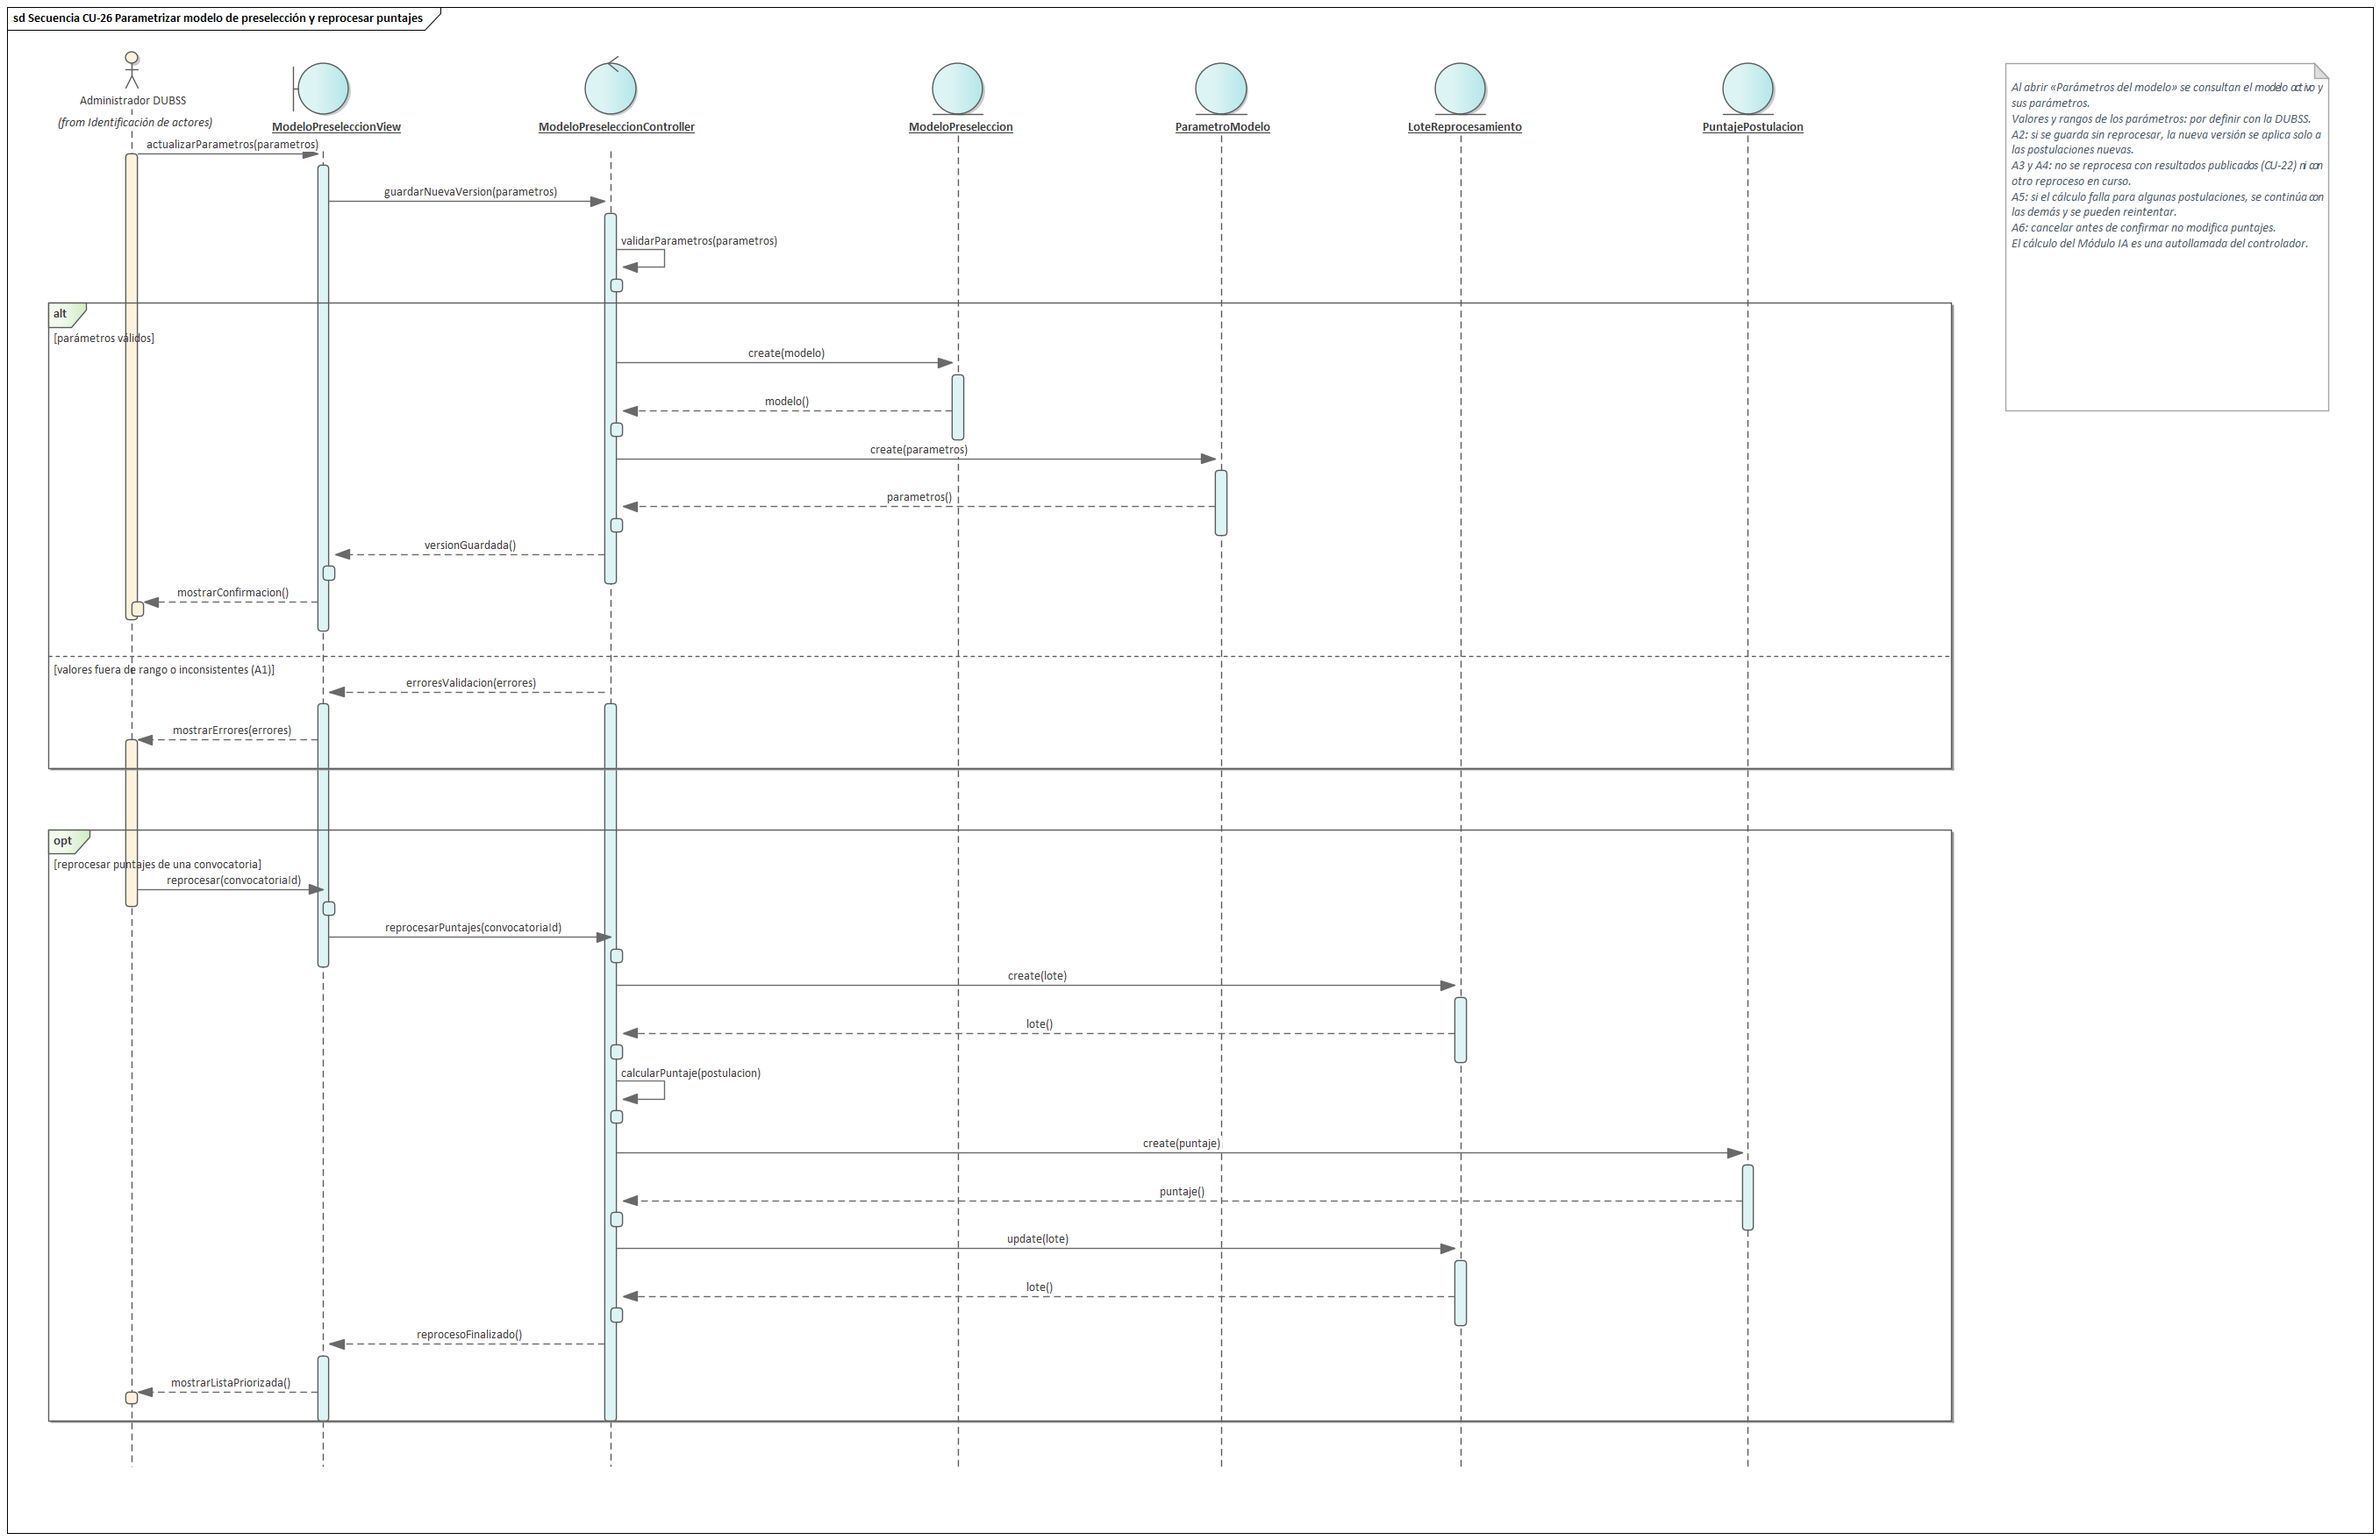
\includegraphics[width=\textwidth,height=0.75\textheight,keepaspectratio]{images/133_Secuencia_CU26_Parametrizar_Modelo_Preseleccion.png}

\smallskip
\noindent\raggedright\textit{Nota.} Elaboración propia.
\end{figure}


% ------------------------------------------------------------------------------
% 7.5. DISEÑO DE INTERFACES
% ------------------------------------------------------------------------------
\wfa{\wn{7}.5. Diseño de Interfaces}\label{sec:cap7_diseno_interfaces}

El diseño de interfaces expresa, mediante maquetas (\textit{mockups}), la disposición de los elementos visuales con los que el actor interactúa en cada caso de uso, de modo que las clases de interfaz (\textit{View}) identificadas en el análisis cuenten con una representación concreta \parencite{jacobson1999unified}.

A continuación se presenta el diseño de interfaces de los veintiséis casos de uso del sistema, en el orden de su numeración (CU-01 a CU-26).

\Needspace{0.9\textheight}
\wfb{\wn{7}.5.1. Interfaz CU-01 Registrarse y autenticarse}\label{sec:cap7_interfaz_cu01}

La Figura~\ref{fig:mockup_cu01} presenta la maqueta de interfaz del CU-01.

\begin{figure}[H]
\caption{Maqueta de interfaz del CU-01 Registrarse y autenticarse}
\label{fig:mockup_cu01}
\centering
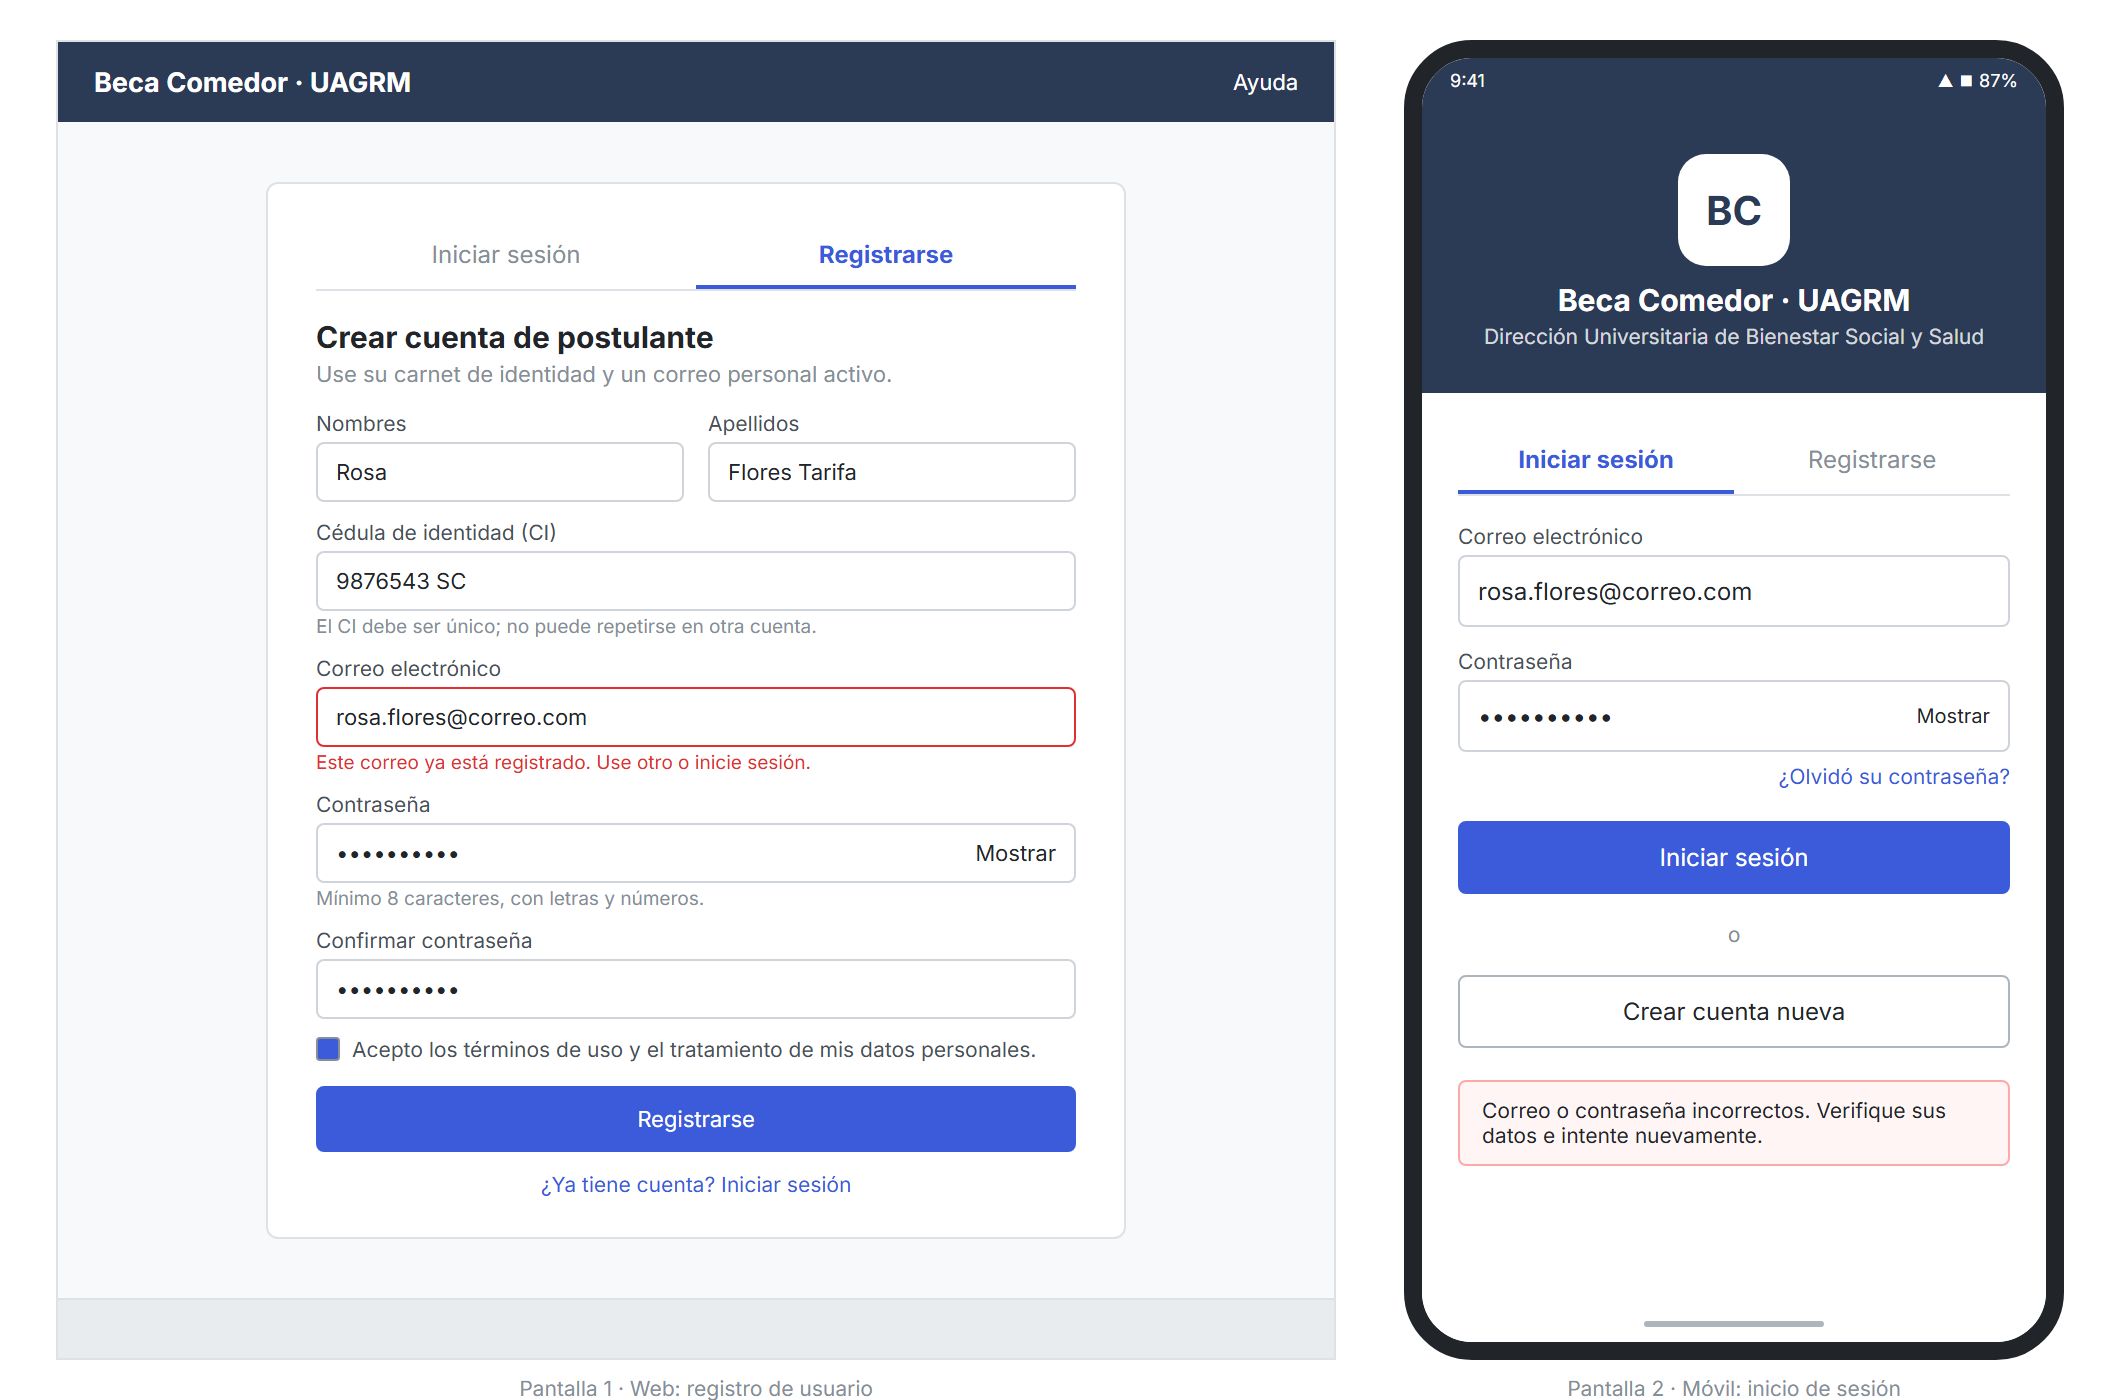
\includegraphics[width=\textwidth,height=0.75\textheight,keepaspectratio]{images/134_Mockup_CU01_Registrarse_autenticarse.png}

\smallskip
\noindent\raggedright\textit{Nota.} Elaboración propia.
\end{figure}



\Needspace{0.9\textheight}
\wfb{\wn{7}.5.2. Interfaz CU-02 Enviar postulación a Beca Comedor}\label{sec:cap7_interfaz_cu02}

La Figura~\ref{fig:mockup_cu02} presenta la maqueta de interfaz del CU-02.

\begin{figure}[H]
\caption{Maqueta de interfaz del CU-02 Enviar postulación a Beca Comedor}
\label{fig:mockup_cu02}
\centering
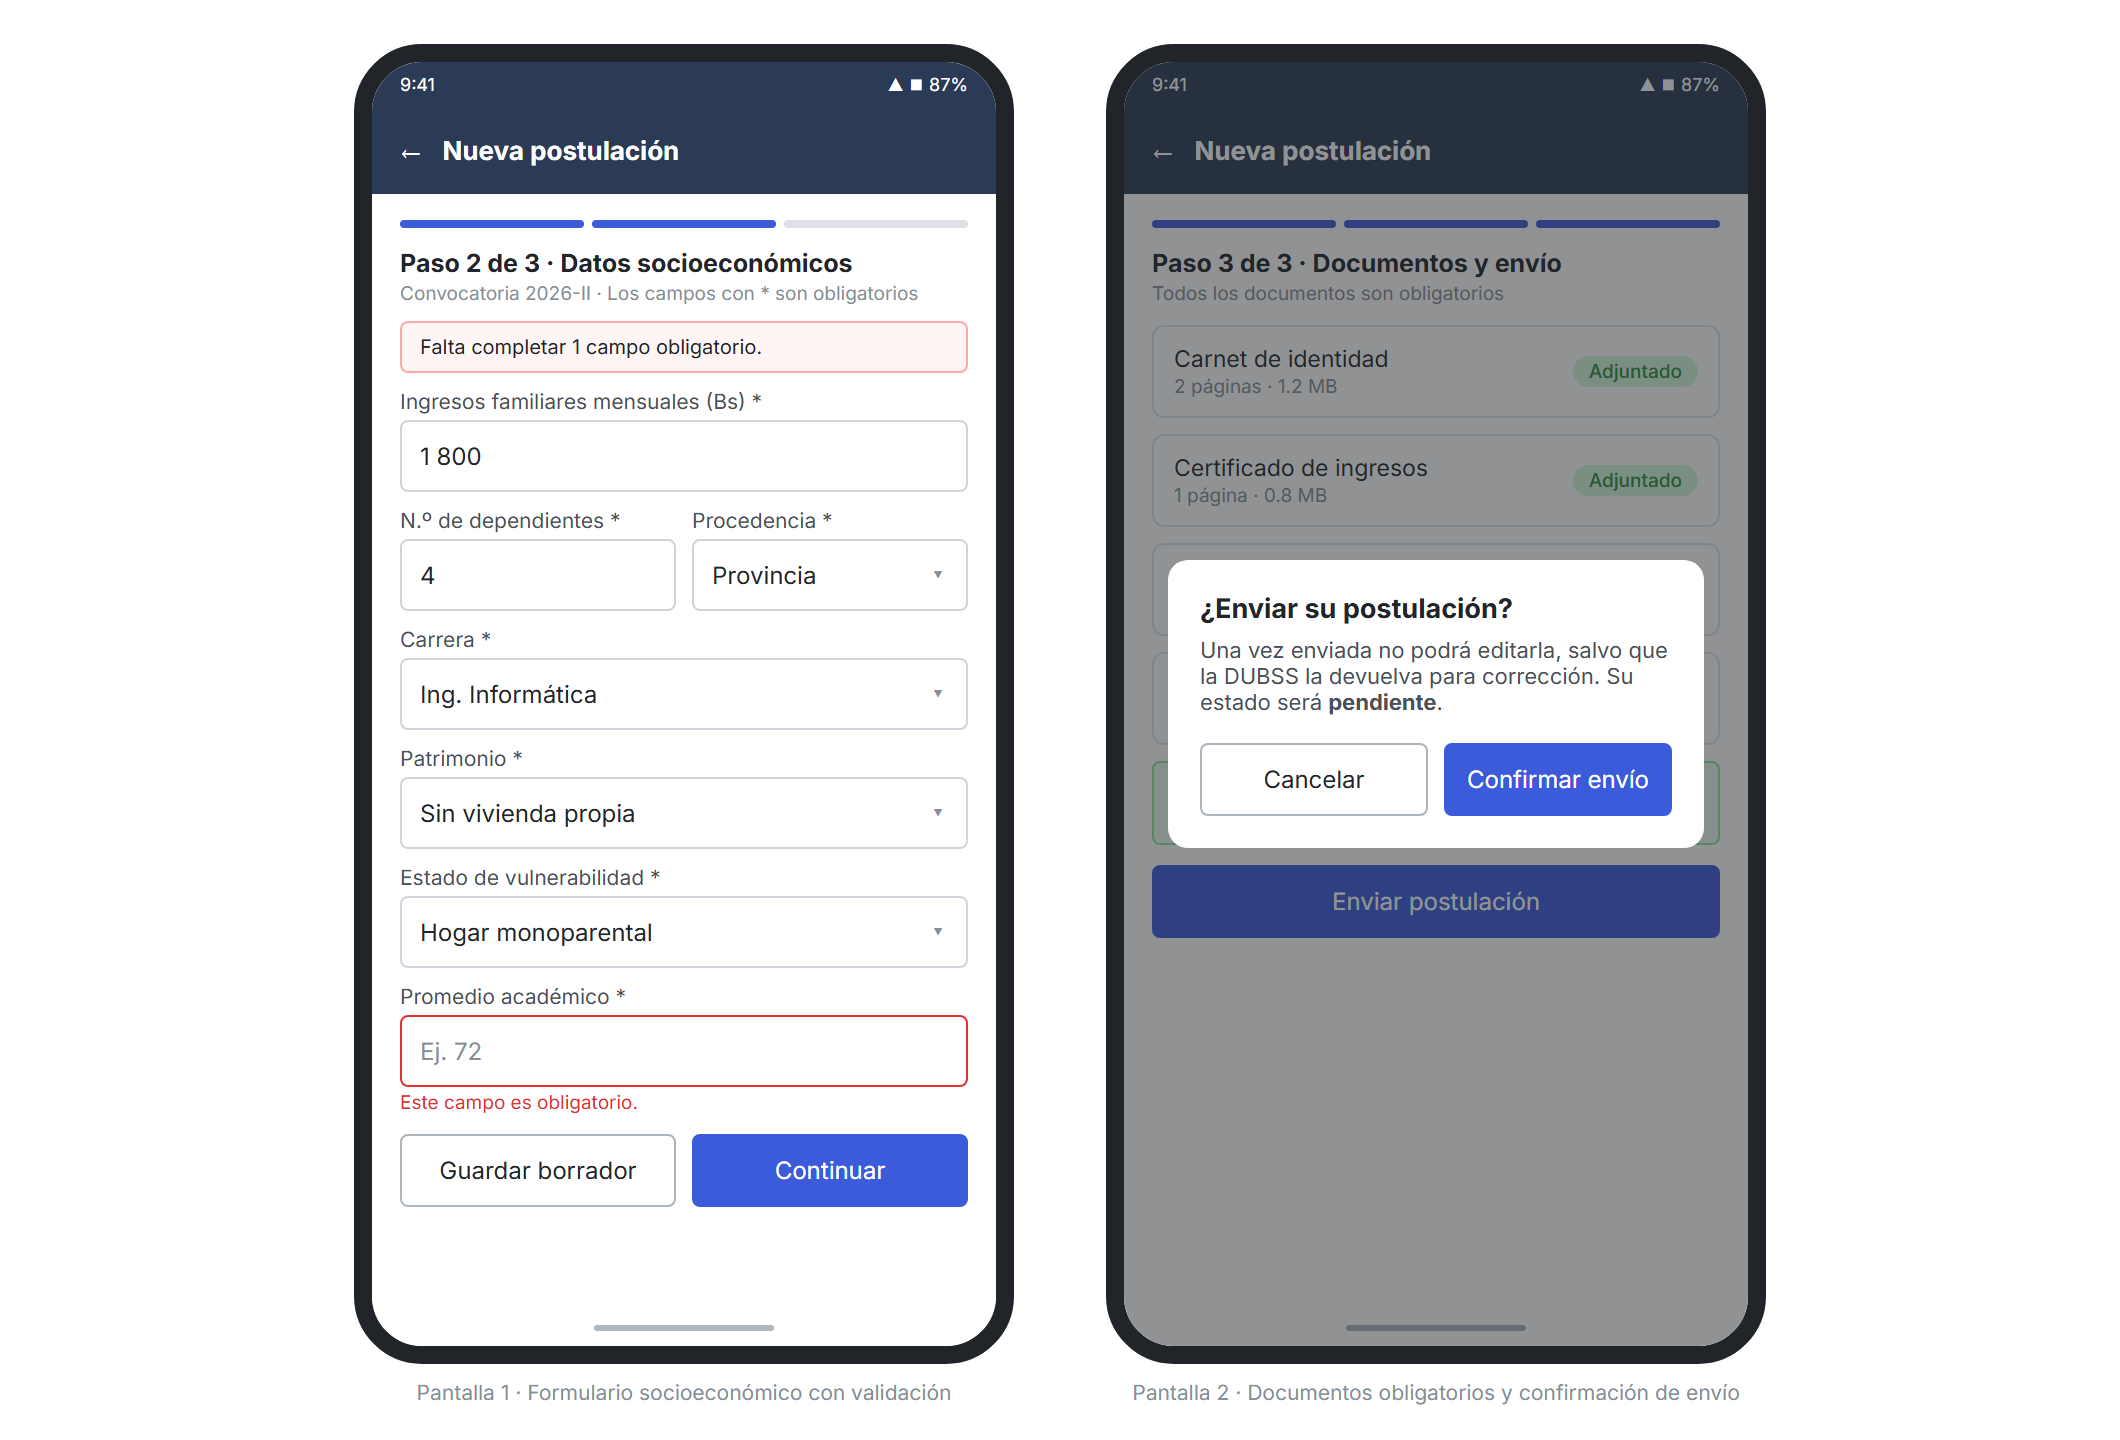
\includegraphics[width=\textwidth,height=0.75\textheight,keepaspectratio]{images/135_Mockup_CU02_Enviar_postulacion.png}

\smallskip
\noindent\raggedright\textit{Nota.} Elaboración propia.
\end{figure}



\Needspace{0.9\textheight}
\wfb{\wn{7}.5.3. Interfaz CU-03 Precalificar postulación con Inteligencia Artificial}\label{sec:cap7_interfaz_cu03}

La Figura~\ref{fig:mockup_cu03} presenta la maqueta de interfaz del CU-03.

\begin{figure}[H]
\caption{Maqueta de interfaz del CU-03 Precalificar postulación con Inteligencia Artificial}
\label{fig:mockup_cu03}
\centering
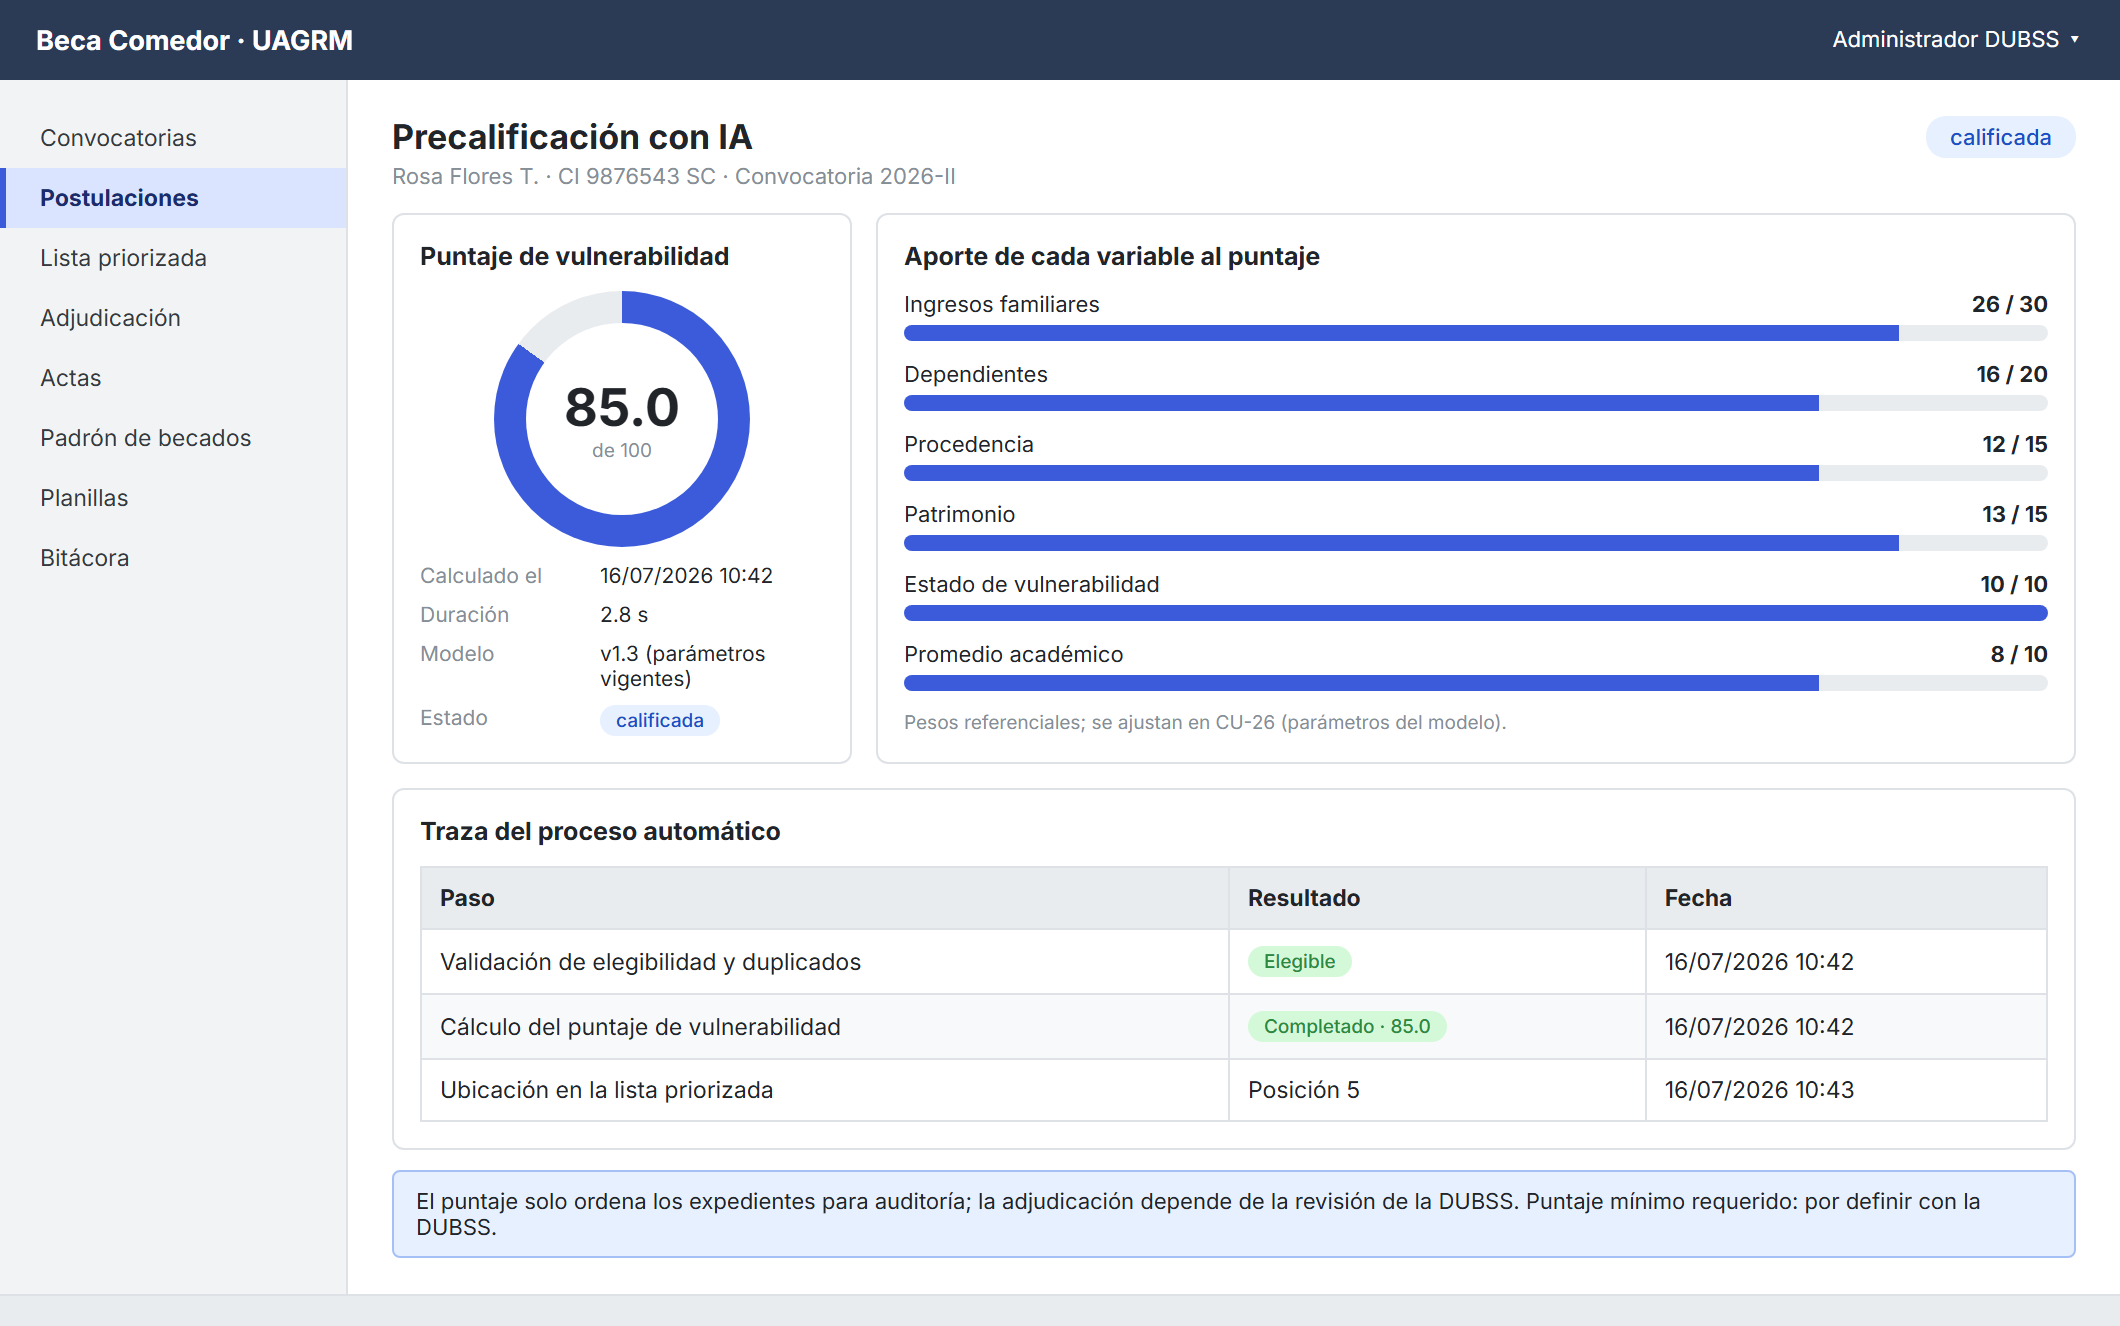
\includegraphics[width=\textwidth,height=0.75\textheight,keepaspectratio]{images/136_Mockup_CU03_Precalificar_IA.png}

\smallskip
\noindent\raggedright\textit{Nota.} Elaboración propia.
\end{figure}



\Needspace{0.9\textheight}
\wfb{\wn{7}.5.4. Interfaz CU-04 Consultar estado de postulación}\label{sec:cap7_interfaz_cu04}

La Figura~\ref{fig:mockup_cu04} presenta la maqueta de interfaz del CU-04.

\begin{figure}[H]
\caption{Maqueta de interfaz del CU-04 Consultar estado de postulación}
\label{fig:mockup_cu04}
\centering
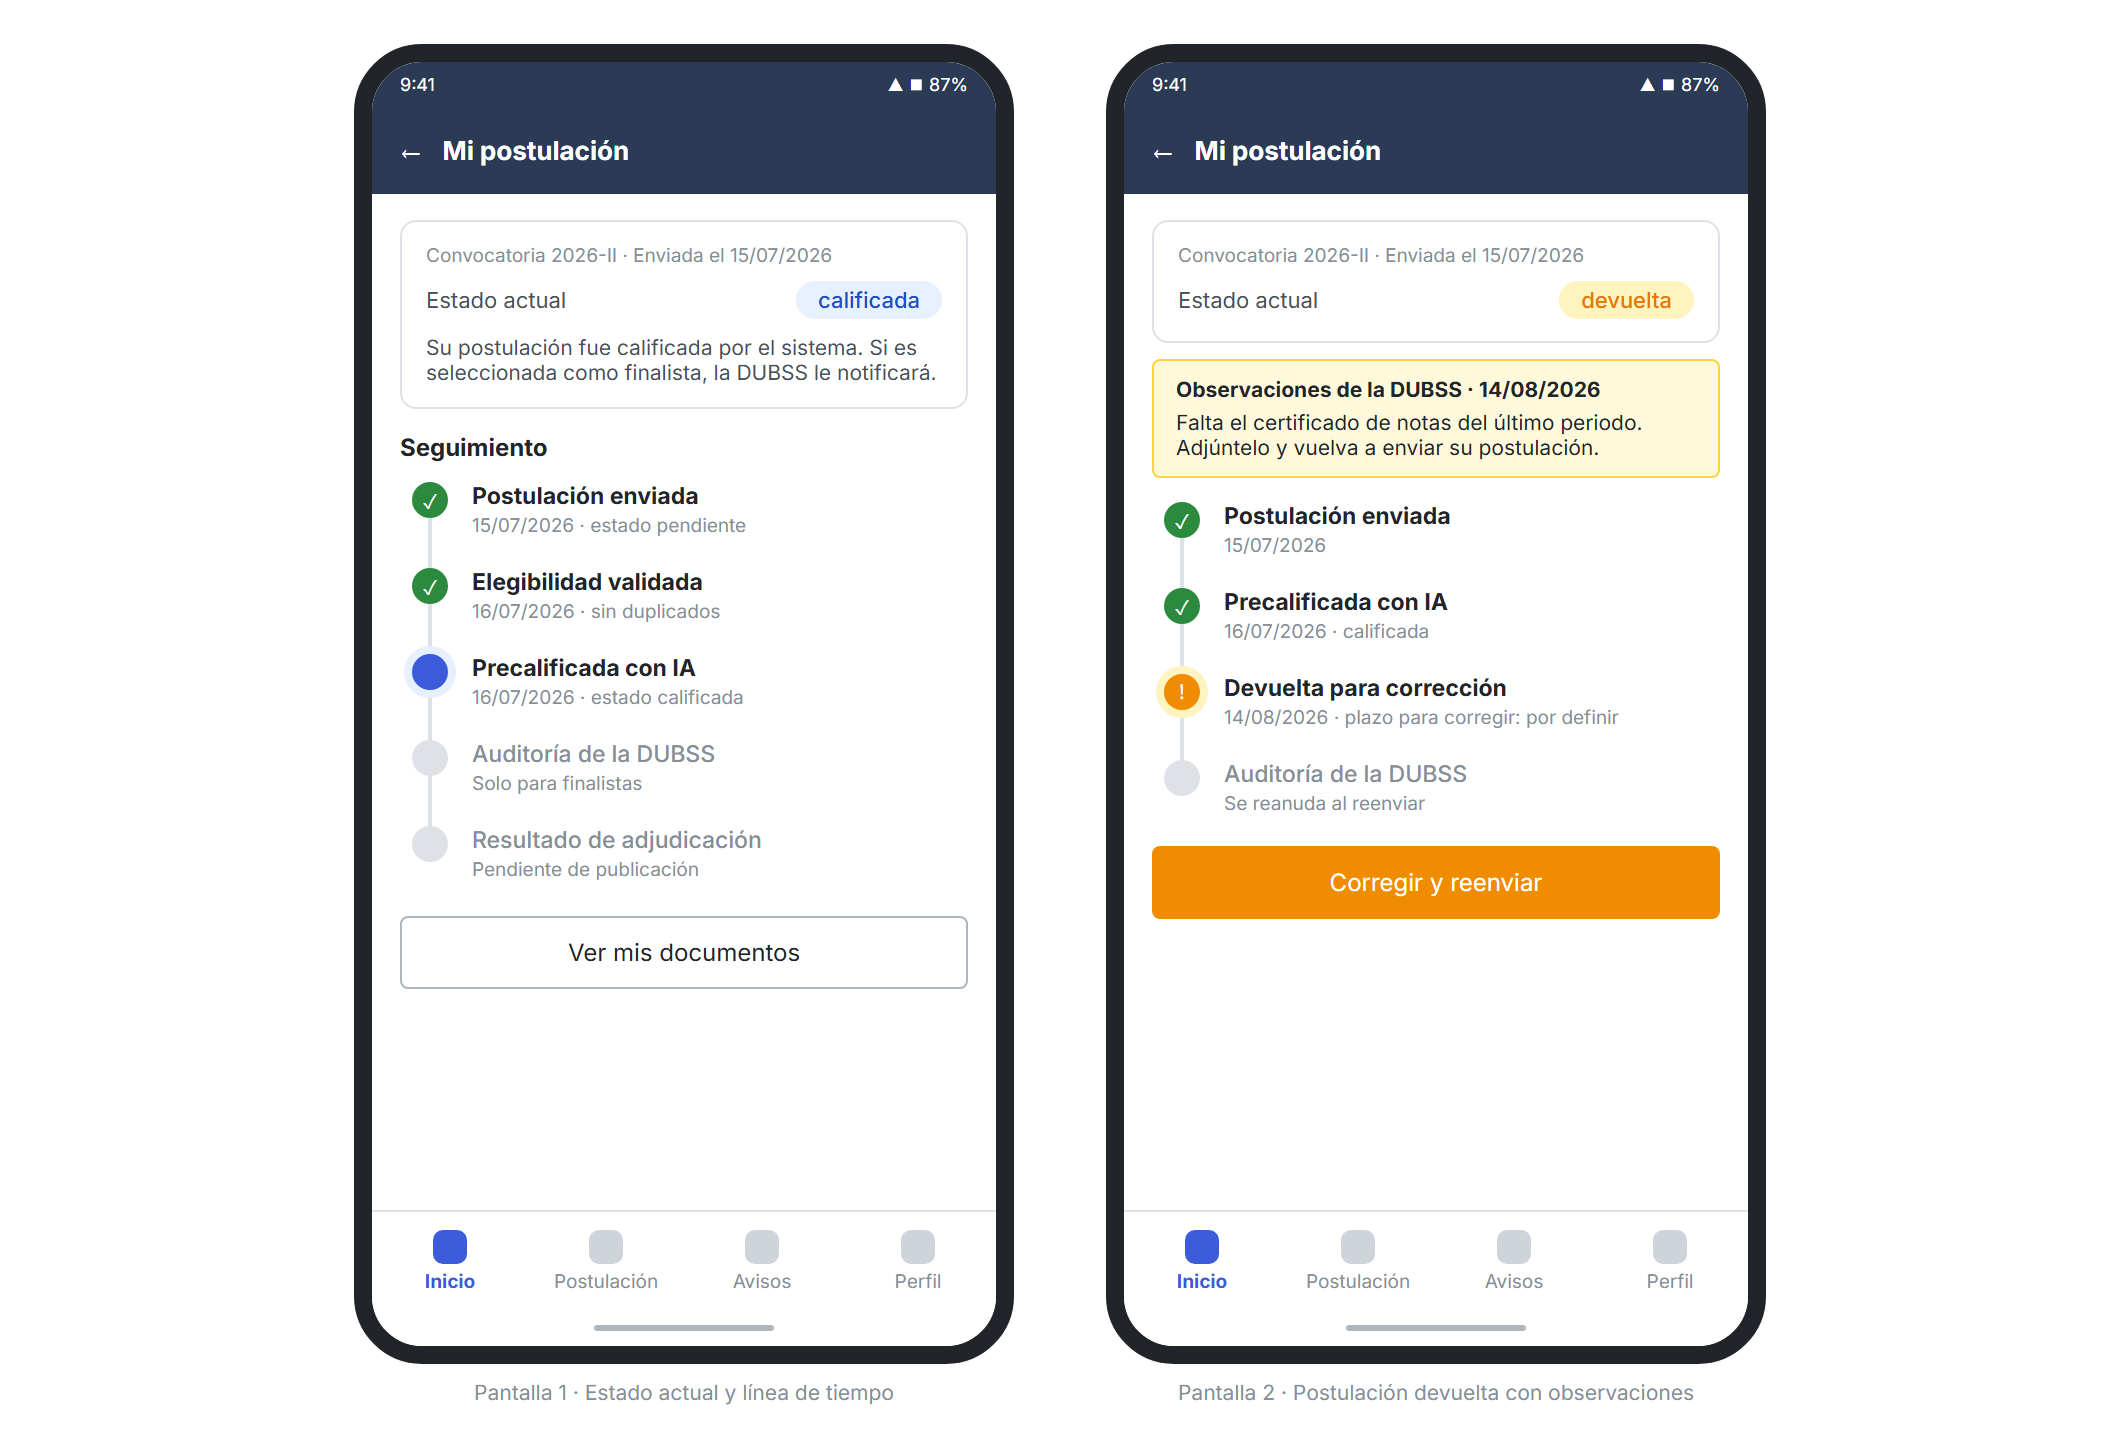
\includegraphics[width=\textwidth,height=0.75\textheight,keepaspectratio]{images/137_Mockup_CU04_Consultar_estado.png}

\smallskip
\noindent\raggedright\textit{Nota.} Elaboración propia.
\end{figure}



\Needspace{0.9\textheight}
\wfb{\wn{7}.5.5. Interfaz CU-05 Auditar y adjudicar becas}\label{sec:cap7_interfaz_cu05}

La Figura~\ref{fig:mockup_cu05} presenta la maqueta de interfaz del CU-05.

\begin{figure}[H]
\caption{Maqueta de interfaz del CU-05 Auditar y adjudicar becas}
\label{fig:mockup_cu05}
\centering
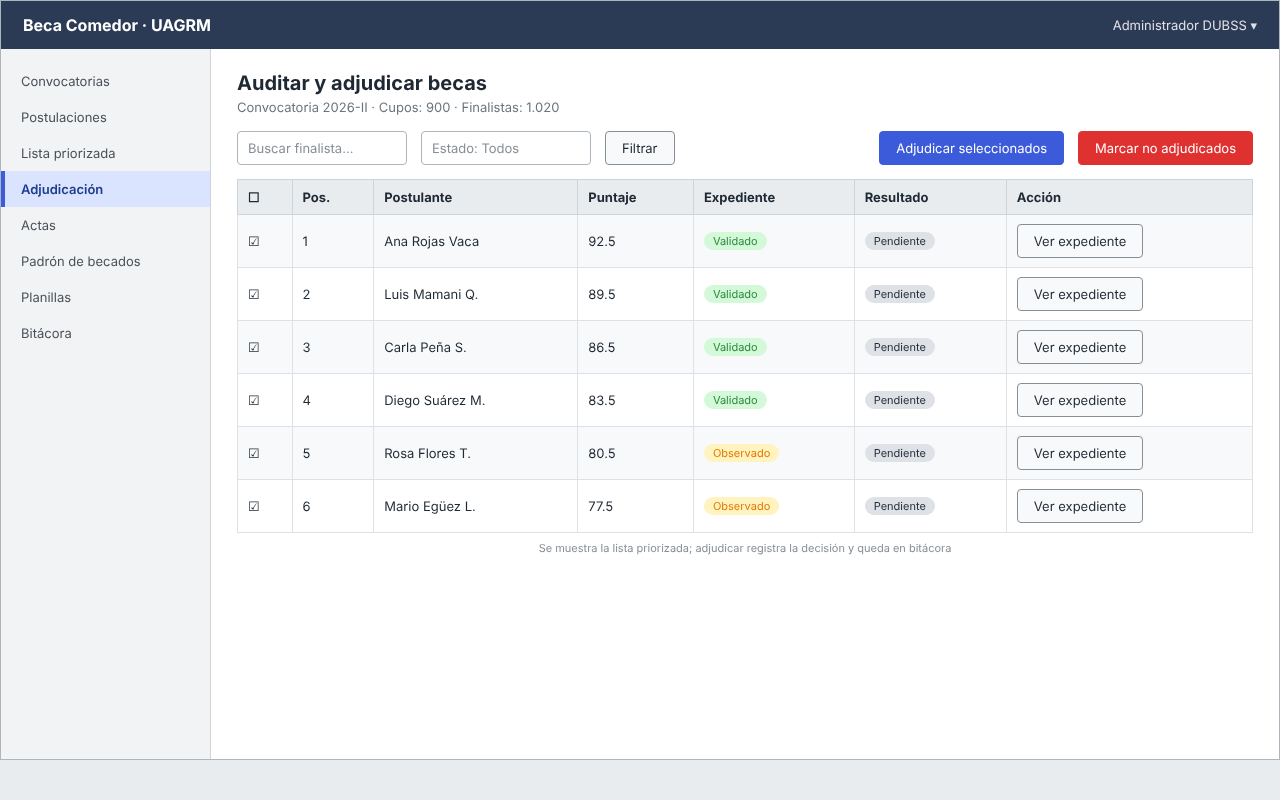
\includegraphics[width=\textwidth,height=0.75\textheight,keepaspectratio]{images/105_Mockup_CU05_Auditar_y_adjudicar_becas.png}

\smallskip
\noindent\raggedright\textit{Nota.} Elaboración propia.
\end{figure}


\Needspace{0.9\textheight}
\wfb{\wn{7}.5.6. Interfaz CU-06 Visualizar lista priorizada de postulantes}\label{sec:cap7_interfaz_cu06}

La Figura~\ref{fig:mockup_cu06} presenta la maqueta de interfaz del CU-06.

\begin{figure}[H]
\caption{Maqueta de interfaz del CU-06 Visualizar lista priorizada de postulantes}
\label{fig:mockup_cu06}
\centering
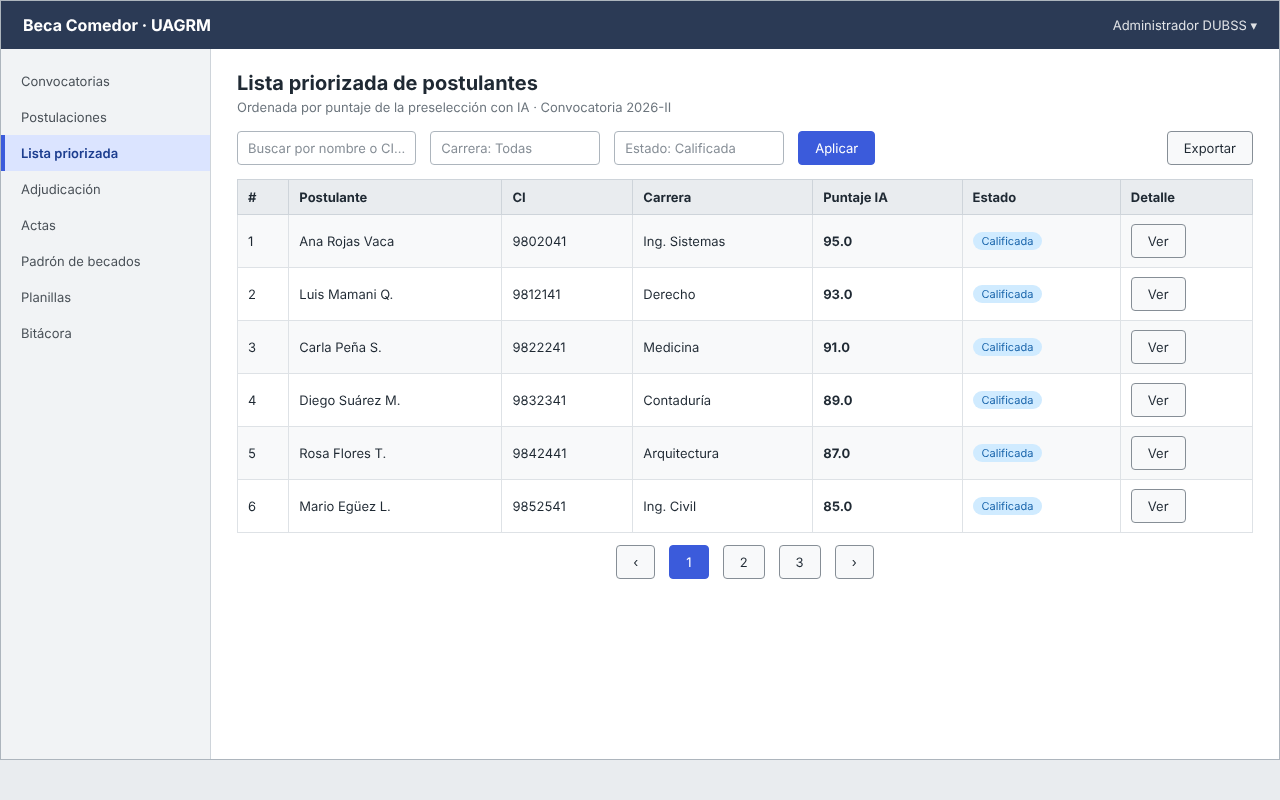
\includegraphics[width=\textwidth,height=0.75\textheight,keepaspectratio]{images/106_Mockup_CU06_Lista_priorizada.png}

\smallskip
\noindent\raggedright\textit{Nota.} Elaboración propia.
\end{figure}


\Needspace{0.9\textheight}
\wfb{\wn{7}.5.7. Interfaz CU-07 Auditar expediente finalista}\label{sec:cap7_interfaz_cu07}

La Figura~\ref{fig:mockup_cu07} presenta la maqueta de interfaz del CU-07.

\begin{figure}[H]
\caption{Maqueta de interfaz del CU-07 Auditar expediente finalista}
\label{fig:mockup_cu07}
\centering
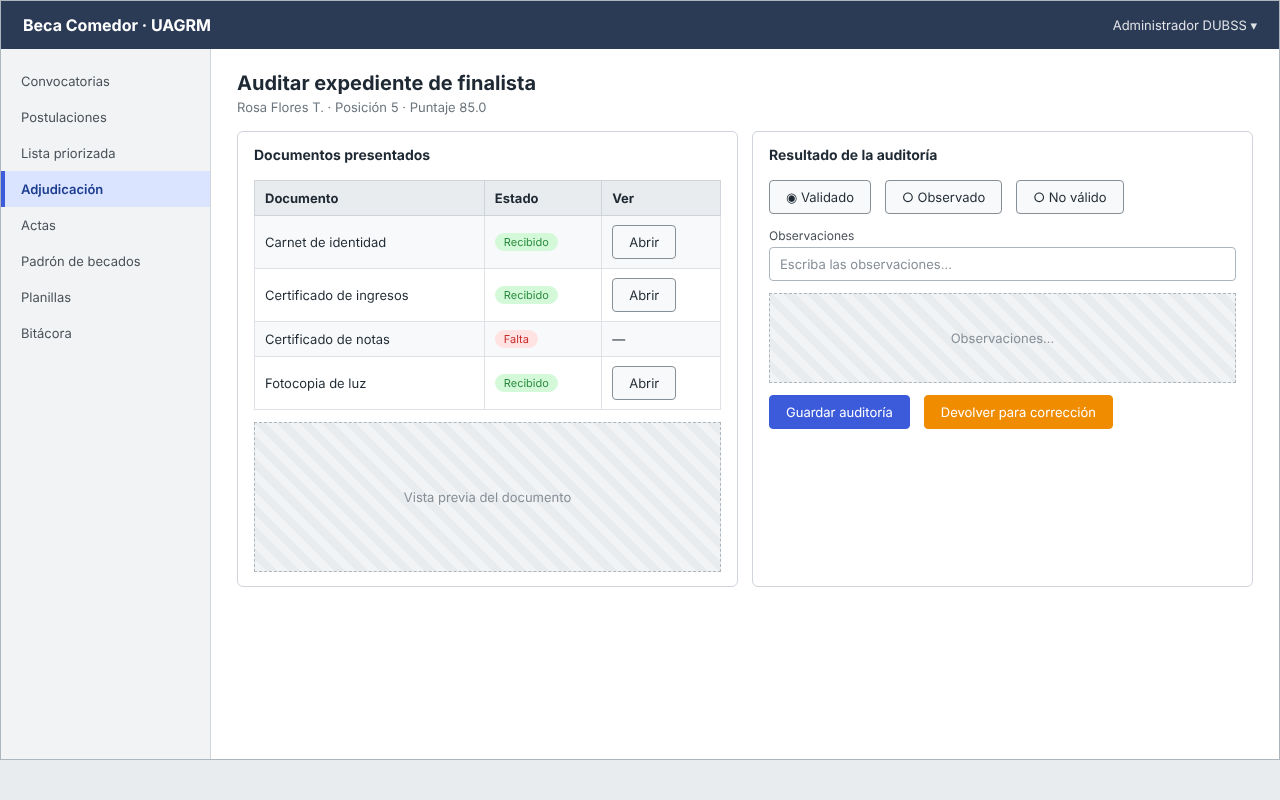
\includegraphics[width=\textwidth,height=0.75\textheight,keepaspectratio]{images/107_Mockup_CU07_Auditar_expediente_finalista.png}

\smallskip
\noindent\raggedright\textit{Nota.} Elaboración propia.
\end{figure}


\Needspace{0.9\textheight}
\wfb{\wn{7}.5.8. Interfaz CU-08 Generar acta de adjudicación}\label{sec:cap7_interfaz_cu08}

La Figura~\ref{fig:mockup_cu08} presenta la maqueta de interfaz del CU-08.

\begin{figure}[H]
\caption{Maqueta de interfaz del CU-08 Generar acta de adjudicación}
\label{fig:mockup_cu08}
\centering
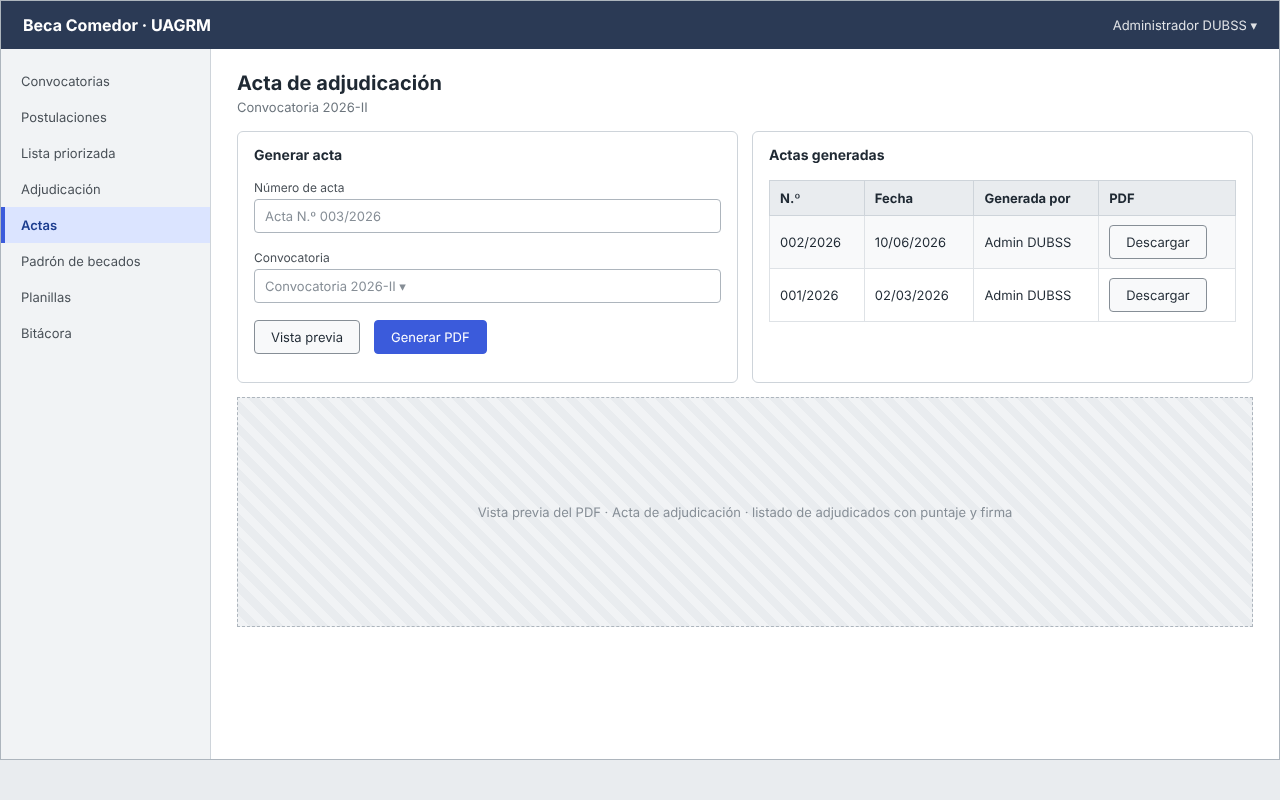
\includegraphics[width=\textwidth,height=0.75\textheight,keepaspectratio]{images/108_Mockup_CU08_Acta_de_adjudicacion.png}

\smallskip
\noindent\raggedright\textit{Nota.} Elaboración propia.
\end{figure}


\Needspace{0.9\textheight}
\wfb{\wn{7}.5.9. Interfaz CU-09 Generar planilla de asistencia}\label{sec:cap7_interfaz_cu09}

La Figura~\ref{fig:mockup_cu09} presenta la maqueta de interfaz del CU-09.

\begin{figure}[H]
\caption{Maqueta de interfaz del CU-09 Generar planilla de asistencia}
\label{fig:mockup_cu09}
\centering
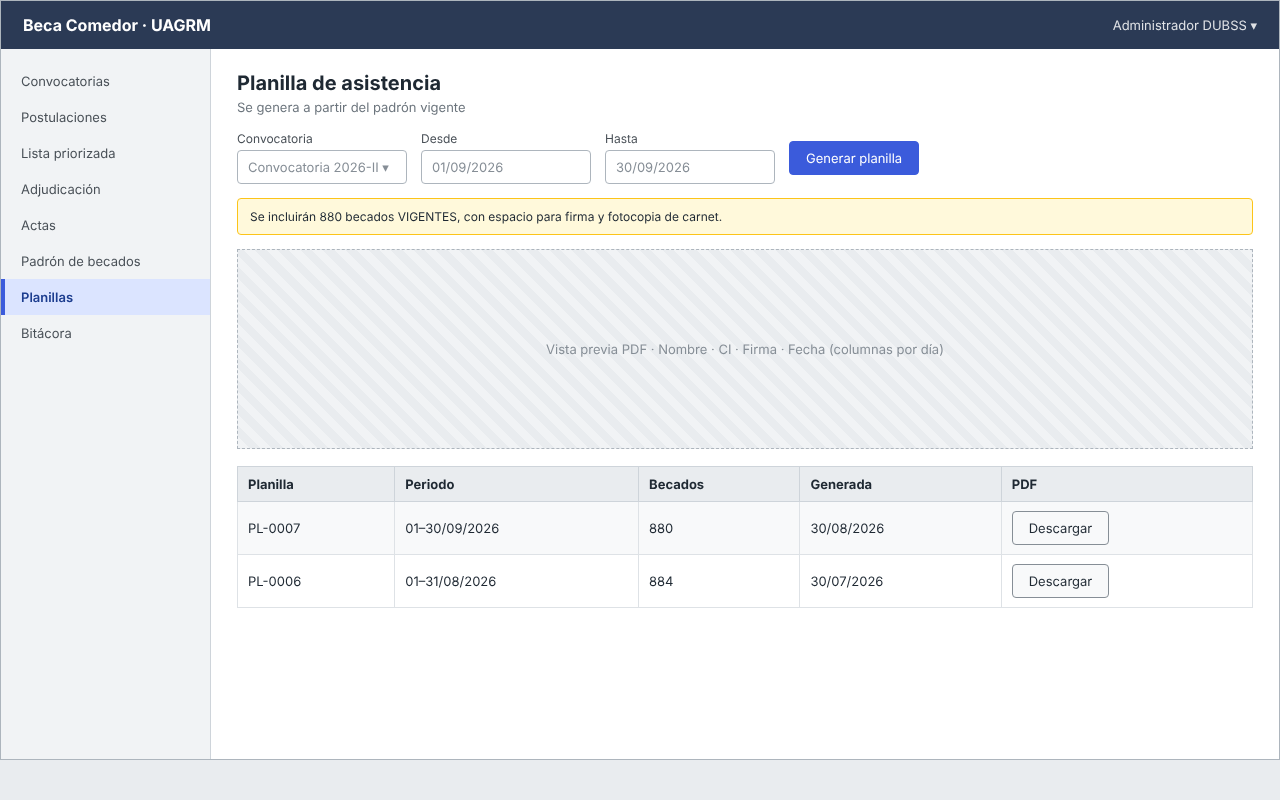
\includegraphics[width=\textwidth,height=0.75\textheight,keepaspectratio]{images/109_Mockup_CU09_Planilla_de_asistencia.png}

\smallskip
\noindent\raggedright\textit{Nota.} Elaboración propia.
\end{figure}


\Needspace{0.9\textheight}
\wfb{\wn{7}.5.10. Interfaz CU-10 Registrar asistencia digital}\label{sec:cap7_interfaz_cu10}

La Figura~\ref{fig:mockup_cu10} presenta la maqueta de interfaz del CU-10.

\begin{figure}[H]
\caption{Maqueta de interfaz del CU-10 Registrar asistencia digital}
\label{fig:mockup_cu10}
\centering
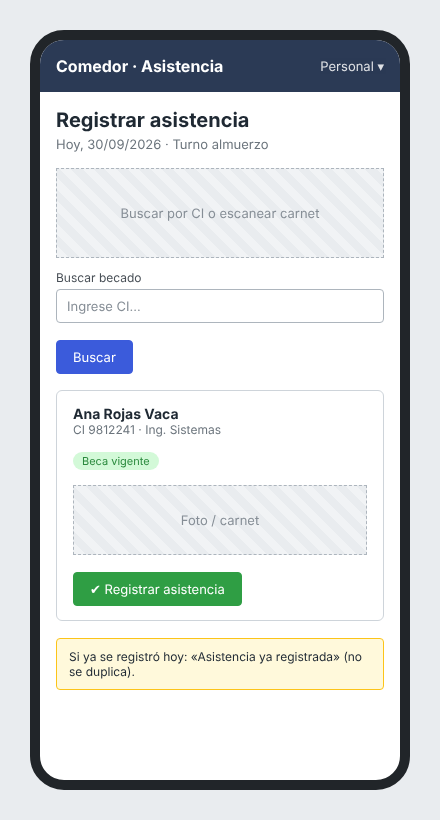
\includegraphics[width=\textwidth,height=0.75\textheight,keepaspectratio]{images/110_Mockup_CU10_Registrar_asistencia_digital.png}

\smallskip
\noindent\raggedright\textit{Nota.} Elaboración propia.
\end{figure}


\Needspace{0.9\textheight}
\wfb{\wn{7}.5.11. Interfaz CU-11 Cotejar registro contra respaldo físico}\label{sec:cap7_interfaz_cu11}

La Figura~\ref{fig:mockup_cu11} presenta la maqueta de interfaz del CU-11.

\begin{figure}[H]
\caption{Maqueta de interfaz del CU-11 Cotejar registro contra respaldo físico}
\label{fig:mockup_cu11}
\centering
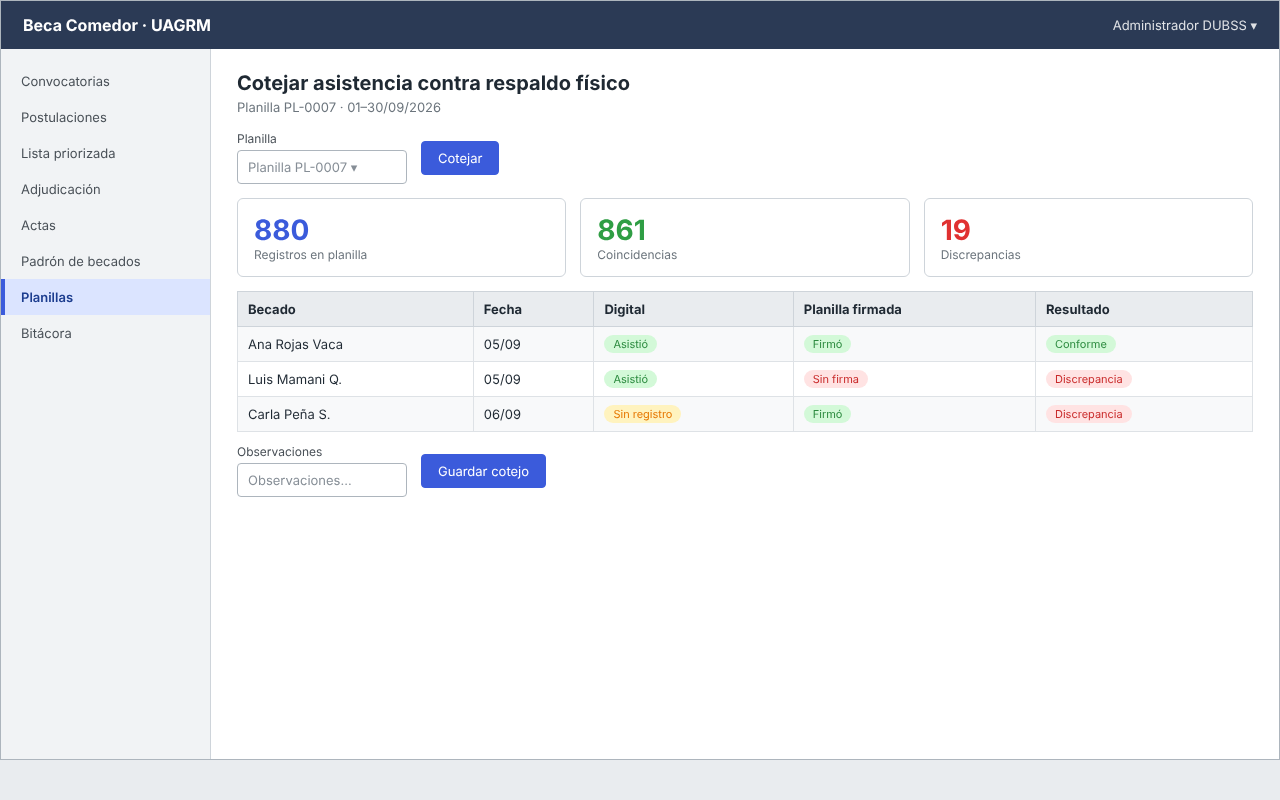
\includegraphics[width=\textwidth,height=0.75\textheight,keepaspectratio]{images/111_Mockup_CU11_Cotejar_contra_respaldo_fisico.png}

\smallskip
\noindent\raggedright\textit{Nota.} Elaboración propia.
\end{figure}


\Needspace{0.9\textheight}
\wfb{\wn{7}.5.12. Interfaz CU-12 Visualizar dashboard de indicadores BI}\label{sec:cap7_interfaz_cu12}

La Figura~\ref{fig:mockup_cu12} presenta la maqueta de interfaz del CU-12.

\begin{figure}[H]
\caption{Maqueta de interfaz del CU-12 Visualizar dashboard de indicadores BI}
\label{fig:mockup_cu12}
\centering
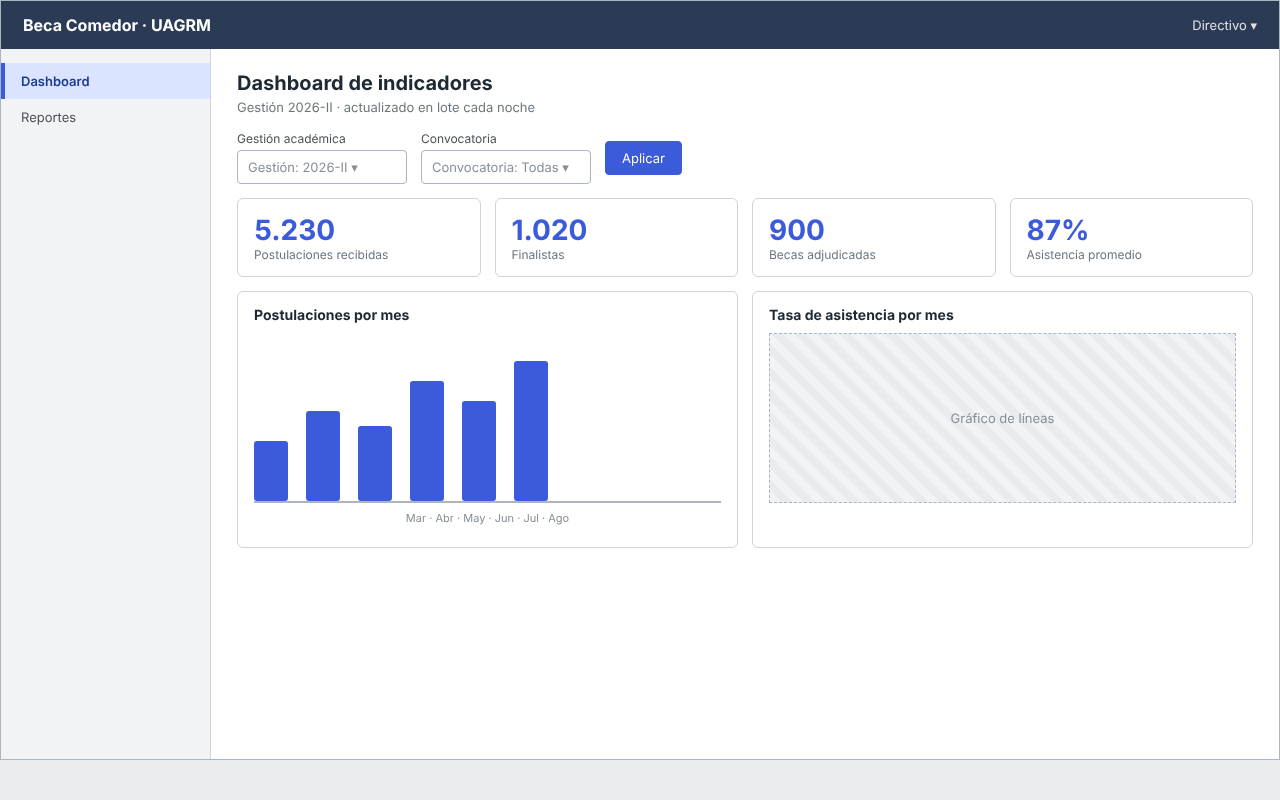
\includegraphics[width=\textwidth,height=0.75\textheight,keepaspectratio]{images/112_Mockup_CU12_Dashboard_BI.png}

\smallskip
\noindent\raggedright\textit{Nota.} Elaboración propia.
\end{figure}


\Needspace{0.9\textheight}
\wfb{\wn{7}.5.13. Interfaz CU-13 Gestionar convocatoria y gestión académica}\label{sec:cap7_interfaz_cu13}

La Figura~\ref{fig:mockup_cu13} presenta la maqueta de interfaz del CU-13.

\begin{figure}[H]
\caption{Maqueta de interfaz del CU-13 Gestionar convocatoria y gestión académica}
\label{fig:mockup_cu13}
\centering
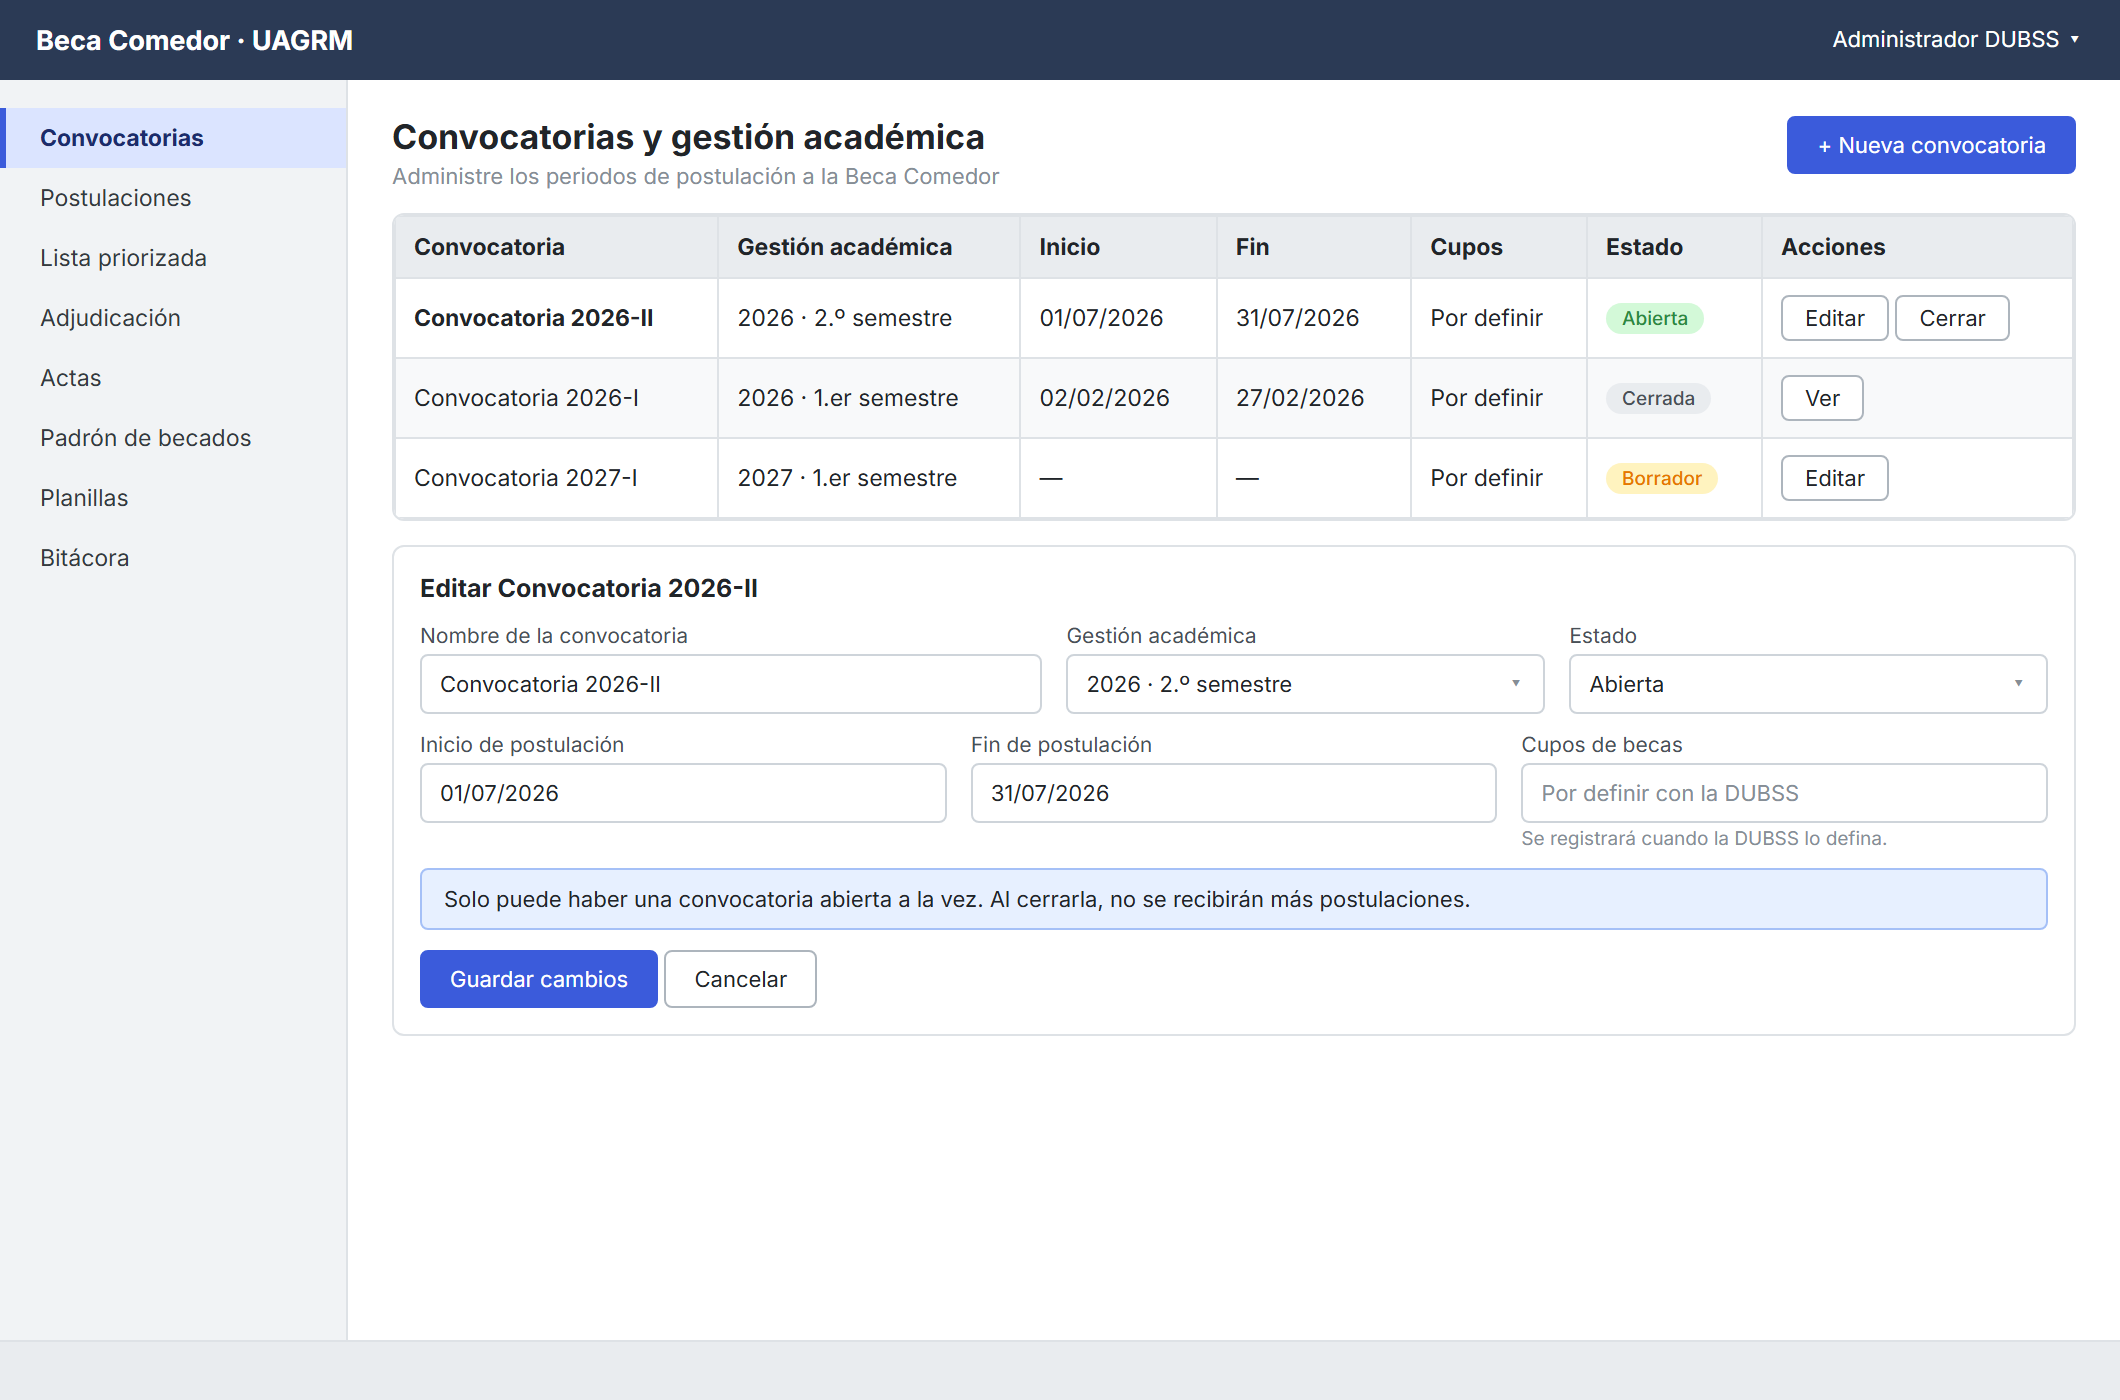
\includegraphics[width=\textwidth,height=0.75\textheight,keepaspectratio]{images/138_Mockup_CU13_Gestionar_convocatoria.png}

\smallskip
\noindent\raggedright\textit{Nota.} Elaboración propia.
\end{figure}



\Needspace{0.9\textheight}
\wfb{\wn{7}.5.14. Interfaz CU-14 Gestionar usuarios y roles}\label{sec:cap7_interfaz_cu14}

La Figura~\ref{fig:mockup_cu14} presenta la maqueta de interfaz del CU-14.

\begin{figure}[H]
\caption{Maqueta de interfaz del CU-14 Gestionar usuarios y roles}
\label{fig:mockup_cu14}
\centering
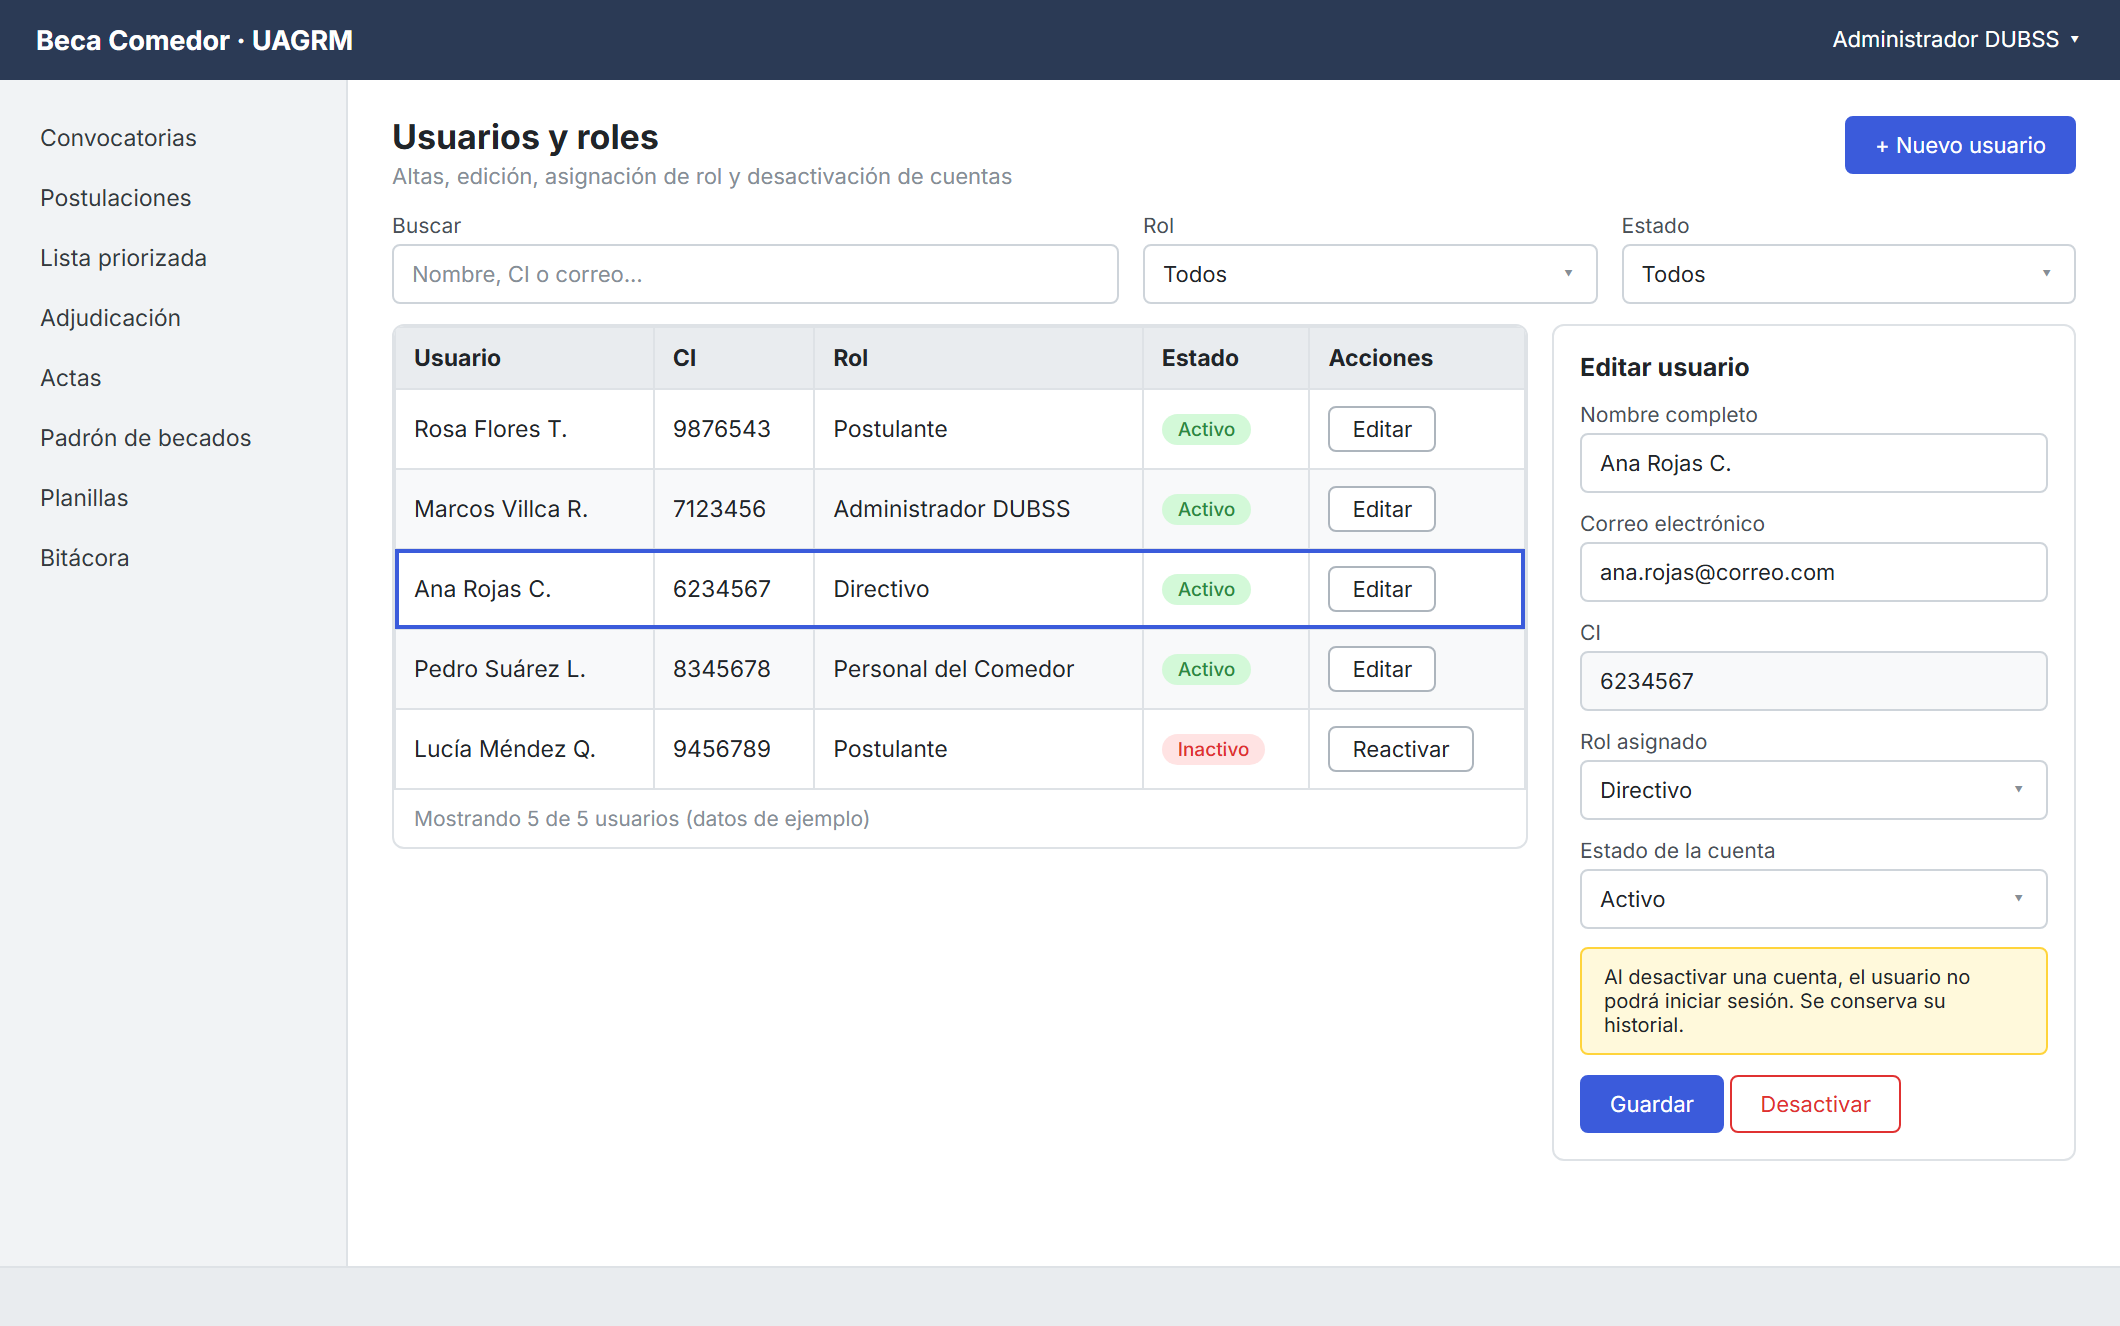
\includegraphics[width=\textwidth,height=0.75\textheight,keepaspectratio]{images/139_Mockup_CU14_Gestionar_usuarios_roles.png}

\smallskip
\noindent\raggedright\textit{Nota.} Elaboración propia.
\end{figure}



\Needspace{0.9\textheight}
\wfb{\wn{7}.5.15. Interfaz CU-15 Recuperar contraseña / gestionar perfil}\label{sec:cap7_interfaz_cu15}

La Figura~\ref{fig:mockup_cu15} presenta la maqueta de interfaz del CU-15.

\begin{figure}[H]
\caption{Maqueta de interfaz del CU-15 Recuperar contraseña / gestionar perfil}
\label{fig:mockup_cu15}
\centering
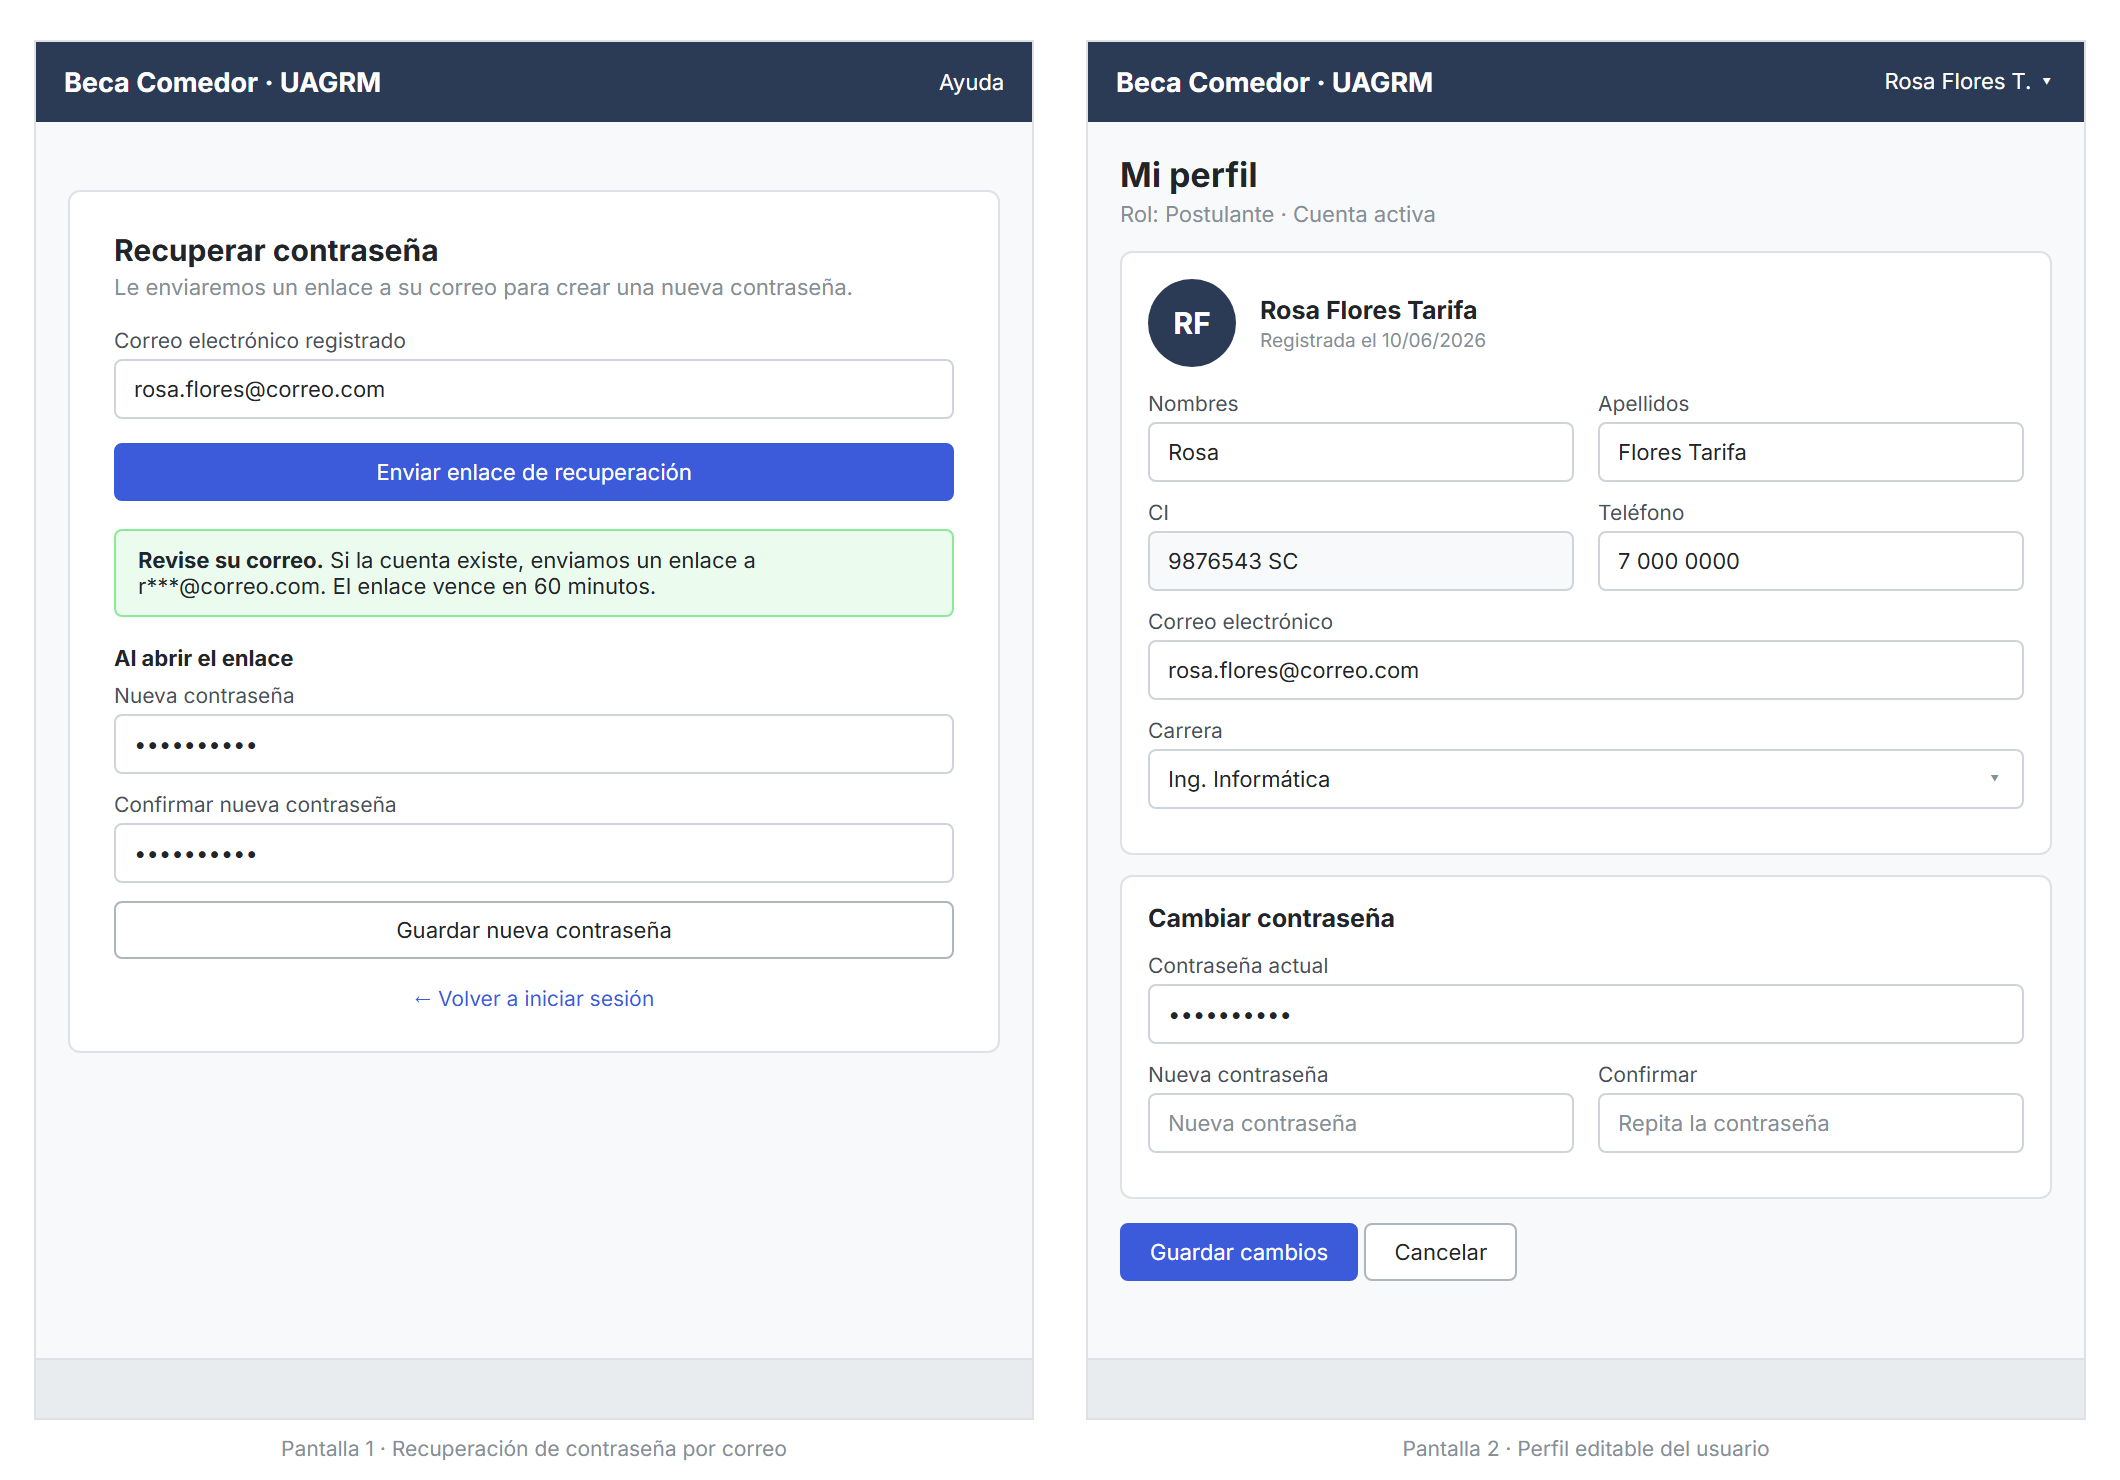
\includegraphics[width=\textwidth,height=0.75\textheight,keepaspectratio]{images/140_Mockup_CU15_Recuperar_contrasena_perfil.png}

\smallskip
\noindent\raggedright\textit{Nota.} Elaboración propia.
\end{figure}



\Needspace{0.9\textheight}
\wfb{\wn{7}.5.16. Interfaz CU-16 Digitalizar y adjuntar documentos}\label{sec:cap7_interfaz_cu16}

La Figura~\ref{fig:mockup_cu16} presenta la maqueta de interfaz del CU-16.

\begin{figure}[H]
\caption{Maqueta de interfaz del CU-16 Digitalizar y adjuntar documentos}
\label{fig:mockup_cu16}
\centering
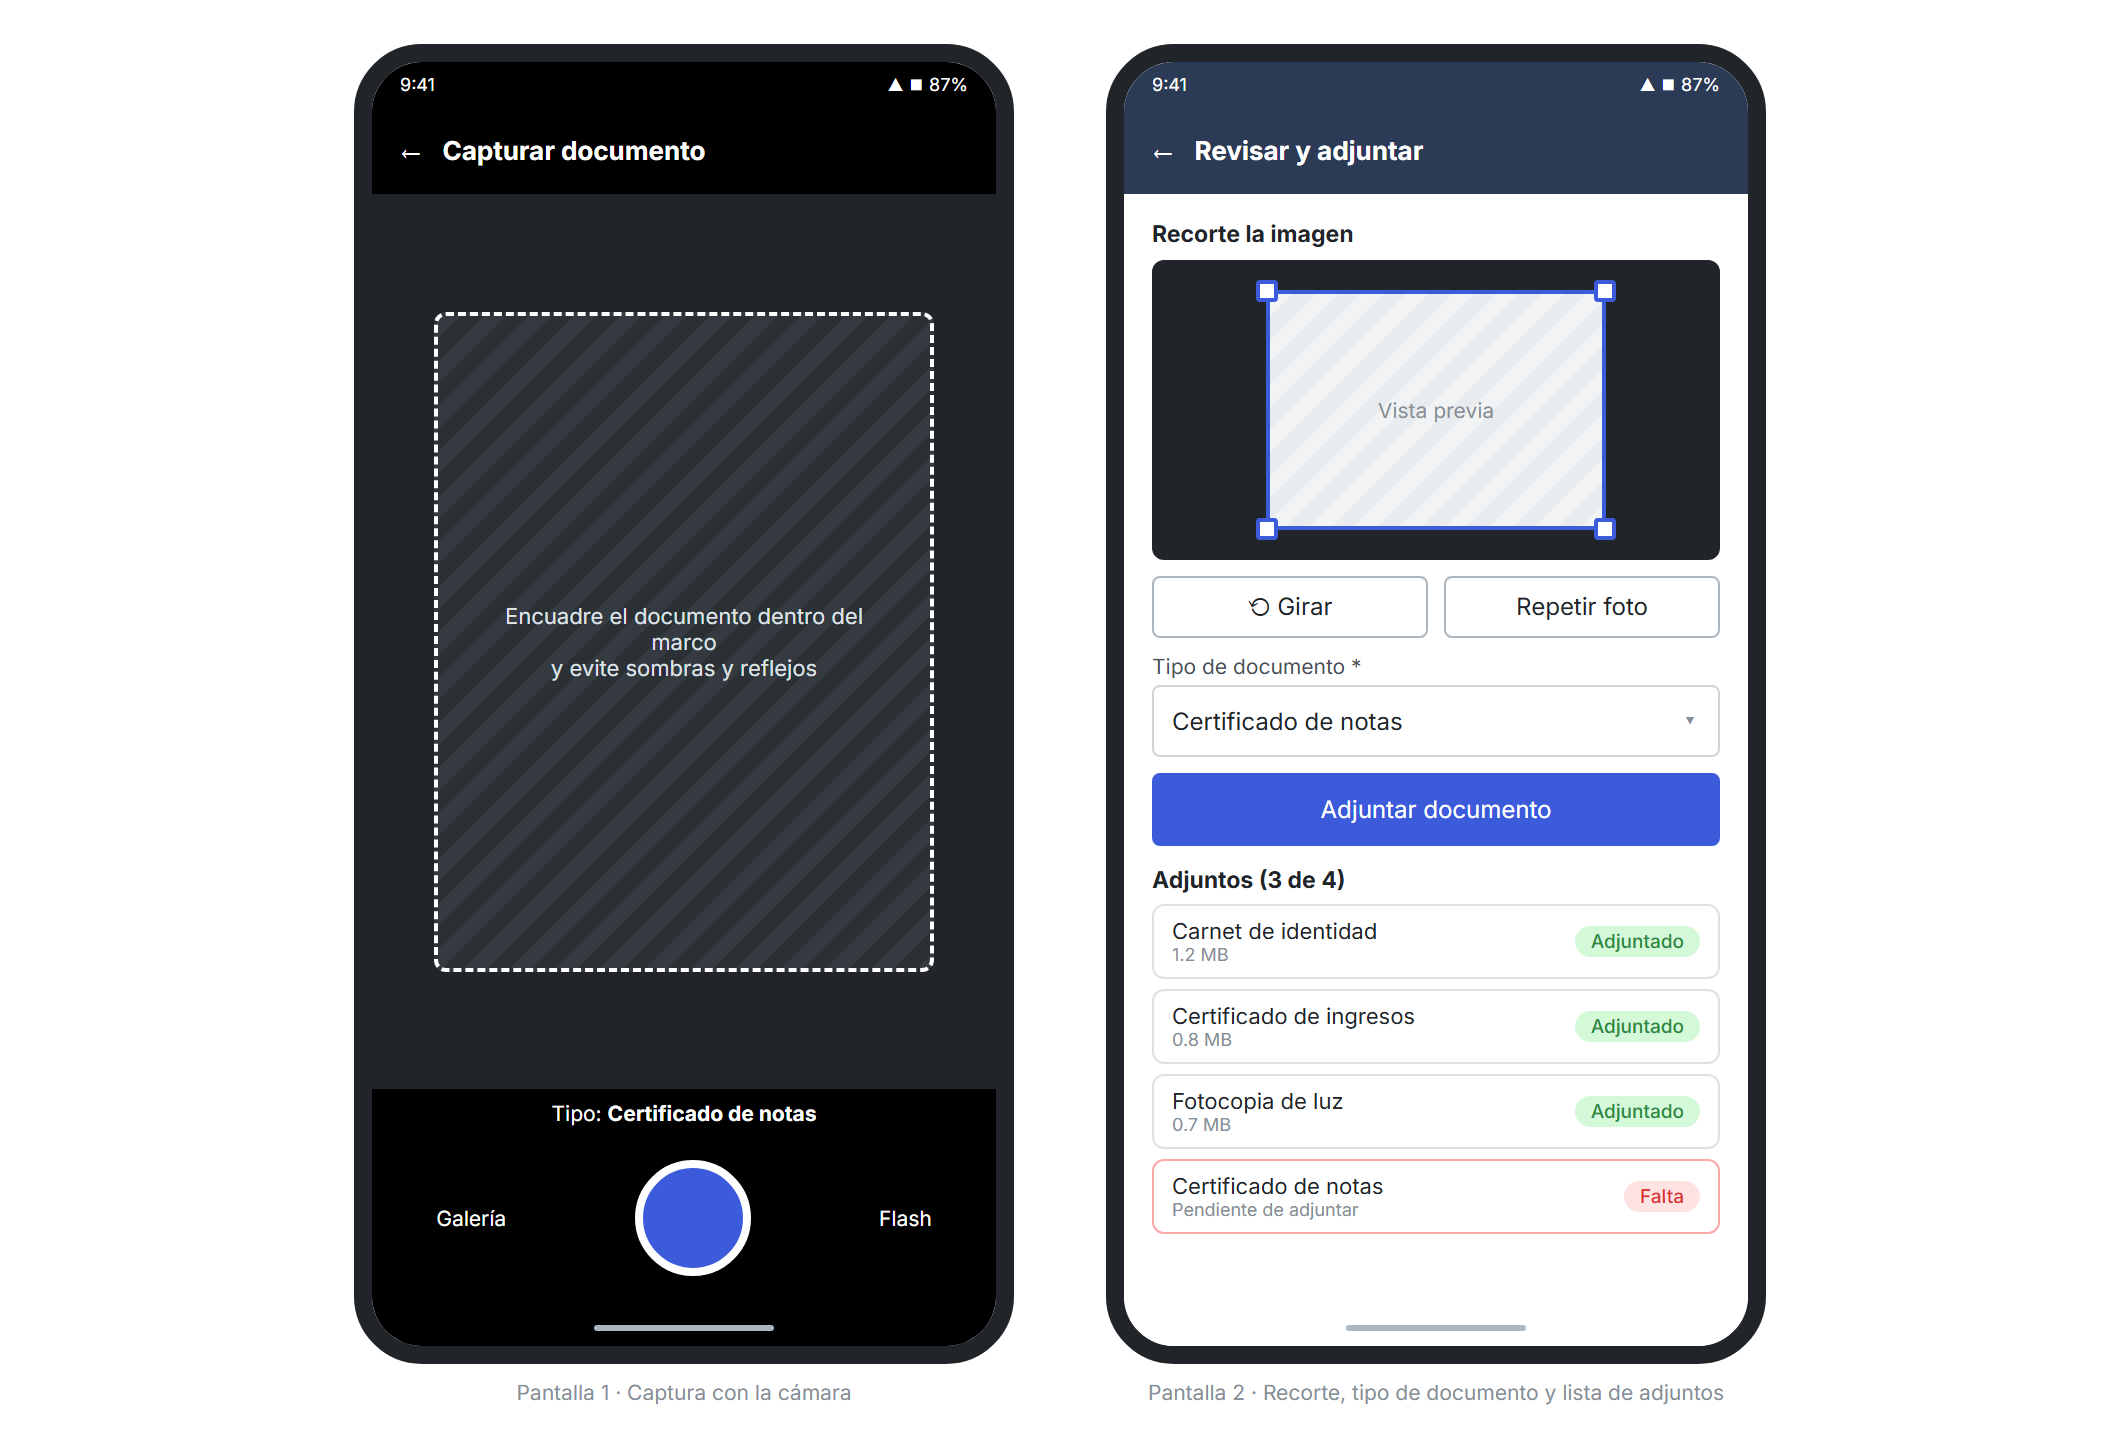
\includegraphics[width=\textwidth,height=0.75\textheight,keepaspectratio]{images/141_Mockup_CU16_Digitalizar_documentos.png}

\smallskip
\noindent\raggedright\textit{Nota.} Elaboración propia.
\end{figure}



\Needspace{0.9\textheight}
\wfb{\wn{7}.5.17. Interfaz CU-17 Guardar borrador de postulación}\label{sec:cap7_interfaz_cu17}

La Figura~\ref{fig:mockup_cu17} presenta la maqueta de interfaz del CU-17.

\begin{figure}[H]
\caption{Maqueta de interfaz del CU-17 Guardar borrador de postulación}
\label{fig:mockup_cu17}
\centering
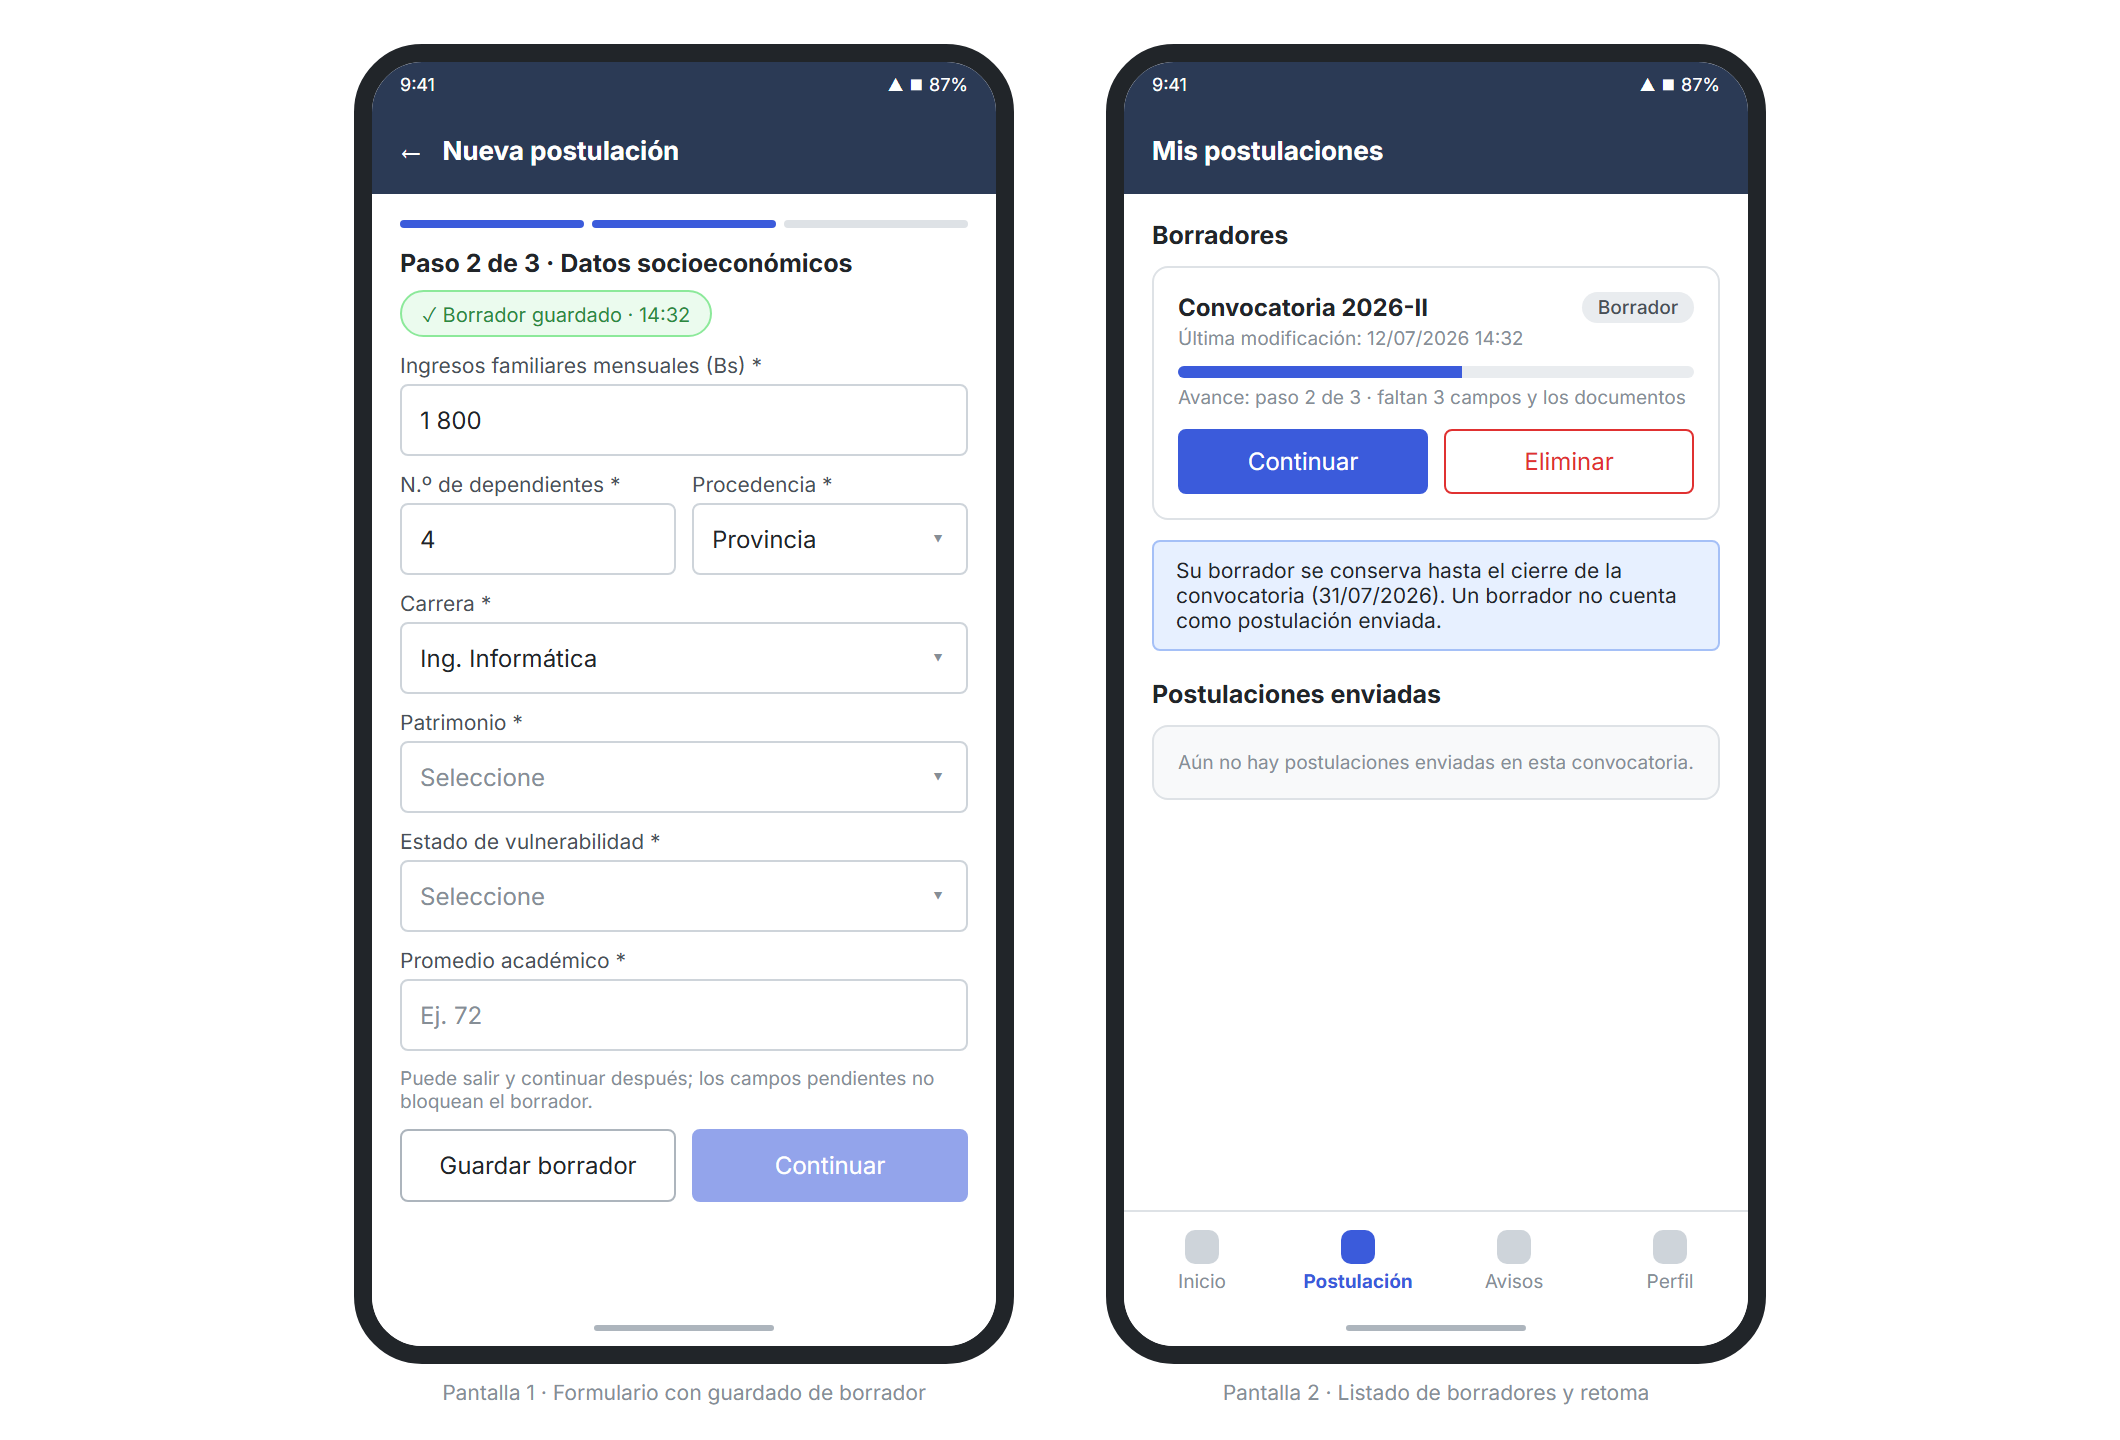
\includegraphics[width=\textwidth,height=0.75\textheight,keepaspectratio]{images/142_Mockup_CU17_Guardar_borrador.png}

\smallskip
\noindent\raggedright\textit{Nota.} Elaboración propia.
\end{figure}



\Needspace{0.9\textheight}
\wfb{\wn{7}.5.18. Interfaz CU-18 Validar elegibilidad y duplicados}\label{sec:cap7_interfaz_cu18}

La Figura~\ref{fig:mockup_cu18} presenta la maqueta de interfaz del CU-18.

\begin{figure}[H]
\caption{Maqueta de interfaz del CU-18 Validar elegibilidad y duplicados}
\label{fig:mockup_cu18}
\centering
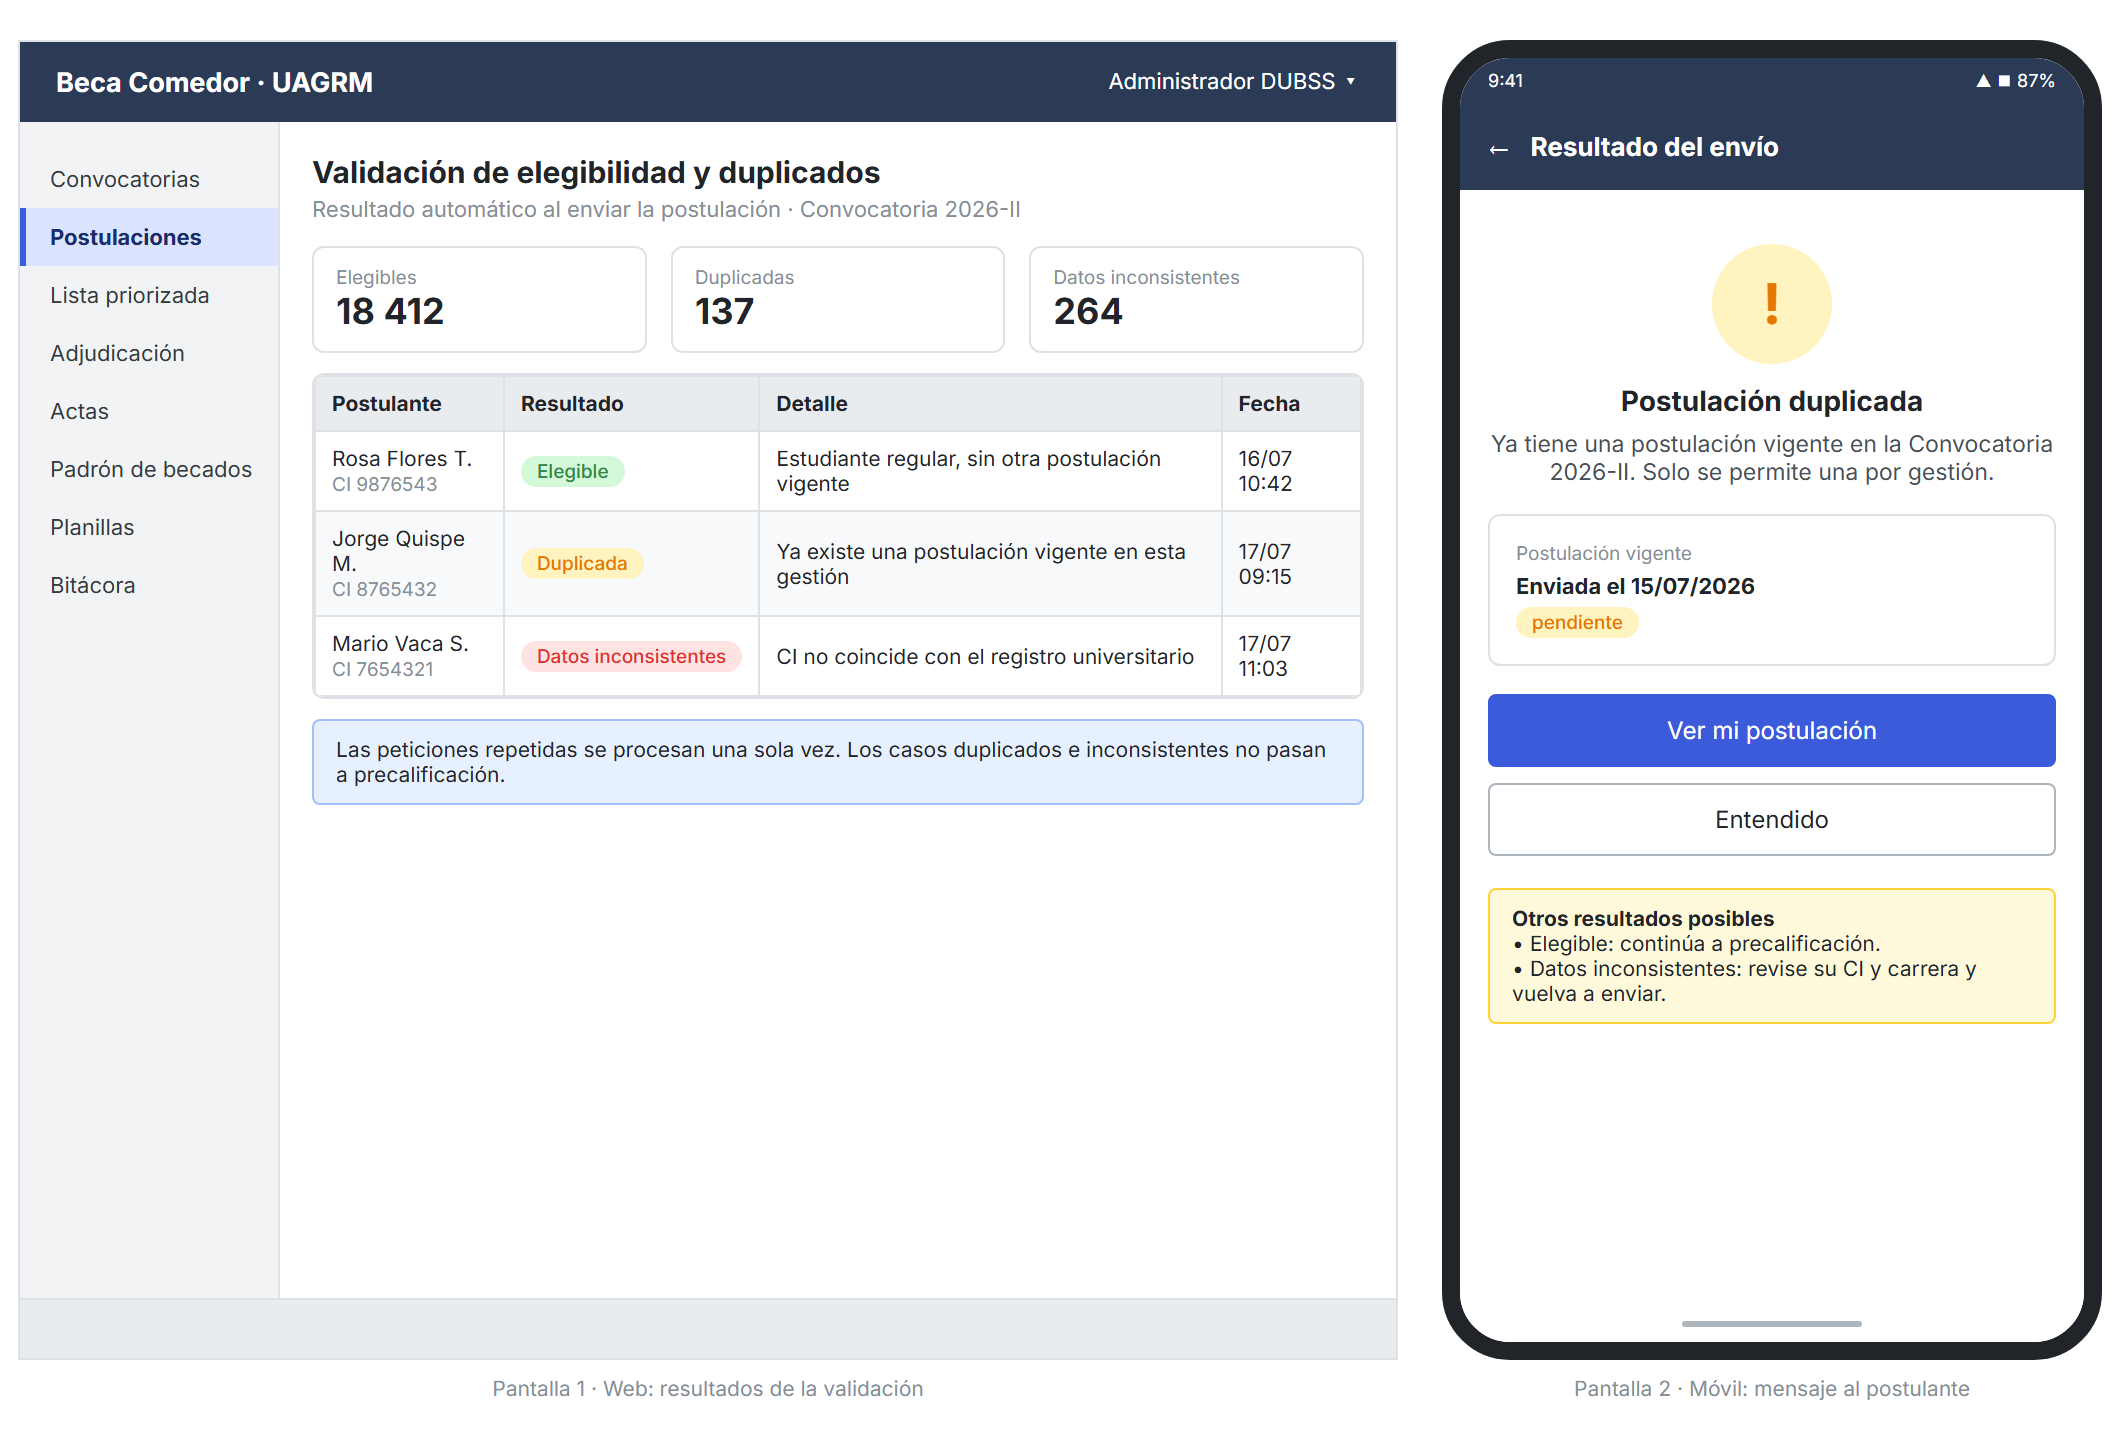
\includegraphics[width=\textwidth,height=0.75\textheight,keepaspectratio]{images/143_Mockup_CU18_Validar_elegibilidad.png}

\smallskip
\noindent\raggedright\textit{Nota.} Elaboración propia.
\end{figure}



\Needspace{0.9\textheight}
\wfb{\wn{7}.5.19. Interfaz CU-19 Devolver postulación para corrección}\label{sec:cap7_interfaz_cu19}

La Figura~\ref{fig:mockup_cu19} presenta la maqueta de interfaz del CU-19.

\begin{figure}[H]
\caption{Maqueta de interfaz del CU-19 Devolver postulación para corrección}
\label{fig:mockup_cu19}
\centering
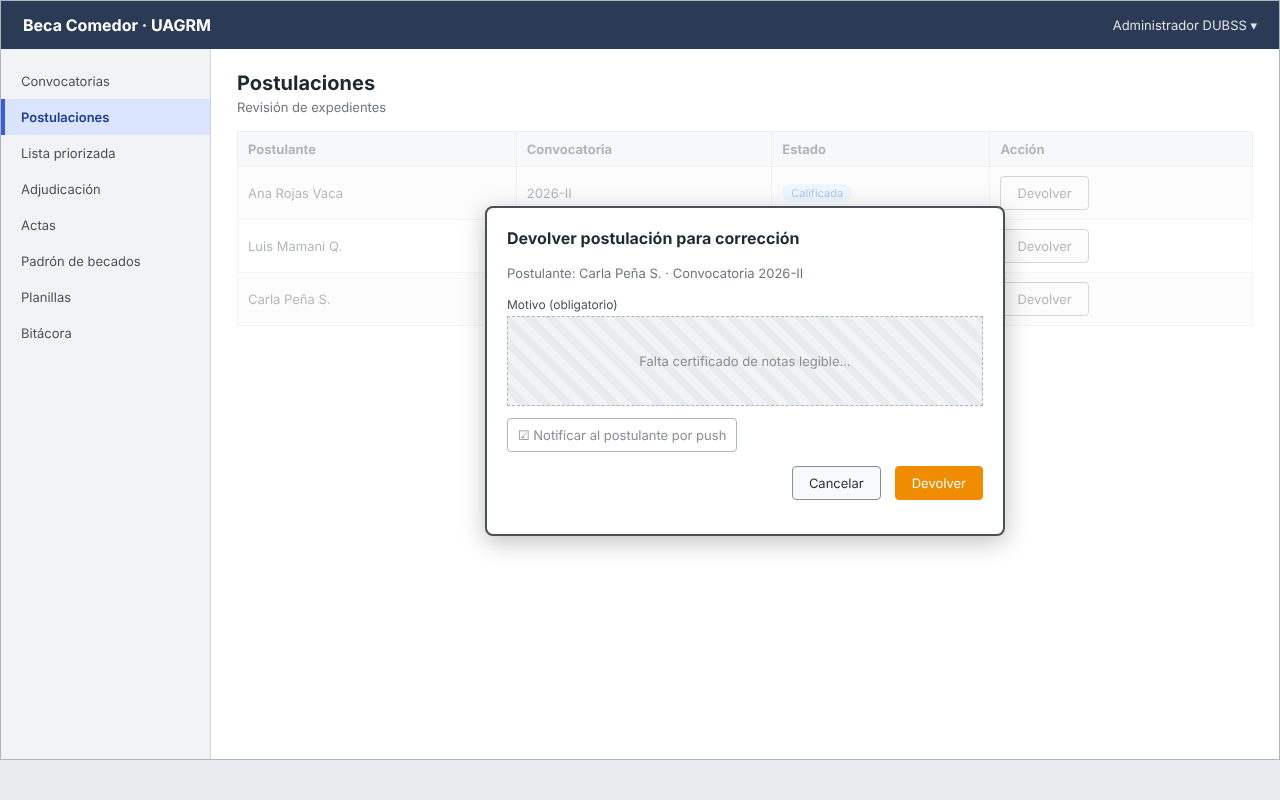
\includegraphics[width=\textwidth,height=0.75\textheight,keepaspectratio]{images/113_Mockup_CU19_Devolver_para_correccion.png}

\smallskip
\noindent\raggedright\textit{Nota.} Elaboración propia.
\end{figure}


\Needspace{0.9\textheight}
\wfb{\wn{7}.5.20. Interfaz CU-20 Archivar o rechazar postulación}\label{sec:cap7_interfaz_cu20}

La Figura~\ref{fig:mockup_cu20} presenta la maqueta de interfaz del CU-20.

\begin{figure}[H]
\caption{Maqueta de interfaz del CU-20 Archivar o rechazar postulación}
\label{fig:mockup_cu20}
\centering
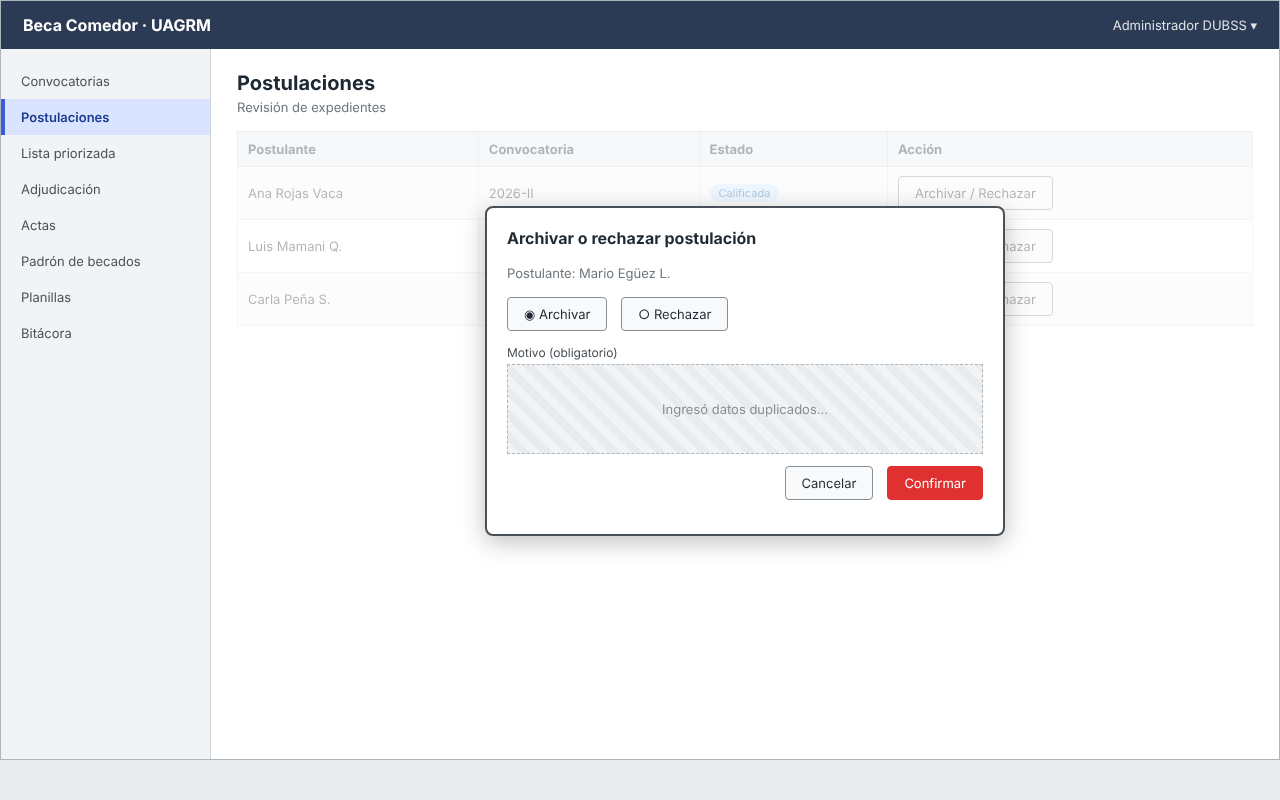
\includegraphics[width=\textwidth,height=0.75\textheight,keepaspectratio]{images/114_Mockup_CU20_Archivar_o_rechazar_postulacion.png}

\smallskip
\noindent\raggedright\textit{Nota.} Elaboración propia.
\end{figure}


\Needspace{0.9\textheight}
\wfb{\wn{7}.5.21. Interfaz CU-21 Notificar finalistas, registrar entrega de documentación física y publicar comunicados/avisos}\label{sec:cap7_interfaz_cu21}

La Figura~\ref{fig:mockup_cu21} presenta la maqueta de interfaz del CU-21.

\begin{figure}[H]
\caption{Maqueta de interfaz del CU-21 Notificar finalistas, registrar entrega de documentación física y publicar comunicados/avisos}
\label{fig:mockup_cu21}
\centering
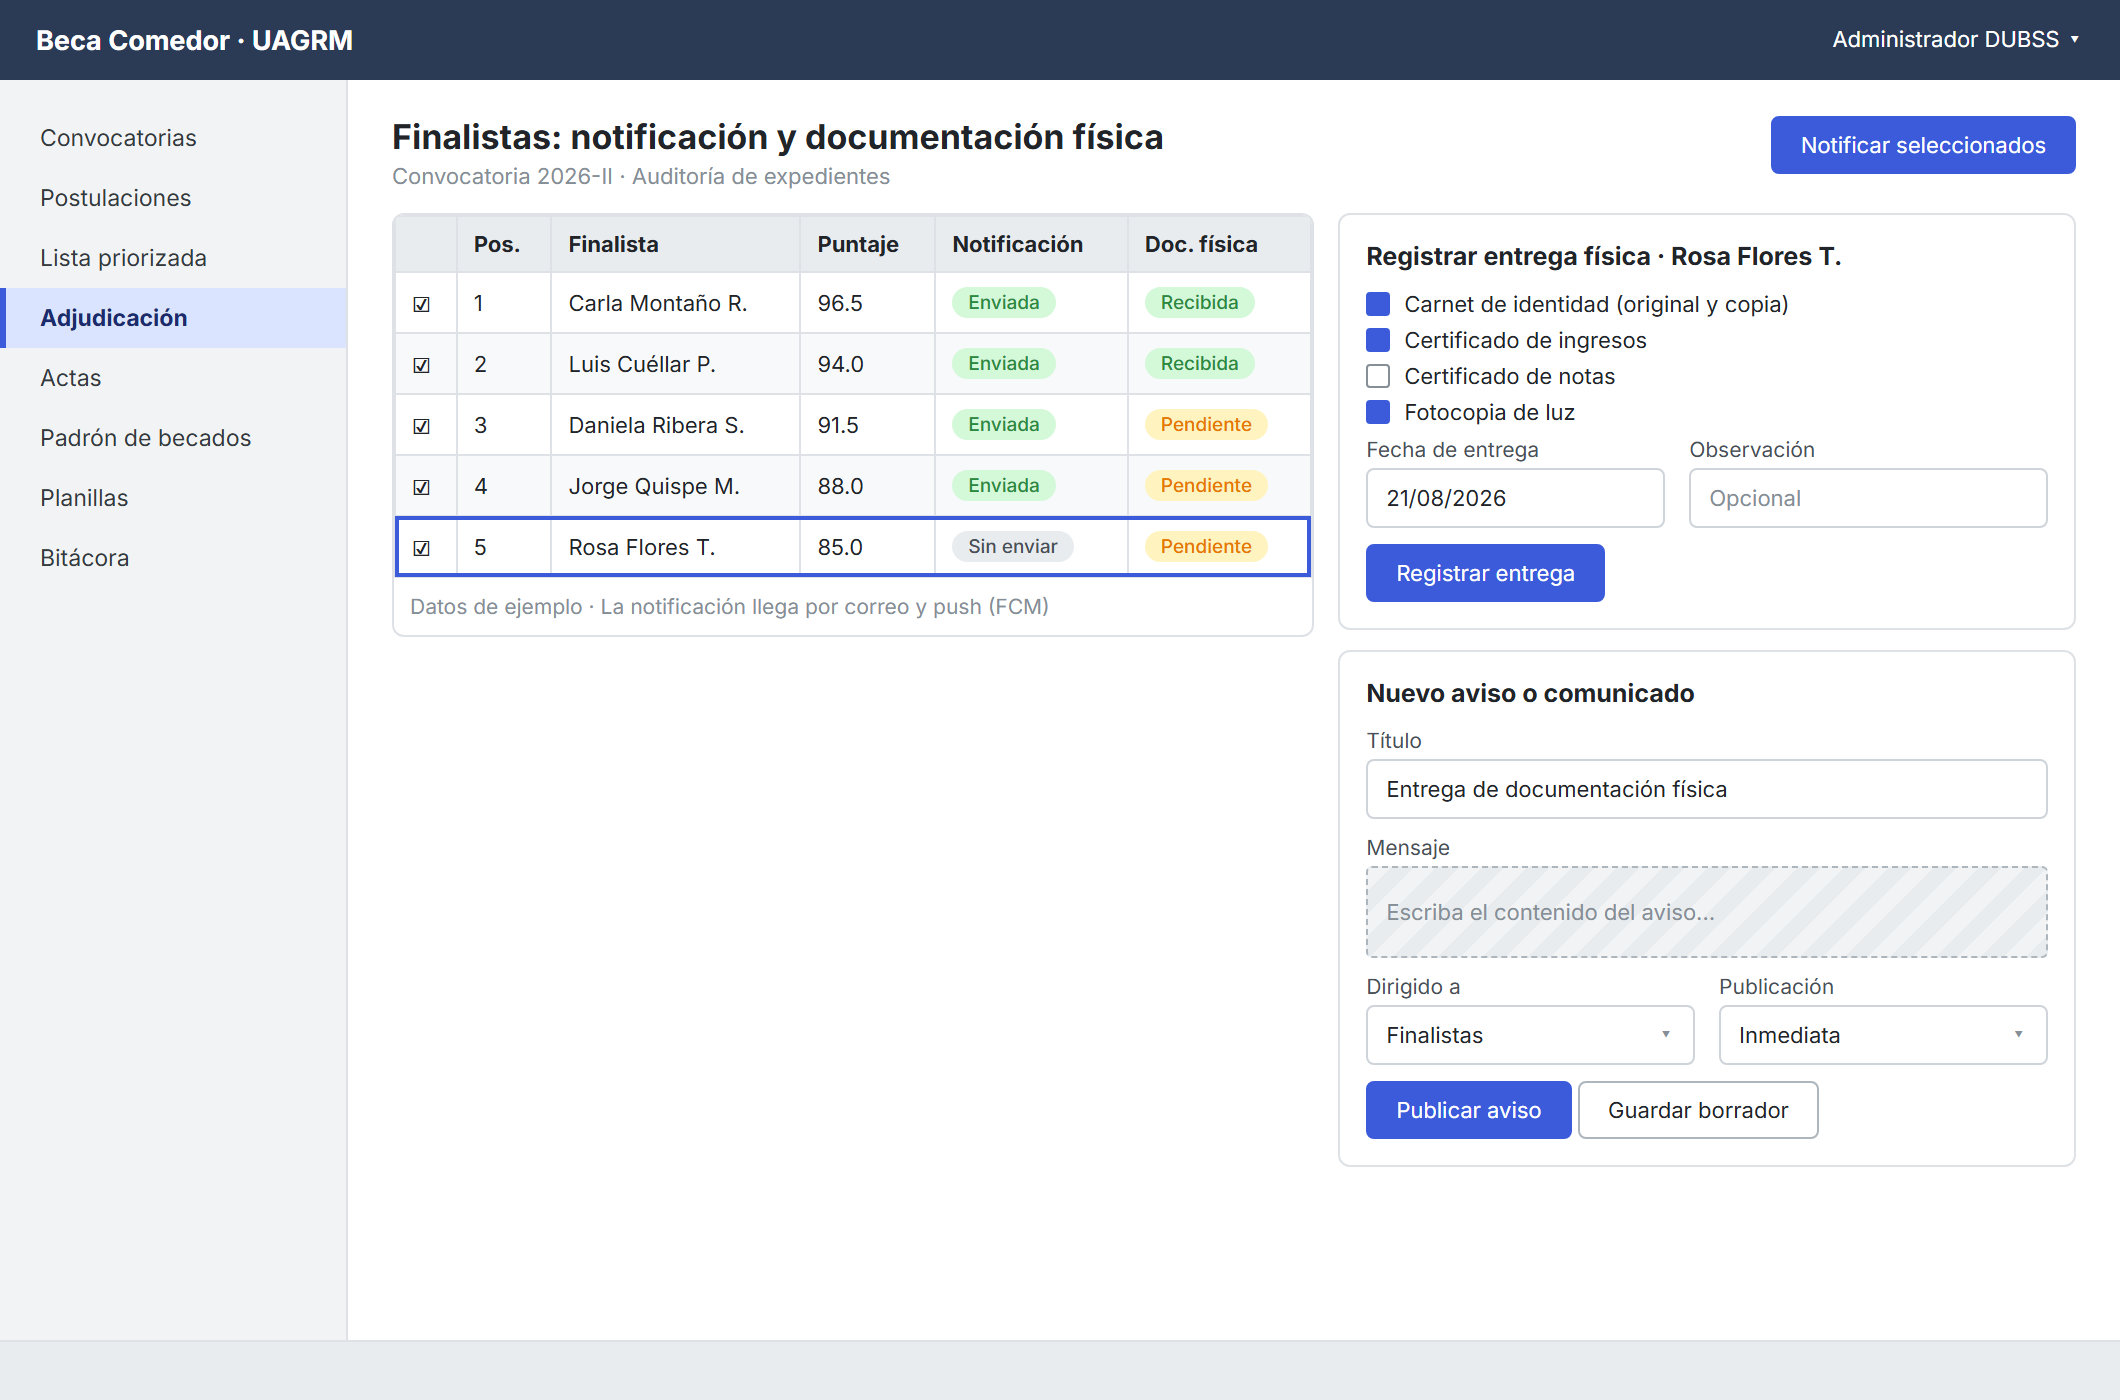
\includegraphics[width=\textwidth,height=0.75\textheight,keepaspectratio]{images/144_Mockup_CU21_Notificar_finalistas_avisos.png}

\smallskip
\noindent\raggedright\textit{Nota.} Elaboración propia.
\end{figure}



\Needspace{0.9\textheight}
\wfb{\wn{7}.5.22. Interfaz CU-22 Publicar resultados de adjudicación}\label{sec:cap7_interfaz_cu22}

La Figura~\ref{fig:mockup_cu22} presenta la maqueta de interfaz del CU-22.

\begin{figure}[H]
\caption{Maqueta de interfaz del CU-22 Publicar resultados de adjudicación}
\label{fig:mockup_cu22}
\centering
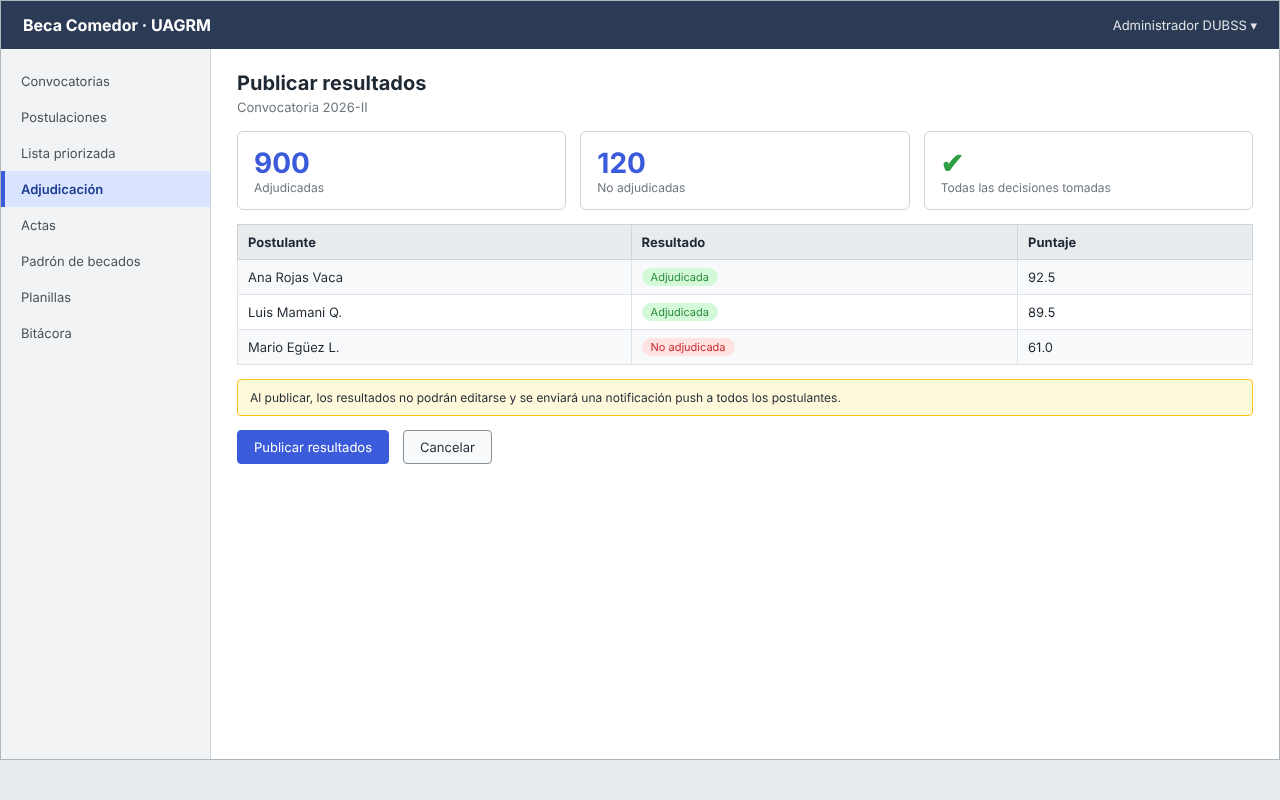
\includegraphics[width=\textwidth,height=0.75\textheight,keepaspectratio]{images/115_Mockup_CU22_Publicar_resultados.png}

\smallskip
\noindent\raggedright\textit{Nota.} Elaboración propia.
\end{figure}


\Needspace{0.9\textheight}
\wfb{\wn{7}.5.23. Interfaz CU-23 Gestionar padrón de becados (baja, suspensión, reemplazo)}\label{sec:cap7_interfaz_cu23}

La Figura~\ref{fig:mockup_cu23} presenta la maqueta de interfaz del CU-23.

\begin{figure}[H]
\caption{Maqueta de interfaz del CU-23 Gestionar padrón de becados (baja, suspensión, reemplazo)}
\label{fig:mockup_cu23}
\centering
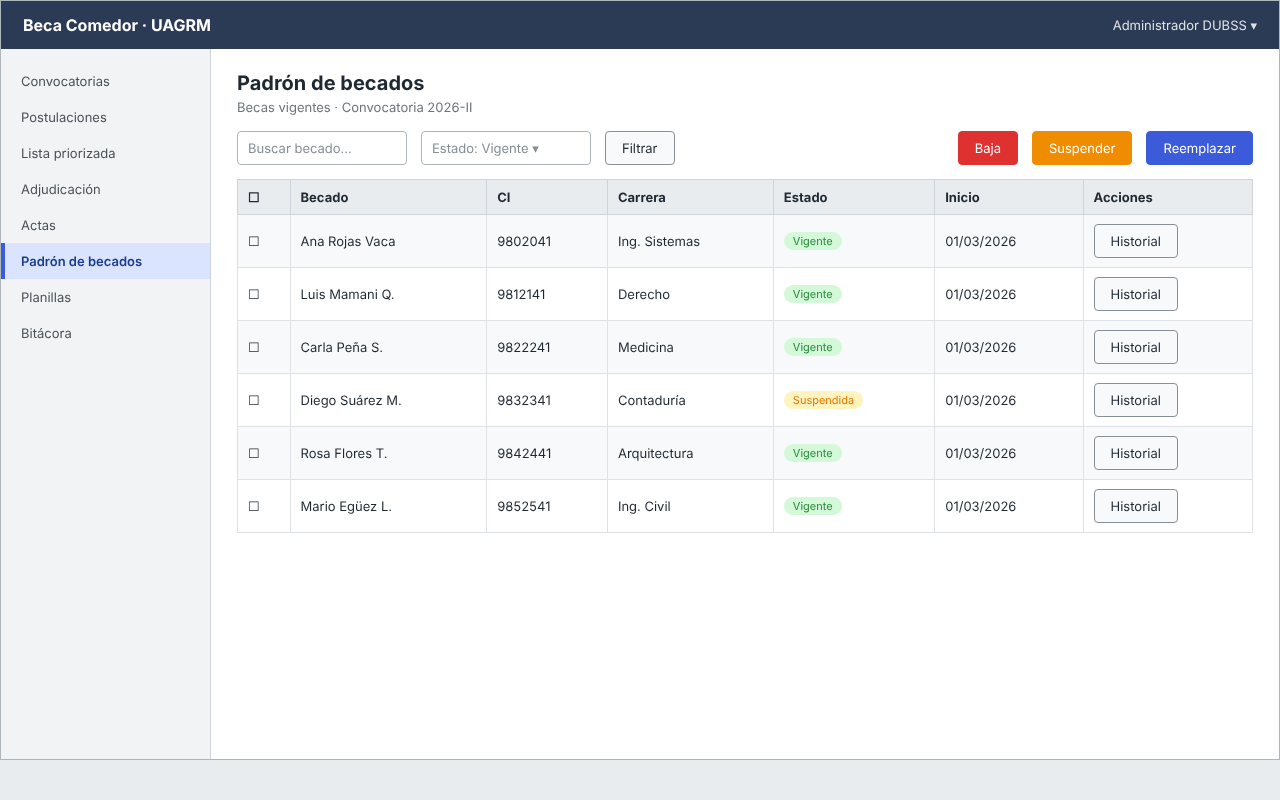
\includegraphics[width=\textwidth,height=0.75\textheight,keepaspectratio]{images/116_Mockup_CU23_Padron_de_becados.png}

\smallskip
\noindent\raggedright\textit{Nota.} Elaboración propia.
\end{figure}


\Needspace{0.9\textheight}
\wfb{\wn{7}.5.24. Interfaz CU-24 Consultar historial de asistencia y estado de beca}\label{sec:cap7_interfaz_cu24}

La Figura~\ref{fig:mockup_cu24} presenta la maqueta de interfaz del CU-24.

\begin{figure}[H]
\caption{Maqueta de interfaz del CU-24 Consultar historial de asistencia y estado de beca}
\label{fig:mockup_cu24}
\centering
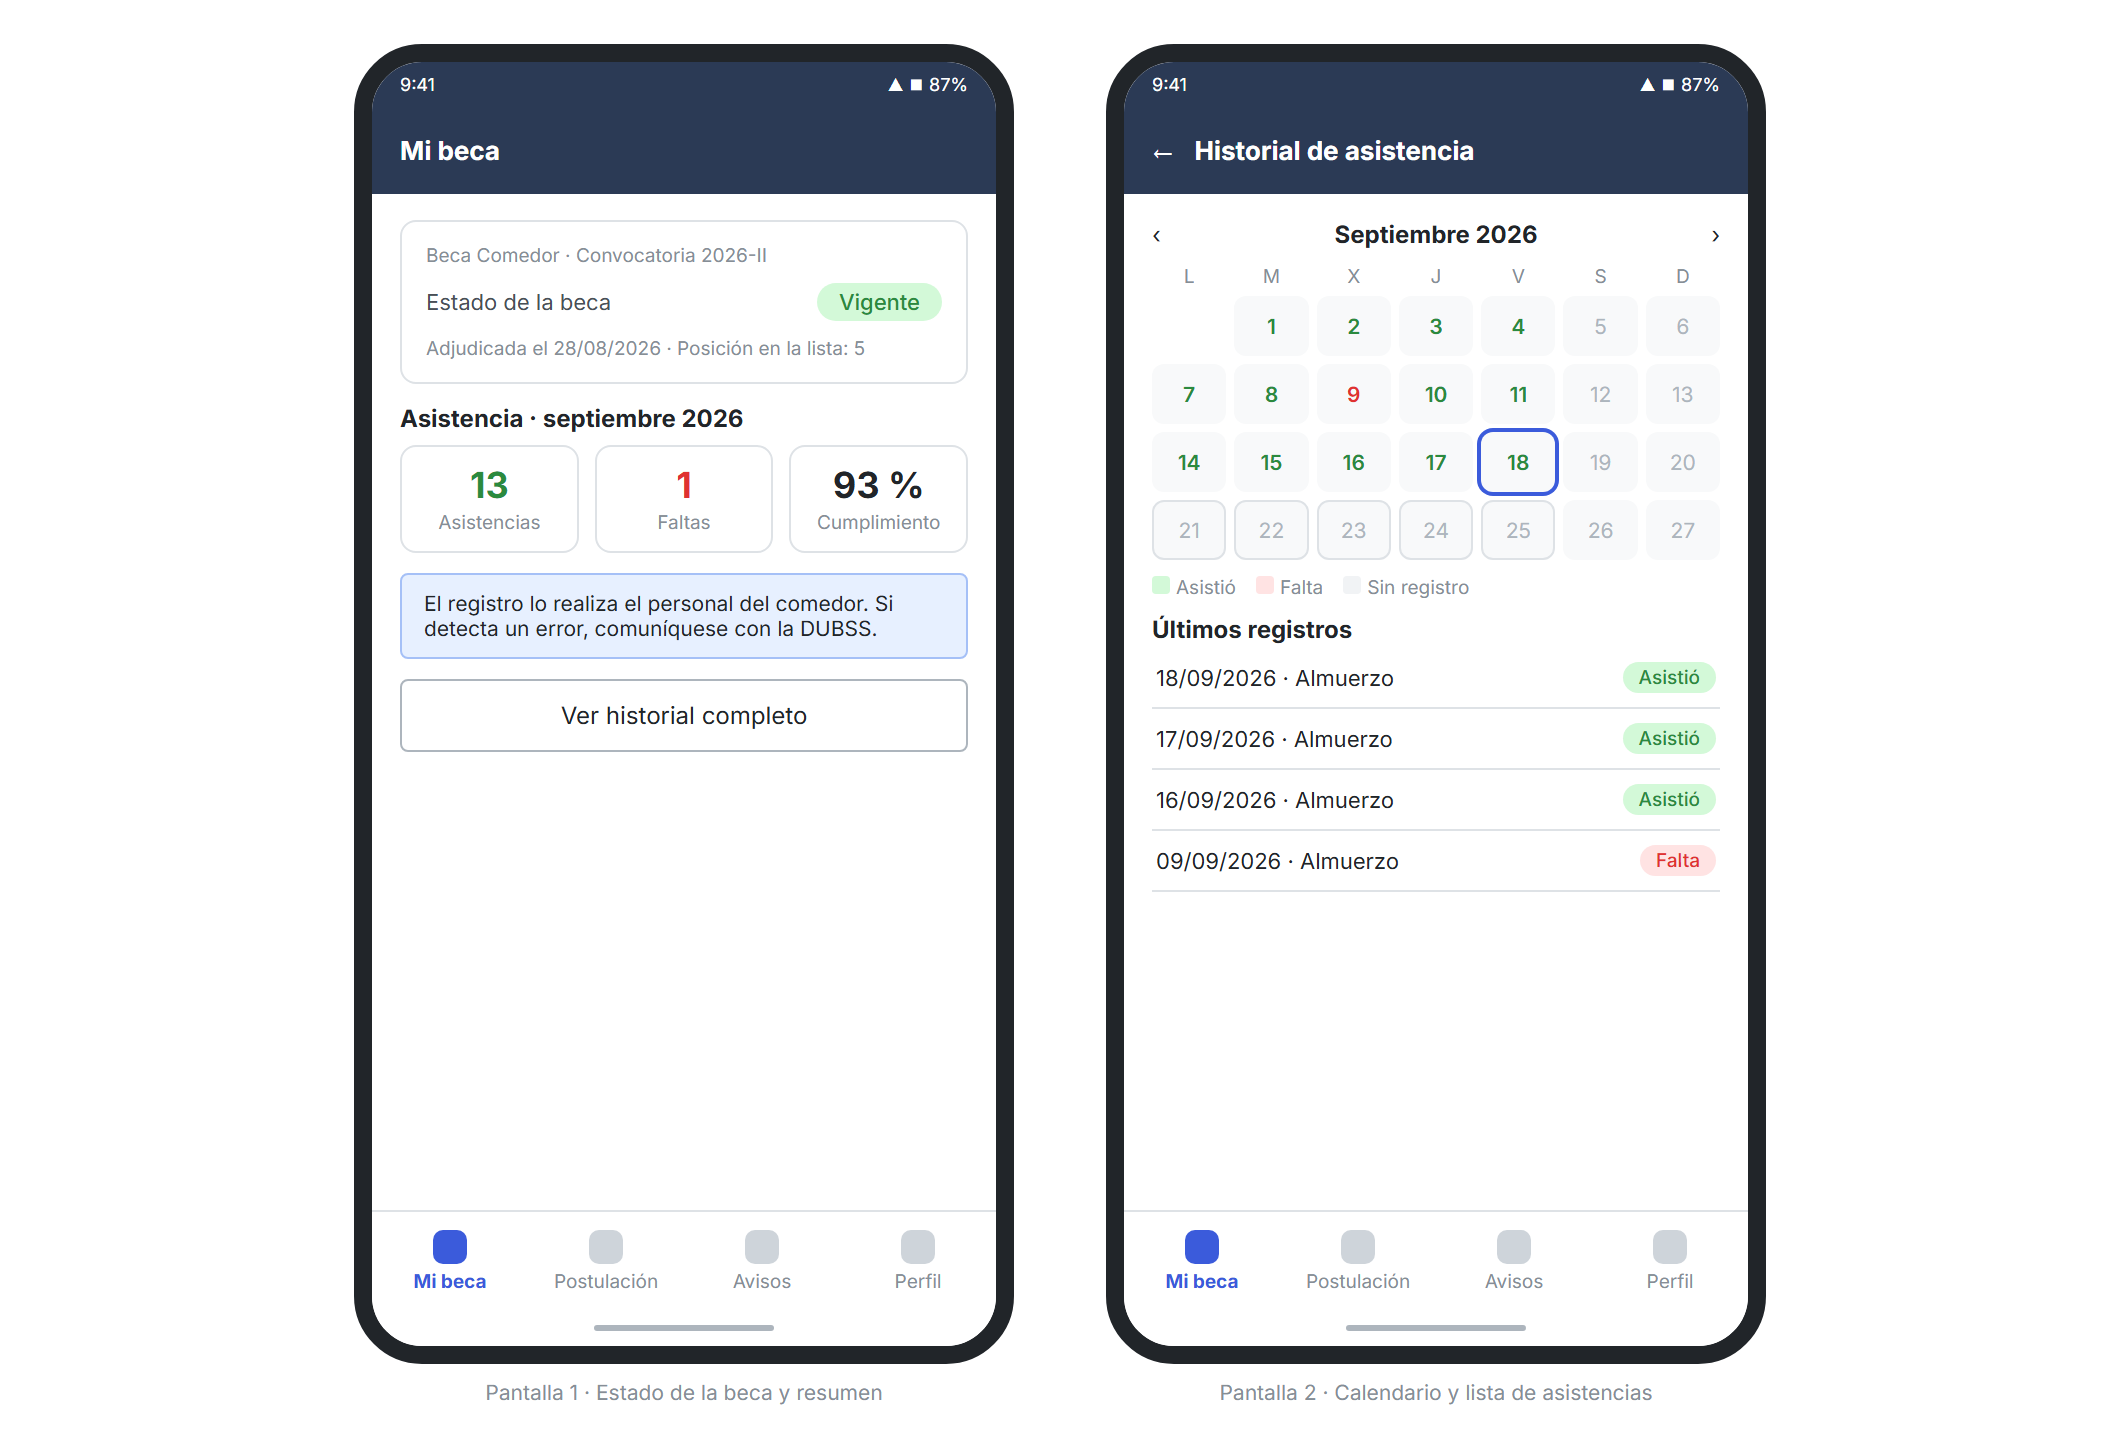
\includegraphics[width=\textwidth,height=0.75\textheight,keepaspectratio]{images/145_Mockup_CU24_Historial_asistencia.png}

\smallskip
\noindent\raggedright\textit{Nota.} Elaboración propia.
\end{figure}



\Needspace{0.9\textheight}
\wfb{\wn{7}.5.25. Interfaz CU-25 Consultar bitácora de acciones}\label{sec:cap7_interfaz_cu25}

La Figura~\ref{fig:mockup_cu25} presenta la maqueta de interfaz del CU-25.

\begin{figure}[H]
\caption{Maqueta de interfaz del CU-25 Consultar bitácora de acciones}
\label{fig:mockup_cu25}
\centering
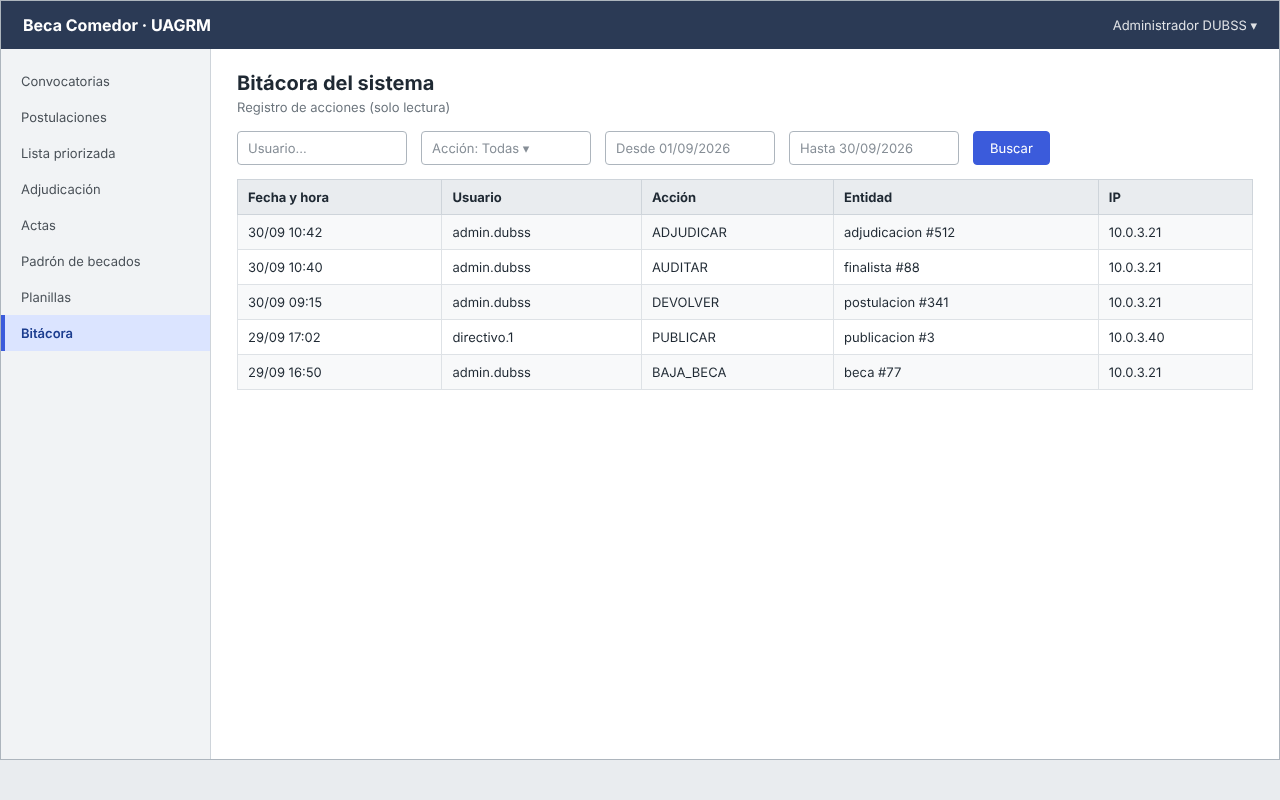
\includegraphics[width=\textwidth,height=0.75\textheight,keepaspectratio]{images/117_Mockup_CU25_Bitacora.png}

\smallskip
\noindent\raggedright\textit{Nota.} Elaboración propia.
\end{figure}


\Needspace{0.9\textheight}
\wfb{\wn{7}.5.26. Interfaz CU-26 Parametrizar modelo de preselección y reprocesar puntajes}\label{sec:cap7_interfaz_cu26}

La Figura~\ref{fig:mockup_cu26} presenta la maqueta de interfaz del CU-26.

\begin{figure}[H]
\caption{Maqueta de interfaz del CU-26 Parametrizar modelo de preselección y reprocesar puntajes}
\label{fig:mockup_cu26}
\centering
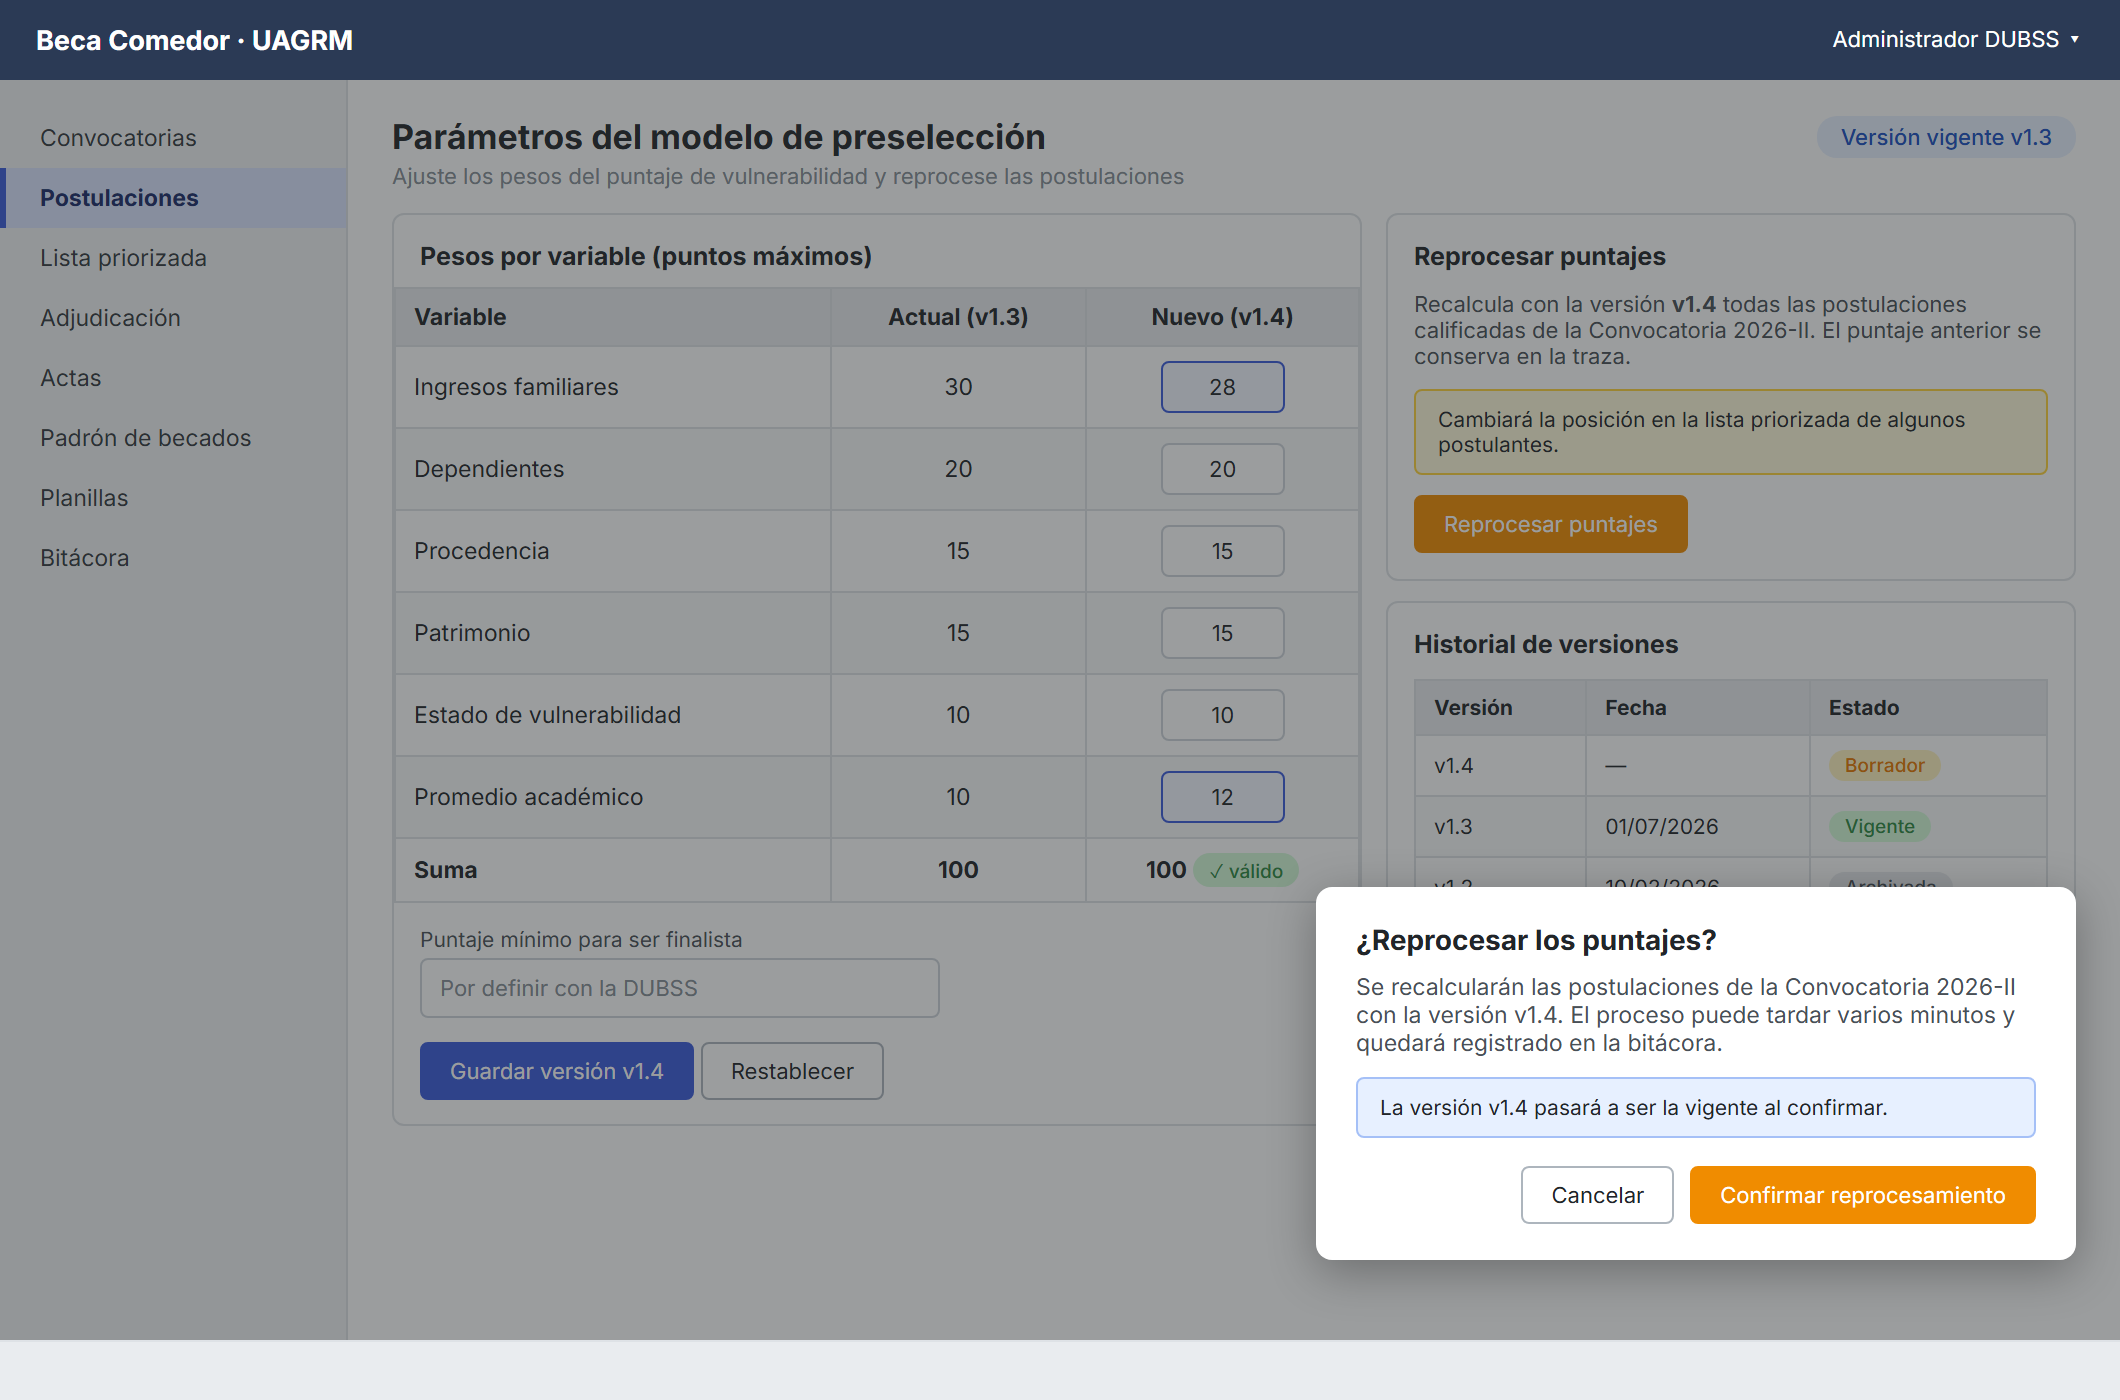
\includegraphics[width=\textwidth,height=0.75\textheight,keepaspectratio]{images/146_Mockup_CU26_Parametrizar_modelo.png}

\smallskip
\noindent\raggedright\textit{Nota.} Elaboración propia.
\end{figure}



